\documentclass[a4paper,11pt]{article}

\makeatletter
\newcommand\appendix@section[1]{%
  \refstepcounter{section}%
  \orig@section*{Appendix \@Alph\c@section: #1}%
  \addcontentsline{toc}{section}{Appendix \@Alph\c@section: #1}%
}
\let\orig@section\section
\g@addto@macro\appendix{\let\section\appendix@section}
\makeatother


\usepackage{graphicx}
\usepackage{pifont}
\usepackage{ulem}
\usepackage{supertabular}
\usepackage{rotating}
\usepackage{latexsym}
\usepackage{placeins}
\usepackage{verbatim}
\usepackage{appendix}
\voffset -1.5cm
\hoffset 0.0cm
\textheight 25cm
\textwidth 16cm
\topmargin 0.0cm
\oddsidemargin 0.0cm
\evensidemargin 0.0cm

\newcommand{\VROT}[1]{\begin{turn}{90}#1\end{turn}}     % vertical text
\def\X{$\surd$}     % tick symbol

\usepackage{hyperref}%                   % Utilisation de HyperTeX

\hypersetup{
    pdfauthor   = {Gilles Mouchard},%
    pdftitle    = {UNISIM\\ TMS320C3X Manual},%
    pdfsubject  = {UNISIM\\ TMS320C3X Manual},%
    pdfkeywords = {simulation framework, architectural exploration, embedded system design, system verification},%
    pdfcreator  = {rubber},%
    pdfproducer = {rubber}
}

\title{UNISIM\\ TMS320C3X Manual}
\author{Gilles Mouchard \\Daniel Gracia P\'erez \\Reda Nouacer \\ \\CEA List}
\date{}

\begin{document}
% \addtolength{\hoffset}{-2.0cm}
% \addtolength{\voffset}{-2.0cm}


\maketitle
\section{User guide}

\subsection{Simulator features}

The TMS320C3X is a 32-bit floating-point DSP from Texas Instrument.
The UNISIM TMS320C3X 2.0 simulator features:
\begin{itemize}
\item Written for SystemC TLM 2.0
\item Simulation of the TMS320C3X instruction set
\item A simulation speed average around 11 MIPS and up to 14 MIPS on a 2.4 Ghz Core2 Duo machine under Linux
\item Support for instruction cache
\item Support for TI COFF v0, v1, and v2 (either with big-endian or little-endian headers)
\item Built-in debugger (Inline Debugger)
\item Support for GDB serial remote protocol (GDB server)
\item Support for TI C I/O
\end{itemize}

\begin{figure}[!h]
	\begin{center}
		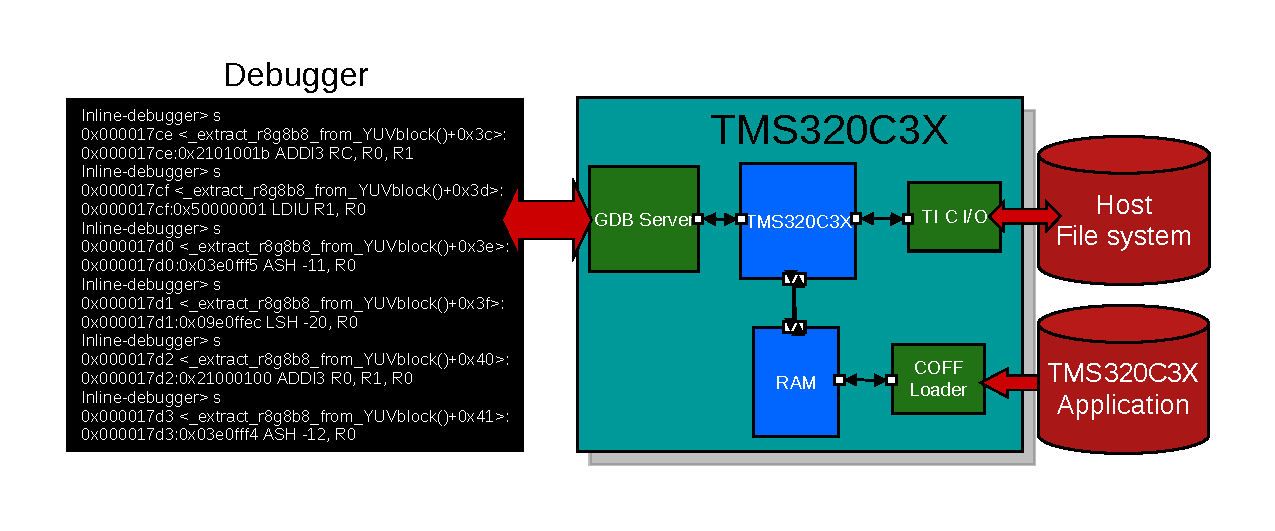
\includegraphics[width=\textwidth]{tms320c3x/fig_tms320c3x.pdf}
	\end{center}
	\caption{TMS320C3X simplified schematic.}
	\label{fig:tms320c3x}
\end{figure}

\subsection{Status of implementation}

The UNISIM TMS320C3X has been developed using the following documentation:
\begin{itemize}
\item TMS320C3x User’s Guide (SPRU031F, 2558539-9761 revision L, March 2004)
\item TMS320C3x/C4x Assembly Language Tools User’s Guide (SPRU035D, June 1998)
\item TMS320C3x/C4x Optimizing C Compiler User’s Guide (SPRU034H, June 1998)
\end{itemize}

The simulator current implementation completely decodes the TMS320C3X instruction set.
All registers are present but no on-chip devices are implemented.
The simulator has complete support for:
\begin{itemize}
\item integer instructions (2-ops, 3-ops, parallel ops, load/store)
\item floating point instructions (2-ops, 3-ops, parallel ops, load/store)
\item control instructions (branches, delayed branches, RPTS, RPTB), but \texttt{iack} and \texttt{swi} instructions
\item interlocked instructions, but \texttt{sigi} instruction
\item power instructions
\item interrupt handling
\end{itemize}

The current status of the simulator allows to run any integer or floating-point benchmark.
However, during the validation process of the UNISIM TMS320C3X simulator, four hardware bugs have been found on our development board, and one software bug in Code Composer.
The UNISIM TMS320C3X simulator can emulate these bugs (see Section~\ref{tms320c3x_configuration}) if they are enabled:
\begin{itemize}
\item \texttt{LDF || LDF} bug: From our experiments on the development board, uncomprehensibly \texttt{src1} is not correctly transformed to a valid \texttt{0.0} when the \texttt{src1} exponent is \texttt{0x80}. Simulator parameter \texttt{cpu.enable-parallel-load-bug} enables this bug.
\item \texttt{STF || STF} and \texttt{STI || STI} bugs: From our experiments on the development board, the first store is never performed. Simulator parameter \texttt{cpu.enable-parallel-store-bug} enables these bugs.
\item \texttt{RND} bug: TMS320C3x User’s Guide says that the \texttt{rnd} instruction does not affect the \texttt{Z} flag however the real hardware systematically sets \texttt{Z} to 0. Simulator parameter \texttt{cpu.enable-rnd-bug} enables this bug.
\item \texttt{lseek} bug: From our experiments on the development board, function \texttt{lseek} from \texttt{RTS30.LIB} has a 32-bit return value truncated to 16 bits. Simulator parameter \texttt{ti-c-io.enable-lseek-bug} enables this bug.
\item floating point instructions bug: All the float instructions can use non-extended registers (all the registers different than \texttt{R0-R7}). However their behavior when using non-extended registers is not documented, and from our experiments on the development board their behavior is unexpected. By default, the simulator does not allow the use of non-extended registers for float instructions (obviously with the exception of the \texttt{FIX} and \texttt{FLOAT} instructions when the use of non-extended registers is documented). Simulator parameter \texttt{cpu.enable-float-ops-with-non-ext-regs} allows the use of non-extended registers for float instructions. Note that the behavior of the instructions when using non-extended registers has been deduced from our experiments with the evaluation board, but that they can not be validated due to the lack of documentation and unexpected behavior.
\end{itemize}

\subsection{Compiling the simulator}

Up-to-date instructions for compiling the simulator are available in the \texttt{INSTALL} file.

\subsection{Invoking the simulator}

The general command line format for invoking the simulator is the following:

\begin{verbatim}
unisim-tms320c3x-2.0 [<options>] <binary to simulate>
\end{verbatim}

\noindent The binary to simulate must be a TI's COFF v0, v1 or v2 file. See~\ref{tms320c3x_cross_compiler} to generate such files.
\newline\\
\noindent The command line options of the simulator are:

\begin{itemize}
\item \texttt{--set $<$param=value$>$ or -s $<$param=value$>$}: set value of parameter 'param' to 'value'
\item \texttt{--config $<$XML file$>$ or -c $<$XML file$>$}: configures the simulator with the given XML configuration file
\item \texttt{--get-config $<$XML file$>$ or -g $<$XML file$>$}: get the simulator configuration XML file (you can use it to create your own configuration. This option can be combined with -c to get a new configuration file with existing variables from another file
\item \texttt{--list or -l}: lists all available parameters, their type, and their current value
\item \texttt{--warn or -w}: enable printing of kernel warnings
\item \texttt{--doc $<$Latex file$>$ or -d $<$Latex file$>$}: enable printing a latex documentation
\item \texttt{--version or -v}: displays the program version information
\item \texttt{--share-path $<$path$>$ or -p $<$path$>$}: the path that should be used for the share directory (absolute path)
\item \texttt{--help or -h}: displays this help
\end{itemize}

\subsection{The Texas Instrument cross-compiler for TMS320C3X}
\label{tms320c3x_cross_compiler}

To compile programs for the TMS320C3X simulator, you can use the free evaluation cross-compiler for TMS320C3X running on a Windows host (SPRC147, TMS320C3x DSK Software) available at \url{http://focus.ti.com/docs/toolsw/folders/print/tmdsdsk33.html}.
This cross-compiler also runs under other x86 operating systems such as Linux or MacOSX using Wine, a Windows emulator (\url{http://www.winehq.org/}).

\textit{Note: Be aware that any call to the C standard library requires linking the program with \texttt{RTS30.LIB}.
Moreover, any call to I/O functions (open, close, read, write, printf, \ldots) requires TI C I/O support enabled in the TMS320C3X simulator.}

The cross-compiler tool chain (\texttt{CL30.EXE, LNK30.EXE, ASM30.EXE, MK30.EXE, ar30.EXE, \ldots}) should be in your \texttt{PATH}.
The shell variable \texttt{C\_DIR} points to the location where the cross-compiler should search for the standard C headers and libraries.
Suppose the tool chain is installed in \texttt{C:{\textbackslash}TI}.
Windows users should add the following in their \texttt{AUTOEXEC.BAT}:
\begin{verbatim}
set PATH=C:\TI\TIC3X4X\BIN;%PATH%
set C_DIR=C:\TI\TIC3X4X\INCLUDE;C:\TI\TIC3X4X\LIB
\end{verbatim}
Wine and GNU bash users should add the following in their \texttt{.bashrc}:
\begin{verbatim}
export PATH=${HOME}/.wine/drive_c/TI/TIC3X4X/BIN:${PATH}
export C_DIR=C:\\TI\\TIC3X4X\\INCLUDE\;C:\\TI\\TIC3X4X\\LIB
\end{verbatim}

\subsection{The GNU binutils}

The GNU binutils are a set of open source tools to manipulate binaries. They provide an assembler, a linker, and an object dump utility among others.
The last version, at the time of writing this document, is available at: \url{ftp://ftp.gnu.org/gnu/binutils/binutils-2.19.1.tar.gz}
The GNU binutils support TI COFF v0, v1 and v2 binary files for both TMS320C3X and TMS320C4X targets.

To compile the binutils and install them into \texttt{/opt/c4x-coff}:

\begin{verbatim}
$ ./configure --target=c4x-unknown-coff --prefix=/opt/c4x-coff
$ make
$ make install
\end{verbatim}

A key feature of the GNU binutils is the ability of \texttt{objdump} to dump/disassemble a TI COFF binary for the TMS320C3X.
For instance, the following command will dump file \texttt{test.out} into file \texttt{dump.txt}:

\begin{verbatim}
$ /opt/c4x-coff/bin/c4x-unknown-coff-objdump -D test.out > dump.txt
\end{verbatim}

\subsection{The GNU GDB debugger}

Version 4.16 of GDB was patched to support C3x/C4x (see \url{http://www.elec.canterbury.ac.nz/c4x/doc/c4x-tools.html} and \url{ftp://ftp.rtems.com/pub/c4x-tools}).
We've slightly patched again this port to make it work on a modern Linux distribution.
It runs on 32-bit x86 Linux hosts.
It is available at: \url{http://unisim-vp.org/site/downloads/other/crosstool/c4x-coff-gdb-4.16.tar.gz}.

To build this special version of GDB, do the following commands:
\begin{verbatim}
$ tar x c4x-coff-gdb-4.16.tar.gz
$ cd c4x-coff-gdb-4.16
$ ./build.sh all
\end{verbatim}

That special GDB can connects to the UNISIM TMS320C3X simulator:

\begin{verbatim}
$ unisim-tms320c3x-2.0 -s enable-gdb-server=true -s gdb-server.tcp-port=1234
\end{verbatim}

\begin{verbatim}
$ ./c4-coff-gdb/bin/c4-coff-gdb 
(gdb) set machine 30
(gdb) target remote localhost:1234
\end{verbatim}

\subsection{Simulator configuration}
\label{tms320c3x_configuration}

\noindent The simulator stores its configuration (a set of parameters) in a XML configuration file. 
\newline\\
\noindent The simulator can provide the user with a default XML configuration file with option \texttt{-g}:

\begin{verbatim}
$ unisim-tms320c3x-2.0 -g default_sim_config.xml
\end{verbatim}

\noindent The simulator can load a XML configuration file with option \texttt{-c}:

\begin{verbatim}
$ unisim-tms320c3x-2.0 -c sim_config.xml
\end{verbatim}

\noindent \textit{Note: Although it's not strictly necessary, parameter \texttt{inline-debugger.memory-atom-size} should be set to value 4 as the TMS320C3X memory is not byte-addressable. If this parameter is not set to 4, presentation of the memory content and disassembly may seem unconventional in the inline debugger.}

\noindent The available parameters are summarized in table below:

\begin{center}
\tablehead{\hline}
\tabletail{\hline}
\begin{supertabular}{|p{7.5cm}|p{7.5cm}|}
	\multicolumn{2}{|l|}{\textbf{\Large Global}}\\
	\hline
	\multicolumn{1}{|p{7.5cm}}{\textbf{Name:} \texttt{enable-gdb-server}} & \multicolumn{1}{p{7.5cm}|}{\textbf{Type:} \texttt{parameter}}\\
	\multicolumn{1}{|p{7.5cm}}{\textbf{Default:} \texttt{false}} & \multicolumn{1}{p{7.5cm}|}{\textbf{Data type:} \texttt{boolean}}\\
	\multicolumn{2}{|p{15cm}|}{\textbf{Valid:} \texttt{true},~\texttt{false}}\\
	\multicolumn{2}{|l|}{}\\
	\multicolumn{2}{|p{15cm}|}{\textbf{Description:} \newline Enable/Disable GDB server instantiation.}\\
	\hline
	\multicolumn{1}{|p{7.5cm}}{\textbf{Name:} \texttt{enable-inline-debugger}} & \multicolumn{1}{p{7.5cm}|}{\textbf{Type:} \texttt{parameter}}\\
	\multicolumn{1}{|p{7.5cm}}{\textbf{Default:} \texttt{false}} & \multicolumn{1}{p{7.5cm}|}{\textbf{Data type:} \texttt{boolean}}\\
	\multicolumn{2}{|p{15cm}|}{\textbf{Valid:} \texttt{true},~\texttt{false}}\\
	\multicolumn{2}{|l|}{}\\
	\multicolumn{2}{|p{15cm}|}{\textbf{Description:} \newline Enable/Disable inline debugger instantiation.}\\
	\hline
	\multicolumn{1}{|p{7.5cm}}{\textbf{Name:} \texttt{enable-press-enter-at-exit}} & \multicolumn{1}{p{7.5cm}|}{\textbf{Type:} \texttt{parameter}}\\
	\multicolumn{1}{|p{7.5cm}}{\textbf{Default:} \texttt{false}} & \multicolumn{1}{p{7.5cm}|}{\textbf{Data type:} \texttt{boolean}}\\
	\multicolumn{2}{|p{15cm}|}{\textbf{Valid:} \texttt{true},~\texttt{false}}\\
	\multicolumn{2}{|l|}{}\\
	\multicolumn{2}{|p{15cm}|}{\textbf{Description:} \newline Enable/Disable pressing key enter at exit.}\\
	\hline
	\multicolumn{1}{|p{7.5cm}}{\textbf{Name:} \texttt{kernel\_logger.file}} & \multicolumn{1}{p{7.5cm}|}{\textbf{Type:} \texttt{parameter}}\\
	\multicolumn{1}{|p{7.5cm}}{\textbf{Default:} \texttt{false}} & \multicolumn{1}{p{7.5cm}|}{\textbf{Data type:} \texttt{boolean}}\\
	\multicolumn{2}{|p{15cm}|}{\textbf{Valid:} \texttt{true},~\texttt{false}}\\
	\multicolumn{2}{|l|}{}\\
	\multicolumn{2}{|p{15cm}|}{\textbf{Description:} \newline Keep logger output in a file.}\\
	\hline
	\multicolumn{1}{|p{7.5cm}}{\textbf{Name:} \texttt{kernel\_logger.filename}} & \multicolumn{1}{p{7.5cm}|}{\textbf{Type:} \texttt{parameter}}\\
	\multicolumn{1}{|p{7.5cm}}{\textbf{Default:} \texttt{logger\_output.txt}} & \multicolumn{1}{p{7.5cm}|}{\textbf{Data type:} \texttt{string}}\\
	\multicolumn{2}{|l|}{}\\
	\multicolumn{2}{|l|}{}\\
	\multicolumn{2}{|p{15cm}|}{\textbf{Description:} \newline Filename to keep logger output (the option file must be activated).}\\
	\hline
	\multicolumn{1}{|p{7.5cm}}{\textbf{Name:} \texttt{kernel\_logger.std\_err}} & \multicolumn{1}{p{7.5cm}|}{\textbf{Type:} \texttt{parameter}}\\
	\multicolumn{1}{|p{7.5cm}}{\textbf{Default:} \texttt{true}} & \multicolumn{1}{p{7.5cm}|}{\textbf{Data type:} \texttt{boolean}}\\
	\multicolumn{2}{|p{15cm}|}{\textbf{Valid:} \texttt{true},~\texttt{false}}\\
	\multicolumn{2}{|l|}{}\\
	\multicolumn{2}{|p{15cm}|}{\textbf{Description:} \newline Show logger output through the standard error output.}\\
	\hline
	\multicolumn{1}{|p{7.5cm}}{\textbf{Name:} \texttt{kernel\_logger.std\_err\_color}} & \multicolumn{1}{p{7.5cm}|}{\textbf{Type:} \texttt{parameter}}\\
	\multicolumn{1}{|p{7.5cm}}{\textbf{Default:} \texttt{false}} & \multicolumn{1}{p{7.5cm}|}{\textbf{Data type:} \texttt{boolean}}\\
	\multicolumn{2}{|p{15cm}|}{\textbf{Valid:} \texttt{true},~\texttt{false}}\\
	\multicolumn{2}{|l|}{}\\
	\multicolumn{2}{|p{15cm}|}{\textbf{Description:} \newline Colorize logger output through the standard error output (only works if std\_err is active).}\\
	\hline
	\multicolumn{1}{|p{7.5cm}}{\textbf{Name:} \texttt{kernel\_logger.std\_out}} & \multicolumn{1}{p{7.5cm}|}{\textbf{Type:} \texttt{parameter}}\\
	\multicolumn{1}{|p{7.5cm}}{\textbf{Default:} \texttt{false}} & \multicolumn{1}{p{7.5cm}|}{\textbf{Data type:} \texttt{boolean}}\\
	\multicolumn{2}{|p{15cm}|}{\textbf{Valid:} \texttt{true},~\texttt{false}}\\
	\multicolumn{2}{|l|}{}\\
	\multicolumn{2}{|p{15cm}|}{\textbf{Description:} \newline Show logger output through the standard output.}\\
	\hline
	\multicolumn{1}{|p{7.5cm}}{\textbf{Name:} \texttt{kernel\_logger.std\_out\_color}} & \multicolumn{1}{p{7.5cm}|}{\textbf{Type:} \texttt{parameter}}\\
	\multicolumn{1}{|p{7.5cm}}{\textbf{Default:} \texttt{false}} & \multicolumn{1}{p{7.5cm}|}{\textbf{Data type:} \texttt{boolean}}\\
	\multicolumn{2}{|p{15cm}|}{\textbf{Valid:} \texttt{true},~\texttt{false}}\\
	\multicolumn{2}{|l|}{}\\
	\multicolumn{2}{|p{15cm}|}{\textbf{Description:} \newline Colorize logger output through the standard output (only works if std\_out is active).}\\
	\hline
	\multicolumn{1}{|p{7.5cm}}{\textbf{Name:} \texttt{kernel\_logger.xml\_file}} & \multicolumn{1}{p{7.5cm}|}{\textbf{Type:} \texttt{parameter}}\\
	\multicolumn{1}{|p{7.5cm}}{\textbf{Default:} \texttt{false}} & \multicolumn{1}{p{7.5cm}|}{\textbf{Data type:} \texttt{boolean}}\\
	\multicolumn{2}{|p{15cm}|}{\textbf{Valid:} \texttt{true},~\texttt{false}}\\
	\multicolumn{2}{|l|}{}\\
	\multicolumn{2}{|p{15cm}|}{\textbf{Description:} \newline Keep logger output in a file xml formatted.}\\
	\hline
	\multicolumn{1}{|p{7.5cm}}{\textbf{Name:} \texttt{kernel\_logger.xml\_file\_gzipped}} & \multicolumn{1}{p{7.5cm}|}{\textbf{Type:} \texttt{parameter}}\\
	\multicolumn{1}{|p{7.5cm}}{\textbf{Default:} \texttt{false}} & \multicolumn{1}{p{7.5cm}|}{\textbf{Data type:} \texttt{boolean}}\\
	\multicolumn{2}{|p{15cm}|}{\textbf{Valid:} \texttt{true},~\texttt{false}}\\
	\multicolumn{2}{|l|}{}\\
	\multicolumn{2}{|p{15cm}|}{\textbf{Description:} \newline If the xml\_file option is active, the output file will be compressed (a .gz extension will be automatically added to the xml\_filename option.}\\
	\hline
	\multicolumn{1}{|p{7.5cm}}{\textbf{Name:} \texttt{kernel\_logger.xml\_filename}} & \multicolumn{1}{p{7.5cm}|}{\textbf{Type:} \texttt{parameter}}\\
	\multicolumn{1}{|p{7.5cm}}{\textbf{Default:} \texttt{logger\_output.xml}} & \multicolumn{1}{p{7.5cm}|}{\textbf{Data type:} \texttt{string}}\\
	\multicolumn{2}{|l|}{}\\
	\multicolumn{2}{|l|}{}\\
	\multicolumn{2}{|p{15cm}|}{\textbf{Description:} \newline Filename to keep logger xml output (the option xml\_file must be activated).}\\
	\hline
	\hline
	\multicolumn{2}{|l|}{\textbf{\Large cpu}}\\
	\hline
	\multicolumn{1}{|p{7.5cm}}{\textbf{Name:} \texttt{cpu.max-inst}} & \multicolumn{1}{p{7.5cm}|}{\textbf{Type:} \texttt{parameter}}\\
	\multicolumn{1}{|p{7.5cm}}{\textbf{Default:} \texttt{0xffffffffffffffff}} & \multicolumn{1}{p{7.5cm}|}{\textbf{Data type:} \texttt{unsigned 64-bit integer}}\\
	\multicolumn{2}{|l|}{}\\
	\hline
	\multicolumn{1}{|p{7.5cm}}{\textbf{Name:} \texttt{cpu.trap-on-instruction-counter}} & \multicolumn{1}{p{7.5cm}|}{\textbf{Type:} \texttt{parameter}}\\
	\multicolumn{1}{|p{7.5cm}}{\textbf{Default:} \texttt{0xffffffffffffffff}} & \multicolumn{1}{p{7.5cm}|}{\textbf{Data type:} \texttt{unsigned 64-bit integer}}\\
	\multicolumn{2}{|l|}{}\\
	\hline
	\multicolumn{1}{|p{7.5cm}}{\textbf{Name:} \texttt{cpu.mimic-dev-board}} & \multicolumn{1}{p{7.5cm}|}{\textbf{Type:} \texttt{parameter}}\\
	\multicolumn{1}{|p{7.5cm}}{\textbf{Default:} \texttt{true}} & \multicolumn{1}{p{7.5cm}|}{\textbf{Data type:} \texttt{boolean}}\\
	\multicolumn{2}{|p{15cm}|}{\textbf{Valid:} \texttt{true},~\texttt{false}}\\
	\hline
	\multicolumn{1}{|p{7.5cm}}{\textbf{Name:} \texttt{cpu.enable-parallel-load-bug}} & \multicolumn{1}{p{7.5cm}|}{\textbf{Type:} \texttt{parameter}}\\
	\multicolumn{1}{|p{7.5cm}}{\textbf{Default:} \texttt{true}} & \multicolumn{1}{p{7.5cm}|}{\textbf{Data type:} \texttt{boolean}}\\
	\multicolumn{2}{|p{15cm}|}{\textbf{Valid:} \texttt{true},~\texttt{false}}\\
	\multicolumn{2}{|l|}{}\\
	\multicolumn{2}{|p{15cm}|}{\textbf{Description:} \newline When using parallel loads (LDF src2, dst2 || LDF src1, dst1) the src1 load doesn't transform incorrect zero values to valid zero representation, instead they copy the contents of the memory to the register. Set to this parameter to false to transform incorrect zero values..}\\
	\hline
	\multicolumn{1}{|p{7.5cm}}{\textbf{Name:} \texttt{cpu.enable-rnd-bug}} & \multicolumn{1}{p{7.5cm}|}{\textbf{Type:} \texttt{parameter}}\\
	\multicolumn{1}{|p{7.5cm}}{\textbf{Default:} \texttt{true}} & \multicolumn{1}{p{7.5cm}|}{\textbf{Data type:} \texttt{boolean}}\\
	\multicolumn{2}{|p{15cm}|}{\textbf{Valid:} \texttt{true},~\texttt{false}}\\
	\multicolumn{2}{|l|}{}\\
	\multicolumn{2}{|p{15cm}|}{\textbf{Description:} \newline If enabled the `rnd` instruction sets the Z flag to 0 systematically, as it is done in the evaluation board. Otherwise, Z is unchanged as it is written in the documentation..}\\
	\hline
	\multicolumn{1}{|p{7.5cm}}{\textbf{Name:} \texttt{cpu.enable-parallel-store-} \newline$\hookrightarrow$\texttt{bug}} & \multicolumn{1}{p{7.5cm}|}{\textbf{Type:} \texttt{parameter}}\\
	\multicolumn{1}{|p{7.5cm}}{\textbf{Default:} \texttt{true}} & \multicolumn{1}{p{7.5cm}|}{\textbf{Data type:} \texttt{boolean}}\\
	\multicolumn{2}{|p{15cm}|}{\textbf{Valid:} \texttt{true},~\texttt{false}}\\
	\multicolumn{2}{|l|}{}\\
	\multicolumn{2}{|p{15cm}|}{\textbf{Description:} \newline If enabled, when using parallel stores (STF src2, dst2 || STF src1, dst1) the first store is treated as a NOP..}\\
	\hline
	\multicolumn{1}{|p{7.5cm}}{\textbf{Name:} \texttt{cpu.enable-float-ops-with-} \newline$\hookrightarrow$\texttt{non-ext-regs}} & \multicolumn{1}{p{7.5cm}|}{\textbf{Type:} \texttt{parameter}}\\
	\multicolumn{1}{|p{7.5cm}}{\textbf{Default:} \texttt{false}} & \multicolumn{1}{p{7.5cm}|}{\textbf{Data type:} \texttt{boolean}}\\
	\multicolumn{2}{|p{15cm}|}{\textbf{Valid:} \texttt{true},~\texttt{false}}\\
	\multicolumn{2}{|l|}{}\\
	\multicolumn{2}{|p{15cm}|}{\textbf{Description:} \newline If enabled non extended registers can be used on all the float instructions, however the behavior is not documented and can differ between chips revision. If disabled, it stops simulation when using non extended registers on float instructions..}\\
	\hline
	\multicolumn{1}{|p{7.5cm}}{\textbf{Name:} \texttt{cpu.verbose-all}} & \multicolumn{1}{p{7.5cm}|}{\textbf{Type:} \texttt{parameter}}\\
	\multicolumn{1}{|p{7.5cm}}{\textbf{Default:} \texttt{false}} & \multicolumn{1}{p{7.5cm}|}{\textbf{Data type:} \texttt{boolean}}\\
	\multicolumn{2}{|p{15cm}|}{\textbf{Valid:} \texttt{true},~\texttt{false}}\\
	\hline
	\multicolumn{1}{|p{7.5cm}}{\textbf{Name:} \texttt{cpu.verbose-setup}} & \multicolumn{1}{p{7.5cm}|}{\textbf{Type:} \texttt{parameter}}\\
	\multicolumn{1}{|p{7.5cm}}{\textbf{Default:} \texttt{false}} & \multicolumn{1}{p{7.5cm}|}{\textbf{Data type:} \texttt{boolean}}\\
	\multicolumn{2}{|p{15cm}|}{\textbf{Valid:} \texttt{true},~\texttt{false}}\\
	\hline
	\hline
	\multicolumn{2}{|l|}{\textbf{\Large loader}}\\
	\hline
	\multicolumn{1}{|p{7.5cm}}{\textbf{Name:} \texttt{loader.verbose}} & \multicolumn{1}{p{7.5cm}|}{\textbf{Type:} \texttt{parameter}}\\
	\multicolumn{1}{|p{7.5cm}}{\textbf{Default:} \texttt{false}} & \multicolumn{1}{p{7.5cm}|}{\textbf{Data type:} \texttt{boolean}}\\
	\multicolumn{2}{|p{15cm}|}{\textbf{Valid:} \texttt{true},~\texttt{false}}\\
	\multicolumn{2}{|l|}{}\\
	\multicolumn{2}{|p{15cm}|}{\textbf{Description:} \newline Enable/Disable verbosity.}\\
	\hline
	\multicolumn{1}{|p{7.5cm}}{\textbf{Name:} \texttt{loader.verbose-parser}} & \multicolumn{1}{p{7.5cm}|}{\textbf{Type:} \texttt{parameter}}\\
	\multicolumn{1}{|p{7.5cm}}{\textbf{Default:} \texttt{false}} & \multicolumn{1}{p{7.5cm}|}{\textbf{Data type:} \texttt{boolean}}\\
	\multicolumn{2}{|p{15cm}|}{\textbf{Valid:} \texttt{true},~\texttt{false}}\\
	\multicolumn{2}{|l|}{}\\
	\multicolumn{2}{|p{15cm}|}{\textbf{Description:} \newline Enable/Disable verbosity of parser.}\\
	\hline
	\multicolumn{1}{|p{7.5cm}}{\textbf{Name:} \texttt{loader.filename}} & \multicolumn{1}{p{7.5cm}|}{\textbf{Type:} \texttt{parameter}}\\
	\multicolumn{1}{|p{7.5cm}}{\textbf{Default:} \texttt{c31boot.out}} & \multicolumn{1}{p{7.5cm}|}{\textbf{Data type:} \texttt{string}}\\
	\multicolumn{2}{|l|}{}\\
	\multicolumn{2}{|l|}{}\\
	\multicolumn{2}{|p{15cm}|}{\textbf{Description:} \newline List of files to load. Syntax: [[filename=]$<$filename1$>$[:[format=]$<$format1$>$]][,[filename=]$<$filename2$>$[:[format=]$<$format2$>$]]... (e.g. boot.bin:raw,app.elf).}\\
	\hline
	\hline
	\multicolumn{2}{|l|}{\textbf{\Large loader.memory-mapper}}\\
	\hline
	\multicolumn{1}{|p{7.5cm}}{\textbf{Name:} \texttt{loader.memory-mapper.verbose}} & \multicolumn{1}{p{7.5cm}|}{\textbf{Type:} \texttt{parameter}}\\
	\multicolumn{1}{|p{7.5cm}}{\textbf{Default:} \texttt{false}} & \multicolumn{1}{p{7.5cm}|}{\textbf{Data type:} \texttt{boolean}}\\
	\multicolumn{2}{|p{15cm}|}{\textbf{Valid:} \texttt{true},~\texttt{false}}\\
	\multicolumn{2}{|l|}{}\\
	\multicolumn{2}{|p{15cm}|}{\textbf{Description:} \newline Enable/Disable verbosity.}\\
	\hline
	\multicolumn{1}{|p{7.5cm}}{\textbf{Name:} \texttt{loader.memory-mapper.verbose-} \newline$\hookrightarrow$\texttt{parser}} & \multicolumn{1}{p{7.5cm}|}{\textbf{Type:} \texttt{parameter}}\\
	\multicolumn{1}{|p{7.5cm}}{\textbf{Default:} \texttt{false}} & \multicolumn{1}{p{7.5cm}|}{\textbf{Data type:} \texttt{boolean}}\\
	\multicolumn{2}{|p{15cm}|}{\textbf{Valid:} \texttt{true},~\texttt{false}}\\
	\multicolumn{2}{|l|}{}\\
	\multicolumn{2}{|p{15cm}|}{\textbf{Description:} \newline Enable/Disable verbosity of parser.}\\
	\hline
	\multicolumn{1}{|p{7.5cm}}{\textbf{Name:} \texttt{loader.memory-mapper.mapping}} & \multicolumn{1}{p{7.5cm}|}{\textbf{Type:} \texttt{parameter}}\\
	\multicolumn{1}{|p{7.5cm}}{\textbf{Default:} \texttt{memory=memory:0x0-0xffffffff}} & \multicolumn{1}{p{7.5cm}|}{\textbf{Data type:} \texttt{string}}\\
	\multicolumn{2}{|l|}{}\\
	\multicolumn{2}{|l|}{}\\
	\multicolumn{2}{|p{15cm}|}{\textbf{Description:} \newline Memory mapping. Syntax: [[(memory=]$<$memory1$>$[:[range=]$<$low1-high1$>$]][,[(memory=]$<$memory2$>$[:[range=]$<$low2-high2$>$]]... (e.g. ram:0x0-0x00ffff,rom:0xff0000-0xffffff).}\\
	\hline
	\hline
	\multicolumn{2}{|l|}{\textbf{\Large memory}}\\
	\hline
	\multicolumn{1}{|p{7.5cm}}{\textbf{Name:} \texttt{memory.org}} & \multicolumn{1}{p{7.5cm}|}{\textbf{Type:} \texttt{parameter}}\\
	\multicolumn{1}{|p{7.5cm}}{\textbf{Default:} \texttt{0x0000000000000000}} & \multicolumn{1}{p{7.5cm}|}{\textbf{Data type:} \texttt{unsigned 64-bit integer}}\\
	\multicolumn{2}{|l|}{}\\
	\multicolumn{2}{|l|}{}\\
	\multicolumn{2}{|p{15cm}|}{\textbf{Description:} \newline memory origin/base address.}\\
	\hline
	\multicolumn{1}{|p{7.5cm}}{\textbf{Name:} \texttt{memory.bytesize}} & \multicolumn{1}{p{7.5cm}|}{\textbf{Type:} \texttt{parameter}}\\
	\multicolumn{1}{|p{7.5cm}}{\textbf{Default:} \texttt{0}} & \multicolumn{1}{p{7.5cm}|}{\textbf{Data type:} \texttt{unsigned 64-bit integer}}\\
	\multicolumn{2}{|l|}{}\\
	\multicolumn{2}{|l|}{}\\
	\multicolumn{2}{|p{15cm}|}{\textbf{Description:} \newline memory size in bytes.}\\
	\hline
	\hline
	\multicolumn{2}{|l|}{\textbf{\Large ti-c-io}}\\
	\hline
	\multicolumn{1}{|p{7.5cm}}{\textbf{Name:} \texttt{ti-c-io.enable}} & \multicolumn{1}{p{7.5cm}|}{\textbf{Type:} \texttt{parameter}}\\
	\multicolumn{1}{|p{7.5cm}}{\textbf{Default:} \texttt{true}} & \multicolumn{1}{p{7.5cm}|}{\textbf{Data type:} \texttt{boolean}}\\
	\multicolumn{2}{|p{15cm}|}{\textbf{Valid:} \texttt{true},~\texttt{false}}\\
	\multicolumn{2}{|l|}{}\\
	\multicolumn{2}{|p{15cm}|}{\textbf{Description:} \newline enable/disable TI C I/O support.}\\
	\hline
	\multicolumn{1}{|p{7.5cm}}{\textbf{Name:} \texttt{ti-c-io.warning-as-error}} & \multicolumn{1}{p{7.5cm}|}{\textbf{Type:} \texttt{parameter}}\\
	\multicolumn{1}{|p{7.5cm}}{\textbf{Default:} \texttt{false}} & \multicolumn{1}{p{7.5cm}|}{\textbf{Data type:} \texttt{boolean}}\\
	\multicolumn{2}{|p{15cm}|}{\textbf{Valid:} \texttt{true},~\texttt{false}}\\
	\multicolumn{2}{|l|}{}\\
	\multicolumn{2}{|p{15cm}|}{\textbf{Description:} \newline Whether Warnings are considered as error or not.}\\
	\hline
	\multicolumn{1}{|p{7.5cm}}{\textbf{Name:} \texttt{ti-c-io.pc-register-name}} & \multicolumn{1}{p{7.5cm}|}{\textbf{Type:} \texttt{parameter}}\\
	\multicolumn{1}{|p{7.5cm}}{\textbf{Default:} \texttt{PC}} & \multicolumn{1}{p{7.5cm}|}{\textbf{Data type:} \texttt{string}}\\
	\multicolumn{2}{|l|}{}\\
	\multicolumn{2}{|l|}{}\\
	\multicolumn{2}{|p{15cm}|}{\textbf{Description:} \newline Name of the CPU program counter register.}\\
	\hline
	\multicolumn{1}{|p{7.5cm}}{\textbf{Name:} \texttt{ti-c-io.c-io-buffer-symbol-} \newline$\hookrightarrow$\texttt{name}} & \multicolumn{1}{p{7.5cm}|}{\textbf{Type:} \texttt{parameter}}\\
	\multicolumn{1}{|p{7.5cm}}{\textbf{Default:} \texttt{\_\_CIOBUF\_}} & \multicolumn{1}{p{7.5cm}|}{\textbf{Data type:} \texttt{string}}\\
	\multicolumn{2}{|l|}{}\\
	\multicolumn{2}{|l|}{}\\
	\multicolumn{2}{|p{15cm}|}{\textbf{Description:} \newline C I/O buffer symbol name.}\\
	\hline
	\multicolumn{1}{|p{7.5cm}}{\textbf{Name:} \texttt{ti-c-io.c-io-breakpoint-symbol-} \newline$\hookrightarrow$\texttt{name}} & \multicolumn{1}{p{7.5cm}|}{\textbf{Type:} \texttt{parameter}}\\
	\multicolumn{1}{|p{7.5cm}}{\textbf{Default:} \texttt{C\$\$IO\$\$}} & \multicolumn{1}{p{7.5cm}|}{\textbf{Data type:} \texttt{string}}\\
	\multicolumn{2}{|l|}{}\\
	\multicolumn{2}{|l|}{}\\
	\multicolumn{2}{|p{15cm}|}{\textbf{Description:} \newline C I/O breakpoint symbol name.}\\
	\hline
	\multicolumn{1}{|p{7.5cm}}{\textbf{Name:} \texttt{ti-c-io.c-exit-breakpoint-} \newline$\hookrightarrow$\texttt{symbol-name}} & \multicolumn{1}{p{7.5cm}|}{\textbf{Type:} \texttt{parameter}}\\
	\multicolumn{1}{|p{7.5cm}}{\textbf{Default:} \texttt{C\$\$EXIT}} & \multicolumn{1}{p{7.5cm}|}{\textbf{Data type:} \texttt{string}}\\
	\multicolumn{2}{|l|}{}\\
	\multicolumn{2}{|l|}{}\\
	\multicolumn{2}{|p{15cm}|}{\textbf{Description:} \newline C EXIT breakpoint symbol name.}\\
	\hline
	\multicolumn{1}{|p{7.5cm}}{\textbf{Name:} \texttt{ti-c-io.verbose-all}} & \multicolumn{1}{p{7.5cm}|}{\textbf{Type:} \texttt{parameter}}\\
	\multicolumn{1}{|p{7.5cm}}{\textbf{Default:} \texttt{false}} & \multicolumn{1}{p{7.5cm}|}{\textbf{Data type:} \texttt{boolean}}\\
	\multicolumn{2}{|p{15cm}|}{\textbf{Valid:} \texttt{true},~\texttt{false}}\\
	\multicolumn{2}{|l|}{}\\
	\multicolumn{2}{|p{15cm}|}{\textbf{Description:} \newline globally enable/disable verbosity.}\\
	\hline
	\multicolumn{1}{|p{7.5cm}}{\textbf{Name:} \texttt{ti-c-io.verbose-io}} & \multicolumn{1}{p{7.5cm}|}{\textbf{Type:} \texttt{parameter}}\\
	\multicolumn{1}{|p{7.5cm}}{\textbf{Default:} \texttt{false}} & \multicolumn{1}{p{7.5cm}|}{\textbf{Data type:} \texttt{boolean}}\\
	\multicolumn{2}{|p{15cm}|}{\textbf{Valid:} \texttt{true},~\texttt{false}}\\
	\multicolumn{2}{|l|}{}\\
	\multicolumn{2}{|p{15cm}|}{\textbf{Description:} \newline enable/disable verbosity while I/Os.}\\
	\hline
	\multicolumn{1}{|p{7.5cm}}{\textbf{Name:} \texttt{ti-c-io.verbose-setup}} & \multicolumn{1}{p{7.5cm}|}{\textbf{Type:} \texttt{parameter}}\\
	\multicolumn{1}{|p{7.5cm}}{\textbf{Default:} \texttt{false}} & \multicolumn{1}{p{7.5cm}|}{\textbf{Data type:} \texttt{boolean}}\\
	\multicolumn{2}{|p{15cm}|}{\textbf{Valid:} \texttt{true},~\texttt{false}}\\
	\multicolumn{2}{|l|}{}\\
	\multicolumn{2}{|p{15cm}|}{\textbf{Description:} \newline enable/disable verbosity while setup.}\\
	\hline
	\multicolumn{1}{|p{7.5cm}}{\textbf{Name:} \texttt{ti-c-io.enable-lseek-bug}} & \multicolumn{1}{p{7.5cm}|}{\textbf{Type:} \texttt{parameter}}\\
	\multicolumn{1}{|p{7.5cm}}{\textbf{Default:} \texttt{false}} & \multicolumn{1}{p{7.5cm}|}{\textbf{Data type:} \texttt{boolean}}\\
	\multicolumn{2}{|p{15cm}|}{\textbf{Valid:} \texttt{true},~\texttt{false}}\\
	\multicolumn{2}{|l|}{}\\
	\multicolumn{2}{|p{15cm}|}{\textbf{Description:} \newline enable/disable lseek bug (as code composer).}\\
	\hline
	\hline
	\end{supertabular}
\end{center}

\subsection{Debugging the target program}
\label{tms320c3x_inline_debug}

The command line option \texttt{-s enable-inline-debugger=true} enables the inline debugger. The inline debugger has support for controlling the program execution, inspecting the program and its data, and putting breakpoints and watchpoints. The user can interact with the debugger using the following commands:
\begin{itemize}
\item Execution commands:
	\begin{itemize}
	\item \texttt{<c | cont | continue> [<symbol | *address>]}: \newline
	Continue to execute instructions until program reaches a breakpoint, a watchpoint, a `symbol' or an `address'.
	\item \texttt{<s | si | step | stepi>}: \newline
	Execute one instruction.
	\item \texttt{<n | ni | next | nexti>}: \newline
	Continue to execute instructions until the processor reaches next contiguous instruction, a breakpoint or a watchpoint.
	\item \texttt{<r | run>}: \newline
	Restart the simulation from the beginning (not yet supported).
	\end{itemize}
\item Inspection commands:
	\begin{itemize}
	\item \texttt{<dis | disasm | disassemble> [<symbol | *address>]}: \newline
	Continue to disassemble starting from `symbol', `address', or after the previous disassembly.
	\item \texttt{<d | dump> [<symbol | *address>]}: \newline
	Dump memory starting from `symbol', `address', or after the previous dump.
	\item \texttt{<register name>}: \newline
	Display the register value.
	\item \texttt{<m | monitor> [<variable name>]}: \newline
	Display the given simulator variable (displays all variable names if none is given).
	\item \texttt{<p | prof | profile>} \newline
	\texttt{<p | prof | profile> program} \newline
	\texttt{<p | prof | profile> data} \newline
	\texttt{<p | prof | profile> data read} \newline
	\texttt{<p | prof | profile> data write}: \newline
	Display the program/data profile.
	\end{itemize}
\item Breakpoints/Watchpoints commands:
	\begin{itemize}
	\item \texttt{<b | break> [<symbol | *address>]}: \newline
	Set a breakpoint at `symbol' or `address'. If `symbol' or `address' are not specified, display the breakpoint list.
	\item \texttt{<w | watch> [<symbol | *address[:<size>]>] [<read | write>]}: \newline
	Set a watchpoint at `symbol' or `address'. When using `continue' and `next' commands, the debugger will spy CPU loads and stores. The debugger will return to the command line prompt once a load or a store accesses to the given `symbol' or `address'.
	\item \texttt{<del | delete> <symbol | *address>}: \newline
	Delete the breakpoint at `symbol' or `address'.
	\item \texttt{<delw | delwatch> <symbol | *address> [<read | write>] [<size>]}: \newline
	Delete the watchpoint at 'symbol' or 'address'.
	\end{itemize}
\item Miscellaneous commands:
	\begin{itemize}
	\item \texttt{<h | ? | help>}: \newline
	Display the integrated help.
	\item \texttt{<quit | q>}: \newline
	Quit the built-in debugger.
	\end{itemize}
\end{itemize}

\newpage
\section{Developer guide}

The TMS320C3X simulator is the combination of several software components:
\begin{itemize}
\item A service infrastructure in \texttt{unisim/kernel/service} (see Section~\ref{tms320c3x_service_infrastructure}).
\item A built-in logger in \texttt{unisim/kernel/logger} (see Section~\ref{tms320c3x_logger}).
\item Several small utility classes in \texttt{unisim/util} (see Section~\ref{tms320c3x_utils}).
\item A TMS320C3X instruction set simulator in \texttt{unisim/component/cxx/processor/tms320} (see Section~\ref{tms320c3x_iss}).
\item A memory in \texttt{unisim/component/cxx/memory/ram} (see Section~\ref{tms320c3x_memory}).
\item Service interface definitions in \texttt{unisim/service/interfaces} (see Section~\ref{tms320c3x_interfaces}).
\item A multi-format loader (COFF, ELF, S-Rec, Raw) service and especially a COFF loader in \texttt{unisim/service/loader/coff\_loader} (see Section~\ref{tms320c3x_coff_loader}).
\item A TI C I/O service in \texttt{unisim/service/os/ti\_c\_io} (see Section~\ref{tms320c3x_ti_c_io}).
\item An inline debugger service in \texttt{unisim/service/debug/inline\_debugger} (see Section~\ref{tms320c3x_inline_debugger}).
\item A GDB server service in \texttt{unisim/service/debug/gdb\_server} (see Section~\ref{tms320c3x_gdb_server}).
\end{itemize}

\subsection{Simulation Components}

\subsubsection{TMS320C3X instruction set simulator}
\label{tms320c3x_iss}

The instruction set simulator source code is located in directory: \newline \texttt{unisim/component/cxx/processor/tms320}.\newline
The UNISIM TMS320C3X instruction set simulator uses an instruction set simulator generator, GenISSLib.
GenISSLib uses an instruction set description (\texttt{.isa} files) located in sub-directory \texttt{isa} of the instruction set simulator source code directory.
Most computations (e.g., integer computation) are directly performed in these description files.
See the GenISSLib manual for additional informations about the GenISSLib instruction set description language.
The simulator is implemented in class \texttt{unisim::component::cxx::processor::tms320::CPU}, and its main methods are:
\begin{itemize}
\item \texttt{StepInstruction}: Executes one instruction.
\item \texttt{PrWrite}: Write a word into memory using service import \texttt{memory\_import} (see Section~\ref{tms320c3x_service_infrastructure} for details about services). This method is virtual so that it can be reimplemented into a derived class.
\item \texttt{PrRead}: Read a word from memory using service import \texttt{memory\_import} (see Section~\ref{tms320c3x_service_infrastructure} for details about services). This method is virtual so that it can be reimplemented into a derived class.
\item \texttt{SetIRQLevel}: Set level (0/1, true/false) of an IRQ. IRQ numbering is same as register \texttt{IF} bit numbering.
\item \texttt{ComputeIndirEA}: Compute the effective address for indirect addressing modes.
\item \texttt{ComputeDirEA}: Compute the effective address for direct addressing modes.
\end{itemize}
This class is a client and a service (see Section~\ref{tms320c3x_service_infrastructure} for details) that can be connected to a debugger, a loader, and a memory.

Each register (R0, R1, R2, R3, R4, R5, R6, R7, ar0, ar1, ar2, ar3, ar4, ar5, ar6, ar7, DP, IR0, IR1, BK, SP, ST, IE, IF, IOF, RS, RE, and RC) is implemented by an instance of class \texttt{unisim::component::cxx::processor::tms320::Register}.
This class has methods to get/set value of a register and to perform floating point computations.

\noindent The table below summarizes the API of the CPU:

\begin{center}
	\tablehead{\hline}
	\tabletail{\hline}
	\begin{supertabular}{|p{7.5cm}|p{7.5cm}|}
		\hline
		\multicolumn{2}{|l|}{\textbf{\Large Module CPU}}\\
		\hline
		\multicolumn{1}{|p{7.5cm}}{\textbf{Class Name:} \newline \texttt{unisim::component::cxx::processor}\newline$\hookrightarrow$\texttt{::tms320::CPU}} & \multicolumn{1}{p{7.5cm}|}{\textbf{Header:} \newline \texttt{unisim/component/cxx/processor}\newline$\hookrightarrow$\texttt{/tms320/cpu.hh}}\\
		\multicolumn{2}{|l|}{}\\
		\multicolumn{2}{|p{15cm}|}{\textbf{Description:} \newline This C++ class implements the TMS320C3X instruction set simulator.}\\
		\hline
		\hline
		\multicolumn{2}{|c|}{\textbf{\large Template Parameters}}\\
		\hline
		\multicolumn{1}{|p{7.5cm}}{\textbf{Name:} \texttt{CONFIG}} & \multicolumn{1}{p{7.5cm}|}{\textbf{Type:} \texttt{class}}\\
		\multicolumn{2}{|p{15cm}|}{\textbf{Default value:} \texttt{none}}\\
		\multicolumn{2}{|l|}{}\\
		\multicolumn{2}{|p{15cm}|}{\textbf{Description:} \newline This is a configuration class that is a collection of definitions to parameterize the simulation model.}\\
		\hline
		\multicolumn{1}{|p{7.5cm}}{\textbf{Name:} \texttt{DEBUG}} & \multicolumn{1}{p{7.5cm}|}{\textbf{Type:} \texttt{bool}}\\
		\multicolumn{2}{|p{15cm}|}{\textbf{Default value:} \texttt{false}}\\
		\multicolumn{2}{|l|}{}\\
		\multicolumn{2}{|p{15cm}|}{\textbf{Description:} \newline Enable/disable debug.}\\
		\hline
		\hline
		\multicolumn{2}{|c|}{\textbf{\large Run-Time Parameters}}\\
		\hline
		\multicolumn{1}{|p{7.5cm}}{\textbf{Name:} \texttt{max-inst}} & \multicolumn{1}{p{7.5cm}|}{\textbf{Type:} \texttt{uint64\_t}}\\
		\multicolumn{2}{|p{15cm}|}{\textbf{Default value:} \texttt{$2^{64} - 1$}}\\
		\multicolumn{2}{|l|}{}\\
		\multicolumn{2}{|p{15cm}|}{\textbf{Description:} \newline Maximum number of instructions to simulate. Once this threshold is reached, the CPU calls virtual method \texttt{Stop} to stop simulation.}\\
		\hline
		\multicolumn{1}{|p{7.5cm}}{\textbf{Name:} \texttt{trap-on-instruction-counter}} & \multicolumn{1}{p{7.5cm}|}{\textbf{Type:} \texttt{uint64\_t}}\\
		\multicolumn{2}{|p{15cm}|}{\textbf{Default value:} \texttt{$2^{64} - 1$}}\\
		\multicolumn{2}{|l|}{}\\
		\multicolumn{2}{|p{15cm}|}{\textbf{Description:} \newline Number of instructions to simulate before trapping, i.e., calling \texttt{ReportTrap} through service import \texttt{trap\_import}. This is useful to inform the debugger that the CPU has simulated a certain amount of instructions, so that user can take control of the simulation at this point.}\\
		\hline
		\multicolumn{1}{|p{7.5cm}}{\textbf{Name:} \texttt{verbose-setup}} & \multicolumn{1}{p{7.5cm}|}{\textbf{Type:} \texttt{bool}}\\
		\multicolumn{2}{|p{15cm}|}{\textbf{Default value:} \texttt{false}}\\
		\multicolumn{2}{|l|}{}\\
		\multicolumn{2}{|p{15cm}|}{\textbf{Description:} \newline Enable/disable verbosity of the CPU while setup.}\\
		\hline
		\multicolumn{1}{|p{7.5cm}}{\textbf{Name:} \texttt{verbose-all}} & \multicolumn{1}{p{7.5cm}|}{\textbf{Type:} \texttt{bool}}\\
		\multicolumn{2}{|p{15cm}|}{\textbf{Default value:} \texttt{false}}\\
		\multicolumn{2}{|l|}{}\\
		\multicolumn{2}{|p{15cm}|}{\textbf{Description:} \newline Globally enable/disable verbosity of CPU.}\\
		\hline
		\multicolumn{1}{|p{7.5cm}}{\textbf{Name:} \texttt{enable-parallel-load-bug}} & \multicolumn{1}{p{7.5cm}|}{\textbf{Type:} \texttt{bool}}\\
		\multicolumn{2}{|p{15cm}|}{\textbf{Default value:} \texttt{true}}\\
		\multicolumn{2}{|l|}{}\\
		\multicolumn{2}{|p{15cm}|}{\textbf{Description:} \newline When using parallel loads (\texttt{LDF src2, dst2 || LDF src1, dst1}) the \texttt{src1} load doesn't transform incorrect zero values to valid zero representation, instead they copy the contents of the memory to the register. Set this parameter to false to transform incorrect zero values.}\\
		\hline
		\multicolumn{1}{|p{7.5cm}}{\textbf{Name:} \texttt{enable-rnd-bug}} & \multicolumn{1}{p{7.5cm}|}{\textbf{Type:} \texttt{bool}}\\
		\multicolumn{2}{|p{15cm}|}{\textbf{Default value:} \texttt{true}}\\
		\multicolumn{2}{|l|}{}\\
		\multicolumn{2}{|p{15cm}|}{\textbf{Description:} \newline If enabled the \texttt{rnd} instruction sets the Z flag to 0 systematically, as it is done in the evaluation board. Otherwise, Z is unchanged as described in the TMS320C3X documentation.}\\
		\hline
		\multicolumn{1}{|p{7.5cm}}{\textbf{Name:} \texttt{enable-parallel-store-bug}} & \multicolumn{1}{p{7.5cm}|}{\textbf{Type:} \texttt{bool}}\\
		\multicolumn{2}{|p{15cm}|}{\textbf{Default value:} \texttt{true}}\\
		\multicolumn{2}{|l|}{}\\
		\multicolumn{2}{|p{15cm}|}{\textbf{Description:} \newline If enabled, when using parallel stores (\texttt{STF src2, dst2 || STF src1, dst1} or \texttt{STI src2, dst2 || STI src1, dst1}) the first store is treated as a NOP.}\\
		\hline
		\multicolumn{1}{|p{7.5cm}}{\textbf{Name:} \texttt{enable-float-ops-with-}\newline$\hookrightarrow$\texttt{non-ext-regs}} & \multicolumn{1}{p{7.5cm}|}{\textbf{Type:} \texttt{bool}}\\
		\multicolumn{2}{|p{15cm}|}{\textbf{Default value:} \texttt{false}}\\
		\multicolumn{2}{|l|}{}\\
		\multicolumn{2}{|p{15cm}|}{\textbf{Description:} \newline If enabled, float instructions can operate over non-extended registers. If disabled, the use of non-extended registers on float instructions will stop the program execution.}\\
		\hline
		\hline
		\multicolumn{2}{|c|}{\textbf{\large Service Exports}}\\
		\hline
		\multicolumn{1}{|p{7.5cm}}{\textbf{Name:} \texttt{disassembly\_export}} & \multicolumn{1}{p{7.5cm}|}{\textbf{Interface:} \newline \texttt{unisim::service::interfaces} \newline$\hookrightarrow$\texttt{::Disassembly}}\\
		\multicolumn{2}{|l|}{}\\
		\multicolumn{2}{|p{15cm}|}{\textbf{Description:} \newline The CPU provides clients (e.g. debuggers) with a disassembly capability through this service export.}\\
		\hline
		\multicolumn{1}{|p{7.5cm}}{\textbf{Name:} \texttt{registers\_export}} & \multicolumn{1}{p{7.5cm}|}{\textbf{Interface:} \newline \texttt{unisim::services::interfaces} \newline$\hookrightarrow$\texttt{::Registers}}\\
		\multicolumn{2}{|l|}{}\\
		\multicolumn{2}{|p{15cm}|}{\textbf{Description:} \newline The CPU provides clients (e.g. debuggers) with an access to its registers through this service export.}\\
		\hline
		\multicolumn{1}{|p{7.5cm}}{\textbf{Name:} \texttt{memory\_export}} & \multicolumn{1}{p{7.5cm}|}{\textbf{Interface:} \newline \texttt{unisim::service::interfaces} \newline$\hookrightarrow$\texttt{::Memory}}\\
		\multicolumn{2}{|l|}{}\\
		\multicolumn{2}{|p{15cm}|}{\textbf{Description:} \newline The CPU provides clients (e.g debuggers) with an access to memory space through this service export. Accesses to memory space are non-intrusive, i.e. they do not affect timing or data placement (e.g. in caches or TLBs).}\\
		\hline
		\multicolumn{1}{|p{7.5cm}}{\textbf{Name:} \texttt{memory\_injection\_export}} & \multicolumn{1}{p{7.5cm}|}{\textbf{Interface:} \newline \texttt{unisim::service::interfaces} \newline$\hookrightarrow$\texttt{::MemoryInjection}}\\
		\multicolumn{2}{|l|}{}\\
		\multicolumn{2}{|p{15cm}|}{\textbf{Description:} \newline The CPU provides clients (e.g debuggers) with an access to memory space through this service export. Accesses to memory space are intrusive, i.e., they affect timing and data placement (e.g., in caches or TLBs).}\\
		\hline
		\multicolumn{1}{|p{7.5cm}}{\textbf{Name:} \texttt{memory\_access\_reporting\_control}} & \multicolumn{1}{p{7.5cm}|}{\textbf{Interface:} \newline \texttt{unisim::service::interfaces} \newline$\hookrightarrow$\texttt{::MemoryAccessReportingControl}}\\
		\multicolumn{2}{|l|}{}\\
		\multicolumn{2}{|p{15cm}|}{\textbf{Description:} \newline The CPU allows a client to enable/disable memory access reporting through this service export.}\\
		\hline
		\hline
		\multicolumn{2}{|c|}{\textbf{\large Service Imports}}\\
		\hline
		\multicolumn{1}{|p{7.5cm}}{\textbf{Name:} \texttt{debug\_control\_import} \newline \textbf{Mandatory connected:} no} & \multicolumn{1}{p{7.5cm}|}{\textbf{Interface:} \newline \texttt{unisim::service::interfaces} \newline$\hookrightarrow$\texttt{::DebugControl}}\\
		\multicolumn{2}{|l|}{}\\
		\multicolumn{2}{|p{15cm}|}{\textbf{Description:} \newline This service import allows to interactively control the CPU. Method \texttt{FetchDebugCommand} of the service import interface returns the control command for CPU: either execute one instruction or stop simulation.}\\
		\hline
		\multicolumn{1}{|p{7.5cm}}{\textbf{Name:} \texttt{memory\_access\_reporting\_import} \newline \textbf{Mandatory connected:} no} & \multicolumn{1}{p{7.5cm}|}{\textbf{Interface:} \newline \texttt{unisim::service::interfaces} \newline$\hookrightarrow$\texttt{::MemoryAccessReporting}}\\
		\multicolumn{2}{|l|}{}\\
		\multicolumn{2}{|p{15cm}|}{\textbf{Description:} \newline The CPU reports memory accesses (e.g. to a debugger) using this service import.}\\
		\hline
		\multicolumn{1}{|p{7.5cm}}{\textbf{Name:} \texttt{trap\_reporting} \newline \textbf{Mandatory connected:} no} & \multicolumn{1}{p{7.5cm}|}{\textbf{Interface:} \newline \texttt{unisim::service::interfaces} \newline$\hookrightarrow$\texttt{::TrapReporting}}\\
		\multicolumn{2}{|l|}{}\\
		\multicolumn{2}{|p{15cm}|}{\textbf{Description:} \newline The CPU informs a remote service (e.g. a debugger) that an event has occurred using this service import.}\\
		\hline
		\multicolumn{1}{|p{7.5cm}}{\textbf{Name:} \texttt{symbol\_table\_lookup\_import} \newline \textbf{Mandatory connected:} no} & \multicolumn{1}{p{7.5cm}|}{\textbf{Interface:} \newline \texttt{unisim::service::interfaces} \newline$\hookrightarrow$\texttt{::SymbolTableLookup}}\\
		\multicolumn{2}{|l|}{}\\
		\multicolumn{2}{|p{15cm}|}{\textbf{Description:} \newline The CPU can obtain a translation from an address to a symbol name using this service import.}\\
		\hline
		\multicolumn{1}{|p{7.5cm}}{\textbf{Name:} \texttt{memory\_import} \newline \textbf{Mandatory connected:} no} & \multicolumn{1}{p{7.5cm}|}{\textbf{Interface:} \newline \texttt{unisim::service::interfaces} \newline$\hookrightarrow$\texttt{::Memory}}\\
		\multicolumn{2}{|l|}{}\\
		\multicolumn{2}{|p{15cm}|}{\textbf{Description:} \newline The CPU accesses to an external memory using this service import.}\\
		\hline
		\multicolumn{1}{|p{7.5cm}}{\textbf{Name:} \texttt{ti\_c\_io\_import} \newline \textbf{Mandatory connected:} yes} & \multicolumn{1}{p{7.5cm}|}{\textbf{Interface:} \newline \texttt{unisim::service::interfaces} \newline$\hookrightarrow$\texttt{::TI\_C\_IO}}\\
		\multicolumn{2}{|l|}{}\\
		\multicolumn{2}{|p{15cm}|}{\textbf{Description:} \newline The CPU allows a remote service (e.g. TI C I/O service) to capture \texttt{SWI} instructions. Such service should translate target program I/Os to host I/Os.}\\
		\hline
	\end{supertabular}
\end{center}

\newpage
\subsubsection{Memory}
\label{tms320c3x_memory}

The source of class \texttt{unisim::component::cxx::memory::ram::Memory} is in directory: \newline
\texttt{unisim/component/cxx/memory/ram}.\newline
Methods \texttt{ReadMemory} and \texttt{WriteMemory} respectively implement read and write memory accesses.
This simulation component provides the interface \texttt{unisim::service::interfaces::Memory} to other simulation components (e.g. CPU) or services (e.g. the COFF loader).

\noindent The table below summarizes the API of the memory:

\begin{center}
	\tablehead{\hline}
	\tabletail{\hline}
	\begin{supertabular}{|p{7.5cm}|p{7.5cm}|}
		\hline
		\multicolumn{2}{|l|}{\textbf{\Large Module Memory}}\\
		\hline
		\multicolumn{1}{|p{7.5cm}}{\textbf{Class Name:} \newline \texttt{unisim::component::cxx::memory}\newline$\hookrightarrow$\texttt{::ram::Memory}} & \multicolumn{1}{p{7.5cm}|}{\textbf{Header:} \newline \texttt{unisim/component/cxx/memory}\newline$\hookrightarrow$\texttt{/ram/memory.hh}}\\
		\multicolumn{2}{|l|}{}\\
		\multicolumn{2}{|p{15cm}|}{\textbf{Description:} \newline This C++ class models a RAM.}\\
		\hline
		\hline
		\multicolumn{2}{|c|}{\textbf{\large Template Parameters}}\\
		\hline
		\multicolumn{1}{|p{7.5cm}}{\textbf{Name:} \texttt{PHYSICAL\_ADDR}} & \multicolumn{1}{p{7.5cm}|}{\textbf{Type:} \texttt{class}}\\
		\multicolumn{2}{|p{15cm}|}{\textbf{Default value:} \texttt{none}}\\
		\multicolumn{2}{|l|}{}\\
		\multicolumn{2}{|p{15cm}|}{\textbf{Description:} \newline This is the C++ type of a memory address (typically uint32\_t or uint64\_t).}\\
		\hline
		\multicolumn{1}{|p{7.5cm}}{\textbf{Name:} \texttt{PAGE\_SIZE}} & \multicolumn{1}{p{7.5cm}|}{\textbf{Type:} \texttt{uint32\_t}}\\
		\multicolumn{2}{|p{15cm}|}{\textbf{Default value:} \texttt{1 MB}}\\
		\multicolumn{2}{|l|}{}\\
		\multicolumn{2}{|p{15cm}|}{\textbf{Description:} \newline This is the size of a memory page in the implementation. This parameter is absolutely not related to an architectural parameter but only a hint to speed-up simulation (memory usage vs. speed).}\\
		\hline
		\hline
		\multicolumn{2}{|c|}{\textbf{\large Run-Time Parameters}}\\
		\hline
		\multicolumn{1}{|p{7.5cm}}{\textbf{Name:} \texttt{org}} & \multicolumn{1}{p{7.5cm}|}{\textbf{Type:} \texttt{PHYSICAL\_ADDR}}\\
		\multicolumn{2}{|p{15cm}|}{\textbf{Default value:} \texttt{0}}\\
		\multicolumn{2}{|l|}{}\\
		\multicolumn{2}{|p{15cm}|}{\textbf{Description:} \newline Starting address of the memory (typically 0).}\\
		\hline
		\multicolumn{1}{|p{7.5cm}}{\textbf{Name:} \texttt{bytesize}} & \multicolumn{1}{p{7.5cm}|}{\textbf{Type:} \texttt{PHYSICAL\_ADDR}}\\
		\multicolumn{2}{|p{15cm}|}{\textbf{Default value:} \texttt{0}}\\
		\multicolumn{2}{|l|}{}\\
		\multicolumn{2}{|p{15cm}|}{\textbf{Description:} \newline Size in bytes of the memory.}\\
		\hline
		\hline
		\multicolumn{2}{|c|}{\textbf{\large Service Exports}}\\
		\hline
		\multicolumn{1}{|p{7.5cm}}{\textbf{Name:} \texttt{memory\_export}} & \multicolumn{1}{p{7.5cm}|}{\textbf{Interface:} \newline \texttt{unisim::service::interfaces} \newline$\hookrightarrow$\texttt{::Memory}}\\
		\multicolumn{2}{|l|}{}\\
		\multicolumn{2}{|p{15cm}|}{\textbf{Description:} \newline The memory provides clients (e.g debuggers, loaders or CPUs) with an access to memory space through this service export. Accesses to memory space are non-intrusive, i.e. they do not affect timing or data placement.}\\
		\hline
	\end{supertabular}
\end{center}

\subsection{Service infrastructure}
\label{tms320c3x_service_infrastructure}

Designing a new emulator, and particularly for a research purposes, means implementing an instruction set emulator but also involves several software components not directly related to pure instruction set execution.
The most obvious needed software components are memories, debuggers, loaders, but components such as chipsets and peripherals are still mandatory to enable running unmodified real world applications.
Abstracting the underlying host hardware is also something useful to emulators.
Making all these components running together requires programming interfaces as much standard as possible.

Usually the programmer faces to the problems of sharing source codes among several emulators, reusing existing source codes, and building a fully functional emulator from all these heterogeneous pieces of source codes.
Most of the time, the software components are strongly dependent of each other: components are statically linked together through explicit function calls and adhoc interfaces.
Replacing these adhoc interfaces with C++ pure interfaces (C++ classes with only unimplemented virtual methods, see your C++ manual for more details) and linking the components through pointers is a step toward avoiding such strong dependencies between the components. But still finding a standard manner to initialize those pointers is necessary. This can be done either by directly writing in those pointers or calling special functions to do the job.

Another problem with heterogeneous software components is the manner to instantiate and parameterize them in a standard way, so that it is easier for the component's user to use a new component.
Usually, parameterizing a component means passing arguments to an initialization function or a class constructor. It implies that the programmers agree on using only one of these two solutions or both.
Still the programmers must know the setup order of these components: it is an error prone process because determining a correct order from the components documentation will likely fail the first times.

In this section, we present the standard way to share, reuse, link, parameterize and setup the software components within the TMS320C3X simulator.
C++ object oriented programming and pure C++ interfaces enable sharing and reuse.
In few words, some special pointers (classes \texttt{ServiceImport} and \texttt{ServiceExport}) linking the software components (classes \texttt{Service} and \texttt{Client}) together with some base software component classes have been introduced, thus enabling easier component composition and connection.
The parameterization have been standardized (class \texttt{Parameter}) and the framework (class \texttt{ServiceManager}) uses additional dependency informations to provide the user with an automatic setup order.

\subsubsection{Class hierarchy}

Each software component of the UNISIM TMS320C3X simulator is an object (a client and/or a service). 
The term \texttt{Client} refers to an object that calls methods of a \texttt{Service} through a \texttt{ServiceImport}. 
The term \texttt{Service} refers to an object that exposes its interface to client through a \texttt{ServiceExport}. 
\texttt{ServiceImport} acts as gate for a client to call remote methods of a service. \texttt{ServiceExport} is a mean for a service to export its interface, so that a client \texttt{ServiceImport} can be bound to it.

Figure~\ref{fig:tms320c3x_object_hierarchy} presents the object/class hierarchy of the service infrastructure.
This class hierarchy allows the \texttt{ServiceManager} to see clients and services as a service graph. 
The base class of the class hierarchy is \texttt{class Object}. 
It provides composition (it's a container) and naming of objects.
Template class \texttt{Service<SERVICE\_IF>} represents a service implementing interface \texttt{SERVICE\_IF} while template class \texttt{Client<SERVICE\_IF>} represents a client using a service implementing interface \texttt{SERVICE\_IF}.
On Figure~\ref{fig:tms320c3x_object_hierarchy}, classes \texttt{MyService} and \texttt{MyClient} are respectively examples of a service and a client with interface \texttt{SERVICE\_IF}.
Example class \texttt{MyService} has a member of type \texttt{ServiceExport<SERVICE\_IF>} to export \texttt{SERVICE\_IF} to the outside world.
Example class \texttt{MyClient} has a member of type \texttt{ServiceImport<SERVICE\_IF>} to import interface \texttt{SERVICE\_IF} from a remote service.

Classes \texttt{ServiceImport<SERVICE\_IF>} and \texttt{ServiceExport<SERVICE\_IF>} provide a C++ operator \texttt{>>} to allow binding a service import to a service export, so that client is bound to a service.
In the example of Figure~\ref{fig:tms320c3x_object_hierarchy}, class \texttt{MyClient} would use service \texttt{MyService} as soon as \texttt{ServiceImport} of class \texttt{MyClient} is bound to \texttt{ServiceExport} of class \texttt{MyService}.
A concrete use of service binding import and service is provided in the next section.

\begin{figure}[!h]
	\begin{center}
		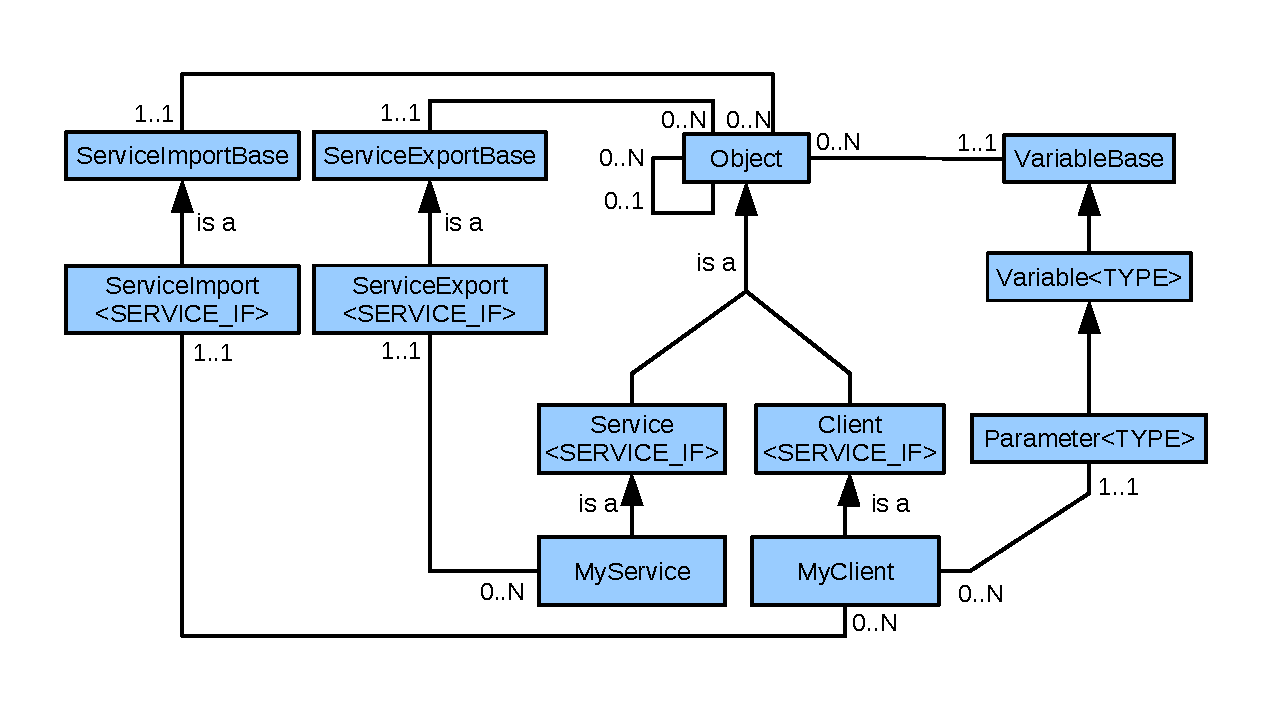
\includegraphics[width=\textwidth]{tms320c3x/fig_object_hierarchy.pdf}
	\end{center}
	\caption{Service/Client/Run-time Parameters Object hierarchy.}
	\label{fig:tms320c3x_object_hierarchy}
\end{figure}

\subsubsection{Building a service graph}
\label{tms320c3x_building_a_service_graph}

Using services implies building a service graph.
For instance, consider that the client is a loader, and the service is a memory.
The programmer creates objects \texttt{loader} and \texttt{memory}, see Figure~\ref{fig:tms320c3x_service_instanciation}.

\begin{figure}[h]
  \begin{center}
    \input{tms320c3x/service_instanciation}
    \caption{\label{fig:tms320c3x_service_instanciation} Client/Service instantiation.}
  \end{center}
\end{figure}

Object \texttt{loader} is a client because it needs a service (reading/writing in memory) from object \texttt{memory} to load the program.
\texttt{loader} has a member \texttt{import} named \texttt{memory\_import} whereas \texttt{memory} object has a member \texttt{export} named \texttt{memory\_export}.
The programmer connects the loader to the memory using \texttt{loader.memory\_import} and \texttt{memory.memory\_export}, see Figure~\ref{fig:tms320c3x_service_connection}.

\begin{figure}[h]
  \begin{center}
    \input{tms320c3x/service_connection}
    \caption{\label{fig:tms320c3x_service_connection} Import/Export connection.}
  \end{center}
\end{figure}

Once \hfill the \hfill programmer \hfill has \hfill created \hfill a \hfill service \hfill graph, \hfill he \hfill must \hfill perform \hfill a \hfill call \hfill to \hfill \texttt{ServiceManager::Setup()}.
\texttt{ServiceManager::Setup()} returns \texttt{true} if setup of each service and client in the graph has been successful, otherwise it returns \texttt{false}.

\subsubsection{Designing a service}

A service is a C++ object inheriting from template class \texttt{Service<SERVICE\_INTERFACE>} \ding{202}, see Figure~\ref{fig:tms320c3x_simple_service}.
\texttt{SERVICE\_INTERFACE} is a C++ abstract class defining the virtual methods implemented by the service.
To export its interface, a service must have a member of type \texttt{ServiceExport<SERVICE\_INTERFACE>} \ding{203}.
For normalization purposes, the service constructor should only take two parameters \ding{204}: the service name and the pointer to the parent (a container service).
The pointer to the parent is \texttt{null} if the service is a top level service (no parent).
The base \texttt{Object} constructor \ding{205} and the base \texttt{Service} constructor \ding{206} must be called with the name and the pointer to the parent.
\texttt{ServiceExport} member constructor must be called with the export name and a pointer to the owner, i.e. the service itself \ding{207}.

\begin{figure}[h]
  \begin{center}
    \input{tms320c3x/simple_service}
    \caption{\label{fig:tms320c3x_simple_service} Simple service.}
  \end{center}
\end{figure}

\subsubsection{Designing a client}

A client is a C++ object inheriting from template class \texttt{Client<SERVICE\_INTERFACE>} \ding{202}, see Figure~\ref{fig:tms320c3x_simple_client}.
\texttt{SERVICE\_INTERFACE} is a C++ abstract class defining the virtual methods implemented by the service the client can call.
To import an interface, a client must have a member of type \texttt{ServiceImport<SERVICE\_INTERFACE>} \ding{203}.
For normalization purposes, the client constructor should only take two parameters \ding{204}: the client name and the pointer to the parent (a container client).
The pointer to the parent is \texttt{null} if the client is a top level client (no parent).
The base \texttt{Object} constructor \ding{205} and the base \texttt{Client} constructor \ding{206} must be called with the name and the pointer to the parent.
\texttt{ServiceImport} member constructor must be called with the import name and a pointer to the owner, i.e. the client itself \ding{207}.


\begin{figure}[h]
  \begin{center}
    \input{tms320c3x/simple_client}
    \caption{\label{fig:tms320c3x_simple_client} Simple client.}
  \end{center}
\end{figure}

\subsubsection{Run-time parameters}

Run-time parameterization can be added to a service or a client.
``Run-time parameterization'' means that the service and/or client can be reconfigured at run-time.
It is opposed to ``Static parameterization'' or ``template parameterization'' which allows configuring a service and/or client at compilation-time.
To expose a member variable as a run-time parameter, a client/service must have a member variable of type \texttt{Parameter<TYPE>}, where \texttt{TYPE} is the C++ type of the exposed member variable, see Figure~\ref{fig:tms320c3x_run_time_parameter}.
Multiple \texttt{Parameter} variables with different \texttt{TYPE}s can be defined within a client/service.
Consider that a service would expose a member variable \texttt{x} \ding{202}.
An instance of class \texttt{Parameter} is defined as a member of the service \ding{203}. 
The parameter is bound to the exposed variable \ding{204} in the service/client constructor.

\begin{figure}[h]
  \begin{center}
    \input{tms320c3x/run_time_parameter}
    \caption{\label{fig:tms320c3x_run_time_parameter} Exposing a service/client member variable as a run-time parameter.}
  \end{center}
\end{figure}

\subsubsection{Setup Order}

As explained in section~\ref{tms320c3x_building_a_service_graph}, method \texttt{Setup} of class \texttt{ServiceManager} calls all \texttt{Setup} methods in the simulator. 
A problem may occur if setup order is important.
For instance, consider two services: service \texttt{A} and \texttt{B}. 
\texttt{A::Setup()} uses service \texttt{B}.
A correct setup order consist to first setup service \texttt{B} and then service \texttt{A}.
To solve such setup dependency, programmer should call method \texttt{ServiceExportBase::SetupDependsOn} (e.g. in the class constructor) so that the service manager can ensure correct setup order.
If the service manager finds a cyclic dependency, \texttt{ServiceManager::Setup()} fails: it generally means that clients and services have been badly designed.

\newpage
\subsection{Service Interfaces}
\label{tms320c3x_interfaces}

All service interfaces are declared in namespace \texttt{unisim::service::interfaces} and located in directory \texttt{unisim/service/interfaces}.

\subsubsection{Memory Interfaces}

These interfaces allow reading/writing from/to memory space. The memory interfaces comes in two flavors:
\begin{itemize}
\item Non-intrusive memory access (\texttt{unisim::service::interfaces::Memory}): It should not affect timing and data placement (e.g. in caches and TLBs).
\item Intrusive memory access (\texttt{unisim::service::interfaces::MemoryInjection}): It can affect timing and data placement.
\end{itemize}

\noindent The two C++ interfaces are:

\begin{center}
	\input{tms320c3x/memory_interface}
\end{center}

\begin{center}
	\input{tms320c3x/memory_injection_interface}
\end{center}

\noindent The arguments to methods \texttt{ReadMemory}, \texttt{InjectReadMemory}, \texttt{WriteMemory}, \texttt{InjectWriteMemory} are:
\begin{itemize}
\item \texttt{addr}: the starting address of the data transfer between the memory and the buffer
\item \texttt{buffer}: a pointer to the buffer of bytes
\item \texttt{size}: the length in bytes to transfer between the memory and the buffer
\end{itemize}

\subsubsection{Debugging Interfaces}

These interfaces are intended for the connection of the simulation components (e.g. CPU, memory, devices, \ldots) with a debugger (e.g. inline-debugger, GDB server, \ldots).

\textbf{Instruction disassembly}. CPU components provide a disassembly capability of the instruction set using the \texttt{unisim::service::interfaces::Disassembly} interface for the debbuger.

\begin{center}
	\input{tms320c3x/disassembly_interface}
\end{center}

\noindent Method \texttt{Disasm} arguments are:
\begin{itemize}
\item \texttt{addr}: the byte address of the instruction to disassemble
\item \texttt{next\_addr}: the byte address of the next instruction
\end{itemize}
\noindent and returns a string with the disassembly of the instruction.

\textbf{Register access}. A CPU or a device provides an access to its registers using the \texttt{unisim::service::interfaces::Registers} interface for the debugger.

\begin{center}
	\input{tms320c3x/registers_interface}
\end{center}

\noindent Method \texttt{GetRegister} arguments are:
\begin{itemize}
\item \texttt{name}: the name of the register to retrieve the register interface
\end{itemize}
\noindent and returns a pointer to an \texttt{unisim::util::debug::Register} interface.

\begin{center}
	\input{tms320c3x/register_interface}
\end{center}

\noindent Method \texttt{GetName} returns the register name.
\noindent Method \texttt{GetValue} fills in a buffer with the register value.
\noindent Method \texttt{SetValue} sets the register value from a buffer.
\noindent Method \texttt{GetSize} returns the register size in bytes.

\textbf{Step by step execution}. A simulation component (e.g. a CPU) leaves control to a debugger with the \texttt{unisim::service::interfaces::DebugYielding} interface.

\begin{center}
	\input{tms320c3x/debug_control_interface}
\end{center}

Method \texttt{FetchDebugCommand} takes the current program counter as argument and returns a command for the simulation component: either finish the simulation or execute one instruction.

\textbf{Monitoring memory accesses}. An instrumented simulation component provides a memory access trace using the \texttt{unisim::service::interfaces::MemoryAccessReporting} interface.
Such memory trace is useful for a debugger to monitor memory access.

\begin{center}
	\input{tms320c3x/memory_access_reporting_interface}
\end{center}

Method \texttt{ReportMemoryAccess} takes as arguments the memory access type (either read or write), the memory type (either data or instruction memory), the address of the access, and the size of the memory access.
Method \texttt{ReportFinishedInstruction} takes as argument the address of next instruction to be executed.

\textbf{Trap reporting}. An instrumented simulation component informs a debugger about an important event using the \texttt{unisim::service::interfaces::TrapReporting} interface.
Such event is useful for a debugger to pause simulation when such event occurs.

\begin{center}
	\input{tms320c3x/trap_reporting_interface}
\end{center}

Method \texttt{ReportTrap} takes no arguments.

\textbf{Symbol}. A service (e.g. a loader) provides lookup to the symbol table using the \texttt{unisim::service::interfaces::SymbolTableLookup} interface.
This interface is useful for translating addresses to symbol names, and vice-versa.

\begin{center}
	\input{tms320c3x/symbol_table_lookup_interface}
\end{center}

\textbf{Efficient instrumentation.} To limit the impact on simulation performance of memory access instrumentation in the simulation components, such instrumentation can be enabled or disabled at run-time using interface \texttt{unisim::service::interfaces::MemoryAccessReportingControl}.

\begin{center}
	\input{tms320c3x/memory_access_reporting_control_interface}
\end{center}

\subsubsection{Loader Interface}

This interface provides basic informations about the loaded program.

\begin{center}
	\input{tms320c3x/loader_interface}
\end{center}

\subsubsection{Time Interface}

This interface provides the current simulation time of the component using it.


\begin{center}
	\input{tms320c3x/time_interface}
\end{center}

\subsubsection{TI C I/O Interface}

An instrumented TMS320C3X instruction set simulator provides a trace of \texttt{SWI} instructions using the \texttt{unisim::service::interfaces::ti\_c\_io} interface.
This interface is useful for the TI C I/O service to capture target program I/Os and translate them to host I/Os.

\begin{center}
	\input{tms320c3x/ti_c_io_interface}
\end{center}

\newpage
\subsection{Services}
\subsubsection{COFF loader service}
\label{tms320c3x_coff_loader}

This service provides UNISIM TMS320C3X simulator with a support for TI COFF v0, v1, and v2 binary files  either with little-endian or big-endian headers (see TMS320C3x/C4x Assembly Language Tools User’s Guide, Appendix A). 
The COFF loader service loads the programs into memory while setup (simulator initialization).
The loader can interpret \texttt{.cinit} section if option \texttt{-cr} of TI C cross-compiler has been used while building the target program (see \textit{TMS320C3x/C4x Optimizing C Compiler User’s Guide}, section 4.8.1: \textit{Autoinitialization of variables and constants}).
To configure the COFF loader service see Section~\ref{tms320c3x_configuration}.
The source code of COFF loader service is located in directory \texttt{unisim/service/loader/coff\_loader}.
\noindent The table below summarizes the COFF Loader service API:

\begin{center}
	\tablehead{\hline}
	\tabletail{\hline}
	\begin{supertabular}{|p{7.5cm}|p{7.5cm}|}
		\hline
		\multicolumn{2}{|l|}{\textbf{\Large Service COFF Loader}}\\
		\hline
		\multicolumn{1}{|p{7.5cm}}{\textbf{Class Name:} \newline \texttt{unisim::service::loader::coff\_loader}\newline$\hookrightarrow$\texttt{::CoffLoader}} & \multicolumn{1}{p{7.5cm}|}{\textbf{Header:} \newline \texttt{unisim/service/loader/coff\_loader}\newline$\hookrightarrow$\texttt{/coff\_loader.hh}}\\
		\multicolumn{2}{|l|}{}\\
		\multicolumn{2}{|p{15cm}|}{\textbf{Description:} \newline The COFF loader service allows to load a COFF binary program into a memory and fill a symbol table. The loader also provides information about the loaded file such as the code and data locations (base address and size). The COFF loader loads the program during setup.}\\
		\hline
		\hline
		\multicolumn{2}{|c|}{\textbf{\large Template Parameters}}\\
		\hline
		\multicolumn{1}{|p{7.5cm}}{\textbf{Name:} \texttt{MEMORY\_ADDR}} & \multicolumn{1}{p{7.5cm}|}{\textbf{Type:} \texttt{class}}\\
		\multicolumn{2}{|p{15cm}|}{\textbf{Default value:} \texttt{none}}\\
		\multicolumn{2}{|l|}{}\\
		\multicolumn{2}{|p{15cm}|}{\textbf{Description:} \newline This is the C++ type of a memory address (e.g. \texttt{uint32\_t} or \texttt{uint64\_t}).}\\
		\hline
		\hline
		\multicolumn{2}{|c|}{\textbf{\large Run-Time Parameters}}\\
		\hline
		\multicolumn{1}{|p{7.5cm}}{\textbf{Name:} \texttt{filename}} & \multicolumn{1}{p{7.5cm}|}{\textbf{Type:} \texttt{string}}\\
		\multicolumn{2}{|p{15cm}|}{\textbf{Default value:} empty string}\\
		\multicolumn{2}{|l|}{}\\
		\multicolumn{2}{|p{15cm}|}{\textbf{Description:} \newline The COFF file name to load into the connected memory.}\\
		\hline
		\hline
		\multicolumn{1}{|p{7.5cm}}{\textbf{Name:} \texttt{dump-headers}} & \multicolumn{1}{p{7.5cm}|}{\textbf{Type:} \texttt{boolean}}\\
		\multicolumn{2}{|p{15cm}|}{\textbf{Default value:} false}\\
		\multicolumn{2}{|l|}{}\\
		\multicolumn{2}{|p{15cm}|}{\textbf{Description:} \newline If true this parameter makes the COFF loader print the file headers on the screen (file header, section headers, symbol table \ldots) while loading the program.}\\
		\hline
		\multicolumn{2}{|c|}{\textbf{\large Service Exports}}\\
		\hline
		\multicolumn{1}{|p{7.5cm}}{\textbf{Name:} \texttt{logger\_export}} & \multicolumn{1}{p{7.5cm}|}{\textbf{Interface:} \newline \texttt{unisim::service::interfaces::} \newline$\hookrightarrow$\texttt{Loader<MEMORY\_ADDR>}}\\
		\multicolumn{2}{|l|}{}\\
		\multicolumn{2}{|p{15cm}|}{\textbf{Description:} \newline The COFF loader provides information about the code and data location through this export.}\\
		\hline
		\multicolumn{1}{|p{7.5cm}}{\textbf{Name:} \texttt{symbol\_table\_lookup\_export}} & \multicolumn{1}{p{7.5cm}|}{\textbf{Interface:} \newline \texttt{unisim::service::interfaces::} \newline$\hookrightarrow$\texttt{SymbolTableLookup<MEMORY\_ADDR>}}\\
		\multicolumn{2}{|l|}{}\\
		\multicolumn{2}{|p{15cm}|}{\textbf{Description:} \newline The COFF loader provides symbol lookup through this export.}\\
		\hline
		\hline
		\multicolumn{2}{|c|}{\textbf{\large Service Imports}}\\
		\hline
		\multicolumn{1}{|p{7.5cm}}{\textbf{Name:} \texttt{memory\_import} \newline \textbf{Mandatory connected:} no} & \multicolumn{1}{p{7.5cm}|}{\textbf{Interface:} \newline \texttt{unisim::service::interfaces::} \newline$\hookrightarrow$\texttt{Memory<uint32\_t>}}\\
		\multicolumn{2}{|l|}{}\\
		\multicolumn{2}{|p{15cm}|}{\textbf{Description:} \newline The COFF loader accesses to the memory through this import.}\\
		\hline
	\end{supertabular}
\end{center}

\newpage
\subsubsection{TI C I/O service}
\label{tms320c3x_ti_c_io}

This service provides low level I/O (open, read, write, close, \ldots) support on the host machine for target programs.
The TI Run-time support libraries (\texttt{RTS*.lib}) implement a software stack for standard C I/Os (see \textit{TMS320C3x/C4x Optimizing C Compiler User’s Guide} (SPRU034H, June 1998), Appendix B).
A development board debugger captures target program I/Os at \texttt{C\$\$IO\$\$}.
The Run-time support library puts the I/Os in a communication buffer (\texttt{\_\_CIOBUF\_}) that the development board debugger translates to host I/Os.
The debugger also captures target program termination at \texttt{C\$\$EXIT}.
The UNISIM TI C I/O service captures and translates target program I/Os and termination in the same manner as a development board built-in debugger.
To configure the TI C I/O service see Section~\ref{tms320c3x_configuration}.
The source code of the COFF loader service is located in directory \texttt{unisim/service/os/ti\_c\_io}.
\noindent The table below summarizes the TI C I/O service API:

\begin{center}
	\tablehead{\hline}
	\tabletail{\hline}
	\begin{supertabular}{|p{7.5cm}|p{7.5cm}|}
		\hline
		\multicolumn{2}{|l|}{\textbf{\Large Service TI C I/O}}\\
		\hline
		\multicolumn{1}{|p{7.5cm}}{\textbf{Class Name:} \newline \texttt{unisim::service::os::ti\_c\_io}\newline$\hookrightarrow$\texttt{::TI\_C\_IO}} & \multicolumn{1}{p{7.5cm}|}{\textbf{Header:} \newline \texttt{unisim/service/os/ti\_c\_io}\newline$\hookrightarrow$\texttt{/ti\_c\_io.hh}}\\
		\multicolumn{2}{|l|}{}\\
		\multicolumn{2}{|p{15cm}|}{\textbf{Description:} \newline The TI C I/O service provides low level I/O (open, read, write, close, \ldots) support on the host machine for target programs.}\\
		\hline
		\hline
		\multicolumn{2}{|c|}{\textbf{\large Template Parameters}}\\
		\hline
		\multicolumn{1}{|p{7.5cm}}{\textbf{Name:} \texttt{MEMORY\_ADDR}} & \multicolumn{1}{p{7.5cm}|}{\textbf{Type:} \texttt{class}}\\
		\multicolumn{2}{|p{15cm}|}{\textbf{Default value:} \texttt{none}}\\
		\multicolumn{2}{|l|}{}\\
		\multicolumn{2}{|p{15cm}|}{\textbf{Description:} \newline This is the C++ type of a memory address (e.g. uint32\_t or uint64\_t).}\\
		\hline
		\hline
		\multicolumn{2}{|c|}{\textbf{\large Run-Time Parameters}}\\
		\hline
		\multicolumn{1}{|p{7.5cm}}{\textbf{Name:} \texttt{ti\_c\_io.enable}} & \multicolumn{1}{p{7.5cm}|}{\textbf{Type:} \texttt{bool}}\\
		\multicolumn{2}{|p{15cm}|}{\textbf{Default value:} \texttt{false}}\\
		\multicolumn{2}{|l|}{}\\
		\multicolumn{2}{|p{15cm}|}{\textbf{Description:} \newline Enable/disable TI C I/O support.}\\
		\hline
		\multicolumn{1}{|p{7.5cm}}{\textbf{Name:} \texttt{ti-c-io.warning-as-error}} & \multicolumn{1}{p{7.5cm}|}{\textbf{Type:} \texttt{bool}}\\
		\multicolumn{2}{|p{15cm}|}{\textbf{Default value:} \texttt{false}}\\
		\multicolumn{2}{|l|}{}\\
		\multicolumn{2}{|p{15cm}|}{\textbf{Description:} \newline Whether Warnings are considered as error or not.}\\
		\hline
		\multicolumn{1}{|p{7.5cm}}{\textbf{Name:} \texttt{ti-c-io.pc-register-name}} & \multicolumn{1}{p{7.5cm}|}{\textbf{Type:} \texttt{string}}\\
		\multicolumn{2}{|p{15cm}|}{\textbf{Default value:} \texttt{"PC"}}\\
		\multicolumn{2}{|l|}{}\\
		\multicolumn{2}{|p{15cm}|}{\textbf{Description:} \newline Name of the CPU program counter register.}\\
		\hline
		\multicolumn{1}{|p{7.5cm}}{\textbf{Name:} \texttt{ti-c-io.c-io-buffer-symbol-name}} & \multicolumn{1}{p{7.5cm}|}{\textbf{Type:} \texttt{string}}\\
		\multicolumn{2}{|p{15cm}|}{\textbf{Default value:} \texttt{"\_\_CIOBUF\_"}}\\
		\multicolumn{2}{|l|}{}\\
		\multicolumn{2}{|p{15cm}|}{\textbf{Description:} \newline C I/O buffer symbol name.}\\
		\hline
		\multicolumn{1}{|p{7.5cm}}{\textbf{Name:} \texttt{ti-c-io.c-io-breakpoint-}\newline$\hookrightarrow$\texttt{symbol-name}} & \multicolumn{1}{p{7.5cm}|}{\textbf{Type:} \texttt{string}}\\
		\multicolumn{2}{|p{15cm}|}{\textbf{Default value:} \texttt{"C\$\$IO\$\$"}}\\
		\multicolumn{2}{|l|}{}\\
		\multicolumn{2}{|p{15cm}|}{\textbf{Description:} \newline C I/O breakpoint symbol name. The TI C I/O service installs a \texttt{SWI} instruction at this point to capture target program I/O.}\\
		\hline
		\multicolumn{1}{|p{7.5cm}}{\textbf{Name:} \texttt{ti-c-io.c-exit-breakpoint-}\newline$\hookrightarrow$\texttt{symbol-name}} & \multicolumn{1}{p{7.5cm}|}{\textbf{Type:} \texttt{string}}\\
		\multicolumn{2}{|p{15cm}|}{\textbf{Default value:} \texttt{"C\$\$EXIT"}}\\
		\multicolumn{2}{|l|}{}\\
		\multicolumn{2}{|p{15cm}|}{\textbf{Description:} \newline C EXIT breakpoint symbol name. The TI C I/O service installs a \texttt{SWI} instruction at this point to capture target program exit.}\\
		\hline
		\multicolumn{1}{|p{7.5cm}}{\textbf{Name:} \texttt{ti-c-io.verbose-all}} & \multicolumn{1}{p{7.5cm}|}{\textbf{Type:} \texttt{bool}}\\
		\multicolumn{2}{|p{15cm}|}{\textbf{Default value:} \texttt{false}}\\
		\multicolumn{2}{|l|}{}\\
		\multicolumn{2}{|p{15cm}|}{\textbf{Description:} \newline Globally enable/disable verbosity of TI C I/O service.}\\
		\hline
		\multicolumn{1}{|p{7.5cm}}{\textbf{Name:} \texttt{ti-c-io.verbose-io}} & \multicolumn{1}{p{7.5cm}|}{\textbf{Type:} \texttt{bool}}\\
		\multicolumn{2}{|p{15cm}|}{\textbf{Default value:} \texttt{false}}\\
		\multicolumn{2}{|l|}{}\\
		\multicolumn{2}{|p{15cm}|}{\textbf{Description:} \newline Enable/disable verbosity of TI C I/O service while performing I/Os.}\\
		\hline
		\multicolumn{1}{|p{7.5cm}}{\textbf{Name:} \texttt{ti-c-io.verbose-setup}} & \multicolumn{1}{p{7.5cm}|}{\textbf{Type:} \texttt{bool}}\\
		\multicolumn{2}{|p{15cm}|}{\textbf{Default value:} \texttt{false}}\\
		\multicolumn{2}{|l|}{}\\
		\multicolumn{2}{|p{15cm}|}{\textbf{Description:} \newline Enable/disable verbosity of TI C I/O service while setup.}\\
		\hline
		\hline
		\multicolumn{2}{|c|}{\textbf{\large Service Exports}}\\
		\hline
		\multicolumn{1}{|p{7.5cm}}{\textbf{Name:} \texttt{ti\_c\_io\_export}} & \multicolumn{1}{p{7.5cm}|}{\textbf{Interface:} \newline \texttt{unisim::interfaces::} \newline$\hookrightarrow$\texttt{TI\_C\_IO<MEMORY\_ADDR>}}\\
		\multicolumn{2}{|l|}{}\\
		\multicolumn{2}{|p{15cm}|}{\textbf{Description:} \newline The TI C I/O provides target to host I/O translation through this service export.}\\
		\hline
		\hline
		\multicolumn{2}{|c|}{\textbf{\large Service Imports}}\\
		\hline
		\multicolumn{1}{|p{7.5cm}}{\textbf{Name:} \texttt{memory\_import}} & \multicolumn{1}{p{7.5cm}|}{\textbf{Interface:} \newline \texttt{unisim::service::interfaces::} \newline$\hookrightarrow$\texttt{Memory<MEMORY\_ADDR>}}\\
		\multicolumn{2}{|p{15cm}|}{\textbf{Mandatory connected:} no}\\
		\multicolumn{2}{|l|}{}\\
		\multicolumn{2}{|p{15cm}|}{\textbf{Description:} \newline The TI C I/O service accesses to the memory while setup through this import. While in setup it installs two \texttt{SWI} instructions to capture both target I/O and program exit.}\\
		\hline
		\multicolumn{1}{|p{7.5cm}}{\textbf{Name:} \texttt{memory\_injection\_import}} & \multicolumn{1}{p{7.5cm}|}{\textbf{Interface:} \newline \texttt{unisim::service::interfaces::} \newline$\hookrightarrow$\texttt{MemoryInjection<MEMORY\_ADDR>}}\\
		\multicolumn{2}{|p{15cm}|}{\textbf{Mandatory connected:} no}\\
		\multicolumn{2}{|l|}{}\\
		\multicolumn{2}{|p{15cm}|}{\textbf{Description:} \newline The TI C I/O service accesses to the memory while simulation through this import. It accesses to the I/O buffer in the target program memory and then interprete the content of this buffer to translate target program I/Os to host I/Os.}\\
		\hline
		\multicolumn{1}{|p{7.5cm}}{\textbf{Name:} \texttt{registers\_import} \newline \textbf{Mandatory connected:} yes} & \multicolumn{1}{p{7.5cm}|}{\textbf{Interface:} \newline \texttt{unisim::service::interfaces} \newline$\hookrightarrow$\texttt{::Registers}}\\
		\multicolumn{2}{|l|}{}\\
		\multicolumn{2}{|p{15cm}|}{\textbf{Description:} \newline This service import should be connected to a CPU module. The TI C I/O service calls method \texttt{GetRegister} through this service import to get an interface to the CPU registers. The TI C I/O service uses methods \texttt{GetName}, \texttt{GetValue}, \texttt{GetSize} and \texttt{SetValue} of that interface to access to CPU registers. This import is mainly used to get the current PC, so that the TI C I/O service can distinguish target program I/Os from target program exit.}\\
		\hline
		\multicolumn{1}{|p{7.5cm}}{\textbf{Name:} \texttt{symbol\_table\_lookup\_import} \newline \textbf{Mandatory connected:} yes} & \multicolumn{1}{p{7.5cm}|}{\textbf{Interface:} \newline \texttt{unisim::service::interfaces} \newline$\hookrightarrow$\texttt{::SymbolTableLookup<MEMORY\_ADDR>}}\\
		\multicolumn{2}{|l|}{}\\
		\multicolumn{2}{|p{15cm}|}{\textbf{Description:} \newline The TI C I/O service uses this service import to get the address of the breakpoints and I/O buffer from their symbol name.}\\
		\hline
	\end{supertabular}
\end{center}

\newpage
\subsubsection{Inline debugger}
\label{tms320c3x_inline_debugger}

The inline debugger service is a built-in debugger with a text-based user interface, see~\ref{tms320c3x_inline_debug}. 
It provides instruction level debugging of the target program.
\noindent Table below summarizes the inline debugger service API:

\begin{center}
	\tablehead{\hline}
	\tabletail{\hline}
	\begin{supertabular}{|p{7.5cm}|p{7.5cm}|}
		\hline
		\multicolumn{2}{|l|}{\textbf{\Large Service Inline Debugger}}\\
		\hline
		\multicolumn{1}{|p{7.5cm}}{\textbf{Class Name:} \newline \texttt{unisim::service::debug}\newline$\hookrightarrow$\texttt{::inline\_debugger::InlineDebugger}} & \multicolumn{1}{p{7.5cm}|}{\textbf{Header:} \newline \texttt{unisim/service/debug}\newline$\hookrightarrow$\texttt{/inline\_debugger/inline\_debugger.hh}}\\
		\multicolumn{2}{|l|}{}\\
		\multicolumn{2}{|p{15cm}|}{\textbf{Description:} \newline The inline debugger service provides a simple text-based interface to interactively debug a target application running on a CPU module for the user. The debug is at the instruction level. The inline debugger may be connected to a CPU module.}\\
		\hline
		\hline
		\multicolumn{2}{|c|}{\textbf{\large Template Parameters}}\\
		\hline
		\multicolumn{1}{|p{7.5cm}}{\textbf{Name:} \texttt{ADDRESS}} & \multicolumn{1}{p{7.5cm}|}{\textbf{Type:} \texttt{class}}\\
		\multicolumn{2}{|p{15cm}|}{\textbf{Default value:} none}\\
		\multicolumn{2}{|l|}{}\\
		\multicolumn{2}{|p{15cm}|}{\textbf{Description:} \newline This is the C++ type of a memory address (e.g. uint32\_t or uint64\_t).}\\
		\hline
		\hline
		\multicolumn{2}{|c|}{\textbf{\large Run-time parameters}}\\
		\hline
		\multicolumn{1}{|p{7.5cm}}{\textbf{Name:} \texttt{inline-debugger.memory-atom-size}} & \multicolumn{1}{p{7.5cm}|}{\textbf{Type:} \texttt{unsigned integer}}\\
		\multicolumn{2}{|p{15cm}|}{\textbf{Default value:} \texttt{1}}\\
		\multicolumn{2}{|l|}{}\\
		\multicolumn{2}{|p{15cm}|}{\textbf{Description:} \newline Size of the smallest addressable element in memory.}\\
		\hline
		\hline
		\multicolumn{2}{|c|}{\textbf{\large Service Exports}}\\
		\hline
		\multicolumn{1}{|p{7.5cm}}{\textbf{Name:} \texttt{debug\_control\_export}} & \multicolumn{1}{p{7.5cm}|}{\textbf{Interface:} \newline \texttt{unisim::service::interfaces} \newline$\hookrightarrow$\texttt{::DebugControl<ADDRESS>}}\\
		\multicolumn{2}{|l|}{}\\
		\multicolumn{2}{|p{15cm}|}{\textbf{Description:} \newline This service export should be connected to a CPU module. The CPU module calls method \texttt{FetchDebugCommand} through its service import to leave control to the debugger and fetch a new debug command.}\\
		\hline
		\multicolumn{1}{|p{7.5cm}}{\textbf{Name:} \texttt{memory\_access\_reporting\_export}} & \multicolumn{1}{p{7.5cm}|}{\textbf{Interface:} \newline \texttt{unisim::service::interfaces} \newline$\hookrightarrow$\texttt{MemoryAccessReporting<ADDRESS>}}\\
		\multicolumn{2}{|l|}{}\\
		\multicolumn{2}{|p{15cm}|}{\textbf{Description:} \newline This service export should be connected to a CPU module. The CPU module calls methods \texttt{ReportMemoryAccess} and \texttt{ReportFinishedInstruction} through its service import. This allows the debugger to spy memory accesses and thus handle breakpoints and watchpoints.}\\
		\hline
		\multicolumn{1}{|p{7.5cm}}{\textbf{Name:} \texttt{trap\_reporting\_export}} & \multicolumn{1}{p{7.5cm}|}{\textbf{Interface:} \newline \texttt{unisim::service::interfaces} \newline$\hookrightarrow$\texttt{::TrapReporting}}\\
		\multicolumn{2}{|l|}{}\\
		\multicolumn{2}{|p{15cm}|}{\textbf{Description:} \newline This service export should be connected to a CPU module. A CPU module calls method \texttt{ReportTrap} through its service import. This allows the debugger to break execution on the simulated CPU once a trap condition is detected by the CPU module.}\\
		\hline
		\hline
		\multicolumn{2}{|c|}{\textbf{\large Service Imports}}\\
		\hline
		\multicolumn{1}{|p{7.5cm}}{\textbf{Name:} \texttt{disasm\_import} \newline \textbf{Mandatory connected:} yes} & \multicolumn{1}{p{7.5cm}|}{\textbf{Interface:} \newline \texttt{unisim::service::interfaces} \newline$\hookrightarrow$\texttt{::Disassembly<ADDRESS>}}\\
		\multicolumn{2}{|l|}{}\\
		\multicolumn{2}{|p{15cm}|}{\textbf{Description:} \newline This service import should be connected to a CPU module. The CPU module should implement method \texttt{Disassemble} which provides disassembling of the instructions for the debugger.}\\
		\hline
		\multicolumn{1}{|p{7.5cm}}{\textbf{Name:} \texttt{memory\_import} \newline \textbf{Mandatory connected:} yes} & \multicolumn{1}{p{7.5cm}|}{\textbf{Interface:} \newline \texttt{unisim::service::interfaces} \newline$\hookrightarrow$\texttt{::Memory<ADDRESS>}}\\
		\multicolumn{2}{|l|}{}\\
		\multicolumn{2}{|p{15cm}|}{\textbf{Description:} \newline This service import should be connected to a CPU or a memory module. The debugger uses this service import to access to memory using methods \texttt{ReadMemory} and \texttt{WriteMemory}.}\\
		\hline
		\multicolumn{1}{|p{7.5cm}}{\textbf{Name:} \texttt{memory\_access\_reporting\newline$\hookrightarrow$\_control\_import} \newline \textbf{Mandatory connected:} no} & \multicolumn{1}{p{7.5cm}|}{\textbf{Interface:} \newline \texttt{unisim::service::interfaces} \newline$\hookrightarrow$\texttt{::MemoryAccessReportingControl}}\\
		\multicolumn{2}{|l|}{}\\
		\multicolumn{2}{|p{15cm}|}{\textbf{Description:} \newline This service import should be connected to a CPU module. The debugger calls methods \texttt{RequiresMemoryAccessReporting} and \texttt{RequiresFinishedInstructionReporting} through this service import to enable/disable memory access reporting from the CPU module.}\\
		\hline
		\multicolumn{1}{|p{7.5cm}}{\textbf{Name:} \texttt{registers\_import} \newline \textbf{Mandatory connected:} yes} & \multicolumn{1}{p{7.5cm}|}{\textbf{Interface:} \newline \texttt{unisim::service::interfaces} \newline$\hookrightarrow$\texttt{::Registers}}\\
		\multicolumn{2}{|l|}{}\\
		\multicolumn{2}{|p{15cm}|}{\textbf{Description:} \newline This service import should be connected to a CPU module. The debugger calls method \texttt{GetRegister} through this service import to get an interface to the CPU registers. The debugger uses methods \texttt{GetName}, \texttt{GetValue}, \texttt{GetSize} and \texttt{SetValue} of that interface to access to CPU registers.}\\
		\hline
		\multicolumn{1}{|p{7.5cm}}{\textbf{Name:} \texttt{symbol\_table\_lookup\_import} \newline \textbf{Mandatory connected:} no} & \multicolumn{1}{p{7.5cm}|}{\textbf{Interface:} \newline \texttt{unisim::service::interfaces} \newline$\hookrightarrow$\texttt{::SymbolTableLookup}}\\
		\multicolumn{2}{|l|}{}\\
		\multicolumn{2}{|p{15cm}|}{\textbf{Description:} \newline This service import should be connected to a symbol table. The debugger calls method \texttt{FindSymbol}, \texttt{FindSymbolByAddr}, \texttt{FindSymbolByName} through this service import to translate addresses to symbols and vice-versa.}\\
		\hline
	\end{supertabular}
\end{center}

\subsubsection{GDB server}
\label{tms320c3x_gdb_server}

The GDB server service emulates the GDB remote serial protocol over TCP/IP (see \textit{Debugging with GDB}, Appendix D. \textit{GDB Remote serial protocol}), so that a GDB client can connect to the simulator and debug the target program as if it were run on the real hardware.
This service uses an architecture XML description file defined by the \texttt{architecture-description-filename} run-time parameter (see table below).
A sample configuration file for a dummy \texttt{XYZ} big-endian architecture, with four 32-bit general purpose registers named \texttt{r0}, \texttt{r1}, \texttt{r2}, \texttt{r3} and a program counter named \texttt{pc} would be the following:
\begin{verbatim}
<architecture name="XYZ" endian="big">
    <program_counter name="pc"/>
    <register name="r0" size="4"/>
    <register name="r1" size="4"/>
    <register name="r2" size="4"/>
    <register name="r3" size="4"/>
</architecture>
\end{verbatim}

\noindent Table below summarizes the GDB server service API:

\begin{center}
	\tablehead{\hline}
	\tabletail{\hline}
	\begin{supertabular}{|p{7.5cm}|p{7.5cm}|}
		\hline
		\multicolumn{2}{|l|}{\textbf{\Large Service GDB Server}}\\
		\hline
		\multicolumn{1}{|p{7.5cm}}{\textbf{Class Name:} \newline \texttt{unisim::service::debug}\newline$\hookrightarrow$\texttt{::gdb\_server::GDBServer}} & \multicolumn{1}{p{7.5cm}|}{\textbf{Header:} \newline \texttt{unisim/service/debug}\newline$\hookrightarrow$\texttt{/gdb\_server/gdb\_server.hh}}\\
		\multicolumn{2}{|l|}{}\\
		\multicolumn{2}{|p{15cm}|}{\textbf{Description:} \newline The GDB server service allows debugging a software running on a simulated hardware by connecting (over TCP/IP) a GDB client to it (and thus to the simulator). The GDB client can be either the standard text based client (i.e. command \texttt{gdb}), a graphical front-end to GDB (e.g. \texttt{ddd}), or even Eclipse CDT. The GDB server service directly speaks to the GDB serial remote protocol (over TCP/IP), so that a GDB client can connect (over TCP/IP) to the simulator using GDB command \texttt{target remote}. The GDB server service may be connected to a CPU module.}\\
		\hline
		\hline
		\multicolumn{2}{|c|}{\textbf{\large Template Parameters}}\\
		\hline
		\multicolumn{1}{|p{7.5cm}}{\textbf{Name:} \texttt{ADDRESS}} & \multicolumn{1}{p{7.5cm}|}{\textbf{Type:} \texttt{class}}\\
		\multicolumn{2}{|p{15cm}|}{\textbf{Default value:} none}\\
		\multicolumn{2}{|l|}{}\\
		\multicolumn{2}{|p{15cm}|}{\textbf{Description:} \newline This is the C++ type of a memory address (e.g. uint32\_t or uint64\_t).}\\
		\hline
		\hline
		\multicolumn{2}{|c|}{\textbf{\large Run-Time Parameters}}\\
		\hline
		\multicolumn{1}{|p{7.5cm}}{\textbf{Name:} \texttt{tcp-port}} & \multicolumn{1}{p{7.5cm}|}{\textbf{Type:} \texttt{int}}\\
		\multicolumn{2}{|p{15cm}|}{\textbf{Default value:} \texttt{12345}}\\
		\multicolumn{2}{|l|}{}\\
		\multicolumn{2}{|p{15cm}|}{\textbf{Description:} \newline The TCP port used by GDB server service to communicate with the GDB client.}\\
		\hline
		\multicolumn{1}{|p{7.5cm}}{\textbf{Name:} \texttt{architecture-description\newline$\hookrightarrow$-filename}} & \multicolumn{1}{p{7.5cm}|}{\textbf{Type:} \texttt{string}}\\
		\multicolumn{2}{|p{15cm}|}{\textbf{Default value:} empty string}\\
		\multicolumn{2}{|l|}{}\\
		\multicolumn{2}{|p{15cm}|}{\textbf{Description:} \newline The path to the architecture description file that the GDB server service must use. The description file provides retargetability to the GDB server service. The following files brings support of the ARM, PowerPC, TMS320C3X and HCS12X processors to the GDB server service: 
		\begin{itemize}
			\item \texttt{unisim/service/debug/gdb\_server/gdb\_armv4l.xml}
			\item \texttt{unisim/service/debug/gdb\_server/gdb\_armv5b.xml}
			\item \texttt{unisim/service/debug/gdb\_server/gdb\_powerpc.xml}
			\item \texttt{unisim/service/debug/gdb\_server/gdb\_tms320c3x.xml}
			\item \texttt{unisim/service/debug/gdb\_server/gdb\_hcs12x.xml}
		\end{itemize}
		}\\
		\hline
		\hline
		\multicolumn{2}{|c|}{\textbf{\large Service Exports}}\\
		\hline
		\multicolumn{1}{|p{7.5cm}}{\textbf{Name:} \texttt{debug\_control\_export}} & \multicolumn{1}{p{7.5cm}|}{\textbf{Interface:} \newline \texttt{unisim::service::interfaces} \newline$\hookrightarrow$\texttt{::DebugControl<ADDRESS>}}\\
		\multicolumn{2}{|l|}{}\\
		\multicolumn{2}{|p{15cm}|}{\textbf{Description:} \newline This service export should be connected to a CPU module. The CPU module calls method \texttt{FetchDebugCommand} through its service import to leave control to the debugger and fetch a new debug command.}\\
		\hline
		\multicolumn{1}{|p{7.5cm}}{\textbf{Name:} \texttt{memory\_access\_reporting\_export}} & \multicolumn{1}{p{7.5cm}|}{\textbf{Interface:} \newline \texttt{unisim::service::interfaces} \newline$\hookrightarrow$\texttt{MemoryAccessReporting<ADDRESS>}}\\
		\multicolumn{2}{|l|}{}\\
		\multicolumn{2}{|p{15cm}|}{\textbf{Description:} \newline This service export should be connected to a CPU module. The CPU module calls methods \texttt{ReportMemoryAccess} and \texttt{ReportFinishedInstruction} through its service import. This allows the debugger to spy memory accesses and thus handle breakpoints and watchpoints.}\\
		\hline
		\multicolumn{1}{|p{7.5cm}}{\textbf{Name:} \texttt{trap\_reporting\_export}} & \multicolumn{1}{p{7.5cm}|}{\textbf{Interface:} \newline \texttt{unisim::service::interfaces} \newline$\hookrightarrow$\texttt{::TrapReporting}}\\
		\multicolumn{2}{|l|}{}\\
		\multicolumn{2}{|p{15cm}|}{\textbf{Description:} \newline This service export should be connected to a CPU module. A CPU module calls method \texttt{ReportTrap} through its service import. This allows the debugger to break execution on the simulated CPU when a trap condition is detected by the CPU module.}\\
		\hline
		\hline
		\multicolumn{2}{|c|}{\textbf{\large Service Imports}}\\
		\hline
		\multicolumn{1}{|p{7.5cm}}{\textbf{Name:} \texttt{memory\_import} \newline \textbf{Mandatory connected:} yes} & \multicolumn{1}{p{7.5cm}|}{\textbf{Interface:} \newline \texttt{unisim::service::interfaces} \newline$\hookrightarrow$\texttt{::Memory<ADDRESS>}}\\
		\multicolumn{2}{|l|}{}\\
		\multicolumn{2}{|p{15cm}|}{\textbf{Description:} \newline This service import should be connected to a CPU or a memory module. The debugger uses this service import to access to memory using methods \texttt{ReadMemory} and \texttt{WriteMemory}.}\\
		\hline
		\multicolumn{1}{|p{7.5cm}}{\textbf{Name:} \texttt{memory\_access\_reporting\newline$\hookrightarrow$\_control\_import} \newline \textbf{Mandatory connected:} no} & \multicolumn{1}{p{7.5cm}|}{\textbf{Interface:} \newline \texttt{unisim::service::interfaces} \newline$\hookrightarrow$\texttt{::MemoryAccessReportingControl}}\\
		\multicolumn{2}{|l|}{}\\
		\multicolumn{2}{|p{15cm}|}{\textbf{Description:} \newline This service import should be connected to a CPU module. The debugger calls methods \texttt{RequiresMemoryAccessReporting} and \texttt{RequiresFinishedInstructionReporting} through this service import to enable/disable memory access reporting from the CPU module.}\\
		\hline
		\multicolumn{1}{|p{7.5cm}}{\textbf{Name:} \texttt{registers\_import} \newline \textbf{Mandatory connected:} yes} & \multicolumn{1}{p{7.5cm}|}{\textbf{Interface:} \newline \texttt{unisim::service::interfaces} \newline$\hookrightarrow$\texttt{::Registers}}\\
		\multicolumn{2}{|l|}{}\\
		\multicolumn{2}{|p{15cm}|}{\textbf{Description:} \newline This service import should be connected to a CPU module. The debugger calls method \texttt{GetRegister} through this service import to get an interface to the CPU registers. The debugger uses methods \texttt{GetName}, \texttt{GetValue}, \texttt{GetSize} and \texttt{SetValue} of that interface to access to CPU registers.}\\
		\hline
	\end{supertabular}
\end{center}

\newpage
\subsubsection{Built-in Logger}
\label{tms320c3x_logger}

UNISIM provides you a centralized log system to debug modules and simulators. It should be used to show all debug messages, instead of using the traditional C++ stream output mechanism (\texttt{cerr} and \texttt{cout}). However, as you will see below the UNISIM log system works much like the C++ stream output mechanism.

It provides the following advantages:
\begin{itemize}
\item Categorization: messages can be categorized on information, warning and error messages
\item Atomic messages: messages will not be mixed (something which happens when programming concurrent/parallel systems like UNISIM/SystemC)
\item Multiple outputs: your messages can be written simultaneously to different outputs, for example:
	\begin{itemize}
	\item console (error output or standard output)
	\item raw file
	\item XML formatted file
	\item ...
	\end{itemize}
\item Simple configuration: the log system configuration is integrated to the UNISIM parameter mechanism provided by UNISIM service, see~\ref{tms320c3x_configuration}.
\end{itemize}

To use the UNISIM logger you need to include “unisim/kernel/logger/logger.hh” and declare that you are using the unisim::kernel::logger namespace:

\begin{center}
	\input{tms320c3x/including_logger}
\end{center}

The logger can only be used by UNISIM objects, that is, classes that inherit from \newline
\texttt{unisim::kernel::service::Object}. 
So if you want to use the UNISIM log system your class must inherit from a UNISIM object.

\begin{center}
	\input{tms320c3x/deriving_from_object}
\end{center}

You will need to create a member variable of the \texttt{unisim::kernel::logger::Logger} type. 
And at the construction of your object use its default constructor \newline
\texttt{Logger(const unisim::kernel::service::Object \&obj)}. For example:

\begin{center}
	\input{tms320c3x/binding_logger}
\end{center}

Once you have initialized your member logger variable you can start using it in your class methods.
Basically it works like an standard C++ output stream, with the \texttt{<<} operator. 
However, it requires that you indicate when a message starts and ends, and its category (information, warning or error) with the following keywords:
\begin{itemize}
\item \texttt{DebugInfo} and \texttt{EndDebugInfo} to start and end an information message
\item \texttt{DebugWarning} and \texttt{EndDebugWarning} to start and end a warning message
\item \texttt{DebugError} and \texttt{EndDebugError} to start and end an error message
\end{itemize}

You can use the keyword \texttt{EndDebug} instead of \texttt{EndDebugInfo}, \texttt{EndDebugWarning} or \texttt{EndDebugWarning} to indicate that a message ends.
The log system will automatically decide which kind of message you are ending. 
Between the start and the end of a message you can use the logger as a normal C++ output stream.
Some of examples of its use:
\begin{center}
	\input{tms320c3x/using_logger}
\end{center}

\newpage
\subsection{Utility classes}
\label{tms320c3x_utils}

The utility classes source code is in \texttt{unisim/util}.

\subsubsection{Arithmetic and Logical helper functions}

These functions located in \texttt{unisim/util/arithmetic} implement fast integer arithmetic computations (assembly on i386 machines):
\begin{itemize}
\item Full Adders (8, 16, 32, and 64 bits)
\item Full Substractors (8, 16, 32, and 64 bits)
\item Full Adders with signed saturation (8, 16, 32, and 64 bits)
\item Full Substractors with signed saturation (8, 16, 32, and 64 bits)
\item Specific Adders (e.g. reversed carry propagation adder)
\item Rotates (left, right, through an additional virtual bit, with bit in, with bit out)
\item Logical Shifts (left, right, through an additional virtual bit, with bit in, with bit out)
\item Arithmetic Shifts (left, right, an additional virtual bit, with, with bit in, with bit out)
\item Bit Scanning (from left to right, and from right to left)
\item Base 2 Logarithm
\item 2's complement sign Extension
\end{itemize}

\subsubsection{Debugging support}

Directory \texttt{unisim/util/debug} provides several C++ classes that support:
\begin{itemize}
\item Symbol management (symbol table)
\item Profile to keep software activity during a run (e.g. in inline debugger service)
\item Breakpoint/watchpoint registry
\item Register debugging support
\item Network stub for implementing a fake device, remotely control the simulator, and cosimulate with another external simulation environment
\end{itemize}

\subsubsection{Endianness support}

Directory \texttt{unisim/util/endian} provides support for fast endian conversion (assembly on i386 machines).

\subsubsection{Hash Table}

Directory \texttt{unisim/util/hash\_table} provides support for fast table lookup (e.g. for memory).

\subsubsection{XML}

Directory \texttt{unisim/util/xml} provides support for bare XML file (e.g. for GDB server service).

\newpage
\section{Validation guide}

\subsection{Setup}

\begin{figure}[!h]
	\begin{center}
		\begin{minipage}{\textwidth}
			\begin{minipage}{8.0cm}
				\begin{center}
					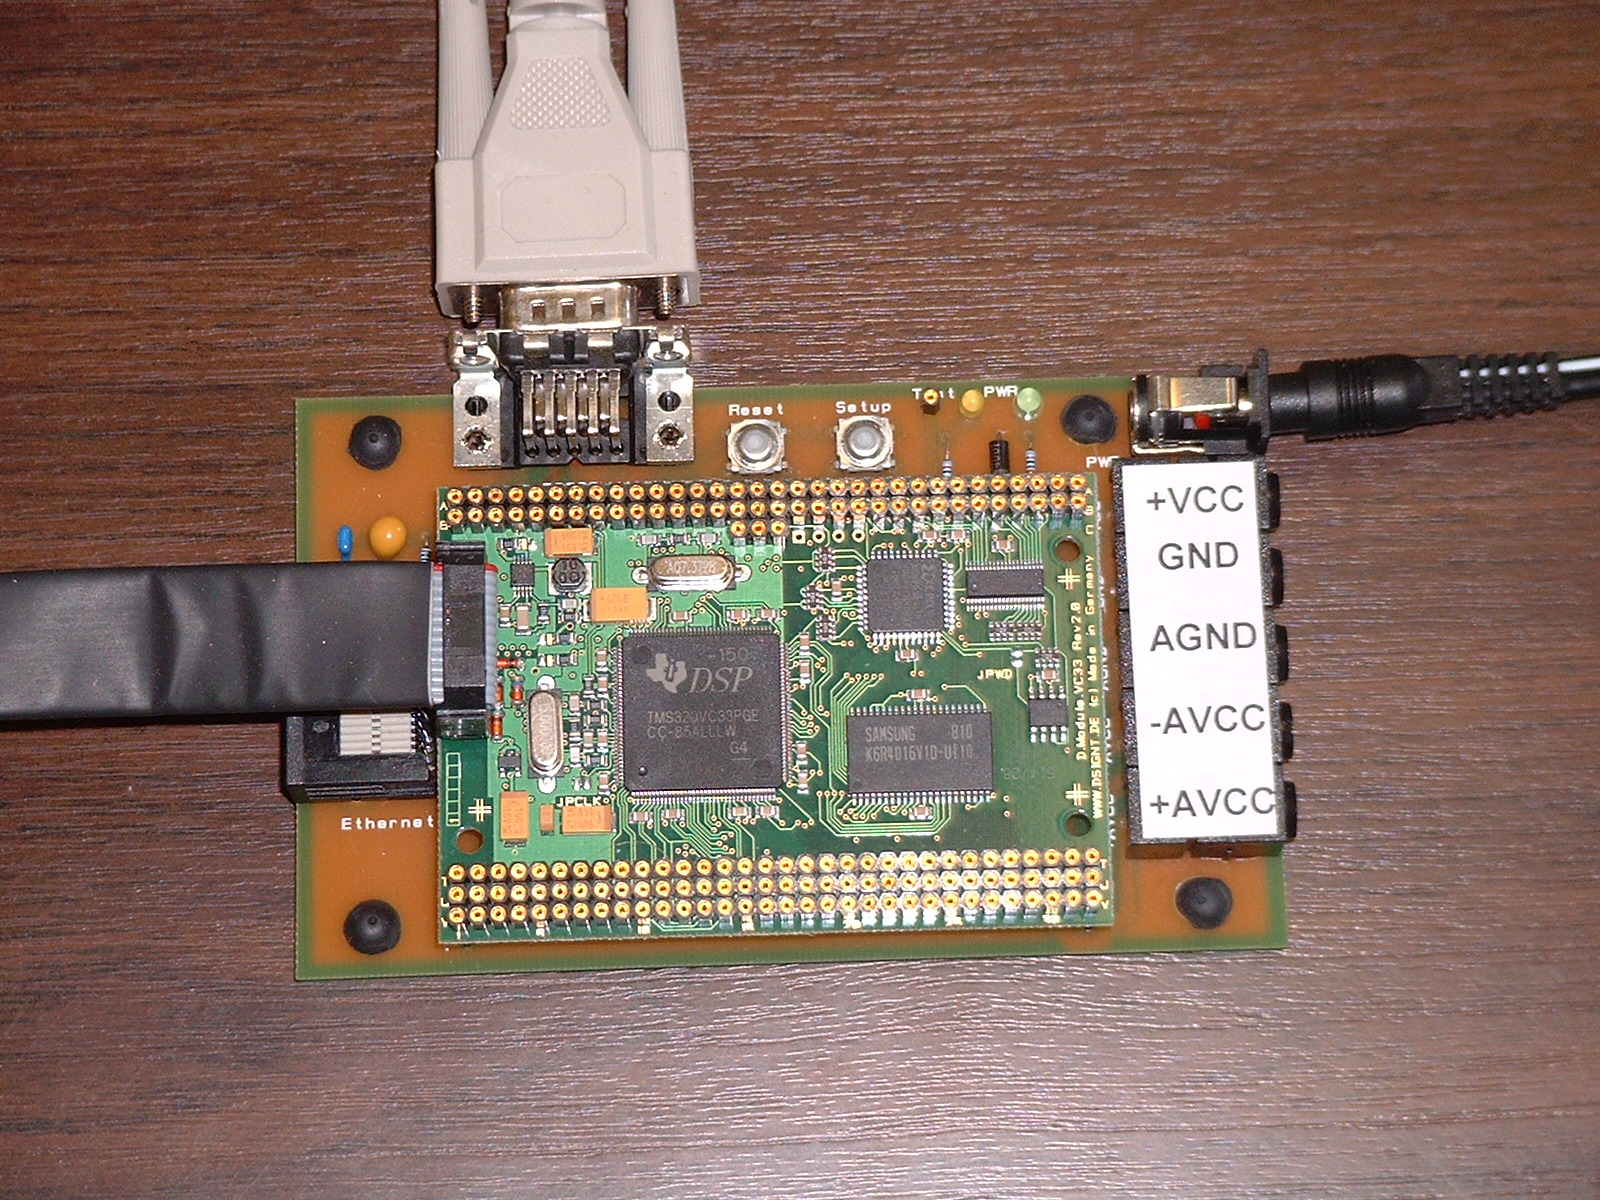
\includegraphics[width=7.0cm]{tms320c3x/fig_tms320c3x_board.jpg}
					\caption{\label{fig:tms320c3x_board} TMS320VC33 Board.}
				\end{center}
			\end{minipage}
			\begin{minipage}{8.0cm}
				\begin{center}
					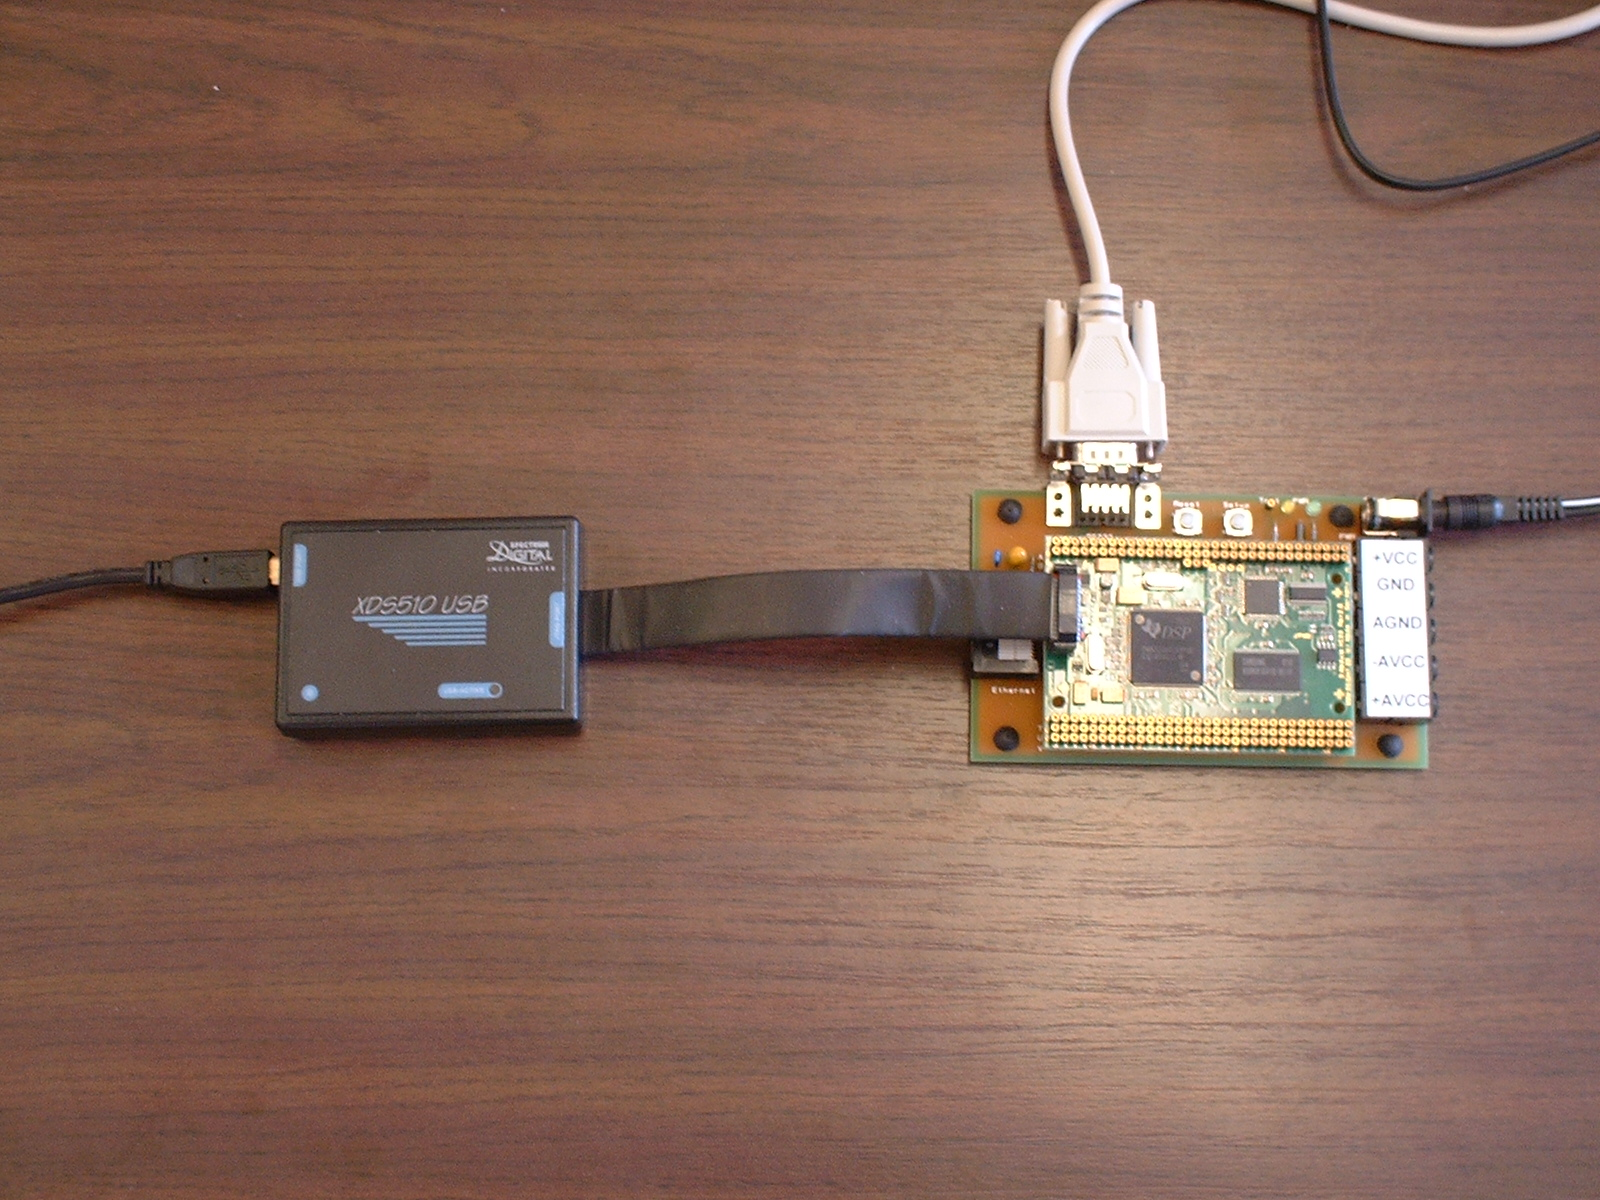
\includegraphics[width=7.0cm]{tms320c3x/fig_tms320c3x_dev_kit.jpg}
					\caption{\label{fig:tms320c3x_jtag_emu} TMS320VC33 board with JTAG.}
				\end{center}
			\end{minipage}
		\end{minipage}
	\end{center}
\end{figure}

The simulator validation involved using the TI C cross-compiler for Windows (see Section~\ref{tms320c3x_cross_compiler}) with the following versions:
\begin{itemize}
\item TMS320C3x/4x ANSI C Compiler Version 5.11
\item TMS320C3x/4x ANSI C Optimizer Version 5.13
\item TMS320C3x/4x ANSI C Code Generator Version 5.13
\item TMS320C3x/4x COFF Assembler Version 5.12
\item TMS320C3x/4x COFF Linker Version 5.11
\end{itemize}

The cross-compiler has generated COFF v2 files for TMS320C3X/C4X with little-endian headers matching the endianness of our building host machine (Windows XP x86).

\noindent The host machine configurations used to test both compilation and run of the simulator are:
\begin{itemize}
\item Redhat Linux RHEL4 x86/gcc 3.4.6 (32-bit little-endian machine)
\item Mandriva Linux 2009.1 x86/gcc 4.3.2 (32-bit little-endian machine)
\item Mandriva Linux 2010.0 x86/gcc 4.4.1 (32-bit little-endian machine)
\item Mageia Linux 3/gcc 4.7.2 (32-bit little-endian machine)
\item Ubuntu Linux 7.04 powerpc/gcc 4.1.2 (32-bit big-endian machine)
\item Ubuntu Linux 9.04 AMD64/x86\_64/gcc 4.3.3 (64-bit little-endian machine)
\item Ubuntu Linux 10.04 AMD64/x86\_64/gcc 4.4.3 (64-bit little-endian machine)
\item Mac OS X Leopard v10.5 x86/gcc 4.3.3 and gcc 4.4.2 (32-bit little-endian machine)
\item Windows XP x86/gcc mingw32 4.4.0 (32 bit little-endian machine)
\end{itemize}

Note that the UNISIM TMS320C3X has also been run under the control of \texttt{valgrind} (\url{http://valgrind.org}), a tool tracking memory related bugs such as memory leaks, unitialized memory reads, and control statements that depends on unitialized variables.

The following developement board (see Figures~\ref{fig:tms320c3x_board}~and~\ref{fig:tms320c3x_jtag_emu}) has been used to compare the simulator results against a real TMS320C3X DSP:
\begin{itemize}
\item A D.SignT DK.VC33-150-S2 development board
\item A D.SignT D.Module.VC33-150-S2 module including a TI TMS320VC33PGE (150 MFLOPS)
\item A 256K 32 bits SRAM with 1 Wait state
\item A 512K 8 bits Flash Memory
\item A Spectrum Digital XDS510USB JTAG Emulator
\item Code Composer IDE 4.10.36 SP2 C3X'C4X for Windows
\end{itemize}

The UNISIM TMS320C3X has been validated using integer benchmarks, floating point benchmarks, and unit tests of individual instructions.
These tests and benchmarks are available for download at \url{http://unisim-vp.org/site/download.html}.
The next sections provide details about the validation process.

\subsection{Benchmarks}
\label{tms320c3x_benchmarks}

This section presents the validation process of UNISIM TMS320C3X simulator using some application benchmarks.
For that purpose, several integer benchmarks have been ported from the MiBench benchmark suite to the TMS320C3X compiler tool chain.
The floating-point benchmarks have been extracted from the TMS320C3x DSK Software.
The following document has been used for selecting these floating-point benchmarks:
\begin{itemize}
\item \textit{TMS320C3x General Purpose Applications User's Guide} (SPRU194, January 1998)
\end{itemize}

These benchmarks have been run into the UNISIM TMS320C3X simulator using the application profiling capability of the inline debugger:
\begin{verbatim}
$ unisim-tms320c3x-2.0 -c sim_config.xml -s enable-inline-debugger=true
Loading xml parameters from: sim_config.xml
Parameters set using file "sim_config.xml"
....

....
loader: Loading symbol table
loader: Loading string table
ti-c-io: TI C I/O support is enabled
ti-c-io: Using __CIOBUF_ at 0xeac00 as I/O buffer
ti-c-io: Installing emulator breakpoint (SWI) for I/O at 0x2003c34 (symbol C$$IO$$)
ti-c-io: Installing emulator breakpoint (SWI) for EXIT at 0x20001cc (symbol C$$EXIT)
Starting simulation at system privilege level
0x00800048 <_c_int00>:
0x00800048:0x08700080 LDP @0x800000
inline-debugger> profile program on
inline-debugger> break C$$EXIT
inline-debugger> continue
...
0x00800073 <C$$EXIT>:
0x00800073:0x66000000 SWI
inline-debugger> profile program
0x00800000 <_enable_insn_cache>:1 times:0x08750800 LDI 2048, ST                                                                                                                                      
0x00800001 <.firm+0x1>:1 times:0x78800000 RETSU <@0x8012a9>                                                                                                                                          
....
0x00801279 <_fclose()+0x39>:3 times:0x0e240000 POP R4
0x0080127a <_fclose()+0x3a>:3 times:0x18740002 SUBI 2, SP
0x0080127b <_fclose()+0x3b>:3 times:0x68000001 BU R1 <_exit()+0x12>
inline-debugger> quit
\end{verbatim}

We extracted the instruction coverage from these applications profiles.
The table below shows the instruction coverage for each benchmark.
Benchmarks \texttt{Fibo}, \texttt{Quick sort}, \texttt{CRC32}, \texttt{Rijndael}, \texttt{Sha}, and \texttt{ADPCM} are integer benchmarks written in C.
Benchmarks \texttt{LP}, \texttt{BP}, \texttt{IIR}, and \texttt{FFT} are floating-point benchmarks written in C and assembly.
Each general addressing mode (see Table~\ref{table:tms320c3x_general_addressing_modes}) of each TMS320C3X instruction (see Tables~\ref{table:tms320c3x_load_store_instructions}, \ref{table:tms320c3x_interlocked_instructions},  \ref{table:tms320c3x_control_instructions}, \ref{table:tms320c3x_2ops_instructions}, \ref{table:tms320c3x_3ops_instructions}, \ref{table:tms320c3x_parallel_instructions} and \ref{table:tms320c3x_power_instructions}), actually has a row in the table.
A tick into a cell at the intersection of a row and a column indicates that the instruction of that row is covered by the benchmark of that column.

Although the integer benchmarks (written in C) have been selected to address the digital signal processing application domain, they have only validated the general operations of the simulator: program loading, program debugging, basic integer computation, control flow instructions, basic addressing modes \ldots
The reason of that limited validation scope is that the C compiler does not generate many different instructions and addressing modes among the integer benchmarks.
For instance, unusual addressing modes as the indirect addressing with circular modify and indirect addressing with bit reversed modify were not generated at all by the C compiler. 
Thus solely relying on these integer benchmarks for testing integer computation would have resulted in quite poor instruction coverage.
For instance, Instructions \texttt{addc}, \texttt{negb}, \texttt{rol}, \texttt{rolc}, \texttt{ror}, \texttt{rorc}, \texttt{subrb}, \texttt{addc3}, \texttt{subb3}, and most of parallel instructions but \texttt{ldi || ldi}, \texttt{ldi || sti}, and \texttt{sti || sti} were not covered at all.
Although the case of floating point benchmarks (written in C and assembly) is similar with an incomplete instruction coverage, the use of assembly has improved coverage of addressing modes and parallel instructions.
For instance, benchmarks \texttt{IIR} and \texttt{FFT} cover indirect addressing with circular modify and indirect addressing with bit reversed modify.
Nevertheless floating-point benchmarks insufficiently cover parallel instructions.
Particularly, Instructions \texttt{absf || stf}, \texttt{fix || sti}, \texttt{float || sti}, \texttt{negf || stf} were not covered at all.

\begin{center}
\tablehead{\hline
\multicolumn{1}{|c|}{\textbf{Instruction}} & \VROT{Fibonacci} & \VROT{Quick sort} & \VROT{CRC32} & \VROT{Rijndael} & \VROT{Sha} & \VROT{ADPCM coder} & \VROT{ADPCM decoder} & \VROT{DCT/Quantization} & \VROT{LP} & \VROT{BP} & \VROT{IIR} & \VROT{FFT}\\
\hline}
\tabletail{\hline}
\begin{supertabular}{|p{7.0cm}|p{0.35cm}|p{0.35cm}|p{0.35cm}|p{0.35cm}|p{0.35cm}|p{0.35cm}|p{0.35cm}|p{0.35cm}|p{0.35cm}|p{0.35cm}|p{0.35cm}|p{0.35cm}|}
\multicolumn{13}{|c|}{\textbf{lde}}\\
\hline
\multicolumn{1}{|p{7.0cm}|}{\scriptsize \texttt{lde reg, reg}} & \multicolumn{1}{p{0.35cm}|}{} & \multicolumn{1}{p{0.35cm}|}{} & \multicolumn{1}{p{0.35cm}|}{} & \multicolumn{1}{p{0.35cm}|}{} & \multicolumn{1}{p{0.35cm}|}{} & \multicolumn{1}{p{0.35cm}|}{} & \multicolumn{1}{p{0.35cm}|}{} & \multicolumn{1}{p{0.35cm}|}{} & \multicolumn{1}{p{0.35cm}|}{} & \multicolumn{1}{p{0.35cm}|}{} & \multicolumn{1}{p{0.35cm}|}{} & \multicolumn{1}{p{0.35cm}|}{\X}\\
\hline
\multicolumn{1}{|p{7.0cm}|}{\scriptsize \texttt{lde dir, reg}} & \multicolumn{1}{p{0.35cm}|}{} & \multicolumn{1}{p{0.35cm}|}{} & \multicolumn{1}{p{0.35cm}|}{} & \multicolumn{1}{p{0.35cm}|}{} & \multicolumn{1}{p{0.35cm}|}{} & \multicolumn{1}{p{0.35cm}|}{} & \multicolumn{1}{p{0.35cm}|}{} & \multicolumn{1}{p{0.35cm}|}{} & \multicolumn{1}{p{0.35cm}|}{} & \multicolumn{1}{p{0.35cm}|}{} & \multicolumn{1}{p{0.35cm}|}{} & \multicolumn{1}{p{0.35cm}|}{}\\
\hline
\multicolumn{1}{|p{7.0cm}|}{\scriptsize \texttt{lde indir, reg}} & \multicolumn{1}{p{0.35cm}|}{} & \multicolumn{1}{p{0.35cm}|}{} & \multicolumn{1}{p{0.35cm}|}{} & \multicolumn{1}{p{0.35cm}|}{} & \multicolumn{1}{p{0.35cm}|}{} & \multicolumn{1}{p{0.35cm}|}{} & \multicolumn{1}{p{0.35cm}|}{} & \multicolumn{1}{p{0.35cm}|}{} & \multicolumn{1}{p{0.35cm}|}{} & \multicolumn{1}{p{0.35cm}|}{} & \multicolumn{1}{p{0.35cm}|}{} & \multicolumn{1}{p{0.35cm}|}{}\\
\hline
\multicolumn{1}{|p{7.0cm}|}{\scriptsize \texttt{lde imm, reg}} & \multicolumn{1}{p{0.35cm}|}{} & \multicolumn{1}{p{0.35cm}|}{} & \multicolumn{1}{p{0.35cm}|}{} & \multicolumn{1}{p{0.35cm}|}{} & \multicolumn{1}{p{0.35cm}|}{} & \multicolumn{1}{p{0.35cm}|}{} & \multicolumn{1}{p{0.35cm}|}{} & \multicolumn{1}{p{0.35cm}|}{} & \multicolumn{1}{p{0.35cm}|}{} & \multicolumn{1}{p{0.35cm}|}{} & \multicolumn{1}{p{0.35cm}|}{} & \multicolumn{1}{p{0.35cm}|}{\X}\\
\hline
\multicolumn{13}{|c|}{\textbf{ldf}}\\
\hline
\multicolumn{1}{|p{7.0cm}|}{\scriptsize \texttt{ldf reg, reg}} & \multicolumn{1}{p{0.35cm}|}{} & \multicolumn{1}{p{0.35cm}|}{} & \multicolumn{1}{p{0.35cm}|}{} & \multicolumn{1}{p{0.35cm}|}{} & \multicolumn{1}{p{0.35cm}|}{} & \multicolumn{1}{p{0.35cm}|}{} & \multicolumn{1}{p{0.35cm}|}{} & \multicolumn{1}{p{0.35cm}|}{} & \multicolumn{1}{p{0.35cm}|}{} & \multicolumn{1}{p{0.35cm}|}{} & \multicolumn{1}{p{0.35cm}|}{\X} & \multicolumn{1}{p{0.35cm}|}{\X}\\
\hline
\multicolumn{1}{|p{7.0cm}|}{\scriptsize \texttt{ldf dir, reg}} & \multicolumn{1}{p{0.35cm}|}{} & \multicolumn{1}{p{0.35cm}|}{} & \multicolumn{1}{p{0.35cm}|}{} & \multicolumn{1}{p{0.35cm}|}{} & \multicolumn{1}{p{0.35cm}|}{} & \multicolumn{1}{p{0.35cm}|}{} & \multicolumn{1}{p{0.35cm}|}{} & \multicolumn{1}{p{0.35cm}|}{} & \multicolumn{1}{p{0.35cm}|}{} & \multicolumn{1}{p{0.35cm}|}{} & \multicolumn{1}{p{0.35cm}|}{} & \multicolumn{1}{p{0.35cm}|}{}\\
\hline
\multicolumn{1}{|p{7.0cm}|}{\scriptsize \texttt{ldf indir, reg}} & \multicolumn{1}{p{0.35cm}|}{} & \multicolumn{1}{p{0.35cm}|}{} & \multicolumn{1}{p{0.35cm}|}{} & \multicolumn{1}{p{0.35cm}|}{} & \multicolumn{1}{p{0.35cm}|}{} & \multicolumn{1}{p{0.35cm}|}{} & \multicolumn{1}{p{0.35cm}|}{} & \multicolumn{1}{p{0.35cm}|}{} & \multicolumn{1}{p{0.35cm}|}{\X} & \multicolumn{1}{p{0.35cm}|}{\X} & \multicolumn{1}{p{0.35cm}|}{\X} & \multicolumn{1}{p{0.35cm}|}{\X}\\
\hline
\multicolumn{1}{|p{7.0cm}|}{\scriptsize \texttt{ldf imm, reg}} & \multicolumn{1}{p{0.35cm}|}{} & \multicolumn{1}{p{0.35cm}|}{} & \multicolumn{1}{p{0.35cm}|}{} & \multicolumn{1}{p{0.35cm}|}{} & \multicolumn{1}{p{0.35cm}|}{} & \multicolumn{1}{p{0.35cm}|}{} & \multicolumn{1}{p{0.35cm}|}{} & \multicolumn{1}{p{0.35cm}|}{} & \multicolumn{1}{p{0.35cm}|}{\X} & \multicolumn{1}{p{0.35cm}|}{\X} & \multicolumn{1}{p{0.35cm}|}{} & \multicolumn{1}{p{0.35cm}|}{\X}\\
\hline
\multicolumn{13}{|c|}{\textbf{ldf\textit{cond}}}\\
\hline
\multicolumn{1}{|p{7.0cm}|}{\scriptsize \texttt{ldf\textit{cond} reg, reg}} & \multicolumn{1}{p{0.35cm}|}{} & \multicolumn{1}{p{0.35cm}|}{} & \multicolumn{1}{p{0.35cm}|}{} & \multicolumn{1}{p{0.35cm}|}{} & \multicolumn{1}{p{0.35cm}|}{} & \multicolumn{1}{p{0.35cm}|}{} & \multicolumn{1}{p{0.35cm}|}{} & \multicolumn{1}{p{0.35cm}|}{} & \multicolumn{1}{p{0.35cm}|}{\X} & \multicolumn{1}{p{0.35cm}|}{\X} & \multicolumn{1}{p{0.35cm}|}{\X} & \multicolumn{1}{p{0.35cm}|}{\X}\\
\hline
\multicolumn{1}{|p{7.0cm}|}{\scriptsize \texttt{ldf\textit{cond} dir, reg}} & \multicolumn{1}{p{0.35cm}|}{} & \multicolumn{1}{p{0.35cm}|}{} & \multicolumn{1}{p{0.35cm}|}{} & \multicolumn{1}{p{0.35cm}|}{} & \multicolumn{1}{p{0.35cm}|}{} & \multicolumn{1}{p{0.35cm}|}{} & \multicolumn{1}{p{0.35cm}|}{} & \multicolumn{1}{p{0.35cm}|}{} & \multicolumn{1}{p{0.35cm}|}{\X} & \multicolumn{1}{p{0.35cm}|}{\X} & \multicolumn{1}{p{0.35cm}|}{\X} & \multicolumn{1}{p{0.35cm}|}{\X}\\
\hline
\multicolumn{1}{|p{7.0cm}|}{\scriptsize \texttt{ldf\textit{cond} indir, reg}} & \multicolumn{1}{p{0.35cm}|}{} & \multicolumn{1}{p{0.35cm}|}{} & \multicolumn{1}{p{0.35cm}|}{} & \multicolumn{1}{p{0.35cm}|}{} & \multicolumn{1}{p{0.35cm}|}{} & \multicolumn{1}{p{0.35cm}|}{} & \multicolumn{1}{p{0.35cm}|}{} & \multicolumn{1}{p{0.35cm}|}{} & \multicolumn{1}{p{0.35cm}|}{} & \multicolumn{1}{p{0.35cm}|}{\X} & \multicolumn{1}{p{0.35cm}|}{\X} & \multicolumn{1}{p{0.35cm}|}{\X}\\
\hline
\multicolumn{1}{|p{7.0cm}|}{\scriptsize \texttt{ldf\textit{cond} imm, reg}} & \multicolumn{1}{p{0.35cm}|}{} & \multicolumn{1}{p{0.35cm}|}{} & \multicolumn{1}{p{0.35cm}|}{} & \multicolumn{1}{p{0.35cm}|}{} & \multicolumn{1}{p{0.35cm}|}{} & \multicolumn{1}{p{0.35cm}|}{} & \multicolumn{1}{p{0.35cm}|}{} & \multicolumn{1}{p{0.35cm}|}{} & \multicolumn{1}{p{0.35cm}|}{\X} & \multicolumn{1}{p{0.35cm}|}{\X} & \multicolumn{1}{p{0.35cm}|}{\X} & \multicolumn{1}{p{0.35cm}|}{\X}\\
\hline
\multicolumn{13}{|c|}{\textbf{ldi}}\\
\hline
\multicolumn{1}{|p{7.0cm}|}{\scriptsize \texttt{ldi reg, reg}} & \multicolumn{1}{p{0.35cm}|}{\X} & \multicolumn{1}{p{0.35cm}|}{\X} & \multicolumn{1}{p{0.35cm}|}{\X} & \multicolumn{1}{p{0.35cm}|}{\X} & \multicolumn{1}{p{0.35cm}|}{\X} & \multicolumn{1}{p{0.35cm}|}{\X} & \multicolumn{1}{p{0.35cm}|}{\X} & \multicolumn{1}{p{0.35cm}|}{\X} & \multicolumn{1}{p{0.35cm}|}{\X} & \multicolumn{1}{p{0.35cm}|}{} & \multicolumn{1}{p{0.35cm}|}{\X} & \multicolumn{1}{p{0.35cm}|}{\X}\\
\hline
\multicolumn{1}{|p{7.0cm}|}{\scriptsize \texttt{ldi dir, reg}} & \multicolumn{1}{p{0.35cm}|}{\X} & \multicolumn{1}{p{0.35cm}|}{\X} & \multicolumn{1}{p{0.35cm}|}{\X} & \multicolumn{1}{p{0.35cm}|}{\X} & \multicolumn{1}{p{0.35cm}|}{\X} & \multicolumn{1}{p{0.35cm}|}{\X} & \multicolumn{1}{p{0.35cm}|}{\X} & \multicolumn{1}{p{0.35cm}|}{\X} & \multicolumn{1}{p{0.35cm}|}{\X} & \multicolumn{1}{p{0.35cm}|}{\X} & \multicolumn{1}{p{0.35cm}|}{\X} & \multicolumn{1}{p{0.35cm}|}{\X}\\
\hline
\multicolumn{1}{|p{7.0cm}|}{\scriptsize \texttt{ldi indir, reg}} & \multicolumn{1}{p{0.35cm}|}{} & \multicolumn{1}{p{0.35cm}|}{\X} & \multicolumn{1}{p{0.35cm}|}{\X} & \multicolumn{1}{p{0.35cm}|}{\X} & \multicolumn{1}{p{0.35cm}|}{\X} & \multicolumn{1}{p{0.35cm}|}{\X} & \multicolumn{1}{p{0.35cm}|}{\X} & \multicolumn{1}{p{0.35cm}|}{} & \multicolumn{1}{p{0.35cm}|}{\X} & \multicolumn{1}{p{0.35cm}|}{\X} & \multicolumn{1}{p{0.35cm}|}{\X} & \multicolumn{1}{p{0.35cm}|}{\X}\\
\hline
\multicolumn{1}{|p{7.0cm}|}{\scriptsize \texttt{ldi imm, reg}} & \multicolumn{1}{p{0.35cm}|}{\X} & \multicolumn{1}{p{0.35cm}|}{\X} & \multicolumn{1}{p{0.35cm}|}{\X} & \multicolumn{1}{p{0.35cm}|}{\X} & \multicolumn{1}{p{0.35cm}|}{\X} & \multicolumn{1}{p{0.35cm}|}{\X} & \multicolumn{1}{p{0.35cm}|}{\X} & \multicolumn{1}{p{0.35cm}|}{\X} & \multicolumn{1}{p{0.35cm}|}{\X} & \multicolumn{1}{p{0.35cm}|}{} & \multicolumn{1}{p{0.35cm}|}{\X} & \multicolumn{1}{p{0.35cm}|}{\X}\\
\hline
\multicolumn{13}{|c|}{\textbf{ldi\textit{cond}}}\\
\hline
\multicolumn{1}{|p{7.0cm}|}{\scriptsize \texttt{ldi\textit{cond} reg, reg}} & \multicolumn{1}{p{0.35cm}|}{\X} & \multicolumn{1}{p{0.35cm}|}{\X} & \multicolumn{1}{p{0.35cm}|}{\X} & \multicolumn{1}{p{0.35cm}|}{\X} & \multicolumn{1}{p{0.35cm}|}{\X} & \multicolumn{1}{p{0.35cm}|}{\X} & \multicolumn{1}{p{0.35cm}|}{\X} & \multicolumn{1}{p{0.35cm}|}{\X} & \multicolumn{1}{p{0.35cm}|}{\X} & \multicolumn{1}{p{0.35cm}|}{\X} & \multicolumn{1}{p{0.35cm}|}{\X} & \multicolumn{1}{p{0.35cm}|}{\X}\\
\hline
\multicolumn{1}{|p{7.0cm}|}{\scriptsize \texttt{ldi\textit{cond} dir, reg}} & \multicolumn{1}{p{0.35cm}|}{\X} & \multicolumn{1}{p{0.35cm}|}{\X} & \multicolumn{1}{p{0.35cm}|}{\X} & \multicolumn{1}{p{0.35cm}|}{\X} & \multicolumn{1}{p{0.35cm}|}{\X} & \multicolumn{1}{p{0.35cm}|}{\X} & \multicolumn{1}{p{0.35cm}|}{\X} & \multicolumn{1}{p{0.35cm}|}{\X} & \multicolumn{1}{p{0.35cm}|}{\X} & \multicolumn{1}{p{0.35cm}|}{\X} & \multicolumn{1}{p{0.35cm}|}{\X} & \multicolumn{1}{p{0.35cm}|}{\X}\\
\hline
\multicolumn{1}{|p{7.0cm}|}{\scriptsize \texttt{ldi\textit{cond} indir, reg}} & \multicolumn{1}{p{0.35cm}|}{\X} & \multicolumn{1}{p{0.35cm}|}{\X} & \multicolumn{1}{p{0.35cm}|}{\X} & \multicolumn{1}{p{0.35cm}|}{\X} & \multicolumn{1}{p{0.35cm}|}{\X} & \multicolumn{1}{p{0.35cm}|}{\X} & \multicolumn{1}{p{0.35cm}|}{\X} & \multicolumn{1}{p{0.35cm}|}{\X} & \multicolumn{1}{p{0.35cm}|}{\X} & \multicolumn{1}{p{0.35cm}|}{\X} & \multicolumn{1}{p{0.35cm}|}{\X} & \multicolumn{1}{p{0.35cm}|}{\X}\\
\hline
\multicolumn{1}{|p{7.0cm}|}{\scriptsize \texttt{ldi\textit{cond} imm, reg}} & \multicolumn{1}{p{0.35cm}|}{\X} & \multicolumn{1}{p{0.35cm}|}{\X} & \multicolumn{1}{p{0.35cm}|}{\X} & \multicolumn{1}{p{0.35cm}|}{\X} & \multicolumn{1}{p{0.35cm}|}{\X} & \multicolumn{1}{p{0.35cm}|}{\X} & \multicolumn{1}{p{0.35cm}|}{\X} & \multicolumn{1}{p{0.35cm}|}{\X} & \multicolumn{1}{p{0.35cm}|}{\X} & \multicolumn{1}{p{0.35cm}|}{\X} & \multicolumn{1}{p{0.35cm}|}{\X} & \multicolumn{1}{p{0.35cm}|}{\X}\\
\hline
\multicolumn{13}{|c|}{\textbf{ldm}}\\
\hline
\multicolumn{1}{|p{7.0cm}|}{\scriptsize \texttt{ldm reg, reg}} & \multicolumn{1}{p{0.35cm}|}{} & \multicolumn{1}{p{0.35cm}|}{} & \multicolumn{1}{p{0.35cm}|}{} & \multicolumn{1}{p{0.35cm}|}{} & \multicolumn{1}{p{0.35cm}|}{} & \multicolumn{1}{p{0.35cm}|}{} & \multicolumn{1}{p{0.35cm}|}{} & \multicolumn{1}{p{0.35cm}|}{} & \multicolumn{1}{p{0.35cm}|}{} & \multicolumn{1}{p{0.35cm}|}{} & \multicolumn{1}{p{0.35cm}|}{} & \multicolumn{1}{p{0.35cm}|}{}\\
\hline
\multicolumn{1}{|p{7.0cm}|}{\scriptsize \texttt{ldm dir, reg}} & \multicolumn{1}{p{0.35cm}|}{} & \multicolumn{1}{p{0.35cm}|}{} & \multicolumn{1}{p{0.35cm}|}{} & \multicolumn{1}{p{0.35cm}|}{} & \multicolumn{1}{p{0.35cm}|}{} & \multicolumn{1}{p{0.35cm}|}{} & \multicolumn{1}{p{0.35cm}|}{} & \multicolumn{1}{p{0.35cm}|}{} & \multicolumn{1}{p{0.35cm}|}{} & \multicolumn{1}{p{0.35cm}|}{} & \multicolumn{1}{p{0.35cm}|}{} & \multicolumn{1}{p{0.35cm}|}{}\\
\hline
\multicolumn{1}{|p{7.0cm}|}{\scriptsize \texttt{ldm indir, reg}} & \multicolumn{1}{p{0.35cm}|}{} & \multicolumn{1}{p{0.35cm}|}{} & \multicolumn{1}{p{0.35cm}|}{} & \multicolumn{1}{p{0.35cm}|}{} & \multicolumn{1}{p{0.35cm}|}{} & \multicolumn{1}{p{0.35cm}|}{} & \multicolumn{1}{p{0.35cm}|}{} & \multicolumn{1}{p{0.35cm}|}{} & \multicolumn{1}{p{0.35cm}|}{} & \multicolumn{1}{p{0.35cm}|}{} & \multicolumn{1}{p{0.35cm}|}{} & \multicolumn{1}{p{0.35cm}|}{}\\
\hline
\multicolumn{1}{|p{7.0cm}|}{\scriptsize \texttt{ldm imm, reg}} & \multicolumn{1}{p{0.35cm}|}{} & \multicolumn{1}{p{0.35cm}|}{} & \multicolumn{1}{p{0.35cm}|}{} & \multicolumn{1}{p{0.35cm}|}{} & \multicolumn{1}{p{0.35cm}|}{} & \multicolumn{1}{p{0.35cm}|}{} & \multicolumn{1}{p{0.35cm}|}{} & \multicolumn{1}{p{0.35cm}|}{} & \multicolumn{1}{p{0.35cm}|}{} & \multicolumn{1}{p{0.35cm}|}{} & \multicolumn{1}{p{0.35cm}|}{} & \multicolumn{1}{p{0.35cm}|}{\X}\\
\hline
\multicolumn{13}{|c|}{\textbf{ldp}}\\
\hline
\multicolumn{1}{|p{7.0cm}|}{\scriptsize \texttt{ldp src}} & \multicolumn{1}{p{0.35cm}|}{\X} & \multicolumn{1}{p{0.35cm}|}{\X} & \multicolumn{1}{p{0.35cm}|}{\X} & \multicolumn{1}{p{0.35cm}|}{\X} & \multicolumn{1}{p{0.35cm}|}{\X} & \multicolumn{1}{p{0.35cm}|}{\X} & \multicolumn{1}{p{0.35cm}|}{\X} & \multicolumn{1}{p{0.35cm}|}{\X} & \multicolumn{1}{p{0.35cm}|}{\X} & \multicolumn{1}{p{0.35cm}|}{\X} & \multicolumn{1}{p{0.35cm}|}{\X} & \multicolumn{1}{p{0.35cm}|}{\X}\\
\hline
\multicolumn{13}{|c|}{\textbf{pop}}\\
\hline
\multicolumn{1}{|p{7.0cm}|}{\scriptsize \texttt{pop reg}} & \multicolumn{1}{p{0.35cm}|}{\X} & \multicolumn{1}{p{0.35cm}|}{\X} & \multicolumn{1}{p{0.35cm}|}{\X} & \multicolumn{1}{p{0.35cm}|}{\X} & \multicolumn{1}{p{0.35cm}|}{\X} & \multicolumn{1}{p{0.35cm}|}{\X} & \multicolumn{1}{p{0.35cm}|}{\X} & \multicolumn{1}{p{0.35cm}|}{\X} & \multicolumn{1}{p{0.35cm}|}{\X} & \multicolumn{1}{p{0.35cm}|}{\X} & \multicolumn{1}{p{0.35cm}|}{\X} & \multicolumn{1}{p{0.35cm}|}{\X}\\
\hline
\multicolumn{13}{|c|}{\textbf{popf}}\\
\hline
\multicolumn{1}{|p{7.0cm}|}{\scriptsize \texttt{popf reg}} & \multicolumn{1}{p{0.35cm}|}{} & \multicolumn{1}{p{0.35cm}|}{} & \multicolumn{1}{p{0.35cm}|}{} & \multicolumn{1}{p{0.35cm}|}{\X} & \multicolumn{1}{p{0.35cm}|}{\X} & \multicolumn{1}{p{0.35cm}|}{\X} & \multicolumn{1}{p{0.35cm}|}{\X} & \multicolumn{1}{p{0.35cm}|}{\X} & \multicolumn{1}{p{0.35cm}|}{\X} & \multicolumn{1}{p{0.35cm}|}{\X} & \multicolumn{1}{p{0.35cm}|}{\X} & \multicolumn{1}{p{0.35cm}|}{\X}\\
\hline
\multicolumn{13}{|c|}{\textbf{push}}\\
\hline
\multicolumn{1}{|p{7.0cm}|}{\scriptsize \texttt{push reg}} & \multicolumn{1}{p{0.35cm}|}{\X} & \multicolumn{1}{p{0.35cm}|}{\X} & \multicolumn{1}{p{0.35cm}|}{\X} & \multicolumn{1}{p{0.35cm}|}{\X} & \multicolumn{1}{p{0.35cm}|}{\X} & \multicolumn{1}{p{0.35cm}|}{\X} & \multicolumn{1}{p{0.35cm}|}{\X} & \multicolumn{1}{p{0.35cm}|}{\X} & \multicolumn{1}{p{0.35cm}|}{\X} & \multicolumn{1}{p{0.35cm}|}{\X} & \multicolumn{1}{p{0.35cm}|}{\X} & \multicolumn{1}{p{0.35cm}|}{\X}\\
\hline
\multicolumn{13}{|c|}{\textbf{pushf}}\\
\hline
\multicolumn{1}{|p{7.0cm}|}{\scriptsize \texttt{pushf reg}} & \multicolumn{1}{p{0.35cm}|}{\X} & \multicolumn{1}{p{0.35cm}|}{\X} & \multicolumn{1}{p{0.35cm}|}{\X} & \multicolumn{1}{p{0.35cm}|}{\X} & \multicolumn{1}{p{0.35cm}|}{\X} & \multicolumn{1}{p{0.35cm}|}{\X} & \multicolumn{1}{p{0.35cm}|}{\X} & \multicolumn{1}{p{0.35cm}|}{\X} & \multicolumn{1}{p{0.35cm}|}{\X} & \multicolumn{1}{p{0.35cm}|}{\X} & \multicolumn{1}{p{0.35cm}|}{\X} & \multicolumn{1}{p{0.35cm}|}{\X}\\
\hline
\multicolumn{13}{|c|}{\textbf{stf}}\\
\hline
\multicolumn{1}{|p{7.0cm}|}{\scriptsize \texttt{stf reg, dir}} & \multicolumn{1}{p{0.35cm}|}{} & \multicolumn{1}{p{0.35cm}|}{} & \multicolumn{1}{p{0.35cm}|}{} & \multicolumn{1}{p{0.35cm}|}{} & \multicolumn{1}{p{0.35cm}|}{} & \multicolumn{1}{p{0.35cm}|}{} & \multicolumn{1}{p{0.35cm}|}{} & \multicolumn{1}{p{0.35cm}|}{} & \multicolumn{1}{p{0.35cm}|}{} & \multicolumn{1}{p{0.35cm}|}{} & \multicolumn{1}{p{0.35cm}|}{\X} & \multicolumn{1}{p{0.35cm}|}{}\\
\hline
\multicolumn{1}{|p{7.0cm}|}{\scriptsize \texttt{stf reg, indir}} & \multicolumn{1}{p{0.35cm}|}{} & \multicolumn{1}{p{0.35cm}|}{} & \multicolumn{1}{p{0.35cm}|}{} & \multicolumn{1}{p{0.35cm}|}{} & \multicolumn{1}{p{0.35cm}|}{} & \multicolumn{1}{p{0.35cm}|}{} & \multicolumn{1}{p{0.35cm}|}{} & \multicolumn{1}{p{0.35cm}|}{} & \multicolumn{1}{p{0.35cm}|}{\X} & \multicolumn{1}{p{0.35cm}|}{\X} & \multicolumn{1}{p{0.35cm}|}{\X} & \multicolumn{1}{p{0.35cm}|}{\X}\\
\hline
\multicolumn{13}{|c|}{\textbf{sti}}\\
\hline
\multicolumn{1}{|p{7.0cm}|}{\scriptsize \texttt{sti reg, dir}} & \multicolumn{1}{p{0.35cm}|}{\X} & \multicolumn{1}{p{0.35cm}|}{\X} & \multicolumn{1}{p{0.35cm}|}{\X} & \multicolumn{1}{p{0.35cm}|}{\X} & \multicolumn{1}{p{0.35cm}|}{\X} & \multicolumn{1}{p{0.35cm}|}{\X} & \multicolumn{1}{p{0.35cm}|}{\X} & \multicolumn{1}{p{0.35cm}|}{\X} & \multicolumn{1}{p{0.35cm}|}{\X} & \multicolumn{1}{p{0.35cm}|}{\X} & \multicolumn{1}{p{0.35cm}|}{\X} & \multicolumn{1}{p{0.35cm}|}{\X}\\
\hline
\multicolumn{1}{|p{7.0cm}|}{\scriptsize \texttt{sti reg, indir}} & \multicolumn{1}{p{0.35cm}|}{\X} & \multicolumn{1}{p{0.35cm}|}{\X} & \multicolumn{1}{p{0.35cm}|}{\X} & \multicolumn{1}{p{0.35cm}|}{\X} & \multicolumn{1}{p{0.35cm}|}{\X} & \multicolumn{1}{p{0.35cm}|}{\X} & \multicolumn{1}{p{0.35cm}|}{\X} & \multicolumn{1}{p{0.35cm}|}{\X} & \multicolumn{1}{p{0.35cm}|}{\X} & \multicolumn{1}{p{0.35cm}|}{\X} & \multicolumn{1}{p{0.35cm}|}{\X} & \multicolumn{1}{p{0.35cm}|}{\X}\\
\hline
\multicolumn{13}{|c|}{\textbf{ldfi}}\\
\hline
\multicolumn{1}{|p{7.0cm}|}{\scriptsize \texttt{ldfi dir, reg}} & \multicolumn{1}{p{0.35cm}|}{} & \multicolumn{1}{p{0.35cm}|}{} & \multicolumn{1}{p{0.35cm}|}{} & \multicolumn{1}{p{0.35cm}|}{} & \multicolumn{1}{p{0.35cm}|}{} & \multicolumn{1}{p{0.35cm}|}{} & \multicolumn{1}{p{0.35cm}|}{} & \multicolumn{1}{p{0.35cm}|}{} & \multicolumn{1}{p{0.35cm}|}{} & \multicolumn{1}{p{0.35cm}|}{} & \multicolumn{1}{p{0.35cm}|}{} & \multicolumn{1}{p{0.35cm}|}{}\\
\hline
\multicolumn{1}{|p{7.0cm}|}{\scriptsize \texttt{ldfi indir, reg}} & \multicolumn{1}{p{0.35cm}|}{} & \multicolumn{1}{p{0.35cm}|}{} & \multicolumn{1}{p{0.35cm}|}{} & \multicolumn{1}{p{0.35cm}|}{} & \multicolumn{1}{p{0.35cm}|}{} & \multicolumn{1}{p{0.35cm}|}{} & \multicolumn{1}{p{0.35cm}|}{} & \multicolumn{1}{p{0.35cm}|}{} & \multicolumn{1}{p{0.35cm}|}{} & \multicolumn{1}{p{0.35cm}|}{} & \multicolumn{1}{p{0.35cm}|}{} & \multicolumn{1}{p{0.35cm}|}{}\\
\hline
\multicolumn{13}{|c|}{\textbf{ldii}}\\
\hline
\multicolumn{1}{|p{7.0cm}|}{\scriptsize \texttt{ldii dir, reg}} & \multicolumn{1}{p{0.35cm}|}{} & \multicolumn{1}{p{0.35cm}|}{} & \multicolumn{1}{p{0.35cm}|}{} & \multicolumn{1}{p{0.35cm}|}{} & \multicolumn{1}{p{0.35cm}|}{} & \multicolumn{1}{p{0.35cm}|}{} & \multicolumn{1}{p{0.35cm}|}{} & \multicolumn{1}{p{0.35cm}|}{} & \multicolumn{1}{p{0.35cm}|}{} & \multicolumn{1}{p{0.35cm}|}{} & \multicolumn{1}{p{0.35cm}|}{} & \multicolumn{1}{p{0.35cm}|}{}\\
\hline
\multicolumn{1}{|p{7.0cm}|}{\scriptsize \texttt{ldii indir, reg}} & \multicolumn{1}{p{0.35cm}|}{} & \multicolumn{1}{p{0.35cm}|}{} & \multicolumn{1}{p{0.35cm}|}{} & \multicolumn{1}{p{0.35cm}|}{} & \multicolumn{1}{p{0.35cm}|}{} & \multicolumn{1}{p{0.35cm}|}{} & \multicolumn{1}{p{0.35cm}|}{} & \multicolumn{1}{p{0.35cm}|}{} & \multicolumn{1}{p{0.35cm}|}{} & \multicolumn{1}{p{0.35cm}|}{} & \multicolumn{1}{p{0.35cm}|}{} & \multicolumn{1}{p{0.35cm}|}{}\\
\hline
\multicolumn{13}{|c|}{\textbf{sigi}}\\
\hline
\multicolumn{1}{|p{7.0cm}|}{\scriptsize \texttt{sigi}} & \multicolumn{1}{p{0.35cm}|}{} & \multicolumn{1}{p{0.35cm}|}{} & \multicolumn{1}{p{0.35cm}|}{} & \multicolumn{1}{p{0.35cm}|}{} & \multicolumn{1}{p{0.35cm}|}{} & \multicolumn{1}{p{0.35cm}|}{} & \multicolumn{1}{p{0.35cm}|}{} & \multicolumn{1}{p{0.35cm}|}{} & \multicolumn{1}{p{0.35cm}|}{} & \multicolumn{1}{p{0.35cm}|}{} & \multicolumn{1}{p{0.35cm}|}{} & \multicolumn{1}{p{0.35cm}|}{}\\
\hline
\multicolumn{13}{|c|}{\textbf{stfi}}\\
\hline
\multicolumn{1}{|p{7.0cm}|}{\scriptsize \texttt{stfi reg, dir}} & \multicolumn{1}{p{0.35cm}|}{} & \multicolumn{1}{p{0.35cm}|}{} & \multicolumn{1}{p{0.35cm}|}{} & \multicolumn{1}{p{0.35cm}|}{} & \multicolumn{1}{p{0.35cm}|}{} & \multicolumn{1}{p{0.35cm}|}{} & \multicolumn{1}{p{0.35cm}|}{} & \multicolumn{1}{p{0.35cm}|}{} & \multicolumn{1}{p{0.35cm}|}{} & \multicolumn{1}{p{0.35cm}|}{} & \multicolumn{1}{p{0.35cm}|}{} & \multicolumn{1}{p{0.35cm}|}{}\\
\hline
\multicolumn{1}{|p{7.0cm}|}{\scriptsize \texttt{stfi reg, indir}} & \multicolumn{1}{p{0.35cm}|}{} & \multicolumn{1}{p{0.35cm}|}{} & \multicolumn{1}{p{0.35cm}|}{} & \multicolumn{1}{p{0.35cm}|}{} & \multicolumn{1}{p{0.35cm}|}{} & \multicolumn{1}{p{0.35cm}|}{} & \multicolumn{1}{p{0.35cm}|}{} & \multicolumn{1}{p{0.35cm}|}{} & \multicolumn{1}{p{0.35cm}|}{} & \multicolumn{1}{p{0.35cm}|}{} & \multicolumn{1}{p{0.35cm}|}{} & \multicolumn{1}{p{0.35cm}|}{}\\
\hline
\multicolumn{13}{|c|}{\textbf{stii}}\\
\hline
\multicolumn{1}{|p{7.0cm}|}{\scriptsize \texttt{stii reg, dir}} & \multicolumn{1}{p{0.35cm}|}{} & \multicolumn{1}{p{0.35cm}|}{} & \multicolumn{1}{p{0.35cm}|}{} & \multicolumn{1}{p{0.35cm}|}{} & \multicolumn{1}{p{0.35cm}|}{} & \multicolumn{1}{p{0.35cm}|}{} & \multicolumn{1}{p{0.35cm}|}{} & \multicolumn{1}{p{0.35cm}|}{} & \multicolumn{1}{p{0.35cm}|}{} & \multicolumn{1}{p{0.35cm}|}{} & \multicolumn{1}{p{0.35cm}|}{} & \multicolumn{1}{p{0.35cm}|}{}\\
\hline
\multicolumn{1}{|p{7.0cm}|}{\scriptsize \texttt{stii reg, indir}} & \multicolumn{1}{p{0.35cm}|}{} & \multicolumn{1}{p{0.35cm}|}{} & \multicolumn{1}{p{0.35cm}|}{} & \multicolumn{1}{p{0.35cm}|}{} & \multicolumn{1}{p{0.35cm}|}{} & \multicolumn{1}{p{0.35cm}|}{} & \multicolumn{1}{p{0.35cm}|}{} & \multicolumn{1}{p{0.35cm}|}{} & \multicolumn{1}{p{0.35cm}|}{} & \multicolumn{1}{p{0.35cm}|}{} & \multicolumn{1}{p{0.35cm}|}{} & \multicolumn{1}{p{0.35cm}|}{}\\
\hline
\multicolumn{13}{|c|}{\textbf{b\textit{cond}}}\\
\hline
\multicolumn{1}{|p{7.0cm}|}{\scriptsize \texttt{b\textit{cond} reg}} & \multicolumn{1}{p{0.35cm}|}{\X} & \multicolumn{1}{p{0.35cm}|}{\X} & \multicolumn{1}{p{0.35cm}|}{\X} & \multicolumn{1}{p{0.35cm}|}{\X} & \multicolumn{1}{p{0.35cm}|}{\X} & \multicolumn{1}{p{0.35cm}|}{\X} & \multicolumn{1}{p{0.35cm}|}{\X} & \multicolumn{1}{p{0.35cm}|}{\X} & \multicolumn{1}{p{0.35cm}|}{} & \multicolumn{1}{p{0.35cm}|}{} & \multicolumn{1}{p{0.35cm}|}{} & \multicolumn{1}{p{0.35cm}|}{\X}\\
\hline
\multicolumn{1}{|p{7.0cm}|}{\scriptsize \texttt{b\textit{cond} disp}} & \multicolumn{1}{p{0.35cm}|}{\X} & \multicolumn{1}{p{0.35cm}|}{\X} & \multicolumn{1}{p{0.35cm}|}{\X} & \multicolumn{1}{p{0.35cm}|}{\X} & \multicolumn{1}{p{0.35cm}|}{\X} & \multicolumn{1}{p{0.35cm}|}{\X} & \multicolumn{1}{p{0.35cm}|}{\X} & \multicolumn{1}{p{0.35cm}|}{\X} & \multicolumn{1}{p{0.35cm}|}{\X} & \multicolumn{1}{p{0.35cm}|}{\X} & \multicolumn{1}{p{0.35cm}|}{\X} & \multicolumn{1}{p{0.35cm}|}{\X}\\
\hline
\multicolumn{13}{|c|}{\textbf{b\textit{cond}d}}\\
\hline
\multicolumn{1}{|p{7.0cm}|}{\scriptsize \texttt{b\textit{cond}d reg}} & \multicolumn{1}{p{0.35cm}|}{\X} & \multicolumn{1}{p{0.35cm}|}{\X} & \multicolumn{1}{p{0.35cm}|}{\X} & \multicolumn{1}{p{0.35cm}|}{\X} & \multicolumn{1}{p{0.35cm}|}{\X} & \multicolumn{1}{p{0.35cm}|}{\X} & \multicolumn{1}{p{0.35cm}|}{\X} & \multicolumn{1}{p{0.35cm}|}{\X} & \multicolumn{1}{p{0.35cm}|}{} & \multicolumn{1}{p{0.35cm}|}{} & \multicolumn{1}{p{0.35cm}|}{} & \multicolumn{1}{p{0.35cm}|}{\X}\\
\hline
\multicolumn{1}{|p{7.0cm}|}{\scriptsize \texttt{b\textit{cond}d disp}} & \multicolumn{1}{p{0.35cm}|}{\X} & \multicolumn{1}{p{0.35cm}|}{\X} & \multicolumn{1}{p{0.35cm}|}{\X} & \multicolumn{1}{p{0.35cm}|}{\X} & \multicolumn{1}{p{0.35cm}|}{\X} & \multicolumn{1}{p{0.35cm}|}{\X} & \multicolumn{1}{p{0.35cm}|}{\X} & \multicolumn{1}{p{0.35cm}|}{\X} & \multicolumn{1}{p{0.35cm}|}{\X} & \multicolumn{1}{p{0.35cm}|}{\X} & \multicolumn{1}{p{0.35cm}|}{\X} & \multicolumn{1}{p{0.35cm}|}{\X}\\
\hline
\multicolumn{13}{|c|}{\textbf{br}}\\
\hline
\multicolumn{1}{|p{7.0cm}|}{\scriptsize \texttt{br src}} & \multicolumn{1}{p{0.35cm}|}{} & \multicolumn{1}{p{0.35cm}|}{} & \multicolumn{1}{p{0.35cm}|}{} & \multicolumn{1}{p{0.35cm}|}{} & \multicolumn{1}{p{0.35cm}|}{} & \multicolumn{1}{p{0.35cm}|}{} & \multicolumn{1}{p{0.35cm}|}{} & \multicolumn{1}{p{0.35cm}|}{} & \multicolumn{1}{p{0.35cm}|}{} & \multicolumn{1}{p{0.35cm}|}{} & \multicolumn{1}{p{0.35cm}|}{} & \multicolumn{1}{p{0.35cm}|}{}\\
\hline
\multicolumn{13}{|c|}{\textbf{brd}}\\
\hline
\multicolumn{1}{|p{7.0cm}|}{\scriptsize \texttt{brd src}} & \multicolumn{1}{p{0.35cm}|}{} & \multicolumn{1}{p{0.35cm}|}{} & \multicolumn{1}{p{0.35cm}|}{} & \multicolumn{1}{p{0.35cm}|}{} & \multicolumn{1}{p{0.35cm}|}{} & \multicolumn{1}{p{0.35cm}|}{} & \multicolumn{1}{p{0.35cm}|}{} & \multicolumn{1}{p{0.35cm}|}{} & \multicolumn{1}{p{0.35cm}|}{} & \multicolumn{1}{p{0.35cm}|}{} & \multicolumn{1}{p{0.35cm}|}{} & \multicolumn{1}{p{0.35cm}|}{}\\
\hline
\multicolumn{13}{|c|}{\textbf{call}}\\
\hline
\multicolumn{1}{|p{7.0cm}|}{\scriptsize \texttt{call src}} & \multicolumn{1}{p{0.35cm}|}{\X} & \multicolumn{1}{p{0.35cm}|}{\X} & \multicolumn{1}{p{0.35cm}|}{\X} & \multicolumn{1}{p{0.35cm}|}{\X} & \multicolumn{1}{p{0.35cm}|}{\X} & \multicolumn{1}{p{0.35cm}|}{\X} & \multicolumn{1}{p{0.35cm}|}{\X} & \multicolumn{1}{p{0.35cm}|}{\X} & \multicolumn{1}{p{0.35cm}|}{} & \multicolumn{1}{p{0.35cm}|}{\X} & \multicolumn{1}{p{0.35cm}|}{\X} & \multicolumn{1}{p{0.35cm}|}{\X}\\
\hline
\multicolumn{13}{|c|}{\textbf{call\textit{cond}}}\\
\hline
\multicolumn{1}{|p{7.0cm}|}{\scriptsize \texttt{call\textit{cond} reg}} & \multicolumn{1}{p{0.35cm}|}{\X} & \multicolumn{1}{p{0.35cm}|}{\X} & \multicolumn{1}{p{0.35cm}|}{\X} & \multicolumn{1}{p{0.35cm}|}{\X} & \multicolumn{1}{p{0.35cm}|}{\X} & \multicolumn{1}{p{0.35cm}|}{\X} & \multicolumn{1}{p{0.35cm}|}{\X} & \multicolumn{1}{p{0.35cm}|}{\X} & \multicolumn{1}{p{0.35cm}|}{\X} & \multicolumn{1}{p{0.35cm}|}{\X} & \multicolumn{1}{p{0.35cm}|}{\X} & \multicolumn{1}{p{0.35cm}|}{\X}\\
\hline
\multicolumn{1}{|p{7.0cm}|}{\scriptsize \texttt{call\textit{cond} disp}} & \multicolumn{1}{p{0.35cm}|}{} & \multicolumn{1}{p{0.35cm}|}{} & \multicolumn{1}{p{0.35cm}|}{} & \multicolumn{1}{p{0.35cm}|}{} & \multicolumn{1}{p{0.35cm}|}{} & \multicolumn{1}{p{0.35cm}|}{} & \multicolumn{1}{p{0.35cm}|}{} & \multicolumn{1}{p{0.35cm}|}{} & \multicolumn{1}{p{0.35cm}|}{\X} & \multicolumn{1}{p{0.35cm}|}{} & \multicolumn{1}{p{0.35cm}|}{} & \multicolumn{1}{p{0.35cm}|}{\X}\\
\hline
\multicolumn{13}{|c|}{\textbf{db\textit{cond}}}\\
\hline
\multicolumn{1}{|p{7.0cm}|}{\scriptsize \texttt{db\textit{cond} ar$_n$, reg}} & \multicolumn{1}{p{0.35cm}|}{} & \multicolumn{1}{p{0.35cm}|}{} & \multicolumn{1}{p{0.35cm}|}{} & \multicolumn{1}{p{0.35cm}|}{} & \multicolumn{1}{p{0.35cm}|}{} & \multicolumn{1}{p{0.35cm}|}{} & \multicolumn{1}{p{0.35cm}|}{} & \multicolumn{1}{p{0.35cm}|}{} & \multicolumn{1}{p{0.35cm}|}{} & \multicolumn{1}{p{0.35cm}|}{} & \multicolumn{1}{p{0.35cm}|}{} & \multicolumn{1}{p{0.35cm}|}{}\\
\hline
\multicolumn{1}{|p{7.0cm}|}{\scriptsize \texttt{db\textit{cond} ar$_n$, disp}} & \multicolumn{1}{p{0.35cm}|}{} & \multicolumn{1}{p{0.35cm}|}{} & \multicolumn{1}{p{0.35cm}|}{} & \multicolumn{1}{p{0.35cm}|}{\X} & \multicolumn{1}{p{0.35cm}|}{} & \multicolumn{1}{p{0.35cm}|}{} & \multicolumn{1}{p{0.35cm}|}{} & \multicolumn{1}{p{0.35cm}|}{\X} & \multicolumn{1}{p{0.35cm}|}{} & \multicolumn{1}{p{0.35cm}|}{} & \multicolumn{1}{p{0.35cm}|}{} & \multicolumn{1}{p{0.35cm}|}{\X}\\
\hline
\multicolumn{13}{|c|}{\textbf{db\textit{cond}d}}\\
\hline
\multicolumn{1}{|p{7.0cm}|}{\scriptsize \texttt{db\textit{cond}d ar$_n$, reg}} & \multicolumn{1}{p{0.35cm}|}{} & \multicolumn{1}{p{0.35cm}|}{} & \multicolumn{1}{p{0.35cm}|}{} & \multicolumn{1}{p{0.35cm}|}{} & \multicolumn{1}{p{0.35cm}|}{} & \multicolumn{1}{p{0.35cm}|}{} & \multicolumn{1}{p{0.35cm}|}{} & \multicolumn{1}{p{0.35cm}|}{} & \multicolumn{1}{p{0.35cm}|}{} & \multicolumn{1}{p{0.35cm}|}{} & \multicolumn{1}{p{0.35cm}|}{} & \multicolumn{1}{p{0.35cm}|}{}\\
\hline
\multicolumn{1}{|p{7.0cm}|}{\scriptsize \texttt{db\textit{cond}d ar$_n$, disp}} & \multicolumn{1}{p{0.35cm}|}{} & \multicolumn{1}{p{0.35cm}|}{} & \multicolumn{1}{p{0.35cm}|}{} & \multicolumn{1}{p{0.35cm}|}{} & \multicolumn{1}{p{0.35cm}|}{} & \multicolumn{1}{p{0.35cm}|}{} & \multicolumn{1}{p{0.35cm}|}{} & \multicolumn{1}{p{0.35cm}|}{\X} & \multicolumn{1}{p{0.35cm}|}{\X} & \multicolumn{1}{p{0.35cm}|}{\X} & \multicolumn{1}{p{0.35cm}|}{} & \multicolumn{1}{p{0.35cm}|}{\X}\\
\hline
\multicolumn{13}{|c|}{\textbf{iack}}\\
\hline
\multicolumn{1}{|p{7.0cm}|}{\scriptsize \texttt{iack dir}} & \multicolumn{1}{p{0.35cm}|}{} & \multicolumn{1}{p{0.35cm}|}{} & \multicolumn{1}{p{0.35cm}|}{} & \multicolumn{1}{p{0.35cm}|}{} & \multicolumn{1}{p{0.35cm}|}{} & \multicolumn{1}{p{0.35cm}|}{} & \multicolumn{1}{p{0.35cm}|}{} & \multicolumn{1}{p{0.35cm}|}{} & \multicolumn{1}{p{0.35cm}|}{} & \multicolumn{1}{p{0.35cm}|}{} & \multicolumn{1}{p{0.35cm}|}{} & \multicolumn{1}{p{0.35cm}|}{}\\
\hline
\multicolumn{1}{|p{7.0cm}|}{\scriptsize \texttt{iack indir}} & \multicolumn{1}{p{0.35cm}|}{} & \multicolumn{1}{p{0.35cm}|}{} & \multicolumn{1}{p{0.35cm}|}{} & \multicolumn{1}{p{0.35cm}|}{} & \multicolumn{1}{p{0.35cm}|}{} & \multicolumn{1}{p{0.35cm}|}{} & \multicolumn{1}{p{0.35cm}|}{} & \multicolumn{1}{p{0.35cm}|}{} & \multicolumn{1}{p{0.35cm}|}{} & \multicolumn{1}{p{0.35cm}|}{} & \multicolumn{1}{p{0.35cm}|}{} & \multicolumn{1}{p{0.35cm}|}{}\\
\hline
\multicolumn{13}{|c|}{\textbf{idle}}\\
\hline
\multicolumn{1}{|p{7.0cm}|}{\scriptsize \texttt{idle}} & \multicolumn{1}{p{0.35cm}|}{} & \multicolumn{1}{p{0.35cm}|}{} & \multicolumn{1}{p{0.35cm}|}{} & \multicolumn{1}{p{0.35cm}|}{} & \multicolumn{1}{p{0.35cm}|}{} & \multicolumn{1}{p{0.35cm}|}{} & \multicolumn{1}{p{0.35cm}|}{} & \multicolumn{1}{p{0.35cm}|}{} & \multicolumn{1}{p{0.35cm}|}{} & \multicolumn{1}{p{0.35cm}|}{} & \multicolumn{1}{p{0.35cm}|}{} & \multicolumn{1}{p{0.35cm}|}{}\\
\hline
\multicolumn{13}{|c|}{\textbf{nop}}\\
\hline
\multicolumn{1}{|p{7.0cm}|}{\scriptsize \texttt{nop reg}} & \multicolumn{1}{p{0.35cm}|}{\X} & \multicolumn{1}{p{0.35cm}|}{\X} & \multicolumn{1}{p{0.35cm}|}{\X} & \multicolumn{1}{p{0.35cm}|}{\X} & \multicolumn{1}{p{0.35cm}|}{\X} & \multicolumn{1}{p{0.35cm}|}{\X} & \multicolumn{1}{p{0.35cm}|}{\X} & \multicolumn{1}{p{0.35cm}|}{\X} & \multicolumn{1}{p{0.35cm}|}{\X} & \multicolumn{1}{p{0.35cm}|}{\X} & \multicolumn{1}{p{0.35cm}|}{\X} & \multicolumn{1}{p{0.35cm}|}{\X}\\
\hline
\multicolumn{1}{|p{7.0cm}|}{\scriptsize \texttt{nop indir}} & \multicolumn{1}{p{0.35cm}|}{} & \multicolumn{1}{p{0.35cm}|}{} & \multicolumn{1}{p{0.35cm}|}{} & \multicolumn{1}{p{0.35cm}|}{} & \multicolumn{1}{p{0.35cm}|}{} & \multicolumn{1}{p{0.35cm}|}{} & \multicolumn{1}{p{0.35cm}|}{} & \multicolumn{1}{p{0.35cm}|}{} & \multicolumn{1}{p{0.35cm}|}{} & \multicolumn{1}{p{0.35cm}|}{} & \multicolumn{1}{p{0.35cm}|}{} & \multicolumn{1}{p{0.35cm}|}{}\\
\hline
\multicolumn{13}{|c|}{\textbf{reti\textit{cond}}}\\
\hline
\multicolumn{1}{|p{7.0cm}|}{\scriptsize \texttt{reti\textit{cond}}} & \multicolumn{1}{p{0.35cm}|}{} & \multicolumn{1}{p{0.35cm}|}{} & \multicolumn{1}{p{0.35cm}|}{} & \multicolumn{1}{p{0.35cm}|}{} & \multicolumn{1}{p{0.35cm}|}{} & \multicolumn{1}{p{0.35cm}|}{} & \multicolumn{1}{p{0.35cm}|}{} & \multicolumn{1}{p{0.35cm}|}{} & \multicolumn{1}{p{0.35cm}|}{} & \multicolumn{1}{p{0.35cm}|}{} & \multicolumn{1}{p{0.35cm}|}{} & \multicolumn{1}{p{0.35cm}|}{}\\
\hline
\multicolumn{13}{|c|}{\textbf{rets\textit{cond}}}\\
\hline
\multicolumn{1}{|p{7.0cm}|}{\scriptsize \texttt{rets\textit{cond}}} & \multicolumn{1}{p{0.35cm}|}{\X} & \multicolumn{1}{p{0.35cm}|}{\X} & \multicolumn{1}{p{0.35cm}|}{\X} & \multicolumn{1}{p{0.35cm}|}{\X} & \multicolumn{1}{p{0.35cm}|}{\X} & \multicolumn{1}{p{0.35cm}|}{\X} & \multicolumn{1}{p{0.35cm}|}{\X} & \multicolumn{1}{p{0.35cm}|}{\X} & \multicolumn{1}{p{0.35cm}|}{\X} & \multicolumn{1}{p{0.35cm}|}{\X} & \multicolumn{1}{p{0.35cm}|}{\X} & \multicolumn{1}{p{0.35cm}|}{\X}\\
\hline
\multicolumn{13}{|c|}{\textbf{rptb}}\\
\hline
\multicolumn{1}{|p{7.0cm}|}{\scriptsize \texttt{rptb src}} & \multicolumn{1}{p{0.35cm}|}{\X} & \multicolumn{1}{p{0.35cm}|}{\X} & \multicolumn{1}{p{0.35cm}|}{\X} & \multicolumn{1}{p{0.35cm}|}{\X} & \multicolumn{1}{p{0.35cm}|}{\X} & \multicolumn{1}{p{0.35cm}|}{\X} & \multicolumn{1}{p{0.35cm}|}{\X} & \multicolumn{1}{p{0.35cm}|}{\X} & \multicolumn{1}{p{0.35cm}|}{\X} & \multicolumn{1}{p{0.35cm}|}{\X} & \multicolumn{1}{p{0.35cm}|}{\X} & \multicolumn{1}{p{0.35cm}|}{\X}\\
\hline
\multicolumn{13}{|c|}{\textbf{rpts}}\\
\hline
\multicolumn{1}{|p{7.0cm}|}{\scriptsize \texttt{rpts reg}} & \multicolumn{1}{p{0.35cm}|}{} & \multicolumn{1}{p{0.35cm}|}{\X} & \multicolumn{1}{p{0.35cm}|}{\X} & \multicolumn{1}{p{0.35cm}|}{\X} & \multicolumn{1}{p{0.35cm}|}{\X} & \multicolumn{1}{p{0.35cm}|}{\X} & \multicolumn{1}{p{0.35cm}|}{\X} & \multicolumn{1}{p{0.35cm}|}{} & \multicolumn{1}{p{0.35cm}|}{\X} & \multicolumn{1}{p{0.35cm}|}{\X} & \multicolumn{1}{p{0.35cm}|}{\X} & \multicolumn{1}{p{0.35cm}|}{\X}\\
\hline
\multicolumn{1}{|p{7.0cm}|}{\scriptsize \texttt{rpts dir}} & \multicolumn{1}{p{0.35cm}|}{} & \multicolumn{1}{p{0.35cm}|}{} & \multicolumn{1}{p{0.35cm}|}{} & \multicolumn{1}{p{0.35cm}|}{} & \multicolumn{1}{p{0.35cm}|}{} & \multicolumn{1}{p{0.35cm}|}{} & \multicolumn{1}{p{0.35cm}|}{} & \multicolumn{1}{p{0.35cm}|}{} & \multicolumn{1}{p{0.35cm}|}{} & \multicolumn{1}{p{0.35cm}|}{} & \multicolumn{1}{p{0.35cm}|}{} & \multicolumn{1}{p{0.35cm}|}{}\\
\hline
\multicolumn{1}{|p{7.0cm}|}{\scriptsize \texttt{rpts indir}} & \multicolumn{1}{p{0.35cm}|}{} & \multicolumn{1}{p{0.35cm}|}{} & \multicolumn{1}{p{0.35cm}|}{} & \multicolumn{1}{p{0.35cm}|}{} & \multicolumn{1}{p{0.35cm}|}{} & \multicolumn{1}{p{0.35cm}|}{} & \multicolumn{1}{p{0.35cm}|}{} & \multicolumn{1}{p{0.35cm}|}{} & \multicolumn{1}{p{0.35cm}|}{} & \multicolumn{1}{p{0.35cm}|}{} & \multicolumn{1}{p{0.35cm}|}{} & \multicolumn{1}{p{0.35cm}|}{}\\
\hline
\multicolumn{1}{|p{7.0cm}|}{\scriptsize \texttt{rpts imm}} & \multicolumn{1}{p{0.35cm}|}{} & \multicolumn{1}{p{0.35cm}|}{} & \multicolumn{1}{p{0.35cm}|}{} & \multicolumn{1}{p{0.35cm}|}{} & \multicolumn{1}{p{0.35cm}|}{} & \multicolumn{1}{p{0.35cm}|}{} & \multicolumn{1}{p{0.35cm}|}{} & \multicolumn{1}{p{0.35cm}|}{} & \multicolumn{1}{p{0.35cm}|}{} & \multicolumn{1}{p{0.35cm}|}{} & \multicolumn{1}{p{0.35cm}|}{} & \multicolumn{1}{p{0.35cm}|}{}\\
\hline
\multicolumn{13}{|c|}{\textbf{swi}}\\
\hline
\multicolumn{1}{|p{7.0cm}|}{\scriptsize \texttt{swi}} & \multicolumn{1}{p{0.35cm}|}{} & \multicolumn{1}{p{0.35cm}|}{} & \multicolumn{1}{p{0.35cm}|}{} & \multicolumn{1}{p{0.35cm}|}{} & \multicolumn{1}{p{0.35cm}|}{} & \multicolumn{1}{p{0.35cm}|}{} & \multicolumn{1}{p{0.35cm}|}{} & \multicolumn{1}{p{0.35cm}|}{} & \multicolumn{1}{p{0.35cm}|}{} & \multicolumn{1}{p{0.35cm}|}{} & \multicolumn{1}{p{0.35cm}|}{} & \multicolumn{1}{p{0.35cm}|}{}\\
\hline
\multicolumn{13}{|c|}{\textbf{trap\textit{cond}}}\\
\hline
\multicolumn{1}{|p{7.0cm}|}{\scriptsize \texttt{trap\textit{cond} n}} & \multicolumn{1}{p{0.35cm}|}{} & \multicolumn{1}{p{0.35cm}|}{} & \multicolumn{1}{p{0.35cm}|}{} & \multicolumn{1}{p{0.35cm}|}{} & \multicolumn{1}{p{0.35cm}|}{} & \multicolumn{1}{p{0.35cm}|}{} & \multicolumn{1}{p{0.35cm}|}{} & \multicolumn{1}{p{0.35cm}|}{} & \multicolumn{1}{p{0.35cm}|}{} & \multicolumn{1}{p{0.35cm}|}{} & \multicolumn{1}{p{0.35cm}|}{} & \multicolumn{1}{p{0.35cm}|}{}\\
\hline
\multicolumn{13}{|c|}{\textbf{absf}}\\
\hline
\multicolumn{1}{|p{7.0cm}|}{\scriptsize \texttt{absf reg, reg}} & \multicolumn{1}{p{0.35cm}|}{} & \multicolumn{1}{p{0.35cm}|}{} & \multicolumn{1}{p{0.35cm}|}{} & \multicolumn{1}{p{0.35cm}|}{} & \multicolumn{1}{p{0.35cm}|}{} & \multicolumn{1}{p{0.35cm}|}{} & \multicolumn{1}{p{0.35cm}|}{} & \multicolumn{1}{p{0.35cm}|}{} & \multicolumn{1}{p{0.35cm}|}{\X} & \multicolumn{1}{p{0.35cm}|}{} & \multicolumn{1}{p{0.35cm}|}{} & \multicolumn{1}{p{0.35cm}|}{\X}\\
\hline
\multicolumn{1}{|p{7.0cm}|}{\scriptsize \texttt{absf dir, reg}} & \multicolumn{1}{p{0.35cm}|}{} & \multicolumn{1}{p{0.35cm}|}{} & \multicolumn{1}{p{0.35cm}|}{} & \multicolumn{1}{p{0.35cm}|}{} & \multicolumn{1}{p{0.35cm}|}{} & \multicolumn{1}{p{0.35cm}|}{} & \multicolumn{1}{p{0.35cm}|}{} & \multicolumn{1}{p{0.35cm}|}{} & \multicolumn{1}{p{0.35cm}|}{} & \multicolumn{1}{p{0.35cm}|}{} & \multicolumn{1}{p{0.35cm}|}{} & \multicolumn{1}{p{0.35cm}|}{}\\
\hline
\multicolumn{1}{|p{7.0cm}|}{\scriptsize \texttt{absf indir, reg}} & \multicolumn{1}{p{0.35cm}|}{} & \multicolumn{1}{p{0.35cm}|}{} & \multicolumn{1}{p{0.35cm}|}{} & \multicolumn{1}{p{0.35cm}|}{} & \multicolumn{1}{p{0.35cm}|}{} & \multicolumn{1}{p{0.35cm}|}{} & \multicolumn{1}{p{0.35cm}|}{} & \multicolumn{1}{p{0.35cm}|}{} & \multicolumn{1}{p{0.35cm}|}{} & \multicolumn{1}{p{0.35cm}|}{} & \multicolumn{1}{p{0.35cm}|}{} & \multicolumn{1}{p{0.35cm}|}{}\\
\hline
\multicolumn{1}{|p{7.0cm}|}{\scriptsize \texttt{absf imm, reg}} & \multicolumn{1}{p{0.35cm}|}{} & \multicolumn{1}{p{0.35cm}|}{} & \multicolumn{1}{p{0.35cm}|}{} & \multicolumn{1}{p{0.35cm}|}{} & \multicolumn{1}{p{0.35cm}|}{} & \multicolumn{1}{p{0.35cm}|}{} & \multicolumn{1}{p{0.35cm}|}{} & \multicolumn{1}{p{0.35cm}|}{} & \multicolumn{1}{p{0.35cm}|}{} & \multicolumn{1}{p{0.35cm}|}{} & \multicolumn{1}{p{0.35cm}|}{} & \multicolumn{1}{p{0.35cm}|}{}\\
\hline
\multicolumn{13}{|c|}{\textbf{absi}}\\
\hline
\multicolumn{1}{|p{7.0cm}|}{\scriptsize \texttt{absi reg, reg}} & \multicolumn{1}{p{0.35cm}|}{} & \multicolumn{1}{p{0.35cm}|}{\X} & \multicolumn{1}{p{0.35cm}|}{} & \multicolumn{1}{p{0.35cm}|}{} & \multicolumn{1}{p{0.35cm}|}{} & \multicolumn{1}{p{0.35cm}|}{} & \multicolumn{1}{p{0.35cm}|}{} & \multicolumn{1}{p{0.35cm}|}{\X} & \multicolumn{1}{p{0.35cm}|}{\X} & \multicolumn{1}{p{0.35cm}|}{\X} & \multicolumn{1}{p{0.35cm}|}{\X} & \multicolumn{1}{p{0.35cm}|}{\X}\\
\hline
\multicolumn{1}{|p{7.0cm}|}{\scriptsize \texttt{absi dir, reg}} & \multicolumn{1}{p{0.35cm}|}{} & \multicolumn{1}{p{0.35cm}|}{} & \multicolumn{1}{p{0.35cm}|}{} & \multicolumn{1}{p{0.35cm}|}{} & \multicolumn{1}{p{0.35cm}|}{} & \multicolumn{1}{p{0.35cm}|}{} & \multicolumn{1}{p{0.35cm}|}{} & \multicolumn{1}{p{0.35cm}|}{} & \multicolumn{1}{p{0.35cm}|}{} & \multicolumn{1}{p{0.35cm}|}{} & \multicolumn{1}{p{0.35cm}|}{} & \multicolumn{1}{p{0.35cm}|}{}\\
\hline
\multicolumn{1}{|p{7.0cm}|}{\scriptsize \texttt{absi indir, reg}} & \multicolumn{1}{p{0.35cm}|}{} & \multicolumn{1}{p{0.35cm}|}{} & \multicolumn{1}{p{0.35cm}|}{} & \multicolumn{1}{p{0.35cm}|}{} & \multicolumn{1}{p{0.35cm}|}{} & \multicolumn{1}{p{0.35cm}|}{} & \multicolumn{1}{p{0.35cm}|}{} & \multicolumn{1}{p{0.35cm}|}{} & \multicolumn{1}{p{0.35cm}|}{} & \multicolumn{1}{p{0.35cm}|}{} & \multicolumn{1}{p{0.35cm}|}{} & \multicolumn{1}{p{0.35cm}|}{}\\
\hline
\multicolumn{1}{|p{7.0cm}|}{\scriptsize \texttt{absi imm, reg}} & \multicolumn{1}{p{0.35cm}|}{} & \multicolumn{1}{p{0.35cm}|}{} & \multicolumn{1}{p{0.35cm}|}{} & \multicolumn{1}{p{0.35cm}|}{} & \multicolumn{1}{p{0.35cm}|}{} & \multicolumn{1}{p{0.35cm}|}{} & \multicolumn{1}{p{0.35cm}|}{} & \multicolumn{1}{p{0.35cm}|}{} & \multicolumn{1}{p{0.35cm}|}{} & \multicolumn{1}{p{0.35cm}|}{} & \multicolumn{1}{p{0.35cm}|}{} & \multicolumn{1}{p{0.35cm}|}{}\\
\hline
\multicolumn{13}{|c|}{\textbf{addc}}\\
\hline
\multicolumn{1}{|p{7.0cm}|}{\scriptsize \texttt{addc reg, reg}} & \multicolumn{1}{p{0.35cm}|}{} & \multicolumn{1}{p{0.35cm}|}{} & \multicolumn{1}{p{0.35cm}|}{} & \multicolumn{1}{p{0.35cm}|}{} & \multicolumn{1}{p{0.35cm}|}{} & \multicolumn{1}{p{0.35cm}|}{} & \multicolumn{1}{p{0.35cm}|}{} & \multicolumn{1}{p{0.35cm}|}{} & \multicolumn{1}{p{0.35cm}|}{} & \multicolumn{1}{p{0.35cm}|}{} & \multicolumn{1}{p{0.35cm}|}{} & \multicolumn{1}{p{0.35cm}|}{}\\
\hline
\multicolumn{1}{|p{7.0cm}|}{\scriptsize \texttt{addc dir, reg}} & \multicolumn{1}{p{0.35cm}|}{} & \multicolumn{1}{p{0.35cm}|}{} & \multicolumn{1}{p{0.35cm}|}{} & \multicolumn{1}{p{0.35cm}|}{} & \multicolumn{1}{p{0.35cm}|}{} & \multicolumn{1}{p{0.35cm}|}{} & \multicolumn{1}{p{0.35cm}|}{} & \multicolumn{1}{p{0.35cm}|}{} & \multicolumn{1}{p{0.35cm}|}{} & \multicolumn{1}{p{0.35cm}|}{} & \multicolumn{1}{p{0.35cm}|}{} & \multicolumn{1}{p{0.35cm}|}{}\\
\hline
\multicolumn{1}{|p{7.0cm}|}{\scriptsize \texttt{addc indir, reg}} & \multicolumn{1}{p{0.35cm}|}{} & \multicolumn{1}{p{0.35cm}|}{} & \multicolumn{1}{p{0.35cm}|}{} & \multicolumn{1}{p{0.35cm}|}{} & \multicolumn{1}{p{0.35cm}|}{} & \multicolumn{1}{p{0.35cm}|}{} & \multicolumn{1}{p{0.35cm}|}{} & \multicolumn{1}{p{0.35cm}|}{} & \multicolumn{1}{p{0.35cm}|}{} & \multicolumn{1}{p{0.35cm}|}{} & \multicolumn{1}{p{0.35cm}|}{} & \multicolumn{1}{p{0.35cm}|}{}\\
\hline
\multicolumn{1}{|p{7.0cm}|}{\scriptsize \texttt{addc imm, reg}} & \multicolumn{1}{p{0.35cm}|}{} & \multicolumn{1}{p{0.35cm}|}{} & \multicolumn{1}{p{0.35cm}|}{} & \multicolumn{1}{p{0.35cm}|}{} & \multicolumn{1}{p{0.35cm}|}{} & \multicolumn{1}{p{0.35cm}|}{} & \multicolumn{1}{p{0.35cm}|}{} & \multicolumn{1}{p{0.35cm}|}{} & \multicolumn{1}{p{0.35cm}|}{} & \multicolumn{1}{p{0.35cm}|}{} & \multicolumn{1}{p{0.35cm}|}{} & \multicolumn{1}{p{0.35cm}|}{}\\
\hline
\multicolumn{13}{|c|}{\textbf{addf}}\\
\hline
\multicolumn{1}{|p{7.0cm}|}{\scriptsize \texttt{addf reg, reg}} & \multicolumn{1}{p{0.35cm}|}{} & \multicolumn{1}{p{0.35cm}|}{} & \multicolumn{1}{p{0.35cm}|}{} & \multicolumn{1}{p{0.35cm}|}{} & \multicolumn{1}{p{0.35cm}|}{} & \multicolumn{1}{p{0.35cm}|}{} & \multicolumn{1}{p{0.35cm}|}{} & \multicolumn{1}{p{0.35cm}|}{} & \multicolumn{1}{p{0.35cm}|}{\X} & \multicolumn{1}{p{0.35cm}|}{\X} & \multicolumn{1}{p{0.35cm}|}{} & \multicolumn{1}{p{0.35cm}|}{\X}\\
\hline
\multicolumn{1}{|p{7.0cm}|}{\scriptsize \texttt{addf dir, reg}} & \multicolumn{1}{p{0.35cm}|}{} & \multicolumn{1}{p{0.35cm}|}{} & \multicolumn{1}{p{0.35cm}|}{} & \multicolumn{1}{p{0.35cm}|}{} & \multicolumn{1}{p{0.35cm}|}{} & \multicolumn{1}{p{0.35cm}|}{} & \multicolumn{1}{p{0.35cm}|}{} & \multicolumn{1}{p{0.35cm}|}{} & \multicolumn{1}{p{0.35cm}|}{\X} & \multicolumn{1}{p{0.35cm}|}{} & \multicolumn{1}{p{0.35cm}|}{} & \multicolumn{1}{p{0.35cm}|}{\X}\\
\hline
\multicolumn{1}{|p{7.0cm}|}{\scriptsize \texttt{addf indir, reg}} & \multicolumn{1}{p{0.35cm}|}{} & \multicolumn{1}{p{0.35cm}|}{} & \multicolumn{1}{p{0.35cm}|}{} & \multicolumn{1}{p{0.35cm}|}{} & \multicolumn{1}{p{0.35cm}|}{} & \multicolumn{1}{p{0.35cm}|}{} & \multicolumn{1}{p{0.35cm}|}{} & \multicolumn{1}{p{0.35cm}|}{} & \multicolumn{1}{p{0.35cm}|}{} & \multicolumn{1}{p{0.35cm}|}{} & \multicolumn{1}{p{0.35cm}|}{} & \multicolumn{1}{p{0.35cm}|}{\X}\\
\hline
\multicolumn{1}{|p{7.0cm}|}{\scriptsize \texttt{addf imm, reg}} & \multicolumn{1}{p{0.35cm}|}{} & \multicolumn{1}{p{0.35cm}|}{} & \multicolumn{1}{p{0.35cm}|}{} & \multicolumn{1}{p{0.35cm}|}{} & \multicolumn{1}{p{0.35cm}|}{} & \multicolumn{1}{p{0.35cm}|}{} & \multicolumn{1}{p{0.35cm}|}{} & \multicolumn{1}{p{0.35cm}|}{} & \multicolumn{1}{p{0.35cm}|}{} & \multicolumn{1}{p{0.35cm}|}{} & \multicolumn{1}{p{0.35cm}|}{} & \multicolumn{1}{p{0.35cm}|}{}\\
\hline
\multicolumn{13}{|c|}{\textbf{addi}}\\
\hline
\multicolumn{1}{|p{7.0cm}|}{\scriptsize \texttt{addi reg, reg}} & \multicolumn{1}{p{0.35cm}|}{\X} & \multicolumn{1}{p{0.35cm}|}{\X} & \multicolumn{1}{p{0.35cm}|}{\X} & \multicolumn{1}{p{0.35cm}|}{\X} & \multicolumn{1}{p{0.35cm}|}{\X} & \multicolumn{1}{p{0.35cm}|}{\X} & \multicolumn{1}{p{0.35cm}|}{\X} & \multicolumn{1}{p{0.35cm}|}{\X} & \multicolumn{1}{p{0.35cm}|}{\X} & \multicolumn{1}{p{0.35cm}|}{\X} & \multicolumn{1}{p{0.35cm}|}{\X} & \multicolumn{1}{p{0.35cm}|}{\X}\\
\hline
\multicolumn{1}{|p{7.0cm}|}{\scriptsize \texttt{addi dir, reg}} & \multicolumn{1}{p{0.35cm}|}{\X} & \multicolumn{1}{p{0.35cm}|}{\X} & \multicolumn{1}{p{0.35cm}|}{\X} & \multicolumn{1}{p{0.35cm}|}{\X} & \multicolumn{1}{p{0.35cm}|}{\X} & \multicolumn{1}{p{0.35cm}|}{\X} & \multicolumn{1}{p{0.35cm}|}{\X} & \multicolumn{1}{p{0.35cm}|}{\X} & \multicolumn{1}{p{0.35cm}|}{\X} & \multicolumn{1}{p{0.35cm}|}{\X} & \multicolumn{1}{p{0.35cm}|}{\X} & \multicolumn{1}{p{0.35cm}|}{\X}\\
\hline
\multicolumn{1}{|p{7.0cm}|}{\scriptsize \texttt{addi indir, reg}} & \multicolumn{1}{p{0.35cm}|}{\X} & \multicolumn{1}{p{0.35cm}|}{\X} & \multicolumn{1}{p{0.35cm}|}{\X} & \multicolumn{1}{p{0.35cm}|}{\X} & \multicolumn{1}{p{0.35cm}|}{\X} & \multicolumn{1}{p{0.35cm}|}{\X} & \multicolumn{1}{p{0.35cm}|}{\X} & \multicolumn{1}{p{0.35cm}|}{\X} & \multicolumn{1}{p{0.35cm}|}{\X} & \multicolumn{1}{p{0.35cm}|}{\X} & \multicolumn{1}{p{0.35cm}|}{\X} & \multicolumn{1}{p{0.35cm}|}{\X}\\
\hline
\multicolumn{1}{|p{7.0cm}|}{\scriptsize \texttt{addi imm, reg}} & \multicolumn{1}{p{0.35cm}|}{\X} & \multicolumn{1}{p{0.35cm}|}{\X} & \multicolumn{1}{p{0.35cm}|}{\X} & \multicolumn{1}{p{0.35cm}|}{\X} & \multicolumn{1}{p{0.35cm}|}{\X} & \multicolumn{1}{p{0.35cm}|}{\X} & \multicolumn{1}{p{0.35cm}|}{\X} & \multicolumn{1}{p{0.35cm}|}{\X} & \multicolumn{1}{p{0.35cm}|}{\X} & \multicolumn{1}{p{0.35cm}|}{\X} & \multicolumn{1}{p{0.35cm}|}{\X} & \multicolumn{1}{p{0.35cm}|}{\X}\\
\hline
\multicolumn{13}{|c|}{\textbf{and}}\\
\hline
\multicolumn{1}{|p{7.0cm}|}{\scriptsize \texttt{and reg, reg}} & \multicolumn{1}{p{0.35cm}|}{\X} & \multicolumn{1}{p{0.35cm}|}{\X} & \multicolumn{1}{p{0.35cm}|}{\X} & \multicolumn{1}{p{0.35cm}|}{\X} & \multicolumn{1}{p{0.35cm}|}{\X} & \multicolumn{1}{p{0.35cm}|}{\X} & \multicolumn{1}{p{0.35cm}|}{\X} & \multicolumn{1}{p{0.35cm}|}{\X} & \multicolumn{1}{p{0.35cm}|}{\X} & \multicolumn{1}{p{0.35cm}|}{\X} & \multicolumn{1}{p{0.35cm}|}{\X} & \multicolumn{1}{p{0.35cm}|}{\X}\\
\hline
\multicolumn{1}{|p{7.0cm}|}{\scriptsize \texttt{and dir, reg}} & \multicolumn{1}{p{0.35cm}|}{} & \multicolumn{1}{p{0.35cm}|}{} & \multicolumn{1}{p{0.35cm}|}{} & \multicolumn{1}{p{0.35cm}|}{\X} & \multicolumn{1}{p{0.35cm}|}{} & \multicolumn{1}{p{0.35cm}|}{} & \multicolumn{1}{p{0.35cm}|}{} & \multicolumn{1}{p{0.35cm}|}{} & \multicolumn{1}{p{0.35cm}|}{} & \multicolumn{1}{p{0.35cm}|}{} & \multicolumn{1}{p{0.35cm}|}{\X} & \multicolumn{1}{p{0.35cm}|}{}\\
\hline
\multicolumn{1}{|p{7.0cm}|}{\scriptsize \texttt{and indir, reg}} & \multicolumn{1}{p{0.35cm}|}{\X} & \multicolumn{1}{p{0.35cm}|}{\X} & \multicolumn{1}{p{0.35cm}|}{\X} & \multicolumn{1}{p{0.35cm}|}{\X} & \multicolumn{1}{p{0.35cm}|}{\X} & \multicolumn{1}{p{0.35cm}|}{\X} & \multicolumn{1}{p{0.35cm}|}{\X} & \multicolumn{1}{p{0.35cm}|}{\X} & \multicolumn{1}{p{0.35cm}|}{\X} & \multicolumn{1}{p{0.35cm}|}{\X} & \multicolumn{1}{p{0.35cm}|}{} & \multicolumn{1}{p{0.35cm}|}{\X}\\
\hline
\multicolumn{1}{|p{7.0cm}|}{\scriptsize \texttt{and imm, reg}} & \multicolumn{1}{p{0.35cm}|}{\X} & \multicolumn{1}{p{0.35cm}|}{\X} & \multicolumn{1}{p{0.35cm}|}{\X} & \multicolumn{1}{p{0.35cm}|}{\X} & \multicolumn{1}{p{0.35cm}|}{\X} & \multicolumn{1}{p{0.35cm}|}{\X} & \multicolumn{1}{p{0.35cm}|}{\X} & \multicolumn{1}{p{0.35cm}|}{\X} & \multicolumn{1}{p{0.35cm}|}{\X} & \multicolumn{1}{p{0.35cm}|}{\X} & \multicolumn{1}{p{0.35cm}|}{\X} & \multicolumn{1}{p{0.35cm}|}{\X}\\
\hline
\multicolumn{13}{|c|}{\textbf{andn}}\\
\hline
\multicolumn{1}{|p{7.0cm}|}{\scriptsize \texttt{andn reg, reg}} & \multicolumn{1}{p{0.35cm}|}{} & \multicolumn{1}{p{0.35cm}|}{} & \multicolumn{1}{p{0.35cm}|}{} & \multicolumn{1}{p{0.35cm}|}{} & \multicolumn{1}{p{0.35cm}|}{} & \multicolumn{1}{p{0.35cm}|}{} & \multicolumn{1}{p{0.35cm}|}{} & \multicolumn{1}{p{0.35cm}|}{} & \multicolumn{1}{p{0.35cm}|}{\X} & \multicolumn{1}{p{0.35cm}|}{\X} & \multicolumn{1}{p{0.35cm}|}{\X} & \multicolumn{1}{p{0.35cm}|}{\X}\\
\hline
\multicolumn{1}{|p{7.0cm}|}{\scriptsize \texttt{andn dir, reg}} & \multicolumn{1}{p{0.35cm}|}{} & \multicolumn{1}{p{0.35cm}|}{} & \multicolumn{1}{p{0.35cm}|}{} & \multicolumn{1}{p{0.35cm}|}{} & \multicolumn{1}{p{0.35cm}|}{} & \multicolumn{1}{p{0.35cm}|}{} & \multicolumn{1}{p{0.35cm}|}{} & \multicolumn{1}{p{0.35cm}|}{} & \multicolumn{1}{p{0.35cm}|}{} & \multicolumn{1}{p{0.35cm}|}{} & \multicolumn{1}{p{0.35cm}|}{} & \multicolumn{1}{p{0.35cm}|}{}\\
\hline
\multicolumn{1}{|p{7.0cm}|}{\scriptsize \texttt{andn indir, reg}} & \multicolumn{1}{p{0.35cm}|}{} & \multicolumn{1}{p{0.35cm}|}{} & \multicolumn{1}{p{0.35cm}|}{} & \multicolumn{1}{p{0.35cm}|}{} & \multicolumn{1}{p{0.35cm}|}{} & \multicolumn{1}{p{0.35cm}|}{} & \multicolumn{1}{p{0.35cm}|}{} & \multicolumn{1}{p{0.35cm}|}{} & \multicolumn{1}{p{0.35cm}|}{} & \multicolumn{1}{p{0.35cm}|}{} & \multicolumn{1}{p{0.35cm}|}{} & \multicolumn{1}{p{0.35cm}|}{}\\
\hline
\multicolumn{1}{|p{7.0cm}|}{\scriptsize \texttt{andn imm, reg}} & \multicolumn{1}{p{0.35cm}|}{\X} & \multicolumn{1}{p{0.35cm}|}{\X} & \multicolumn{1}{p{0.35cm}|}{\X} & \multicolumn{1}{p{0.35cm}|}{\X} & \multicolumn{1}{p{0.35cm}|}{\X} & \multicolumn{1}{p{0.35cm}|}{\X} & \multicolumn{1}{p{0.35cm}|}{\X} & \multicolumn{1}{p{0.35cm}|}{\X} & \multicolumn{1}{p{0.35cm}|}{\X} & \multicolumn{1}{p{0.35cm}|}{\X} & \multicolumn{1}{p{0.35cm}|}{\X} & \multicolumn{1}{p{0.35cm}|}{\X}\\
\hline
\multicolumn{13}{|c|}{\textbf{ash}}\\
\hline
\multicolumn{1}{|p{7.0cm}|}{\scriptsize \texttt{ash reg, reg}} & \multicolumn{1}{p{0.35cm}|}{} & \multicolumn{1}{p{0.35cm}|}{} & \multicolumn{1}{p{0.35cm}|}{} & \multicolumn{1}{p{0.35cm}|}{} & \multicolumn{1}{p{0.35cm}|}{} & \multicolumn{1}{p{0.35cm}|}{} & \multicolumn{1}{p{0.35cm}|}{} & \multicolumn{1}{p{0.35cm}|}{} & \multicolumn{1}{p{0.35cm}|}{} & \multicolumn{1}{p{0.35cm}|}{} & \multicolumn{1}{p{0.35cm}|}{} & \multicolumn{1}{p{0.35cm}|}{}\\
\hline
\multicolumn{1}{|p{7.0cm}|}{\scriptsize \texttt{ash dir, reg}} & \multicolumn{1}{p{0.35cm}|}{} & \multicolumn{1}{p{0.35cm}|}{} & \multicolumn{1}{p{0.35cm}|}{} & \multicolumn{1}{p{0.35cm}|}{} & \multicolumn{1}{p{0.35cm}|}{} & \multicolumn{1}{p{0.35cm}|}{} & \multicolumn{1}{p{0.35cm}|}{} & \multicolumn{1}{p{0.35cm}|}{} & \multicolumn{1}{p{0.35cm}|}{} & \multicolumn{1}{p{0.35cm}|}{} & \multicolumn{1}{p{0.35cm}|}{} & \multicolumn{1}{p{0.35cm}|}{}\\
\hline
\multicolumn{1}{|p{7.0cm}|}{\scriptsize \texttt{ash indir, reg}} & \multicolumn{1}{p{0.35cm}|}{} & \multicolumn{1}{p{0.35cm}|}{} & \multicolumn{1}{p{0.35cm}|}{} & \multicolumn{1}{p{0.35cm}|}{} & \multicolumn{1}{p{0.35cm}|}{} & \multicolumn{1}{p{0.35cm}|}{} & \multicolumn{1}{p{0.35cm}|}{} & \multicolumn{1}{p{0.35cm}|}{} & \multicolumn{1}{p{0.35cm}|}{} & \multicolumn{1}{p{0.35cm}|}{} & \multicolumn{1}{p{0.35cm}|}{} & \multicolumn{1}{p{0.35cm}|}{}\\
\hline
\multicolumn{1}{|p{7.0cm}|}{\scriptsize \texttt{ash imm, reg}} & \multicolumn{1}{p{0.35cm}|}{\X} & \multicolumn{1}{p{0.35cm}|}{\X} & \multicolumn{1}{p{0.35cm}|}{\X} & \multicolumn{1}{p{0.35cm}|}{\X} & \multicolumn{1}{p{0.35cm}|}{\X} & \multicolumn{1}{p{0.35cm}|}{\X} & \multicolumn{1}{p{0.35cm}|}{\X} & \multicolumn{1}{p{0.35cm}|}{\X} & \multicolumn{1}{p{0.35cm}|}{\X} & \multicolumn{1}{p{0.35cm}|}{\X} & \multicolumn{1}{p{0.35cm}|}{\X} & \multicolumn{1}{p{0.35cm}|}{\X}\\
\hline
\multicolumn{13}{|c|}{\textbf{cmpf}}\\
\hline
\multicolumn{1}{|p{7.0cm}|}{\scriptsize \texttt{cmpf reg, reg}} & \multicolumn{1}{p{0.35cm}|}{} & \multicolumn{1}{p{0.35cm}|}{} & \multicolumn{1}{p{0.35cm}|}{} & \multicolumn{1}{p{0.35cm}|}{} & \multicolumn{1}{p{0.35cm}|}{} & \multicolumn{1}{p{0.35cm}|}{} & \multicolumn{1}{p{0.35cm}|}{} & \multicolumn{1}{p{0.35cm}|}{} & \multicolumn{1}{p{0.35cm}|}{\X} & \multicolumn{1}{p{0.35cm}|}{\X} & \multicolumn{1}{p{0.35cm}|}{\X} & \multicolumn{1}{p{0.35cm}|}{\X}\\
\hline
\multicolumn{1}{|p{7.0cm}|}{\scriptsize \texttt{cmpf dir, reg}} & \multicolumn{1}{p{0.35cm}|}{} & \multicolumn{1}{p{0.35cm}|}{} & \multicolumn{1}{p{0.35cm}|}{} & \multicolumn{1}{p{0.35cm}|}{} & \multicolumn{1}{p{0.35cm}|}{} & \multicolumn{1}{p{0.35cm}|}{} & \multicolumn{1}{p{0.35cm}|}{} & \multicolumn{1}{p{0.35cm}|}{} & \multicolumn{1}{p{0.35cm}|}{} & \multicolumn{1}{p{0.35cm}|}{} & \multicolumn{1}{p{0.35cm}|}{} & \multicolumn{1}{p{0.35cm}|}{}\\
\hline
\multicolumn{1}{|p{7.0cm}|}{\scriptsize \texttt{cmpf indir, reg}} & \multicolumn{1}{p{0.35cm}|}{} & \multicolumn{1}{p{0.35cm}|}{} & \multicolumn{1}{p{0.35cm}|}{} & \multicolumn{1}{p{0.35cm}|}{} & \multicolumn{1}{p{0.35cm}|}{} & \multicolumn{1}{p{0.35cm}|}{} & \multicolumn{1}{p{0.35cm}|}{} & \multicolumn{1}{p{0.35cm}|}{} & \multicolumn{1}{p{0.35cm}|}{} & \multicolumn{1}{p{0.35cm}|}{} & \multicolumn{1}{p{0.35cm}|}{} & \multicolumn{1}{p{0.35cm}|}{}\\
\hline
\multicolumn{1}{|p{7.0cm}|}{\scriptsize \texttt{cmpf imm, reg}} & \multicolumn{1}{p{0.35cm}|}{} & \multicolumn{1}{p{0.35cm}|}{} & \multicolumn{1}{p{0.35cm}|}{} & \multicolumn{1}{p{0.35cm}|}{} & \multicolumn{1}{p{0.35cm}|}{} & \multicolumn{1}{p{0.35cm}|}{} & \multicolumn{1}{p{0.35cm}|}{} & \multicolumn{1}{p{0.35cm}|}{} & \multicolumn{1}{p{0.35cm}|}{\X} & \multicolumn{1}{p{0.35cm}|}{\X} & \multicolumn{1}{p{0.35cm}|}{\X} & \multicolumn{1}{p{0.35cm}|}{\X}\\
\hline
\multicolumn{13}{|c|}{\textbf{cmpi}}\\
\hline
\multicolumn{1}{|p{7.0cm}|}{\scriptsize \texttt{cmpi reg, reg}} & \multicolumn{1}{p{0.35cm}|}{\X} & \multicolumn{1}{p{0.35cm}|}{\X} & \multicolumn{1}{p{0.35cm}|}{\X} & \multicolumn{1}{p{0.35cm}|}{\X} & \multicolumn{1}{p{0.35cm}|}{\X} & \multicolumn{1}{p{0.35cm}|}{\X} & \multicolumn{1}{p{0.35cm}|}{\X} & \multicolumn{1}{p{0.35cm}|}{\X} & \multicolumn{1}{p{0.35cm}|}{\X} & \multicolumn{1}{p{0.35cm}|}{\X} & \multicolumn{1}{p{0.35cm}|}{\X} & \multicolumn{1}{p{0.35cm}|}{\X}\\
\hline
\multicolumn{1}{|p{7.0cm}|}{\scriptsize \texttt{cmpi dir, reg}} & \multicolumn{1}{p{0.35cm}|}{\X} & \multicolumn{1}{p{0.35cm}|}{\X} & \multicolumn{1}{p{0.35cm}|}{\X} & \multicolumn{1}{p{0.35cm}|}{\X} & \multicolumn{1}{p{0.35cm}|}{\X} & \multicolumn{1}{p{0.35cm}|}{\X} & \multicolumn{1}{p{0.35cm}|}{\X} & \multicolumn{1}{p{0.35cm}|}{\X} & \multicolumn{1}{p{0.35cm}|}{\X} & \multicolumn{1}{p{0.35cm}|}{\X} & \multicolumn{1}{p{0.35cm}|}{\X} & \multicolumn{1}{p{0.35cm}|}{\X}\\
\hline
\multicolumn{1}{|p{7.0cm}|}{\scriptsize \texttt{cmpi indir, reg}} & \multicolumn{1}{p{0.35cm}|}{\X} & \multicolumn{1}{p{0.35cm}|}{\X} & \multicolumn{1}{p{0.35cm}|}{\X} & \multicolumn{1}{p{0.35cm}|}{\X} & \multicolumn{1}{p{0.35cm}|}{\X} & \multicolumn{1}{p{0.35cm}|}{\X} & \multicolumn{1}{p{0.35cm}|}{\X} & \multicolumn{1}{p{0.35cm}|}{\X} & \multicolumn{1}{p{0.35cm}|}{\X} & \multicolumn{1}{p{0.35cm}|}{\X} & \multicolumn{1}{p{0.35cm}|}{\X} & \multicolumn{1}{p{0.35cm}|}{\X}\\
\hline
\multicolumn{1}{|p{7.0cm}|}{\scriptsize \texttt{cmpi imm, reg}} & \multicolumn{1}{p{0.35cm}|}{\X} & \multicolumn{1}{p{0.35cm}|}{\X} & \multicolumn{1}{p{0.35cm}|}{\X} & \multicolumn{1}{p{0.35cm}|}{\X} & \multicolumn{1}{p{0.35cm}|}{\X} & \multicolumn{1}{p{0.35cm}|}{\X} & \multicolumn{1}{p{0.35cm}|}{\X} & \multicolumn{1}{p{0.35cm}|}{\X} & \multicolumn{1}{p{0.35cm}|}{\X} & \multicolumn{1}{p{0.35cm}|}{\X} & \multicolumn{1}{p{0.35cm}|}{\X} & \multicolumn{1}{p{0.35cm}|}{\X}\\
\hline
\multicolumn{13}{|c|}{\textbf{fix}}\\
\hline
\multicolumn{1}{|p{7.0cm}|}{\scriptsize \texttt{fix reg, reg}} & \multicolumn{1}{p{0.35cm}|}{} & \multicolumn{1}{p{0.35cm}|}{} & \multicolumn{1}{p{0.35cm}|}{} & \multicolumn{1}{p{0.35cm}|}{} & \multicolumn{1}{p{0.35cm}|}{} & \multicolumn{1}{p{0.35cm}|}{} & \multicolumn{1}{p{0.35cm}|}{} & \multicolumn{1}{p{0.35cm}|}{} & \multicolumn{1}{p{0.35cm}|}{\X} & \multicolumn{1}{p{0.35cm}|}{\X} & \multicolumn{1}{p{0.35cm}|}{\X} & \multicolumn{1}{p{0.35cm}|}{\X}\\
\hline
\multicolumn{1}{|p{7.0cm}|}{\scriptsize \texttt{fix dir, reg}} & \multicolumn{1}{p{0.35cm}|}{} & \multicolumn{1}{p{0.35cm}|}{} & \multicolumn{1}{p{0.35cm}|}{} & \multicolumn{1}{p{0.35cm}|}{} & \multicolumn{1}{p{0.35cm}|}{} & \multicolumn{1}{p{0.35cm}|}{} & \multicolumn{1}{p{0.35cm}|}{} & \multicolumn{1}{p{0.35cm}|}{} & \multicolumn{1}{p{0.35cm}|}{} & \multicolumn{1}{p{0.35cm}|}{} & \multicolumn{1}{p{0.35cm}|}{} & \multicolumn{1}{p{0.35cm}|}{}\\
\hline
\multicolumn{1}{|p{7.0cm}|}{\scriptsize \texttt{fix indir, reg}} & \multicolumn{1}{p{0.35cm}|}{} & \multicolumn{1}{p{0.35cm}|}{} & \multicolumn{1}{p{0.35cm}|}{} & \multicolumn{1}{p{0.35cm}|}{} & \multicolumn{1}{p{0.35cm}|}{} & \multicolumn{1}{p{0.35cm}|}{} & \multicolumn{1}{p{0.35cm}|}{} & \multicolumn{1}{p{0.35cm}|}{} & \multicolumn{1}{p{0.35cm}|}{} & \multicolumn{1}{p{0.35cm}|}{} & \multicolumn{1}{p{0.35cm}|}{} & \multicolumn{1}{p{0.35cm}|}{}\\
\hline
\multicolumn{1}{|p{7.0cm}|}{\scriptsize \texttt{fix imm, reg}} & \multicolumn{1}{p{0.35cm}|}{} & \multicolumn{1}{p{0.35cm}|}{} & \multicolumn{1}{p{0.35cm}|}{} & \multicolumn{1}{p{0.35cm}|}{} & \multicolumn{1}{p{0.35cm}|}{} & \multicolumn{1}{p{0.35cm}|}{} & \multicolumn{1}{p{0.35cm}|}{} & \multicolumn{1}{p{0.35cm}|}{} & \multicolumn{1}{p{0.35cm}|}{} & \multicolumn{1}{p{0.35cm}|}{} & \multicolumn{1}{p{0.35cm}|}{} & \multicolumn{1}{p{0.35cm}|}{}\\
\hline
\multicolumn{13}{|c|}{\textbf{float}}\\
\hline
\multicolumn{1}{|p{7.0cm}|}{\scriptsize \texttt{float reg, reg}} & \multicolumn{1}{p{0.35cm}|}{\X} & \multicolumn{1}{p{0.35cm}|}{\X} & \multicolumn{1}{p{0.35cm}|}{\X} & \multicolumn{1}{p{0.35cm}|}{\X} & \multicolumn{1}{p{0.35cm}|}{\X} & \multicolumn{1}{p{0.35cm}|}{\X} & \multicolumn{1}{p{0.35cm}|}{\X} & \multicolumn{1}{p{0.35cm}|}{\X} & \multicolumn{1}{p{0.35cm}|}{\X} & \multicolumn{1}{p{0.35cm}|}{\X} & \multicolumn{1}{p{0.35cm}|}{\X} & \multicolumn{1}{p{0.35cm}|}{\X}\\
\hline
\multicolumn{1}{|p{7.0cm}|}{\scriptsize \texttt{float dir, reg}} & \multicolumn{1}{p{0.35cm}|}{} & \multicolumn{1}{p{0.35cm}|}{} & \multicolumn{1}{p{0.35cm}|}{} & \multicolumn{1}{p{0.35cm}|}{} & \multicolumn{1}{p{0.35cm}|}{} & \multicolumn{1}{p{0.35cm}|}{} & \multicolumn{1}{p{0.35cm}|}{} & \multicolumn{1}{p{0.35cm}|}{} & \multicolumn{1}{p{0.35cm}|}{} & \multicolumn{1}{p{0.35cm}|}{} & \multicolumn{1}{p{0.35cm}|}{} & \multicolumn{1}{p{0.35cm}|}{\X}\\
\hline
\multicolumn{1}{|p{7.0cm}|}{\scriptsize \texttt{float indir, reg}} & \multicolumn{1}{p{0.35cm}|}{} & \multicolumn{1}{p{0.35cm}|}{} & \multicolumn{1}{p{0.35cm}|}{} & \multicolumn{1}{p{0.35cm}|}{} & \multicolumn{1}{p{0.35cm}|}{} & \multicolumn{1}{p{0.35cm}|}{} & \multicolumn{1}{p{0.35cm}|}{} & \multicolumn{1}{p{0.35cm}|}{} & \multicolumn{1}{p{0.35cm}|}{} & \multicolumn{1}{p{0.35cm}|}{} & \multicolumn{1}{p{0.35cm}|}{} & \multicolumn{1}{p{0.35cm}|}{}\\
\hline
\multicolumn{1}{|p{7.0cm}|}{\scriptsize \texttt{float imm, reg}} & \multicolumn{1}{p{0.35cm}|}{} & \multicolumn{1}{p{0.35cm}|}{} & \multicolumn{1}{p{0.35cm}|}{} & \multicolumn{1}{p{0.35cm}|}{} & \multicolumn{1}{p{0.35cm}|}{} & \multicolumn{1}{p{0.35cm}|}{} & \multicolumn{1}{p{0.35cm}|}{} & \multicolumn{1}{p{0.35cm}|}{} & \multicolumn{1}{p{0.35cm}|}{} & \multicolumn{1}{p{0.35cm}|}{} & \multicolumn{1}{p{0.35cm}|}{} & \multicolumn{1}{p{0.35cm}|}{}\\
\hline
\multicolumn{13}{|c|}{\textbf{lsh}}\\
\hline
\multicolumn{1}{|p{7.0cm}|}{\scriptsize \texttt{lsh reg, reg}} & \multicolumn{1}{p{0.35cm}|}{\X} & \multicolumn{1}{p{0.35cm}|}{\X} & \multicolumn{1}{p{0.35cm}|}{\X} & \multicolumn{1}{p{0.35cm}|}{\X} & \multicolumn{1}{p{0.35cm}|}{\X} & \multicolumn{1}{p{0.35cm}|}{\X} & \multicolumn{1}{p{0.35cm}|}{\X} & \multicolumn{1}{p{0.35cm}|}{\X} & \multicolumn{1}{p{0.35cm}|}{\X} & \multicolumn{1}{p{0.35cm}|}{\X} & \multicolumn{1}{p{0.35cm}|}{\X} & \multicolumn{1}{p{0.35cm}|}{}\\
\hline
\multicolumn{1}{|p{7.0cm}|}{\scriptsize \texttt{lsh dir, reg}} & \multicolumn{1}{p{0.35cm}|}{} & \multicolumn{1}{p{0.35cm}|}{} & \multicolumn{1}{p{0.35cm}|}{} & \multicolumn{1}{p{0.35cm}|}{\X} & \multicolumn{1}{p{0.35cm}|}{} & \multicolumn{1}{p{0.35cm}|}{} & \multicolumn{1}{p{0.35cm}|}{} & \multicolumn{1}{p{0.35cm}|}{\X} & \multicolumn{1}{p{0.35cm}|}{} & \multicolumn{1}{p{0.35cm}|}{} & \multicolumn{1}{p{0.35cm}|}{} & \multicolumn{1}{p{0.35cm}|}{}\\
\hline
\multicolumn{1}{|p{7.0cm}|}{\scriptsize \texttt{lsh indir, reg}} & \multicolumn{1}{p{0.35cm}|}{} & \multicolumn{1}{p{0.35cm}|}{} & \multicolumn{1}{p{0.35cm}|}{} & \multicolumn{1}{p{0.35cm}|}{} & \multicolumn{1}{p{0.35cm}|}{} & \multicolumn{1}{p{0.35cm}|}{} & \multicolumn{1}{p{0.35cm}|}{} & \multicolumn{1}{p{0.35cm}|}{} & \multicolumn{1}{p{0.35cm}|}{} & \multicolumn{1}{p{0.35cm}|}{} & \multicolumn{1}{p{0.35cm}|}{} & \multicolumn{1}{p{0.35cm}|}{}\\
\hline
\multicolumn{1}{|p{7.0cm}|}{\scriptsize \texttt{lsh imm, reg}} & \multicolumn{1}{p{0.35cm}|}{\X} & \multicolumn{1}{p{0.35cm}|}{\X} & \multicolumn{1}{p{0.35cm}|}{\X} & \multicolumn{1}{p{0.35cm}|}{\X} & \multicolumn{1}{p{0.35cm}|}{\X} & \multicolumn{1}{p{0.35cm}|}{\X} & \multicolumn{1}{p{0.35cm}|}{\X} & \multicolumn{1}{p{0.35cm}|}{\X} & \multicolumn{1}{p{0.35cm}|}{\X} & \multicolumn{1}{p{0.35cm}|}{\X} & \multicolumn{1}{p{0.35cm}|}{\X} & \multicolumn{1}{p{0.35cm}|}{\X}\\
\hline
\multicolumn{13}{|c|}{\textbf{mpyf}}\\
\hline
\multicolumn{1}{|p{7.0cm}|}{\scriptsize \texttt{mpyf reg, reg}} & \multicolumn{1}{p{0.35cm}|}{} & \multicolumn{1}{p{0.35cm}|}{} & \multicolumn{1}{p{0.35cm}|}{} & \multicolumn{1}{p{0.35cm}|}{} & \multicolumn{1}{p{0.35cm}|}{} & \multicolumn{1}{p{0.35cm}|}{} & \multicolumn{1}{p{0.35cm}|}{} & \multicolumn{1}{p{0.35cm}|}{} & \multicolumn{1}{p{0.35cm}|}{\X} & \multicolumn{1}{p{0.35cm}|}{\X} & \multicolumn{1}{p{0.35cm}|}{\X} & \multicolumn{1}{p{0.35cm}|}{\X}\\
\hline
\multicolumn{1}{|p{7.0cm}|}{\scriptsize \texttt{mpyf dir, reg}} & \multicolumn{1}{p{0.35cm}|}{} & \multicolumn{1}{p{0.35cm}|}{} & \multicolumn{1}{p{0.35cm}|}{} & \multicolumn{1}{p{0.35cm}|}{} & \multicolumn{1}{p{0.35cm}|}{} & \multicolumn{1}{p{0.35cm}|}{} & \multicolumn{1}{p{0.35cm}|}{} & \multicolumn{1}{p{0.35cm}|}{} & \multicolumn{1}{p{0.35cm}|}{\X} & \multicolumn{1}{p{0.35cm}|}{} & \multicolumn{1}{p{0.35cm}|}{} & \multicolumn{1}{p{0.35cm}|}{\X}\\
\hline
\multicolumn{1}{|p{7.0cm}|}{\scriptsize \texttt{mpyf indir, reg}} & \multicolumn{1}{p{0.35cm}|}{} & \multicolumn{1}{p{0.35cm}|}{} & \multicolumn{1}{p{0.35cm}|}{} & \multicolumn{1}{p{0.35cm}|}{} & \multicolumn{1}{p{0.35cm}|}{} & \multicolumn{1}{p{0.35cm}|}{} & \multicolumn{1}{p{0.35cm}|}{} & \multicolumn{1}{p{0.35cm}|}{} & \multicolumn{1}{p{0.35cm}|}{} & \multicolumn{1}{p{0.35cm}|}{} & \multicolumn{1}{p{0.35cm}|}{\X} & \multicolumn{1}{p{0.35cm}|}{}\\
\hline
\multicolumn{1}{|p{7.0cm}|}{\scriptsize \texttt{mpyf imm, reg}} & \multicolumn{1}{p{0.35cm}|}{} & \multicolumn{1}{p{0.35cm}|}{} & \multicolumn{1}{p{0.35cm}|}{} & \multicolumn{1}{p{0.35cm}|}{} & \multicolumn{1}{p{0.35cm}|}{} & \multicolumn{1}{p{0.35cm}|}{} & \multicolumn{1}{p{0.35cm}|}{} & \multicolumn{1}{p{0.35cm}|}{} & \multicolumn{1}{p{0.35cm}|}{} & \multicolumn{1}{p{0.35cm}|}{} & \multicolumn{1}{p{0.35cm}|}{} & \multicolumn{1}{p{0.35cm}|}{\X}\\
\hline
\multicolumn{13}{|c|}{\textbf{mpyi}}\\
\hline
\multicolumn{1}{|p{7.0cm}|}{\scriptsize \texttt{mpyi reg, reg}} & \multicolumn{1}{p{0.35cm}|}{\X} & \multicolumn{1}{p{0.35cm}|}{\X} & \multicolumn{1}{p{0.35cm}|}{\X} & \multicolumn{1}{p{0.35cm}|}{\X} & \multicolumn{1}{p{0.35cm}|}{\X} & \multicolumn{1}{p{0.35cm}|}{\X} & \multicolumn{1}{p{0.35cm}|}{\X} & \multicolumn{1}{p{0.35cm}|}{\X} & \multicolumn{1}{p{0.35cm}|}{\X} & \multicolumn{1}{p{0.35cm}|}{\X} & \multicolumn{1}{p{0.35cm}|}{} & \multicolumn{1}{p{0.35cm}|}{\X}\\
\hline
\multicolumn{1}{|p{7.0cm}|}{\scriptsize \texttt{mpyi dir, reg}} & \multicolumn{1}{p{0.35cm}|}{} & \multicolumn{1}{p{0.35cm}|}{} & \multicolumn{1}{p{0.35cm}|}{} & \multicolumn{1}{p{0.35cm}|}{} & \multicolumn{1}{p{0.35cm}|}{} & \multicolumn{1}{p{0.35cm}|}{} & \multicolumn{1}{p{0.35cm}|}{} & \multicolumn{1}{p{0.35cm}|}{} & \multicolumn{1}{p{0.35cm}|}{} & \multicolumn{1}{p{0.35cm}|}{} & \multicolumn{1}{p{0.35cm}|}{} & \multicolumn{1}{p{0.35cm}|}{}\\
\hline
\multicolumn{1}{|p{7.0cm}|}{\scriptsize \texttt{mpyi indir, reg}} & \multicolumn{1}{p{0.35cm}|}{} & \multicolumn{1}{p{0.35cm}|}{} & \multicolumn{1}{p{0.35cm}|}{} & \multicolumn{1}{p{0.35cm}|}{} & \multicolumn{1}{p{0.35cm}|}{} & \multicolumn{1}{p{0.35cm}|}{} & \multicolumn{1}{p{0.35cm}|}{} & \multicolumn{1}{p{0.35cm}|}{} & \multicolumn{1}{p{0.35cm}|}{} & \multicolumn{1}{p{0.35cm}|}{} & \multicolumn{1}{p{0.35cm}|}{} & \multicolumn{1}{p{0.35cm}|}{}\\
\hline
\multicolumn{1}{|p{7.0cm}|}{\scriptsize \texttt{mpyi imm, reg}} & \multicolumn{1}{p{0.35cm}|}{} & \multicolumn{1}{p{0.35cm}|}{} & \multicolumn{1}{p{0.35cm}|}{} & \multicolumn{1}{p{0.35cm}|}{} & \multicolumn{1}{p{0.35cm}|}{} & \multicolumn{1}{p{0.35cm}|}{} & \multicolumn{1}{p{0.35cm}|}{} & \multicolumn{1}{p{0.35cm}|}{} & \multicolumn{1}{p{0.35cm}|}{} & \multicolumn{1}{p{0.35cm}|}{} & \multicolumn{1}{p{0.35cm}|}{} & \multicolumn{1}{p{0.35cm}|}{}\\
\hline
\multicolumn{13}{|c|}{\textbf{negb}}\\
\hline
\multicolumn{1}{|p{7.0cm}|}{\scriptsize \texttt{negb reg, reg}} & \multicolumn{1}{p{0.35cm}|}{} & \multicolumn{1}{p{0.35cm}|}{} & \multicolumn{1}{p{0.35cm}|}{} & \multicolumn{1}{p{0.35cm}|}{} & \multicolumn{1}{p{0.35cm}|}{} & \multicolumn{1}{p{0.35cm}|}{} & \multicolumn{1}{p{0.35cm}|}{} & \multicolumn{1}{p{0.35cm}|}{} & \multicolumn{1}{p{0.35cm}|}{} & \multicolumn{1}{p{0.35cm}|}{} & \multicolumn{1}{p{0.35cm}|}{} & \multicolumn{1}{p{0.35cm}|}{}\\
\hline
\multicolumn{1}{|p{7.0cm}|}{\scriptsize \texttt{negb dir, reg}} & \multicolumn{1}{p{0.35cm}|}{} & \multicolumn{1}{p{0.35cm}|}{} & \multicolumn{1}{p{0.35cm}|}{} & \multicolumn{1}{p{0.35cm}|}{} & \multicolumn{1}{p{0.35cm}|}{} & \multicolumn{1}{p{0.35cm}|}{} & \multicolumn{1}{p{0.35cm}|}{} & \multicolumn{1}{p{0.35cm}|}{} & \multicolumn{1}{p{0.35cm}|}{} & \multicolumn{1}{p{0.35cm}|}{} & \multicolumn{1}{p{0.35cm}|}{} & \multicolumn{1}{p{0.35cm}|}{}\\
\hline
\multicolumn{1}{|p{7.0cm}|}{\scriptsize \texttt{negb indir, reg}} & \multicolumn{1}{p{0.35cm}|}{} & \multicolumn{1}{p{0.35cm}|}{} & \multicolumn{1}{p{0.35cm}|}{} & \multicolumn{1}{p{0.35cm}|}{} & \multicolumn{1}{p{0.35cm}|}{} & \multicolumn{1}{p{0.35cm}|}{} & \multicolumn{1}{p{0.35cm}|}{} & \multicolumn{1}{p{0.35cm}|}{} & \multicolumn{1}{p{0.35cm}|}{} & \multicolumn{1}{p{0.35cm}|}{} & \multicolumn{1}{p{0.35cm}|}{} & \multicolumn{1}{p{0.35cm}|}{}\\
\hline
\multicolumn{1}{|p{7.0cm}|}{\scriptsize \texttt{negb imm, reg}} & \multicolumn{1}{p{0.35cm}|}{} & \multicolumn{1}{p{0.35cm}|}{} & \multicolumn{1}{p{0.35cm}|}{} & \multicolumn{1}{p{0.35cm}|}{} & \multicolumn{1}{p{0.35cm}|}{} & \multicolumn{1}{p{0.35cm}|}{} & \multicolumn{1}{p{0.35cm}|}{} & \multicolumn{1}{p{0.35cm}|}{} & \multicolumn{1}{p{0.35cm}|}{} & \multicolumn{1}{p{0.35cm}|}{} & \multicolumn{1}{p{0.35cm}|}{} & \multicolumn{1}{p{0.35cm}|}{}\\
\hline
\multicolumn{13}{|c|}{\textbf{negf}}\\
\hline
\multicolumn{1}{|p{7.0cm}|}{\scriptsize \texttt{negf reg, reg}} & \multicolumn{1}{p{0.35cm}|}{} & \multicolumn{1}{p{0.35cm}|}{} & \multicolumn{1}{p{0.35cm}|}{} & \multicolumn{1}{p{0.35cm}|}{} & \multicolumn{1}{p{0.35cm}|}{} & \multicolumn{1}{p{0.35cm}|}{} & \multicolumn{1}{p{0.35cm}|}{} & \multicolumn{1}{p{0.35cm}|}{} & \multicolumn{1}{p{0.35cm}|}{\X} & \multicolumn{1}{p{0.35cm}|}{\X} & \multicolumn{1}{p{0.35cm}|}{\X} & \multicolumn{1}{p{0.35cm}|}{\X}\\
\hline
\multicolumn{1}{|p{7.0cm}|}{\scriptsize \texttt{negf dir, reg}} & \multicolumn{1}{p{0.35cm}|}{} & \multicolumn{1}{p{0.35cm}|}{} & \multicolumn{1}{p{0.35cm}|}{} & \multicolumn{1}{p{0.35cm}|}{} & \multicolumn{1}{p{0.35cm}|}{} & \multicolumn{1}{p{0.35cm}|}{} & \multicolumn{1}{p{0.35cm}|}{} & \multicolumn{1}{p{0.35cm}|}{} & \multicolumn{1}{p{0.35cm}|}{} & \multicolumn{1}{p{0.35cm}|}{} & \multicolumn{1}{p{0.35cm}|}{} & \multicolumn{1}{p{0.35cm}|}{}\\
\hline
\multicolumn{1}{|p{7.0cm}|}{\scriptsize \texttt{negf indir, reg}} & \multicolumn{1}{p{0.35cm}|}{} & \multicolumn{1}{p{0.35cm}|}{} & \multicolumn{1}{p{0.35cm}|}{} & \multicolumn{1}{p{0.35cm}|}{} & \multicolumn{1}{p{0.35cm}|}{} & \multicolumn{1}{p{0.35cm}|}{} & \multicolumn{1}{p{0.35cm}|}{} & \multicolumn{1}{p{0.35cm}|}{} & \multicolumn{1}{p{0.35cm}|}{} & \multicolumn{1}{p{0.35cm}|}{} & \multicolumn{1}{p{0.35cm}|}{} & \multicolumn{1}{p{0.35cm}|}{}\\
\hline
\multicolumn{1}{|p{7.0cm}|}{\scriptsize \texttt{negf imm, reg}} & \multicolumn{1}{p{0.35cm}|}{} & \multicolumn{1}{p{0.35cm}|}{} & \multicolumn{1}{p{0.35cm}|}{} & \multicolumn{1}{p{0.35cm}|}{} & \multicolumn{1}{p{0.35cm}|}{} & \multicolumn{1}{p{0.35cm}|}{} & \multicolumn{1}{p{0.35cm}|}{} & \multicolumn{1}{p{0.35cm}|}{} & \multicolumn{1}{p{0.35cm}|}{} & \multicolumn{1}{p{0.35cm}|}{} & \multicolumn{1}{p{0.35cm}|}{} & \multicolumn{1}{p{0.35cm}|}{}\\
\hline
\multicolumn{13}{|c|}{\textbf{negi}}\\
\hline
\multicolumn{1}{|p{7.0cm}|}{\scriptsize \texttt{negi reg, reg}} & \multicolumn{1}{p{0.35cm}|}{\X} & \multicolumn{1}{p{0.35cm}|}{\X} & \multicolumn{1}{p{0.35cm}|}{\X} & \multicolumn{1}{p{0.35cm}|}{\X} & \multicolumn{1}{p{0.35cm}|}{\X} & \multicolumn{1}{p{0.35cm}|}{\X} & \multicolumn{1}{p{0.35cm}|}{\X} & \multicolumn{1}{p{0.35cm}|}{\X} & \multicolumn{1}{p{0.35cm}|}{\X} & \multicolumn{1}{p{0.35cm}|}{\X} & \multicolumn{1}{p{0.35cm}|}{\X} & \multicolumn{1}{p{0.35cm}|}{\X}\\
\hline
\multicolumn{1}{|p{7.0cm}|}{\scriptsize \texttt{negi dir, reg}} & \multicolumn{1}{p{0.35cm}|}{} & \multicolumn{1}{p{0.35cm}|}{} & \multicolumn{1}{p{0.35cm}|}{} & \multicolumn{1}{p{0.35cm}|}{} & \multicolumn{1}{p{0.35cm}|}{} & \multicolumn{1}{p{0.35cm}|}{} & \multicolumn{1}{p{0.35cm}|}{} & \multicolumn{1}{p{0.35cm}|}{} & \multicolumn{1}{p{0.35cm}|}{} & \multicolumn{1}{p{0.35cm}|}{} & \multicolumn{1}{p{0.35cm}|}{} & \multicolumn{1}{p{0.35cm}|}{}\\
\hline
\multicolumn{1}{|p{7.0cm}|}{\scriptsize \texttt{negi indir, reg}} & \multicolumn{1}{p{0.35cm}|}{} & \multicolumn{1}{p{0.35cm}|}{} & \multicolumn{1}{p{0.35cm}|}{} & \multicolumn{1}{p{0.35cm}|}{} & \multicolumn{1}{p{0.35cm}|}{} & \multicolumn{1}{p{0.35cm}|}{} & \multicolumn{1}{p{0.35cm}|}{} & \multicolumn{1}{p{0.35cm}|}{} & \multicolumn{1}{p{0.35cm}|}{} & \multicolumn{1}{p{0.35cm}|}{} & \multicolumn{1}{p{0.35cm}|}{} & \multicolumn{1}{p{0.35cm}|}{}\\
\hline
\multicolumn{1}{|p{7.0cm}|}{\scriptsize \texttt{negi imm, reg}} & \multicolumn{1}{p{0.35cm}|}{} & \multicolumn{1}{p{0.35cm}|}{} & \multicolumn{1}{p{0.35cm}|}{} & \multicolumn{1}{p{0.35cm}|}{} & \multicolumn{1}{p{0.35cm}|}{} & \multicolumn{1}{p{0.35cm}|}{} & \multicolumn{1}{p{0.35cm}|}{} & \multicolumn{1}{p{0.35cm}|}{} & \multicolumn{1}{p{0.35cm}|}{} & \multicolumn{1}{p{0.35cm}|}{} & \multicolumn{1}{p{0.35cm}|}{} & \multicolumn{1}{p{0.35cm}|}{}\\
\hline
\multicolumn{13}{|c|}{\textbf{norm}}\\
\hline
\multicolumn{1}{|p{7.0cm}|}{\scriptsize \texttt{norm reg, reg}} & \multicolumn{1}{p{0.35cm}|}{} & \multicolumn{1}{p{0.35cm}|}{} & \multicolumn{1}{p{0.35cm}|}{} & \multicolumn{1}{p{0.35cm}|}{} & \multicolumn{1}{p{0.35cm}|}{} & \multicolumn{1}{p{0.35cm}|}{} & \multicolumn{1}{p{0.35cm}|}{} & \multicolumn{1}{p{0.35cm}|}{} & \multicolumn{1}{p{0.35cm}|}{\X} & \multicolumn{1}{p{0.35cm}|}{\X} & \multicolumn{1}{p{0.35cm}|}{} & \multicolumn{1}{p{0.35cm}|}{\X}\\
\hline
\multicolumn{1}{|p{7.0cm}|}{\scriptsize \texttt{norm dir, reg}} & \multicolumn{1}{p{0.35cm}|}{} & \multicolumn{1}{p{0.35cm}|}{} & \multicolumn{1}{p{0.35cm}|}{} & \multicolumn{1}{p{0.35cm}|}{} & \multicolumn{1}{p{0.35cm}|}{} & \multicolumn{1}{p{0.35cm}|}{} & \multicolumn{1}{p{0.35cm}|}{} & \multicolumn{1}{p{0.35cm}|}{} & \multicolumn{1}{p{0.35cm}|}{} & \multicolumn{1}{p{0.35cm}|}{} & \multicolumn{1}{p{0.35cm}|}{} & \multicolumn{1}{p{0.35cm}|}{}\\
\hline
\multicolumn{1}{|p{7.0cm}|}{\scriptsize \texttt{norm indir, reg}} & \multicolumn{1}{p{0.35cm}|}{} & \multicolumn{1}{p{0.35cm}|}{} & \multicolumn{1}{p{0.35cm}|}{} & \multicolumn{1}{p{0.35cm}|}{} & \multicolumn{1}{p{0.35cm}|}{} & \multicolumn{1}{p{0.35cm}|}{} & \multicolumn{1}{p{0.35cm}|}{} & \multicolumn{1}{p{0.35cm}|}{} & \multicolumn{1}{p{0.35cm}|}{} & \multicolumn{1}{p{0.35cm}|}{} & \multicolumn{1}{p{0.35cm}|}{} & \multicolumn{1}{p{0.35cm}|}{}\\
\hline
\multicolumn{1}{|p{7.0cm}|}{\scriptsize \texttt{norm imm, reg}} & \multicolumn{1}{p{0.35cm}|}{} & \multicolumn{1}{p{0.35cm}|}{} & \multicolumn{1}{p{0.35cm}|}{} & \multicolumn{1}{p{0.35cm}|}{} & \multicolumn{1}{p{0.35cm}|}{} & \multicolumn{1}{p{0.35cm}|}{} & \multicolumn{1}{p{0.35cm}|}{} & \multicolumn{1}{p{0.35cm}|}{} & \multicolumn{1}{p{0.35cm}|}{} & \multicolumn{1}{p{0.35cm}|}{} & \multicolumn{1}{p{0.35cm}|}{} & \multicolumn{1}{p{0.35cm}|}{}\\
\hline
\multicolumn{13}{|c|}{\textbf{not}}\\
\hline
\multicolumn{1}{|p{7.0cm}|}{\scriptsize \texttt{not reg, reg}} & \multicolumn{1}{p{0.35cm}|}{} & \multicolumn{1}{p{0.35cm}|}{} & \multicolumn{1}{p{0.35cm}|}{\X} & \multicolumn{1}{p{0.35cm}|}{} & \multicolumn{1}{p{0.35cm}|}{} & \multicolumn{1}{p{0.35cm}|}{} & \multicolumn{1}{p{0.35cm}|}{} & \multicolumn{1}{p{0.35cm}|}{} & \multicolumn{1}{p{0.35cm}|}{\X} & \multicolumn{1}{p{0.35cm}|}{} & \multicolumn{1}{p{0.35cm}|}{} & \multicolumn{1}{p{0.35cm}|}{\X}\\
\hline
\multicolumn{1}{|p{7.0cm}|}{\scriptsize \texttt{not dir, reg}} & \multicolumn{1}{p{0.35cm}|}{} & \multicolumn{1}{p{0.35cm}|}{} & \multicolumn{1}{p{0.35cm}|}{} & \multicolumn{1}{p{0.35cm}|}{} & \multicolumn{1}{p{0.35cm}|}{} & \multicolumn{1}{p{0.35cm}|}{} & \multicolumn{1}{p{0.35cm}|}{} & \multicolumn{1}{p{0.35cm}|}{} & \multicolumn{1}{p{0.35cm}|}{} & \multicolumn{1}{p{0.35cm}|}{} & \multicolumn{1}{p{0.35cm}|}{\X} & \multicolumn{1}{p{0.35cm}|}{}\\
\hline
\multicolumn{1}{|p{7.0cm}|}{\scriptsize \texttt{not indir, reg}} & \multicolumn{1}{p{0.35cm}|}{} & \multicolumn{1}{p{0.35cm}|}{} & \multicolumn{1}{p{0.35cm}|}{} & \multicolumn{1}{p{0.35cm}|}{} & \multicolumn{1}{p{0.35cm}|}{} & \multicolumn{1}{p{0.35cm}|}{} & \multicolumn{1}{p{0.35cm}|}{} & \multicolumn{1}{p{0.35cm}|}{} & \multicolumn{1}{p{0.35cm}|}{} & \multicolumn{1}{p{0.35cm}|}{} & \multicolumn{1}{p{0.35cm}|}{} & \multicolumn{1}{p{0.35cm}|}{}\\
\hline
\multicolumn{1}{|p{7.0cm}|}{\scriptsize \texttt{not imm, reg}} & \multicolumn{1}{p{0.35cm}|}{} & \multicolumn{1}{p{0.35cm}|}{} & \multicolumn{1}{p{0.35cm}|}{} & \multicolumn{1}{p{0.35cm}|}{} & \multicolumn{1}{p{0.35cm}|}{} & \multicolumn{1}{p{0.35cm}|}{} & \multicolumn{1}{p{0.35cm}|}{} & \multicolumn{1}{p{0.35cm}|}{} & \multicolumn{1}{p{0.35cm}|}{} & \multicolumn{1}{p{0.35cm}|}{} & \multicolumn{1}{p{0.35cm}|}{} & \multicolumn{1}{p{0.35cm}|}{}\\
\hline
\multicolumn{13}{|c|}{\textbf{or}}\\
\hline
\multicolumn{1}{|p{7.0cm}|}{\scriptsize \texttt{or reg, reg}} & \multicolumn{1}{p{0.35cm}|}{} & \multicolumn{1}{p{0.35cm}|}{} & \multicolumn{1}{p{0.35cm}|}{} & \multicolumn{1}{p{0.35cm}|}{} & \multicolumn{1}{p{0.35cm}|}{} & \multicolumn{1}{p{0.35cm}|}{} & \multicolumn{1}{p{0.35cm}|}{} & \multicolumn{1}{p{0.35cm}|}{} & \multicolumn{1}{p{0.35cm}|}{} & \multicolumn{1}{p{0.35cm}|}{} & \multicolumn{1}{p{0.35cm}|}{} & \multicolumn{1}{p{0.35cm}|}{}\\
\hline
\multicolumn{1}{|p{7.0cm}|}{\scriptsize \texttt{or dir, reg}} & \multicolumn{1}{p{0.35cm}|}{} & \multicolumn{1}{p{0.35cm}|}{} & \multicolumn{1}{p{0.35cm}|}{} & \multicolumn{1}{p{0.35cm}|}{} & \multicolumn{1}{p{0.35cm}|}{} & \multicolumn{1}{p{0.35cm}|}{} & \multicolumn{1}{p{0.35cm}|}{} & \multicolumn{1}{p{0.35cm}|}{} & \multicolumn{1}{p{0.35cm}|}{} & \multicolumn{1}{p{0.35cm}|}{} & \multicolumn{1}{p{0.35cm}|}{} & \multicolumn{1}{p{0.35cm}|}{}\\
\hline
\multicolumn{1}{|p{7.0cm}|}{\scriptsize \texttt{or indir, reg}} & \multicolumn{1}{p{0.35cm}|}{\X} & \multicolumn{1}{p{0.35cm}|}{\X} & \multicolumn{1}{p{0.35cm}|}{\X} & \multicolumn{1}{p{0.35cm}|}{\X} & \multicolumn{1}{p{0.35cm}|}{\X} & \multicolumn{1}{p{0.35cm}|}{\X} & \multicolumn{1}{p{0.35cm}|}{\X} & \multicolumn{1}{p{0.35cm}|}{\X} & \multicolumn{1}{p{0.35cm}|}{\X} & \multicolumn{1}{p{0.35cm}|}{\X} & \multicolumn{1}{p{0.35cm}|}{\X} & \multicolumn{1}{p{0.35cm}|}{\X}\\
\hline
\multicolumn{1}{|p{7.0cm}|}{\scriptsize \texttt{or imm, reg}} & \multicolumn{1}{p{0.35cm}|}{} & \multicolumn{1}{p{0.35cm}|}{\X} & \multicolumn{1}{p{0.35cm}|}{\X} & \multicolumn{1}{p{0.35cm}|}{\X} & \multicolumn{1}{p{0.35cm}|}{\X} & \multicolumn{1}{p{0.35cm}|}{\X} & \multicolumn{1}{p{0.35cm}|}{\X} & \multicolumn{1}{p{0.35cm}|}{\X} & \multicolumn{1}{p{0.35cm}|}{\X} & \multicolumn{1}{p{0.35cm}|}{\X} & \multicolumn{1}{p{0.35cm}|}{\X} & \multicolumn{1}{p{0.35cm}|}{\X}\\
\hline
\multicolumn{13}{|c|}{\textbf{rnd}}\\
\hline
\multicolumn{1}{|p{7.0cm}|}{\scriptsize \texttt{rnd reg, reg}} & \multicolumn{1}{p{0.35cm}|}{} & \multicolumn{1}{p{0.35cm}|}{} & \multicolumn{1}{p{0.35cm}|}{} & \multicolumn{1}{p{0.35cm}|}{} & \multicolumn{1}{p{0.35cm}|}{} & \multicolumn{1}{p{0.35cm}|}{} & \multicolumn{1}{p{0.35cm}|}{} & \multicolumn{1}{p{0.35cm}|}{} & \multicolumn{1}{p{0.35cm}|}{\X} & \multicolumn{1}{p{0.35cm}|}{\X} & \multicolumn{1}{p{0.35cm}|}{\X} & \multicolumn{1}{p{0.35cm}|}{\X}\\
\hline
\multicolumn{1}{|p{7.0cm}|}{\scriptsize \texttt{rnd dir, reg}} & \multicolumn{1}{p{0.35cm}|}{} & \multicolumn{1}{p{0.35cm}|}{} & \multicolumn{1}{p{0.35cm}|}{} & \multicolumn{1}{p{0.35cm}|}{} & \multicolumn{1}{p{0.35cm}|}{} & \multicolumn{1}{p{0.35cm}|}{} & \multicolumn{1}{p{0.35cm}|}{} & \multicolumn{1}{p{0.35cm}|}{} & \multicolumn{1}{p{0.35cm}|}{} & \multicolumn{1}{p{0.35cm}|}{} & \multicolumn{1}{p{0.35cm}|}{} & \multicolumn{1}{p{0.35cm}|}{}\\
\hline
\multicolumn{1}{|p{7.0cm}|}{\scriptsize \texttt{rnd indir, reg}} & \multicolumn{1}{p{0.35cm}|}{} & \multicolumn{1}{p{0.35cm}|}{} & \multicolumn{1}{p{0.35cm}|}{} & \multicolumn{1}{p{0.35cm}|}{} & \multicolumn{1}{p{0.35cm}|}{} & \multicolumn{1}{p{0.35cm}|}{} & \multicolumn{1}{p{0.35cm}|}{} & \multicolumn{1}{p{0.35cm}|}{} & \multicolumn{1}{p{0.35cm}|}{} & \multicolumn{1}{p{0.35cm}|}{} & \multicolumn{1}{p{0.35cm}|}{} & \multicolumn{1}{p{0.35cm}|}{}\\
\hline
\multicolumn{1}{|p{7.0cm}|}{\scriptsize \texttt{rnd imm, reg}} & \multicolumn{1}{p{0.35cm}|}{} & \multicolumn{1}{p{0.35cm}|}{} & \multicolumn{1}{p{0.35cm}|}{} & \multicolumn{1}{p{0.35cm}|}{} & \multicolumn{1}{p{0.35cm}|}{} & \multicolumn{1}{p{0.35cm}|}{} & \multicolumn{1}{p{0.35cm}|}{} & \multicolumn{1}{p{0.35cm}|}{} & \multicolumn{1}{p{0.35cm}|}{} & \multicolumn{1}{p{0.35cm}|}{} & \multicolumn{1}{p{0.35cm}|}{} & \multicolumn{1}{p{0.35cm}|}{}\\
\hline
\multicolumn{13}{|c|}{\textbf{rol}}\\
\hline
\multicolumn{1}{|p{7.0cm}|}{\scriptsize \texttt{rol reg}} & \multicolumn{1}{p{0.35cm}|}{} & \multicolumn{1}{p{0.35cm}|}{} & \multicolumn{1}{p{0.35cm}|}{} & \multicolumn{1}{p{0.35cm}|}{} & \multicolumn{1}{p{0.35cm}|}{} & \multicolumn{1}{p{0.35cm}|}{} & \multicolumn{1}{p{0.35cm}|}{} & \multicolumn{1}{p{0.35cm}|}{} & \multicolumn{1}{p{0.35cm}|}{} & \multicolumn{1}{p{0.35cm}|}{} & \multicolumn{1}{p{0.35cm}|}{} & \multicolumn{1}{p{0.35cm}|}{}\\
\hline
\multicolumn{13}{|c|}{\textbf{rolc}}\\
\hline
\multicolumn{1}{|p{7.0cm}|}{\scriptsize \texttt{rolc reg}} & \multicolumn{1}{p{0.35cm}|}{} & \multicolumn{1}{p{0.35cm}|}{} & \multicolumn{1}{p{0.35cm}|}{} & \multicolumn{1}{p{0.35cm}|}{} & \multicolumn{1}{p{0.35cm}|}{} & \multicolumn{1}{p{0.35cm}|}{} & \multicolumn{1}{p{0.35cm}|}{} & \multicolumn{1}{p{0.35cm}|}{} & \multicolumn{1}{p{0.35cm}|}{} & \multicolumn{1}{p{0.35cm}|}{} & \multicolumn{1}{p{0.35cm}|}{} & \multicolumn{1}{p{0.35cm}|}{}\\
\hline
\multicolumn{13}{|c|}{\textbf{ror}}\\
\hline
\multicolumn{1}{|p{7.0cm}|}{\scriptsize \texttt{ror reg}} & \multicolumn{1}{p{0.35cm}|}{} & \multicolumn{1}{p{0.35cm}|}{} & \multicolumn{1}{p{0.35cm}|}{} & \multicolumn{1}{p{0.35cm}|}{} & \multicolumn{1}{p{0.35cm}|}{} & \multicolumn{1}{p{0.35cm}|}{} & \multicolumn{1}{p{0.35cm}|}{} & \multicolumn{1}{p{0.35cm}|}{} & \multicolumn{1}{p{0.35cm}|}{} & \multicolumn{1}{p{0.35cm}|}{} & \multicolumn{1}{p{0.35cm}|}{} & \multicolumn{1}{p{0.35cm}|}{}\\
\hline
\multicolumn{13}{|c|}{\textbf{rorc}}\\
\hline
\multicolumn{1}{|p{7.0cm}|}{\scriptsize \texttt{rorc reg}} & \multicolumn{1}{p{0.35cm}|}{} & \multicolumn{1}{p{0.35cm}|}{} & \multicolumn{1}{p{0.35cm}|}{} & \multicolumn{1}{p{0.35cm}|}{} & \multicolumn{1}{p{0.35cm}|}{} & \multicolumn{1}{p{0.35cm}|}{} & \multicolumn{1}{p{0.35cm}|}{} & \multicolumn{1}{p{0.35cm}|}{} & \multicolumn{1}{p{0.35cm}|}{} & \multicolumn{1}{p{0.35cm}|}{} & \multicolumn{1}{p{0.35cm}|}{} & \multicolumn{1}{p{0.35cm}|}{}\\
\hline
\multicolumn{13}{|c|}{\textbf{subb}}\\
\hline
\multicolumn{1}{|p{7.0cm}|}{\scriptsize \texttt{subb reg, reg}} & \multicolumn{1}{p{0.35cm}|}{} & \multicolumn{1}{p{0.35cm}|}{} & \multicolumn{1}{p{0.35cm}|}{} & \multicolumn{1}{p{0.35cm}|}{} & \multicolumn{1}{p{0.35cm}|}{} & \multicolumn{1}{p{0.35cm}|}{} & \multicolumn{1}{p{0.35cm}|}{} & \multicolumn{1}{p{0.35cm}|}{} & \multicolumn{1}{p{0.35cm}|}{} & \multicolumn{1}{p{0.35cm}|}{} & \multicolumn{1}{p{0.35cm}|}{} & \multicolumn{1}{p{0.35cm}|}{}\\
\hline
\multicolumn{1}{|p{7.0cm}|}{\scriptsize \texttt{subb dir, reg}} & \multicolumn{1}{p{0.35cm}|}{} & \multicolumn{1}{p{0.35cm}|}{} & \multicolumn{1}{p{0.35cm}|}{} & \multicolumn{1}{p{0.35cm}|}{} & \multicolumn{1}{p{0.35cm}|}{} & \multicolumn{1}{p{0.35cm}|}{} & \multicolumn{1}{p{0.35cm}|}{} & \multicolumn{1}{p{0.35cm}|}{} & \multicolumn{1}{p{0.35cm}|}{} & \multicolumn{1}{p{0.35cm}|}{} & \multicolumn{1}{p{0.35cm}|}{} & \multicolumn{1}{p{0.35cm}|}{}\\
\hline
\multicolumn{1}{|p{7.0cm}|}{\scriptsize \texttt{subb indir, reg}} & \multicolumn{1}{p{0.35cm}|}{} & \multicolumn{1}{p{0.35cm}|}{} & \multicolumn{1}{p{0.35cm}|}{} & \multicolumn{1}{p{0.35cm}|}{} & \multicolumn{1}{p{0.35cm}|}{} & \multicolumn{1}{p{0.35cm}|}{} & \multicolumn{1}{p{0.35cm}|}{} & \multicolumn{1}{p{0.35cm}|}{} & \multicolumn{1}{p{0.35cm}|}{} & \multicolumn{1}{p{0.35cm}|}{} & \multicolumn{1}{p{0.35cm}|}{} & \multicolumn{1}{p{0.35cm}|}{}\\
\hline
\multicolumn{1}{|p{7.0cm}|}{\scriptsize \texttt{subb imm, reg}} & \multicolumn{1}{p{0.35cm}|}{} & \multicolumn{1}{p{0.35cm}|}{} & \multicolumn{1}{p{0.35cm}|}{} & \multicolumn{1}{p{0.35cm}|}{} & \multicolumn{1}{p{0.35cm}|}{} & \multicolumn{1}{p{0.35cm}|}{} & \multicolumn{1}{p{0.35cm}|}{} & \multicolumn{1}{p{0.35cm}|}{} & \multicolumn{1}{p{0.35cm}|}{} & \multicolumn{1}{p{0.35cm}|}{} & \multicolumn{1}{p{0.35cm}|}{} & \multicolumn{1}{p{0.35cm}|}{}\\
\hline
\multicolumn{13}{|c|}{\textbf{subc}}\\
\hline
\multicolumn{1}{|p{7.0cm}|}{\scriptsize \texttt{subc reg, reg}} & \multicolumn{1}{p{0.35cm}|}{\X} & \multicolumn{1}{p{0.35cm}|}{\X} & \multicolumn{1}{p{0.35cm}|}{\X} & \multicolumn{1}{p{0.35cm}|}{\X} & \multicolumn{1}{p{0.35cm}|}{\X} & \multicolumn{1}{p{0.35cm}|}{\X} & \multicolumn{1}{p{0.35cm}|}{\X} & \multicolumn{1}{p{0.35cm}|}{\X} & \multicolumn{1}{p{0.35cm}|}{\X} & \multicolumn{1}{p{0.35cm}|}{\X} & \multicolumn{1}{p{0.35cm}|}{\X} & \multicolumn{1}{p{0.35cm}|}{\X}\\
\hline
\multicolumn{1}{|p{7.0cm}|}{\scriptsize \texttt{subc dir, reg}} & \multicolumn{1}{p{0.35cm}|}{} & \multicolumn{1}{p{0.35cm}|}{} & \multicolumn{1}{p{0.35cm}|}{} & \multicolumn{1}{p{0.35cm}|}{} & \multicolumn{1}{p{0.35cm}|}{} & \multicolumn{1}{p{0.35cm}|}{} & \multicolumn{1}{p{0.35cm}|}{} & \multicolumn{1}{p{0.35cm}|}{} & \multicolumn{1}{p{0.35cm}|}{} & \multicolumn{1}{p{0.35cm}|}{} & \multicolumn{1}{p{0.35cm}|}{} & \multicolumn{1}{p{0.35cm}|}{}\\
\hline
\multicolumn{1}{|p{7.0cm}|}{\scriptsize \texttt{subc indir, reg}} & \multicolumn{1}{p{0.35cm}|}{} & \multicolumn{1}{p{0.35cm}|}{} & \multicolumn{1}{p{0.35cm}|}{} & \multicolumn{1}{p{0.35cm}|}{} & \multicolumn{1}{p{0.35cm}|}{} & \multicolumn{1}{p{0.35cm}|}{} & \multicolumn{1}{p{0.35cm}|}{} & \multicolumn{1}{p{0.35cm}|}{} & \multicolumn{1}{p{0.35cm}|}{} & \multicolumn{1}{p{0.35cm}|}{} & \multicolumn{1}{p{0.35cm}|}{} & \multicolumn{1}{p{0.35cm}|}{}\\
\hline
\multicolumn{1}{|p{7.0cm}|}{\scriptsize \texttt{subc imm, reg}} & \multicolumn{1}{p{0.35cm}|}{} & \multicolumn{1}{p{0.35cm}|}{} & \multicolumn{1}{p{0.35cm}|}{} & \multicolumn{1}{p{0.35cm}|}{} & \multicolumn{1}{p{0.35cm}|}{} & \multicolumn{1}{p{0.35cm}|}{} & \multicolumn{1}{p{0.35cm}|}{} & \multicolumn{1}{p{0.35cm}|}{} & \multicolumn{1}{p{0.35cm}|}{} & \multicolumn{1}{p{0.35cm}|}{} & \multicolumn{1}{p{0.35cm}|}{} & \multicolumn{1}{p{0.35cm}|}{}\\
\hline
\multicolumn{13}{|c|}{\textbf{subf}}\\
\hline
\multicolumn{1}{|p{7.0cm}|}{\scriptsize \texttt{subf reg, reg}} & \multicolumn{1}{p{0.35cm}|}{} & \multicolumn{1}{p{0.35cm}|}{} & \multicolumn{1}{p{0.35cm}|}{} & \multicolumn{1}{p{0.35cm}|}{} & \multicolumn{1}{p{0.35cm}|}{} & \multicolumn{1}{p{0.35cm}|}{} & \multicolumn{1}{p{0.35cm}|}{} & \multicolumn{1}{p{0.35cm}|}{} & \multicolumn{1}{p{0.35cm}|}{} & \multicolumn{1}{p{0.35cm}|}{} & \multicolumn{1}{p{0.35cm}|}{} & \multicolumn{1}{p{0.35cm}|}{\X}\\
\hline
\multicolumn{1}{|p{7.0cm}|}{\scriptsize \texttt{subf dir, reg}} & \multicolumn{1}{p{0.35cm}|}{} & \multicolumn{1}{p{0.35cm}|}{} & \multicolumn{1}{p{0.35cm}|}{} & \multicolumn{1}{p{0.35cm}|}{} & \multicolumn{1}{p{0.35cm}|}{} & \multicolumn{1}{p{0.35cm}|}{} & \multicolumn{1}{p{0.35cm}|}{} & \multicolumn{1}{p{0.35cm}|}{} & \multicolumn{1}{p{0.35cm}|}{} & \multicolumn{1}{p{0.35cm}|}{} & \multicolumn{1}{p{0.35cm}|}{} & \multicolumn{1}{p{0.35cm}|}{}\\
\hline
\multicolumn{1}{|p{7.0cm}|}{\scriptsize \texttt{subf indir, reg}} & \multicolumn{1}{p{0.35cm}|}{} & \multicolumn{1}{p{0.35cm}|}{} & \multicolumn{1}{p{0.35cm}|}{} & \multicolumn{1}{p{0.35cm}|}{} & \multicolumn{1}{p{0.35cm}|}{} & \multicolumn{1}{p{0.35cm}|}{} & \multicolumn{1}{p{0.35cm}|}{} & \multicolumn{1}{p{0.35cm}|}{} & \multicolumn{1}{p{0.35cm}|}{} & \multicolumn{1}{p{0.35cm}|}{} & \multicolumn{1}{p{0.35cm}|}{} & \multicolumn{1}{p{0.35cm}|}{\X}\\
\hline
\multicolumn{1}{|p{7.0cm}|}{\scriptsize \texttt{subf imm, reg}} & \multicolumn{1}{p{0.35cm}|}{} & \multicolumn{1}{p{0.35cm}|}{} & \multicolumn{1}{p{0.35cm}|}{} & \multicolumn{1}{p{0.35cm}|}{} & \multicolumn{1}{p{0.35cm}|}{} & \multicolumn{1}{p{0.35cm}|}{} & \multicolumn{1}{p{0.35cm}|}{} & \multicolumn{1}{p{0.35cm}|}{} & \multicolumn{1}{p{0.35cm}|}{} & \multicolumn{1}{p{0.35cm}|}{} & \multicolumn{1}{p{0.35cm}|}{} & \multicolumn{1}{p{0.35cm}|}{}\\
\hline
\multicolumn{13}{|c|}{\textbf{subi}}\\
\hline
\multicolumn{1}{|p{7.0cm}|}{\scriptsize \texttt{subi reg, reg}} & \multicolumn{1}{p{0.35cm}|}{\X} & \multicolumn{1}{p{0.35cm}|}{\X} & \multicolumn{1}{p{0.35cm}|}{\X} & \multicolumn{1}{p{0.35cm}|}{\X} & \multicolumn{1}{p{0.35cm}|}{\X} & \multicolumn{1}{p{0.35cm}|}{\X} & \multicolumn{1}{p{0.35cm}|}{\X} & \multicolumn{1}{p{0.35cm}|}{\X} & \multicolumn{1}{p{0.35cm}|}{\X} & \multicolumn{1}{p{0.35cm}|}{\X} & \multicolumn{1}{p{0.35cm}|}{\X} & \multicolumn{1}{p{0.35cm}|}{\X}\\
\hline
\multicolumn{1}{|p{7.0cm}|}{\scriptsize \texttt{subi dir, reg}} & \multicolumn{1}{p{0.35cm}|}{} & \multicolumn{1}{p{0.35cm}|}{} & \multicolumn{1}{p{0.35cm}|}{} & \multicolumn{1}{p{0.35cm}|}{} & \multicolumn{1}{p{0.35cm}|}{} & \multicolumn{1}{p{0.35cm}|}{} & \multicolumn{1}{p{0.35cm}|}{} & \multicolumn{1}{p{0.35cm}|}{} & \multicolumn{1}{p{0.35cm}|}{} & \multicolumn{1}{p{0.35cm}|}{} & \multicolumn{1}{p{0.35cm}|}{} & \multicolumn{1}{p{0.35cm}|}{}\\
\hline
\multicolumn{1}{|p{7.0cm}|}{\scriptsize \texttt{subi indir, reg}} & \multicolumn{1}{p{0.35cm}|}{} & \multicolumn{1}{p{0.35cm}|}{} & \multicolumn{1}{p{0.35cm}|}{} & \multicolumn{1}{p{0.35cm}|}{} & \multicolumn{1}{p{0.35cm}|}{} & \multicolumn{1}{p{0.35cm}|}{} & \multicolumn{1}{p{0.35cm}|}{} & \multicolumn{1}{p{0.35cm}|}{} & \multicolumn{1}{p{0.35cm}|}{} & \multicolumn{1}{p{0.35cm}|}{} & \multicolumn{1}{p{0.35cm}|}{} & \multicolumn{1}{p{0.35cm}|}{}\\
\hline
\multicolumn{1}{|p{7.0cm}|}{\scriptsize \texttt{subi imm, reg}} & \multicolumn{1}{p{0.35cm}|}{\X} & \multicolumn{1}{p{0.35cm}|}{\X} & \multicolumn{1}{p{0.35cm}|}{\X} & \multicolumn{1}{p{0.35cm}|}{\X} & \multicolumn{1}{p{0.35cm}|}{\X} & \multicolumn{1}{p{0.35cm}|}{\X} & \multicolumn{1}{p{0.35cm}|}{\X} & \multicolumn{1}{p{0.35cm}|}{\X} & \multicolumn{1}{p{0.35cm}|}{\X} & \multicolumn{1}{p{0.35cm}|}{\X} & \multicolumn{1}{p{0.35cm}|}{\X} & \multicolumn{1}{p{0.35cm}|}{\X}\\
\hline
\multicolumn{13}{|c|}{\textbf{subrb}}\\
\hline
\multicolumn{1}{|p{7.0cm}|}{\scriptsize \texttt{subrb reg, reg}} & \multicolumn{1}{p{0.35cm}|}{} & \multicolumn{1}{p{0.35cm}|}{} & \multicolumn{1}{p{0.35cm}|}{} & \multicolumn{1}{p{0.35cm}|}{} & \multicolumn{1}{p{0.35cm}|}{} & \multicolumn{1}{p{0.35cm}|}{} & \multicolumn{1}{p{0.35cm}|}{} & \multicolumn{1}{p{0.35cm}|}{} & \multicolumn{1}{p{0.35cm}|}{} & \multicolumn{1}{p{0.35cm}|}{} & \multicolumn{1}{p{0.35cm}|}{} & \multicolumn{1}{p{0.35cm}|}{}\\
\hline
\multicolumn{1}{|p{7.0cm}|}{\scriptsize \texttt{subrb dir, reg}} & \multicolumn{1}{p{0.35cm}|}{} & \multicolumn{1}{p{0.35cm}|}{} & \multicolumn{1}{p{0.35cm}|}{} & \multicolumn{1}{p{0.35cm}|}{} & \multicolumn{1}{p{0.35cm}|}{} & \multicolumn{1}{p{0.35cm}|}{} & \multicolumn{1}{p{0.35cm}|}{} & \multicolumn{1}{p{0.35cm}|}{} & \multicolumn{1}{p{0.35cm}|}{} & \multicolumn{1}{p{0.35cm}|}{} & \multicolumn{1}{p{0.35cm}|}{} & \multicolumn{1}{p{0.35cm}|}{}\\
\hline
\multicolumn{1}{|p{7.0cm}|}{\scriptsize \texttt{subrb indir, reg}} & \multicolumn{1}{p{0.35cm}|}{} & \multicolumn{1}{p{0.35cm}|}{} & \multicolumn{1}{p{0.35cm}|}{} & \multicolumn{1}{p{0.35cm}|}{} & \multicolumn{1}{p{0.35cm}|}{} & \multicolumn{1}{p{0.35cm}|}{} & \multicolumn{1}{p{0.35cm}|}{} & \multicolumn{1}{p{0.35cm}|}{} & \multicolumn{1}{p{0.35cm}|}{} & \multicolumn{1}{p{0.35cm}|}{} & \multicolumn{1}{p{0.35cm}|}{} & \multicolumn{1}{p{0.35cm}|}{}\\
\hline
\multicolumn{1}{|p{7.0cm}|}{\scriptsize \texttt{subrb imm, reg}} & \multicolumn{1}{p{0.35cm}|}{} & \multicolumn{1}{p{0.35cm}|}{} & \multicolumn{1}{p{0.35cm}|}{} & \multicolumn{1}{p{0.35cm}|}{} & \multicolumn{1}{p{0.35cm}|}{} & \multicolumn{1}{p{0.35cm}|}{} & \multicolumn{1}{p{0.35cm}|}{} & \multicolumn{1}{p{0.35cm}|}{} & \multicolumn{1}{p{0.35cm}|}{} & \multicolumn{1}{p{0.35cm}|}{} & \multicolumn{1}{p{0.35cm}|}{} & \multicolumn{1}{p{0.35cm}|}{}\\
\hline
\multicolumn{13}{|c|}{\textbf{subrf}}\\
\hline
\multicolumn{1}{|p{7.0cm}|}{\scriptsize \texttt{subrf reg, reg}} & \multicolumn{1}{p{0.35cm}|}{} & \multicolumn{1}{p{0.35cm}|}{} & \multicolumn{1}{p{0.35cm}|}{} & \multicolumn{1}{p{0.35cm}|}{} & \multicolumn{1}{p{0.35cm}|}{} & \multicolumn{1}{p{0.35cm}|}{} & \multicolumn{1}{p{0.35cm}|}{} & \multicolumn{1}{p{0.35cm}|}{} & \multicolumn{1}{p{0.35cm}|}{\X} & \multicolumn{1}{p{0.35cm}|}{\X} & \multicolumn{1}{p{0.35cm}|}{\X} & \multicolumn{1}{p{0.35cm}|}{\X}\\
\hline
\multicolumn{1}{|p{7.0cm}|}{\scriptsize \texttt{subrf dir, reg}} & \multicolumn{1}{p{0.35cm}|}{} & \multicolumn{1}{p{0.35cm}|}{} & \multicolumn{1}{p{0.35cm}|}{} & \multicolumn{1}{p{0.35cm}|}{} & \multicolumn{1}{p{0.35cm}|}{} & \multicolumn{1}{p{0.35cm}|}{} & \multicolumn{1}{p{0.35cm}|}{} & \multicolumn{1}{p{0.35cm}|}{} & \multicolumn{1}{p{0.35cm}|}{} & \multicolumn{1}{p{0.35cm}|}{} & \multicolumn{1}{p{0.35cm}|}{} & \multicolumn{1}{p{0.35cm}|}{}\\
\hline
\multicolumn{1}{|p{7.0cm}|}{\scriptsize \texttt{subrf indir, reg}} & \multicolumn{1}{p{0.35cm}|}{} & \multicolumn{1}{p{0.35cm}|}{} & \multicolumn{1}{p{0.35cm}|}{} & \multicolumn{1}{p{0.35cm}|}{} & \multicolumn{1}{p{0.35cm}|}{} & \multicolumn{1}{p{0.35cm}|}{} & \multicolumn{1}{p{0.35cm}|}{} & \multicolumn{1}{p{0.35cm}|}{} & \multicolumn{1}{p{0.35cm}|}{} & \multicolumn{1}{p{0.35cm}|}{} & \multicolumn{1}{p{0.35cm}|}{} & \multicolumn{1}{p{0.35cm}|}{}\\
\hline
\multicolumn{1}{|p{7.0cm}|}{\scriptsize \texttt{subrf imm, reg}} & \multicolumn{1}{p{0.35cm}|}{} & \multicolumn{1}{p{0.35cm}|}{} & \multicolumn{1}{p{0.35cm}|}{} & \multicolumn{1}{p{0.35cm}|}{} & \multicolumn{1}{p{0.35cm}|}{} & \multicolumn{1}{p{0.35cm}|}{} & \multicolumn{1}{p{0.35cm}|}{} & \multicolumn{1}{p{0.35cm}|}{} & \multicolumn{1}{p{0.35cm}|}{\X} & \multicolumn{1}{p{0.35cm}|}{} & \multicolumn{1}{p{0.35cm}|}{} & \multicolumn{1}{p{0.35cm}|}{\X}\\
\hline
\multicolumn{13}{|c|}{\textbf{subri}}\\
\hline
\multicolumn{1}{|p{7.0cm}|}{\scriptsize \texttt{subri reg, reg}} & \multicolumn{1}{p{0.35cm}|}{\X} & \multicolumn{1}{p{0.35cm}|}{\X} & \multicolumn{1}{p{0.35cm}|}{\X} & \multicolumn{1}{p{0.35cm}|}{\X} & \multicolumn{1}{p{0.35cm}|}{\X} & \multicolumn{1}{p{0.35cm}|}{\X} & \multicolumn{1}{p{0.35cm}|}{\X} & \multicolumn{1}{p{0.35cm}|}{\X} & \multicolumn{1}{p{0.35cm}|}{\X} & \multicolumn{1}{p{0.35cm}|}{\X} & \multicolumn{1}{p{0.35cm}|}{\X} & \multicolumn{1}{p{0.35cm}|}{\X}\\
\hline
\multicolumn{1}{|p{7.0cm}|}{\scriptsize \texttt{subri dir, reg}} & \multicolumn{1}{p{0.35cm}|}{} & \multicolumn{1}{p{0.35cm}|}{} & \multicolumn{1}{p{0.35cm}|}{} & \multicolumn{1}{p{0.35cm}|}{} & \multicolumn{1}{p{0.35cm}|}{} & \multicolumn{1}{p{0.35cm}|}{} & \multicolumn{1}{p{0.35cm}|}{} & \multicolumn{1}{p{0.35cm}|}{} & \multicolumn{1}{p{0.35cm}|}{\X} & \multicolumn{1}{p{0.35cm}|}{} & \multicolumn{1}{p{0.35cm}|}{} & \multicolumn{1}{p{0.35cm}|}{\X}\\
\hline
\multicolumn{1}{|p{7.0cm}|}{\scriptsize \texttt{subri indir, reg}} & \multicolumn{1}{p{0.35cm}|}{\X} & \multicolumn{1}{p{0.35cm}|}{\X} & \multicolumn{1}{p{0.35cm}|}{\X} & \multicolumn{1}{p{0.35cm}|}{\X} & \multicolumn{1}{p{0.35cm}|}{\X} & \multicolumn{1}{p{0.35cm}|}{\X} & \multicolumn{1}{p{0.35cm}|}{\X} & \multicolumn{1}{p{0.35cm}|}{\X} & \multicolumn{1}{p{0.35cm}|}{\X} & \multicolumn{1}{p{0.35cm}|}{\X} & \multicolumn{1}{p{0.35cm}|}{} & \multicolumn{1}{p{0.35cm}|}{\X}\\
\hline
\multicolumn{1}{|p{7.0cm}|}{\scriptsize \texttt{subri imm, reg}} & \multicolumn{1}{p{0.35cm}|}{\X} & \multicolumn{1}{p{0.35cm}|}{\X} & \multicolumn{1}{p{0.35cm}|}{\X} & \multicolumn{1}{p{0.35cm}|}{\X} & \multicolumn{1}{p{0.35cm}|}{\X} & \multicolumn{1}{p{0.35cm}|}{\X} & \multicolumn{1}{p{0.35cm}|}{\X} & \multicolumn{1}{p{0.35cm}|}{\X} & \multicolumn{1}{p{0.35cm}|}{\X} & \multicolumn{1}{p{0.35cm}|}{\X} & \multicolumn{1}{p{0.35cm}|}{\X} & \multicolumn{1}{p{0.35cm}|}{\X}\\
\hline
\multicolumn{13}{|c|}{\textbf{tstb}}\\
\hline
\multicolumn{1}{|p{7.0cm}|}{\scriptsize \texttt{tstb reg, reg}} & \multicolumn{1}{p{0.35cm}|}{} & \multicolumn{1}{p{0.35cm}|}{} & \multicolumn{1}{p{0.35cm}|}{} & \multicolumn{1}{p{0.35cm}|}{} & \multicolumn{1}{p{0.35cm}|}{} & \multicolumn{1}{p{0.35cm}|}{} & \multicolumn{1}{p{0.35cm}|}{} & \multicolumn{1}{p{0.35cm}|}{} & \multicolumn{1}{p{0.35cm}|}{} & \multicolumn{1}{p{0.35cm}|}{} & \multicolumn{1}{p{0.35cm}|}{} & \multicolumn{1}{p{0.35cm}|}{}\\
\hline
\multicolumn{1}{|p{7.0cm}|}{\scriptsize \texttt{tstb dir, reg}} & \multicolumn{1}{p{0.35cm}|}{} & \multicolumn{1}{p{0.35cm}|}{} & \multicolumn{1}{p{0.35cm}|}{} & \multicolumn{1}{p{0.35cm}|}{} & \multicolumn{1}{p{0.35cm}|}{} & \multicolumn{1}{p{0.35cm}|}{} & \multicolumn{1}{p{0.35cm}|}{} & \multicolumn{1}{p{0.35cm}|}{} & \multicolumn{1}{p{0.35cm}|}{} & \multicolumn{1}{p{0.35cm}|}{} & \multicolumn{1}{p{0.35cm}|}{} & \multicolumn{1}{p{0.35cm}|}{}\\
\hline
\multicolumn{1}{|p{7.0cm}|}{\scriptsize \texttt{tstb indir, reg}} & \multicolumn{1}{p{0.35cm}|}{\X} & \multicolumn{1}{p{0.35cm}|}{\X} & \multicolumn{1}{p{0.35cm}|}{\X} & \multicolumn{1}{p{0.35cm}|}{\X} & \multicolumn{1}{p{0.35cm}|}{\X} & \multicolumn{1}{p{0.35cm}|}{\X} & \multicolumn{1}{p{0.35cm}|}{\X} & \multicolumn{1}{p{0.35cm}|}{\X} & \multicolumn{1}{p{0.35cm}|}{\X} & \multicolumn{1}{p{0.35cm}|}{\X} & \multicolumn{1}{p{0.35cm}|}{\X} & \multicolumn{1}{p{0.35cm}|}{\X}\\
\hline
\multicolumn{1}{|p{7.0cm}|}{\scriptsize \texttt{tstb imm, reg}} & \multicolumn{1}{p{0.35cm}|}{\X} & \multicolumn{1}{p{0.35cm}|}{\X} & \multicolumn{1}{p{0.35cm}|}{\X} & \multicolumn{1}{p{0.35cm}|}{\X} & \multicolumn{1}{p{0.35cm}|}{\X} & \multicolumn{1}{p{0.35cm}|}{\X} & \multicolumn{1}{p{0.35cm}|}{\X} & \multicolumn{1}{p{0.35cm}|}{\X} & \multicolumn{1}{p{0.35cm}|}{\X} & \multicolumn{1}{p{0.35cm}|}{\X} & \multicolumn{1}{p{0.35cm}|}{\X} & \multicolumn{1}{p{0.35cm}|}{\X}\\
\hline
\multicolumn{13}{|c|}{\textbf{xor}}\\
\hline
\multicolumn{1}{|p{7.0cm}|}{\scriptsize \texttt{xor reg, reg}} & \multicolumn{1}{p{0.35cm}|}{} & \multicolumn{1}{p{0.35cm}|}{} & \multicolumn{1}{p{0.35cm}|}{} & \multicolumn{1}{p{0.35cm}|}{} & \multicolumn{1}{p{0.35cm}|}{} & \multicolumn{1}{p{0.35cm}|}{} & \multicolumn{1}{p{0.35cm}|}{} & \multicolumn{1}{p{0.35cm}|}{} & \multicolumn{1}{p{0.35cm}|}{\X} & \multicolumn{1}{p{0.35cm}|}{\X} & \multicolumn{1}{p{0.35cm}|}{} & \multicolumn{1}{p{0.35cm}|}{}\\
\hline
\multicolumn{1}{|p{7.0cm}|}{\scriptsize \texttt{xor dir, reg}} & \multicolumn{1}{p{0.35cm}|}{} & \multicolumn{1}{p{0.35cm}|}{} & \multicolumn{1}{p{0.35cm}|}{} & \multicolumn{1}{p{0.35cm}|}{} & \multicolumn{1}{p{0.35cm}|}{} & \multicolumn{1}{p{0.35cm}|}{} & \multicolumn{1}{p{0.35cm}|}{} & \multicolumn{1}{p{0.35cm}|}{} & \multicolumn{1}{p{0.35cm}|}{} & \multicolumn{1}{p{0.35cm}|}{} & \multicolumn{1}{p{0.35cm}|}{} & \multicolumn{1}{p{0.35cm}|}{}\\
\hline
\multicolumn{1}{|p{7.0cm}|}{\scriptsize \texttt{xor indir, reg}} & \multicolumn{1}{p{0.35cm}|}{} & \multicolumn{1}{p{0.35cm}|}{} & \multicolumn{1}{p{0.35cm}|}{} & \multicolumn{1}{p{0.35cm}|}{\X} & \multicolumn{1}{p{0.35cm}|}{\X} & \multicolumn{1}{p{0.35cm}|}{} & \multicolumn{1}{p{0.35cm}|}{} & \multicolumn{1}{p{0.35cm}|}{} & \multicolumn{1}{p{0.35cm}|}{} & \multicolumn{1}{p{0.35cm}|}{} & \multicolumn{1}{p{0.35cm}|}{} & \multicolumn{1}{p{0.35cm}|}{}\\
\hline
\multicolumn{1}{|p{7.0cm}|}{\scriptsize \texttt{xor imm, reg}} & \multicolumn{1}{p{0.35cm}|}{} & \multicolumn{1}{p{0.35cm}|}{} & \multicolumn{1}{p{0.35cm}|}{} & \multicolumn{1}{p{0.35cm}|}{} & \multicolumn{1}{p{0.35cm}|}{} & \multicolumn{1}{p{0.35cm}|}{} & \multicolumn{1}{p{0.35cm}|}{} & \multicolumn{1}{p{0.35cm}|}{} & \multicolumn{1}{p{0.35cm}|}{} & \multicolumn{1}{p{0.35cm}|}{} & \multicolumn{1}{p{0.35cm}|}{} & \multicolumn{1}{p{0.35cm}|}{}\\
\hline
\multicolumn{13}{|c|}{\textbf{addc3}}\\
\hline
\multicolumn{1}{|p{7.0cm}|}{\scriptsize \texttt{addc3 reg, reg, reg}} & \multicolumn{1}{p{0.35cm}|}{} & \multicolumn{1}{p{0.35cm}|}{} & \multicolumn{1}{p{0.35cm}|}{} & \multicolumn{1}{p{0.35cm}|}{} & \multicolumn{1}{p{0.35cm}|}{} & \multicolumn{1}{p{0.35cm}|}{} & \multicolumn{1}{p{0.35cm}|}{} & \multicolumn{1}{p{0.35cm}|}{} & \multicolumn{1}{p{0.35cm}|}{} & \multicolumn{1}{p{0.35cm}|}{} & \multicolumn{1}{p{0.35cm}|}{} & \multicolumn{1}{p{0.35cm}|}{}\\
\hline
\multicolumn{1}{|p{7.0cm}|}{\scriptsize \texttt{addc3 indir, reg, reg}} & \multicolumn{1}{p{0.35cm}|}{} & \multicolumn{1}{p{0.35cm}|}{} & \multicolumn{1}{p{0.35cm}|}{} & \multicolumn{1}{p{0.35cm}|}{} & \multicolumn{1}{p{0.35cm}|}{} & \multicolumn{1}{p{0.35cm}|}{} & \multicolumn{1}{p{0.35cm}|}{} & \multicolumn{1}{p{0.35cm}|}{} & \multicolumn{1}{p{0.35cm}|}{} & \multicolumn{1}{p{0.35cm}|}{} & \multicolumn{1}{p{0.35cm}|}{} & \multicolumn{1}{p{0.35cm}|}{}\\
\hline
\multicolumn{1}{|p{7.0cm}|}{\scriptsize \texttt{addc3 reg, indir, reg}} & \multicolumn{1}{p{0.35cm}|}{} & \multicolumn{1}{p{0.35cm}|}{} & \multicolumn{1}{p{0.35cm}|}{} & \multicolumn{1}{p{0.35cm}|}{} & \multicolumn{1}{p{0.35cm}|}{} & \multicolumn{1}{p{0.35cm}|}{} & \multicolumn{1}{p{0.35cm}|}{} & \multicolumn{1}{p{0.35cm}|}{} & \multicolumn{1}{p{0.35cm}|}{} & \multicolumn{1}{p{0.35cm}|}{} & \multicolumn{1}{p{0.35cm}|}{} & \multicolumn{1}{p{0.35cm}|}{}\\
\hline
\multicolumn{1}{|p{7.0cm}|}{\scriptsize \texttt{addc3 indir, indir, reg}} & \multicolumn{1}{p{0.35cm}|}{} & \multicolumn{1}{p{0.35cm}|}{} & \multicolumn{1}{p{0.35cm}|}{} & \multicolumn{1}{p{0.35cm}|}{} & \multicolumn{1}{p{0.35cm}|}{} & \multicolumn{1}{p{0.35cm}|}{} & \multicolumn{1}{p{0.35cm}|}{} & \multicolumn{1}{p{0.35cm}|}{} & \multicolumn{1}{p{0.35cm}|}{} & \multicolumn{1}{p{0.35cm}|}{} & \multicolumn{1}{p{0.35cm}|}{} & \multicolumn{1}{p{0.35cm}|}{}\\
\hline
\multicolumn{13}{|c|}{\textbf{addf3}}\\
\hline
\multicolumn{1}{|p{7.0cm}|}{\scriptsize \texttt{addf3 reg, reg, reg}} & \multicolumn{1}{p{0.35cm}|}{} & \multicolumn{1}{p{0.35cm}|}{} & \multicolumn{1}{p{0.35cm}|}{} & \multicolumn{1}{p{0.35cm}|}{} & \multicolumn{1}{p{0.35cm}|}{} & \multicolumn{1}{p{0.35cm}|}{} & \multicolumn{1}{p{0.35cm}|}{} & \multicolumn{1}{p{0.35cm}|}{} & \multicolumn{1}{p{0.35cm}|}{\X} & \multicolumn{1}{p{0.35cm}|}{\X} & \multicolumn{1}{p{0.35cm}|}{\X} & \multicolumn{1}{p{0.35cm}|}{\X}\\
\hline
\multicolumn{1}{|p{7.0cm}|}{\scriptsize \texttt{addf3 indir, reg, reg}} & \multicolumn{1}{p{0.35cm}|}{} & \multicolumn{1}{p{0.35cm}|}{} & \multicolumn{1}{p{0.35cm}|}{} & \multicolumn{1}{p{0.35cm}|}{} & \multicolumn{1}{p{0.35cm}|}{} & \multicolumn{1}{p{0.35cm}|}{} & \multicolumn{1}{p{0.35cm}|}{} & \multicolumn{1}{p{0.35cm}|}{} & \multicolumn{1}{p{0.35cm}|}{} & \multicolumn{1}{p{0.35cm}|}{} & \multicolumn{1}{p{0.35cm}|}{} & \multicolumn{1}{p{0.35cm}|}{}\\
\hline
\multicolumn{1}{|p{7.0cm}|}{\scriptsize \texttt{addf3 reg, indir, reg}} & \multicolumn{1}{p{0.35cm}|}{} & \multicolumn{1}{p{0.35cm}|}{} & \multicolumn{1}{p{0.35cm}|}{} & \multicolumn{1}{p{0.35cm}|}{} & \multicolumn{1}{p{0.35cm}|}{} & \multicolumn{1}{p{0.35cm}|}{} & \multicolumn{1}{p{0.35cm}|}{} & \multicolumn{1}{p{0.35cm}|}{} & \multicolumn{1}{p{0.35cm}|}{} & \multicolumn{1}{p{0.35cm}|}{} & \multicolumn{1}{p{0.35cm}|}{} & \multicolumn{1}{p{0.35cm}|}{}\\
\hline
\multicolumn{1}{|p{7.0cm}|}{\scriptsize \texttt{addf3 indir, indir, reg}} & \multicolumn{1}{p{0.35cm}|}{} & \multicolumn{1}{p{0.35cm}|}{} & \multicolumn{1}{p{0.35cm}|}{} & \multicolumn{1}{p{0.35cm}|}{} & \multicolumn{1}{p{0.35cm}|}{} & \multicolumn{1}{p{0.35cm}|}{} & \multicolumn{1}{p{0.35cm}|}{} & \multicolumn{1}{p{0.35cm}|}{} & \multicolumn{1}{p{0.35cm}|}{} & \multicolumn{1}{p{0.35cm}|}{} & \multicolumn{1}{p{0.35cm}|}{} & \multicolumn{1}{p{0.35cm}|}{\X}\\
\hline
\multicolumn{13}{|c|}{\textbf{addi3}}\\
\hline
\multicolumn{1}{|p{7.0cm}|}{\scriptsize \texttt{addi3 reg, reg, reg}} & \multicolumn{1}{p{0.35cm}|}{\X} & \multicolumn{1}{p{0.35cm}|}{\X} & \multicolumn{1}{p{0.35cm}|}{\X} & \multicolumn{1}{p{0.35cm}|}{\X} & \multicolumn{1}{p{0.35cm}|}{\X} & \multicolumn{1}{p{0.35cm}|}{\X} & \multicolumn{1}{p{0.35cm}|}{\X} & \multicolumn{1}{p{0.35cm}|}{\X} & \multicolumn{1}{p{0.35cm}|}{\X} & \multicolumn{1}{p{0.35cm}|}{\X} & \multicolumn{1}{p{0.35cm}|}{\X} & \multicolumn{1}{p{0.35cm}|}{\X}\\
\hline
\multicolumn{1}{|p{7.0cm}|}{\scriptsize \texttt{addi3 indir, reg, reg}} & \multicolumn{1}{p{0.35cm}|}{} & \multicolumn{1}{p{0.35cm}|}{} & \multicolumn{1}{p{0.35cm}|}{} & \multicolumn{1}{p{0.35cm}|}{} & \multicolumn{1}{p{0.35cm}|}{} & \multicolumn{1}{p{0.35cm}|}{} & \multicolumn{1}{p{0.35cm}|}{} & \multicolumn{1}{p{0.35cm}|}{} & \multicolumn{1}{p{0.35cm}|}{} & \multicolumn{1}{p{0.35cm}|}{} & \multicolumn{1}{p{0.35cm}|}{} & \multicolumn{1}{p{0.35cm}|}{}\\
\hline
\multicolumn{1}{|p{7.0cm}|}{\scriptsize \texttt{addi3 reg, indir, reg}} & \multicolumn{1}{p{0.35cm}|}{\X} & \multicolumn{1}{p{0.35cm}|}{\X} & \multicolumn{1}{p{0.35cm}|}{\X} & \multicolumn{1}{p{0.35cm}|}{\X} & \multicolumn{1}{p{0.35cm}|}{\X} & \multicolumn{1}{p{0.35cm}|}{\X} & \multicolumn{1}{p{0.35cm}|}{\X} & \multicolumn{1}{p{0.35cm}|}{\X} & \multicolumn{1}{p{0.35cm}|}{\X} & \multicolumn{1}{p{0.35cm}|}{\X} & \multicolumn{1}{p{0.35cm}|}{\X} & \multicolumn{1}{p{0.35cm}|}{\X}\\
\hline
\multicolumn{1}{|p{7.0cm}|}{\scriptsize \texttt{addi3 indir, indir, reg}} & \multicolumn{1}{p{0.35cm}|}{\X} & \multicolumn{1}{p{0.35cm}|}{\X} & \multicolumn{1}{p{0.35cm}|}{\X} & \multicolumn{1}{p{0.35cm}|}{\X} & \multicolumn{1}{p{0.35cm}|}{\X} & \multicolumn{1}{p{0.35cm}|}{\X} & \multicolumn{1}{p{0.35cm}|}{\X} & \multicolumn{1}{p{0.35cm}|}{\X} & \multicolumn{1}{p{0.35cm}|}{\X} & \multicolumn{1}{p{0.35cm}|}{\X} & \multicolumn{1}{p{0.35cm}|}{\X} & \multicolumn{1}{p{0.35cm}|}{\X}\\
\hline
\multicolumn{13}{|c|}{\textbf{and3}}\\
\hline
\multicolumn{1}{|p{7.0cm}|}{\scriptsize \texttt{and3 reg, reg, reg}} & \multicolumn{1}{p{0.35cm}|}{} & \multicolumn{1}{p{0.35cm}|}{} & \multicolumn{1}{p{0.35cm}|}{} & \multicolumn{1}{p{0.35cm}|}{\X} & \multicolumn{1}{p{0.35cm}|}{\X} & \multicolumn{1}{p{0.35cm}|}{} & \multicolumn{1}{p{0.35cm}|}{} & \multicolumn{1}{p{0.35cm}|}{} & \multicolumn{1}{p{0.35cm}|}{\X} & \multicolumn{1}{p{0.35cm}|}{\X} & \multicolumn{1}{p{0.35cm}|}{} & \multicolumn{1}{p{0.35cm}|}{}\\
\hline
\multicolumn{1}{|p{7.0cm}|}{\scriptsize \texttt{and3 indir, reg, reg}} & \multicolumn{1}{p{0.35cm}|}{} & \multicolumn{1}{p{0.35cm}|}{} & \multicolumn{1}{p{0.35cm}|}{} & \multicolumn{1}{p{0.35cm}|}{} & \multicolumn{1}{p{0.35cm}|}{} & \multicolumn{1}{p{0.35cm}|}{} & \multicolumn{1}{p{0.35cm}|}{} & \multicolumn{1}{p{0.35cm}|}{} & \multicolumn{1}{p{0.35cm}|}{} & \multicolumn{1}{p{0.35cm}|}{} & \multicolumn{1}{p{0.35cm}|}{} & \multicolumn{1}{p{0.35cm}|}{}\\
\hline
\multicolumn{1}{|p{7.0cm}|}{\scriptsize \texttt{and3 reg, indir, reg}} & \multicolumn{1}{p{0.35cm}|}{\X} & \multicolumn{1}{p{0.35cm}|}{\X} & \multicolumn{1}{p{0.35cm}|}{\X} & \multicolumn{1}{p{0.35cm}|}{\X} & \multicolumn{1}{p{0.35cm}|}{\X} & \multicolumn{1}{p{0.35cm}|}{\X} & \multicolumn{1}{p{0.35cm}|}{\X} & \multicolumn{1}{p{0.35cm}|}{\X} & \multicolumn{1}{p{0.35cm}|}{\X} & \multicolumn{1}{p{0.35cm}|}{\X} & \multicolumn{1}{p{0.35cm}|}{\X} & \multicolumn{1}{p{0.35cm}|}{\X}\\
\hline
\multicolumn{1}{|p{7.0cm}|}{\scriptsize \texttt{and3 indir, indir, reg}} & \multicolumn{1}{p{0.35cm}|}{} & \multicolumn{1}{p{0.35cm}|}{} & \multicolumn{1}{p{0.35cm}|}{} & \multicolumn{1}{p{0.35cm}|}{} & \multicolumn{1}{p{0.35cm}|}{} & \multicolumn{1}{p{0.35cm}|}{} & \multicolumn{1}{p{0.35cm}|}{} & \multicolumn{1}{p{0.35cm}|}{} & \multicolumn{1}{p{0.35cm}|}{} & \multicolumn{1}{p{0.35cm}|}{} & \multicolumn{1}{p{0.35cm}|}{} & \multicolumn{1}{p{0.35cm}|}{}\\
\hline
\multicolumn{13}{|c|}{\textbf{andn3}}\\
\hline
\multicolumn{1}{|p{7.0cm}|}{\scriptsize \texttt{andn3 reg, reg, reg}} & \multicolumn{1}{p{0.35cm}|}{} & \multicolumn{1}{p{0.35cm}|}{} & \multicolumn{1}{p{0.35cm}|}{} & \multicolumn{1}{p{0.35cm}|}{} & \multicolumn{1}{p{0.35cm}|}{\X} & \multicolumn{1}{p{0.35cm}|}{} & \multicolumn{1}{p{0.35cm}|}{} & \multicolumn{1}{p{0.35cm}|}{} & \multicolumn{1}{p{0.35cm}|}{} & \multicolumn{1}{p{0.35cm}|}{} & \multicolumn{1}{p{0.35cm}|}{} & \multicolumn{1}{p{0.35cm}|}{}\\
\hline
\multicolumn{1}{|p{7.0cm}|}{\scriptsize \texttt{andn3 indir, reg, reg}} & \multicolumn{1}{p{0.35cm}|}{} & \multicolumn{1}{p{0.35cm}|}{} & \multicolumn{1}{p{0.35cm}|}{} & \multicolumn{1}{p{0.35cm}|}{} & \multicolumn{1}{p{0.35cm}|}{} & \multicolumn{1}{p{0.35cm}|}{} & \multicolumn{1}{p{0.35cm}|}{} & \multicolumn{1}{p{0.35cm}|}{} & \multicolumn{1}{p{0.35cm}|}{} & \multicolumn{1}{p{0.35cm}|}{} & \multicolumn{1}{p{0.35cm}|}{} & \multicolumn{1}{p{0.35cm}|}{}\\
\hline
\multicolumn{1}{|p{7.0cm}|}{\scriptsize \texttt{andn3 reg, indir, reg}} & \multicolumn{1}{p{0.35cm}|}{} & \multicolumn{1}{p{0.35cm}|}{} & \multicolumn{1}{p{0.35cm}|}{} & \multicolumn{1}{p{0.35cm}|}{} & \multicolumn{1}{p{0.35cm}|}{} & \multicolumn{1}{p{0.35cm}|}{} & \multicolumn{1}{p{0.35cm}|}{} & \multicolumn{1}{p{0.35cm}|}{} & \multicolumn{1}{p{0.35cm}|}{} & \multicolumn{1}{p{0.35cm}|}{} & \multicolumn{1}{p{0.35cm}|}{} & \multicolumn{1}{p{0.35cm}|}{}\\
\hline
\multicolumn{1}{|p{7.0cm}|}{\scriptsize \texttt{andn3 indir, indir, reg}} & \multicolumn{1}{p{0.35cm}|}{} & \multicolumn{1}{p{0.35cm}|}{} & \multicolumn{1}{p{0.35cm}|}{} & \multicolumn{1}{p{0.35cm}|}{} & \multicolumn{1}{p{0.35cm}|}{} & \multicolumn{1}{p{0.35cm}|}{} & \multicolumn{1}{p{0.35cm}|}{} & \multicolumn{1}{p{0.35cm}|}{} & \multicolumn{1}{p{0.35cm}|}{} & \multicolumn{1}{p{0.35cm}|}{} & \multicolumn{1}{p{0.35cm}|}{} & \multicolumn{1}{p{0.35cm}|}{}\\
\hline
\multicolumn{13}{|c|}{\textbf{ash3}}\\
\hline
\multicolumn{1}{|p{7.0cm}|}{\scriptsize \texttt{ash3 reg, reg, reg}} & \multicolumn{1}{p{0.35cm}|}{\X} & \multicolumn{1}{p{0.35cm}|}{\X} & \multicolumn{1}{p{0.35cm}|}{\X} & \multicolumn{1}{p{0.35cm}|}{\X} & \multicolumn{1}{p{0.35cm}|}{\X} & \multicolumn{1}{p{0.35cm}|}{\X} & \multicolumn{1}{p{0.35cm}|}{\X} & \multicolumn{1}{p{0.35cm}|}{\X} & \multicolumn{1}{p{0.35cm}|}{\X} & \multicolumn{1}{p{0.35cm}|}{\X} & \multicolumn{1}{p{0.35cm}|}{\X} & \multicolumn{1}{p{0.35cm}|}{\X}\\
\hline
\multicolumn{1}{|p{7.0cm}|}{\scriptsize \texttt{ash3 indir, reg, reg}} & \multicolumn{1}{p{0.35cm}|}{} & \multicolumn{1}{p{0.35cm}|}{} & \multicolumn{1}{p{0.35cm}|}{} & \multicolumn{1}{p{0.35cm}|}{} & \multicolumn{1}{p{0.35cm}|}{} & \multicolumn{1}{p{0.35cm}|}{} & \multicolumn{1}{p{0.35cm}|}{} & \multicolumn{1}{p{0.35cm}|}{} & \multicolumn{1}{p{0.35cm}|}{} & \multicolumn{1}{p{0.35cm}|}{} & \multicolumn{1}{p{0.35cm}|}{} & \multicolumn{1}{p{0.35cm}|}{}\\
\hline
\multicolumn{1}{|p{7.0cm}|}{\scriptsize \texttt{ash3 reg, indir, reg}} & \multicolumn{1}{p{0.35cm}|}{} & \multicolumn{1}{p{0.35cm}|}{\X} & \multicolumn{1}{p{0.35cm}|}{\X} & \multicolumn{1}{p{0.35cm}|}{\X} & \multicolumn{1}{p{0.35cm}|}{\X} & \multicolumn{1}{p{0.35cm}|}{\X} & \multicolumn{1}{p{0.35cm}|}{\X} & \multicolumn{1}{p{0.35cm}|}{\X} & \multicolumn{1}{p{0.35cm}|}{\X} & \multicolumn{1}{p{0.35cm}|}{\X} & \multicolumn{1}{p{0.35cm}|}{\X} & \multicolumn{1}{p{0.35cm}|}{\X}\\
\hline
\multicolumn{1}{|p{7.0cm}|}{\scriptsize \texttt{ash3 indir, indir, reg}} & \multicolumn{1}{p{0.35cm}|}{} & \multicolumn{1}{p{0.35cm}|}{} & \multicolumn{1}{p{0.35cm}|}{} & \multicolumn{1}{p{0.35cm}|}{} & \multicolumn{1}{p{0.35cm}|}{} & \multicolumn{1}{p{0.35cm}|}{} & \multicolumn{1}{p{0.35cm}|}{} & \multicolumn{1}{p{0.35cm}|}{} & \multicolumn{1}{p{0.35cm}|}{} & \multicolumn{1}{p{0.35cm}|}{} & \multicolumn{1}{p{0.35cm}|}{} & \multicolumn{1}{p{0.35cm}|}{}\\
\hline
\multicolumn{13}{|c|}{\textbf{cmpf3}}\\
\hline
\multicolumn{1}{|p{7.0cm}|}{\scriptsize \texttt{cmpf3 reg, reg}} & \multicolumn{1}{p{0.35cm}|}{} & \multicolumn{1}{p{0.35cm}|}{} & \multicolumn{1}{p{0.35cm}|}{} & \multicolumn{1}{p{0.35cm}|}{} & \multicolumn{1}{p{0.35cm}|}{} & \multicolumn{1}{p{0.35cm}|}{} & \multicolumn{1}{p{0.35cm}|}{} & \multicolumn{1}{p{0.35cm}|}{} & \multicolumn{1}{p{0.35cm}|}{\X} & \multicolumn{1}{p{0.35cm}|}{\X} & \multicolumn{1}{p{0.35cm}|}{\X} & \multicolumn{1}{p{0.35cm}|}{\X}\\
\hline
\multicolumn{1}{|p{7.0cm}|}{\scriptsize \texttt{cmpf3 indir, reg}} & \multicolumn{1}{p{0.35cm}|}{} & \multicolumn{1}{p{0.35cm}|}{} & \multicolumn{1}{p{0.35cm}|}{} & \multicolumn{1}{p{0.35cm}|}{} & \multicolumn{1}{p{0.35cm}|}{} & \multicolumn{1}{p{0.35cm}|}{} & \multicolumn{1}{p{0.35cm}|}{} & \multicolumn{1}{p{0.35cm}|}{} & \multicolumn{1}{p{0.35cm}|}{} & \multicolumn{1}{p{0.35cm}|}{} & \multicolumn{1}{p{0.35cm}|}{} & \multicolumn{1}{p{0.35cm}|}{}\\
\hline
\multicolumn{1}{|p{7.0cm}|}{\scriptsize \texttt{cmpf3 reg, indir}} & \multicolumn{1}{p{0.35cm}|}{} & \multicolumn{1}{p{0.35cm}|}{} & \multicolumn{1}{p{0.35cm}|}{} & \multicolumn{1}{p{0.35cm}|}{} & \multicolumn{1}{p{0.35cm}|}{} & \multicolumn{1}{p{0.35cm}|}{} & \multicolumn{1}{p{0.35cm}|}{} & \multicolumn{1}{p{0.35cm}|}{} & \multicolumn{1}{p{0.35cm}|}{} & \multicolumn{1}{p{0.35cm}|}{} & \multicolumn{1}{p{0.35cm}|}{} & \multicolumn{1}{p{0.35cm}|}{}\\
\hline
\multicolumn{1}{|p{7.0cm}|}{\scriptsize \texttt{cmpf3 indir, indir}} & \multicolumn{1}{p{0.35cm}|}{} & \multicolumn{1}{p{0.35cm}|}{} & \multicolumn{1}{p{0.35cm}|}{} & \multicolumn{1}{p{0.35cm}|}{} & \multicolumn{1}{p{0.35cm}|}{} & \multicolumn{1}{p{0.35cm}|}{} & \multicolumn{1}{p{0.35cm}|}{} & \multicolumn{1}{p{0.35cm}|}{} & \multicolumn{1}{p{0.35cm}|}{} & \multicolumn{1}{p{0.35cm}|}{} & \multicolumn{1}{p{0.35cm}|}{} & \multicolumn{1}{p{0.35cm}|}{}\\
\hline
\multicolumn{13}{|c|}{\textbf{cmpi3}}\\
\hline
\multicolumn{1}{|p{7.0cm}|}{\scriptsize \texttt{cmpi3 reg, reg}} & \multicolumn{1}{p{0.35cm}|}{\X} & \multicolumn{1}{p{0.35cm}|}{\X} & \multicolumn{1}{p{0.35cm}|}{\X} & \multicolumn{1}{p{0.35cm}|}{\X} & \multicolumn{1}{p{0.35cm}|}{\X} & \multicolumn{1}{p{0.35cm}|}{\X} & \multicolumn{1}{p{0.35cm}|}{\X} & \multicolumn{1}{p{0.35cm}|}{\X} & \multicolumn{1}{p{0.35cm}|}{\X} & \multicolumn{1}{p{0.35cm}|}{\X} & \multicolumn{1}{p{0.35cm}|}{\X} & \multicolumn{1}{p{0.35cm}|}{\X}\\
\hline
\multicolumn{1}{|p{7.0cm}|}{\scriptsize \texttt{cmpi3 indir, reg}} & \multicolumn{1}{p{0.35cm}|}{\X} & \multicolumn{1}{p{0.35cm}|}{\X} & \multicolumn{1}{p{0.35cm}|}{\X} & \multicolumn{1}{p{0.35cm}|}{} & \multicolumn{1}{p{0.35cm}|}{\X} & \multicolumn{1}{p{0.35cm}|}{\X} & \multicolumn{1}{p{0.35cm}|}{\X} & \multicolumn{1}{p{0.35cm}|}{\X} & \multicolumn{1}{p{0.35cm}|}{\X} & \multicolumn{1}{p{0.35cm}|}{\X} & \multicolumn{1}{p{0.35cm}|}{\X} & \multicolumn{1}{p{0.35cm}|}{\X}\\
\hline
\multicolumn{1}{|p{7.0cm}|}{\scriptsize \texttt{cmpi3 reg, indir}} & \multicolumn{1}{p{0.35cm}|}{} & \multicolumn{1}{p{0.35cm}|}{} & \multicolumn{1}{p{0.35cm}|}{} & \multicolumn{1}{p{0.35cm}|}{} & \multicolumn{1}{p{0.35cm}|}{} & \multicolumn{1}{p{0.35cm}|}{} & \multicolumn{1}{p{0.35cm}|}{} & \multicolumn{1}{p{0.35cm}|}{} & \multicolumn{1}{p{0.35cm}|}{} & \multicolumn{1}{p{0.35cm}|}{} & \multicolumn{1}{p{0.35cm}|}{} & \multicolumn{1}{p{0.35cm}|}{}\\
\hline
\multicolumn{1}{|p{7.0cm}|}{\scriptsize \texttt{cmpi3 indir, indir}} & \multicolumn{1}{p{0.35cm}|}{} & \multicolumn{1}{p{0.35cm}|}{} & \multicolumn{1}{p{0.35cm}|}{} & \multicolumn{1}{p{0.35cm}|}{} & \multicolumn{1}{p{0.35cm}|}{} & \multicolumn{1}{p{0.35cm}|}{} & \multicolumn{1}{p{0.35cm}|}{} & \multicolumn{1}{p{0.35cm}|}{} & \multicolumn{1}{p{0.35cm}|}{} & \multicolumn{1}{p{0.35cm}|}{} & \multicolumn{1}{p{0.35cm}|}{} & \multicolumn{1}{p{0.35cm}|}{}\\
\hline
\multicolumn{13}{|c|}{\textbf{lsh3}}\\
\hline
\multicolumn{1}{|p{7.0cm}|}{\scriptsize \texttt{lsh3 reg, reg, reg}} & \multicolumn{1}{p{0.35cm}|}{} & \multicolumn{1}{p{0.35cm}|}{} & \multicolumn{1}{p{0.35cm}|}{} & \multicolumn{1}{p{0.35cm}|}{\X} & \multicolumn{1}{p{0.35cm}|}{\X} & \multicolumn{1}{p{0.35cm}|}{} & \multicolumn{1}{p{0.35cm}|}{} & \multicolumn{1}{p{0.35cm}|}{} & \multicolumn{1}{p{0.35cm}|}{} & \multicolumn{1}{p{0.35cm}|}{} & \multicolumn{1}{p{0.35cm}|}{} & \multicolumn{1}{p{0.35cm}|}{}\\
\hline
\multicolumn{1}{|p{7.0cm}|}{\scriptsize \texttt{lsh3 indir, reg, reg}} & \multicolumn{1}{p{0.35cm}|}{} & \multicolumn{1}{p{0.35cm}|}{} & \multicolumn{1}{p{0.35cm}|}{} & \multicolumn{1}{p{0.35cm}|}{} & \multicolumn{1}{p{0.35cm}|}{} & \multicolumn{1}{p{0.35cm}|}{} & \multicolumn{1}{p{0.35cm}|}{} & \multicolumn{1}{p{0.35cm}|}{} & \multicolumn{1}{p{0.35cm}|}{} & \multicolumn{1}{p{0.35cm}|}{} & \multicolumn{1}{p{0.35cm}|}{} & \multicolumn{1}{p{0.35cm}|}{}\\
\hline
\multicolumn{1}{|p{7.0cm}|}{\scriptsize \texttt{lsh3 reg, indir, reg}} & \multicolumn{1}{p{0.35cm}|}{\X} & \multicolumn{1}{p{0.35cm}|}{\X} & \multicolumn{1}{p{0.35cm}|}{\X} & \multicolumn{1}{p{0.35cm}|}{\X} & \multicolumn{1}{p{0.35cm}|}{\X} & \multicolumn{1}{p{0.35cm}|}{\X} & \multicolumn{1}{p{0.35cm}|}{\X} & \multicolumn{1}{p{0.35cm}|}{\X} & \multicolumn{1}{p{0.35cm}|}{\X} & \multicolumn{1}{p{0.35cm}|}{\X} & \multicolumn{1}{p{0.35cm}|}{\X} & \multicolumn{1}{p{0.35cm}|}{\X}\\
\hline
\multicolumn{1}{|p{7.0cm}|}{\scriptsize \texttt{lsh3 indir, indir, reg}} & \multicolumn{1}{p{0.35cm}|}{} & \multicolumn{1}{p{0.35cm}|}{} & \multicolumn{1}{p{0.35cm}|}{} & \multicolumn{1}{p{0.35cm}|}{} & \multicolumn{1}{p{0.35cm}|}{} & \multicolumn{1}{p{0.35cm}|}{} & \multicolumn{1}{p{0.35cm}|}{} & \multicolumn{1}{p{0.35cm}|}{} & \multicolumn{1}{p{0.35cm}|}{} & \multicolumn{1}{p{0.35cm}|}{} & \multicolumn{1}{p{0.35cm}|}{} & \multicolumn{1}{p{0.35cm}|}{}\\
\hline
\multicolumn{13}{|c|}{\textbf{mpyf3}}\\
\hline
\multicolumn{1}{|p{7.0cm}|}{\scriptsize \texttt{mpyf3 reg, reg, reg}} & \multicolumn{1}{p{0.35cm}|}{} & \multicolumn{1}{p{0.35cm}|}{} & \multicolumn{1}{p{0.35cm}|}{} & \multicolumn{1}{p{0.35cm}|}{} & \multicolumn{1}{p{0.35cm}|}{} & \multicolumn{1}{p{0.35cm}|}{} & \multicolumn{1}{p{0.35cm}|}{} & \multicolumn{1}{p{0.35cm}|}{} & \multicolumn{1}{p{0.35cm}|}{\X} & \multicolumn{1}{p{0.35cm}|}{\X} & \multicolumn{1}{p{0.35cm}|}{\X} & \multicolumn{1}{p{0.35cm}|}{\X}\\
\hline
\multicolumn{1}{|p{7.0cm}|}{\scriptsize \texttt{mpyf3 indir, reg, reg}} & \multicolumn{1}{p{0.35cm}|}{} & \multicolumn{1}{p{0.35cm}|}{} & \multicolumn{1}{p{0.35cm}|}{} & \multicolumn{1}{p{0.35cm}|}{} & \multicolumn{1}{p{0.35cm}|}{} & \multicolumn{1}{p{0.35cm}|}{} & \multicolumn{1}{p{0.35cm}|}{} & \multicolumn{1}{p{0.35cm}|}{} & \multicolumn{1}{p{0.35cm}|}{} & \multicolumn{1}{p{0.35cm}|}{} & \multicolumn{1}{p{0.35cm}|}{\X} & \multicolumn{1}{p{0.35cm}|}{\X}\\
\hline
\multicolumn{1}{|p{7.0cm}|}{\scriptsize \texttt{mpyf3 reg, indir, reg}} & \multicolumn{1}{p{0.35cm}|}{} & \multicolumn{1}{p{0.35cm}|}{} & \multicolumn{1}{p{0.35cm}|}{} & \multicolumn{1}{p{0.35cm}|}{} & \multicolumn{1}{p{0.35cm}|}{} & \multicolumn{1}{p{0.35cm}|}{} & \multicolumn{1}{p{0.35cm}|}{} & \multicolumn{1}{p{0.35cm}|}{} & \multicolumn{1}{p{0.35cm}|}{} & \multicolumn{1}{p{0.35cm}|}{} & \multicolumn{1}{p{0.35cm}|}{} & \multicolumn{1}{p{0.35cm}|}{}\\
\hline
\multicolumn{1}{|p{7.0cm}|}{\scriptsize \texttt{mpyf3 indir, indir, reg}} & \multicolumn{1}{p{0.35cm}|}{} & \multicolumn{1}{p{0.35cm}|}{} & \multicolumn{1}{p{0.35cm}|}{} & \multicolumn{1}{p{0.35cm}|}{} & \multicolumn{1}{p{0.35cm}|}{} & \multicolumn{1}{p{0.35cm}|}{} & \multicolumn{1}{p{0.35cm}|}{} & \multicolumn{1}{p{0.35cm}|}{} & \multicolumn{1}{p{0.35cm}|}{} & \multicolumn{1}{p{0.35cm}|}{} & \multicolumn{1}{p{0.35cm}|}{\X} & \multicolumn{1}{p{0.35cm}|}{\X}\\
\hline
\multicolumn{13}{|c|}{\textbf{mpyi3}}\\
\hline
\multicolumn{1}{|p{7.0cm}|}{\scriptsize \texttt{mpyi3 reg, reg, reg}} & \multicolumn{1}{p{0.35cm}|}{} & \multicolumn{1}{p{0.35cm}|}{\X} & \multicolumn{1}{p{0.35cm}|}{\X} & \multicolumn{1}{p{0.35cm}|}{\X} & \multicolumn{1}{p{0.35cm}|}{\X} & \multicolumn{1}{p{0.35cm}|}{\X} & \multicolumn{1}{p{0.35cm}|}{\X} & \multicolumn{1}{p{0.35cm}|}{\X} & \multicolumn{1}{p{0.35cm}|}{\X} & \multicolumn{1}{p{0.35cm}|}{\X} & \multicolumn{1}{p{0.35cm}|}{} & \multicolumn{1}{p{0.35cm}|}{\X}\\
\hline
\multicolumn{1}{|p{7.0cm}|}{\scriptsize \texttt{mpyi3 indir, reg, reg}} & \multicolumn{1}{p{0.35cm}|}{} & \multicolumn{1}{p{0.35cm}|}{} & \multicolumn{1}{p{0.35cm}|}{} & \multicolumn{1}{p{0.35cm}|}{} & \multicolumn{1}{p{0.35cm}|}{} & \multicolumn{1}{p{0.35cm}|}{} & \multicolumn{1}{p{0.35cm}|}{} & \multicolumn{1}{p{0.35cm}|}{} & \multicolumn{1}{p{0.35cm}|}{} & \multicolumn{1}{p{0.35cm}|}{} & \multicolumn{1}{p{0.35cm}|}{} & \multicolumn{1}{p{0.35cm}|}{}\\
\hline
\multicolumn{1}{|p{7.0cm}|}{\scriptsize \texttt{mpyi3 reg, indir, reg}} & \multicolumn{1}{p{0.35cm}|}{} & \multicolumn{1}{p{0.35cm}|}{} & \multicolumn{1}{p{0.35cm}|}{} & \multicolumn{1}{p{0.35cm}|}{} & \multicolumn{1}{p{0.35cm}|}{} & \multicolumn{1}{p{0.35cm}|}{} & \multicolumn{1}{p{0.35cm}|}{} & \multicolumn{1}{p{0.35cm}|}{} & \multicolumn{1}{p{0.35cm}|}{} & \multicolumn{1}{p{0.35cm}|}{} & \multicolumn{1}{p{0.35cm}|}{} & \multicolumn{1}{p{0.35cm}|}{}\\
\hline
\multicolumn{1}{|p{7.0cm}|}{\scriptsize \texttt{mpyi3 indir, indir, reg}} & \multicolumn{1}{p{0.35cm}|}{} & \multicolumn{1}{p{0.35cm}|}{} & \multicolumn{1}{p{0.35cm}|}{} & \multicolumn{1}{p{0.35cm}|}{} & \multicolumn{1}{p{0.35cm}|}{} & \multicolumn{1}{p{0.35cm}|}{} & \multicolumn{1}{p{0.35cm}|}{} & \multicolumn{1}{p{0.35cm}|}{} & \multicolumn{1}{p{0.35cm}|}{} & \multicolumn{1}{p{0.35cm}|}{} & \multicolumn{1}{p{0.35cm}|}{} & \multicolumn{1}{p{0.35cm}|}{}\\
\hline
\multicolumn{13}{|c|}{\textbf{or3}}\\
\hline
\multicolumn{1}{|p{7.0cm}|}{\scriptsize \texttt{or3 reg, reg, reg}} & \multicolumn{1}{p{0.35cm}|}{\X} & \multicolumn{1}{p{0.35cm}|}{\X} & \multicolumn{1}{p{0.35cm}|}{\X} & \multicolumn{1}{p{0.35cm}|}{\X} & \multicolumn{1}{p{0.35cm}|}{\X} & \multicolumn{1}{p{0.35cm}|}{\X} & \multicolumn{1}{p{0.35cm}|}{\X} & \multicolumn{1}{p{0.35cm}|}{\X} & \multicolumn{1}{p{0.35cm}|}{\X} & \multicolumn{1}{p{0.35cm}|}{\X} & \multicolumn{1}{p{0.35cm}|}{\X} & \multicolumn{1}{p{0.35cm}|}{\X}\\
\hline
\multicolumn{1}{|p{7.0cm}|}{\scriptsize \texttt{or3 indir, reg, reg}} & \multicolumn{1}{p{0.35cm}|}{} & \multicolumn{1}{p{0.35cm}|}{} & \multicolumn{1}{p{0.35cm}|}{} & \multicolumn{1}{p{0.35cm}|}{} & \multicolumn{1}{p{0.35cm}|}{} & \multicolumn{1}{p{0.35cm}|}{} & \multicolumn{1}{p{0.35cm}|}{} & \multicolumn{1}{p{0.35cm}|}{} & \multicolumn{1}{p{0.35cm}|}{} & \multicolumn{1}{p{0.35cm}|}{} & \multicolumn{1}{p{0.35cm}|}{} & \multicolumn{1}{p{0.35cm}|}{}\\
\hline
\multicolumn{1}{|p{7.0cm}|}{\scriptsize \texttt{or3 reg, indir, reg}} & \multicolumn{1}{p{0.35cm}|}{\X} & \multicolumn{1}{p{0.35cm}|}{\X} & \multicolumn{1}{p{0.35cm}|}{\X} & \multicolumn{1}{p{0.35cm}|}{\X} & \multicolumn{1}{p{0.35cm}|}{\X} & \multicolumn{1}{p{0.35cm}|}{\X} & \multicolumn{1}{p{0.35cm}|}{\X} & \multicolumn{1}{p{0.35cm}|}{\X} & \multicolumn{1}{p{0.35cm}|}{\X} & \multicolumn{1}{p{0.35cm}|}{\X} & \multicolumn{1}{p{0.35cm}|}{\X} & \multicolumn{1}{p{0.35cm}|}{\X}\\
\hline
\multicolumn{1}{|p{7.0cm}|}{\scriptsize \texttt{or3 indir, indir, reg}} & \multicolumn{1}{p{0.35cm}|}{} & \multicolumn{1}{p{0.35cm}|}{} & \multicolumn{1}{p{0.35cm}|}{} & \multicolumn{1}{p{0.35cm}|}{} & \multicolumn{1}{p{0.35cm}|}{} & \multicolumn{1}{p{0.35cm}|}{} & \multicolumn{1}{p{0.35cm}|}{} & \multicolumn{1}{p{0.35cm}|}{} & \multicolumn{1}{p{0.35cm}|}{} & \multicolumn{1}{p{0.35cm}|}{} & \multicolumn{1}{p{0.35cm}|}{} & \multicolumn{1}{p{0.35cm}|}{}\\
\hline
\multicolumn{13}{|c|}{\textbf{subb3}}\\
\hline
\multicolumn{1}{|p{7.0cm}|}{\scriptsize \texttt{subb3 reg, reg, reg}} & \multicolumn{1}{p{0.35cm}|}{} & \multicolumn{1}{p{0.35cm}|}{} & \multicolumn{1}{p{0.35cm}|}{} & \multicolumn{1}{p{0.35cm}|}{} & \multicolumn{1}{p{0.35cm}|}{} & \multicolumn{1}{p{0.35cm}|}{} & \multicolumn{1}{p{0.35cm}|}{} & \multicolumn{1}{p{0.35cm}|}{} & \multicolumn{1}{p{0.35cm}|}{} & \multicolumn{1}{p{0.35cm}|}{} & \multicolumn{1}{p{0.35cm}|}{} & \multicolumn{1}{p{0.35cm}|}{}\\
\hline
\multicolumn{1}{|p{7.0cm}|}{\scriptsize \texttt{subb3 indir, reg, reg}} & \multicolumn{1}{p{0.35cm}|}{} & \multicolumn{1}{p{0.35cm}|}{} & \multicolumn{1}{p{0.35cm}|}{} & \multicolumn{1}{p{0.35cm}|}{} & \multicolumn{1}{p{0.35cm}|}{} & \multicolumn{1}{p{0.35cm}|}{} & \multicolumn{1}{p{0.35cm}|}{} & \multicolumn{1}{p{0.35cm}|}{} & \multicolumn{1}{p{0.35cm}|}{} & \multicolumn{1}{p{0.35cm}|}{} & \multicolumn{1}{p{0.35cm}|}{} & \multicolumn{1}{p{0.35cm}|}{}\\
\hline
\multicolumn{1}{|p{7.0cm}|}{\scriptsize \texttt{subb3 reg, indir, reg}} & \multicolumn{1}{p{0.35cm}|}{} & \multicolumn{1}{p{0.35cm}|}{} & \multicolumn{1}{p{0.35cm}|}{} & \multicolumn{1}{p{0.35cm}|}{} & \multicolumn{1}{p{0.35cm}|}{} & \multicolumn{1}{p{0.35cm}|}{} & \multicolumn{1}{p{0.35cm}|}{} & \multicolumn{1}{p{0.35cm}|}{} & \multicolumn{1}{p{0.35cm}|}{} & \multicolumn{1}{p{0.35cm}|}{} & \multicolumn{1}{p{0.35cm}|}{} & \multicolumn{1}{p{0.35cm}|}{}\\
\hline
\multicolumn{1}{|p{7.0cm}|}{\scriptsize \texttt{subb3 indir, indir, reg}} & \multicolumn{1}{p{0.35cm}|}{} & \multicolumn{1}{p{0.35cm}|}{} & \multicolumn{1}{p{0.35cm}|}{} & \multicolumn{1}{p{0.35cm}|}{} & \multicolumn{1}{p{0.35cm}|}{} & \multicolumn{1}{p{0.35cm}|}{} & \multicolumn{1}{p{0.35cm}|}{} & \multicolumn{1}{p{0.35cm}|}{} & \multicolumn{1}{p{0.35cm}|}{} & \multicolumn{1}{p{0.35cm}|}{} & \multicolumn{1}{p{0.35cm}|}{} & \multicolumn{1}{p{0.35cm}|}{}\\
\hline
\multicolumn{13}{|c|}{\textbf{subf3}}\\
\hline
\multicolumn{1}{|p{7.0cm}|}{\scriptsize \texttt{subf3 reg, reg, reg}} & \multicolumn{1}{p{0.35cm}|}{} & \multicolumn{1}{p{0.35cm}|}{} & \multicolumn{1}{p{0.35cm}|}{} & \multicolumn{1}{p{0.35cm}|}{} & \multicolumn{1}{p{0.35cm}|}{} & \multicolumn{1}{p{0.35cm}|}{} & \multicolumn{1}{p{0.35cm}|}{} & \multicolumn{1}{p{0.35cm}|}{} & \multicolumn{1}{p{0.35cm}|}{\X} & \multicolumn{1}{p{0.35cm}|}{} & \multicolumn{1}{p{0.35cm}|}{} & \multicolumn{1}{p{0.35cm}|}{\X}\\
\hline
\multicolumn{1}{|p{7.0cm}|}{\scriptsize \texttt{subf3 indir, reg, reg}} & \multicolumn{1}{p{0.35cm}|}{} & \multicolumn{1}{p{0.35cm}|}{} & \multicolumn{1}{p{0.35cm}|}{} & \multicolumn{1}{p{0.35cm}|}{} & \multicolumn{1}{p{0.35cm}|}{} & \multicolumn{1}{p{0.35cm}|}{} & \multicolumn{1}{p{0.35cm}|}{} & \multicolumn{1}{p{0.35cm}|}{} & \multicolumn{1}{p{0.35cm}|}{} & \multicolumn{1}{p{0.35cm}|}{} & \multicolumn{1}{p{0.35cm}|}{} & \multicolumn{1}{p{0.35cm}|}{\X}\\
\hline
\multicolumn{1}{|p{7.0cm}|}{\scriptsize \texttt{subf3 reg, indir, reg}} & \multicolumn{1}{p{0.35cm}|}{} & \multicolumn{1}{p{0.35cm}|}{} & \multicolumn{1}{p{0.35cm}|}{} & \multicolumn{1}{p{0.35cm}|}{} & \multicolumn{1}{p{0.35cm}|}{} & \multicolumn{1}{p{0.35cm}|}{} & \multicolumn{1}{p{0.35cm}|}{} & \multicolumn{1}{p{0.35cm}|}{} & \multicolumn{1}{p{0.35cm}|}{} & \multicolumn{1}{p{0.35cm}|}{} & \multicolumn{1}{p{0.35cm}|}{} & \multicolumn{1}{p{0.35cm}|}{}\\
\hline
\multicolumn{1}{|p{7.0cm}|}{\scriptsize \texttt{subf3 indir, indir, reg}} & \multicolumn{1}{p{0.35cm}|}{} & \multicolumn{1}{p{0.35cm}|}{} & \multicolumn{1}{p{0.35cm}|}{} & \multicolumn{1}{p{0.35cm}|}{} & \multicolumn{1}{p{0.35cm}|}{} & \multicolumn{1}{p{0.35cm}|}{} & \multicolumn{1}{p{0.35cm}|}{} & \multicolumn{1}{p{0.35cm}|}{} & \multicolumn{1}{p{0.35cm}|}{} & \multicolumn{1}{p{0.35cm}|}{} & \multicolumn{1}{p{0.35cm}|}{} & \multicolumn{1}{p{0.35cm}|}{\X}\\
\hline
\multicolumn{13}{|c|}{\textbf{subi3}}\\
\hline
\multicolumn{1}{|p{7.0cm}|}{\scriptsize \texttt{subi3 reg, reg, reg}} & \multicolumn{1}{p{0.35cm}|}{\X} & \multicolumn{1}{p{0.35cm}|}{\X} & \multicolumn{1}{p{0.35cm}|}{\X} & \multicolumn{1}{p{0.35cm}|}{\X} & \multicolumn{1}{p{0.35cm}|}{\X} & \multicolumn{1}{p{0.35cm}|}{\X} & \multicolumn{1}{p{0.35cm}|}{\X} & \multicolumn{1}{p{0.35cm}|}{\X} & \multicolumn{1}{p{0.35cm}|}{\X} & \multicolumn{1}{p{0.35cm}|}{\X} & \multicolumn{1}{p{0.35cm}|}{\X} & \multicolumn{1}{p{0.35cm}|}{\X}\\
\hline
\multicolumn{1}{|p{7.0cm}|}{\scriptsize \texttt{subi3 indir, reg, reg}} & \multicolumn{1}{p{0.35cm}|}{\X} & \multicolumn{1}{p{0.35cm}|}{\X} & \multicolumn{1}{p{0.35cm}|}{\X} & \multicolumn{1}{p{0.35cm}|}{\X} & \multicolumn{1}{p{0.35cm}|}{\X} & \multicolumn{1}{p{0.35cm}|}{\X} & \multicolumn{1}{p{0.35cm}|}{\X} & \multicolumn{1}{p{0.35cm}|}{\X} & \multicolumn{1}{p{0.35cm}|}{\X} & \multicolumn{1}{p{0.35cm}|}{\X} & \multicolumn{1}{p{0.35cm}|}{\X} & \multicolumn{1}{p{0.35cm}|}{\X}\\
\hline
\multicolumn{1}{|p{7.0cm}|}{\scriptsize \texttt{subi3 reg, indir, reg}} & \multicolumn{1}{p{0.35cm}|}{\X} & \multicolumn{1}{p{0.35cm}|}{\X} & \multicolumn{1}{p{0.35cm}|}{\X} & \multicolumn{1}{p{0.35cm}|}{\X} & \multicolumn{1}{p{0.35cm}|}{\X} & \multicolumn{1}{p{0.35cm}|}{\X} & \multicolumn{1}{p{0.35cm}|}{\X} & \multicolumn{1}{p{0.35cm}|}{\X} & \multicolumn{1}{p{0.35cm}|}{\X} & \multicolumn{1}{p{0.35cm}|}{\X} & \multicolumn{1}{p{0.35cm}|}{} & \multicolumn{1}{p{0.35cm}|}{\X}\\
\hline
\multicolumn{1}{|p{7.0cm}|}{\scriptsize \texttt{subi3 indir, indir, reg}} & \multicolumn{1}{p{0.35cm}|}{} & \multicolumn{1}{p{0.35cm}|}{\X} & \multicolumn{1}{p{0.35cm}|}{\X} & \multicolumn{1}{p{0.35cm}|}{\X} & \multicolumn{1}{p{0.35cm}|}{\X} & \multicolumn{1}{p{0.35cm}|}{\X} & \multicolumn{1}{p{0.35cm}|}{\X} & \multicolumn{1}{p{0.35cm}|}{\X} & \multicolumn{1}{p{0.35cm}|}{\X} & \multicolumn{1}{p{0.35cm}|}{\X} & \multicolumn{1}{p{0.35cm}|}{} & \multicolumn{1}{p{0.35cm}|}{\X}\\
\hline
\multicolumn{13}{|c|}{\textbf{tstb3}}\\
\hline
\multicolumn{1}{|p{7.0cm}|}{\scriptsize \texttt{tstb3 reg, reg}} & \multicolumn{1}{p{0.35cm}|}{} & \multicolumn{1}{p{0.35cm}|}{} & \multicolumn{1}{p{0.35cm}|}{} & \multicolumn{1}{p{0.35cm}|}{} & \multicolumn{1}{p{0.35cm}|}{} & \multicolumn{1}{p{0.35cm}|}{} & \multicolumn{1}{p{0.35cm}|}{} & \multicolumn{1}{p{0.35cm}|}{} & \multicolumn{1}{p{0.35cm}|}{} & \multicolumn{1}{p{0.35cm}|}{} & \multicolumn{1}{p{0.35cm}|}{} & \multicolumn{1}{p{0.35cm}|}{}\\
\hline
\multicolumn{1}{|p{7.0cm}|}{\scriptsize \texttt{tstb3 indir, reg}} & \multicolumn{1}{p{0.35cm}|}{} & \multicolumn{1}{p{0.35cm}|}{} & \multicolumn{1}{p{0.35cm}|}{\X} & \multicolumn{1}{p{0.35cm}|}{} & \multicolumn{1}{p{0.35cm}|}{\X} & \multicolumn{1}{p{0.35cm}|}{} & \multicolumn{1}{p{0.35cm}|}{} & \multicolumn{1}{p{0.35cm}|}{} & \multicolumn{1}{p{0.35cm}|}{} & \multicolumn{1}{p{0.35cm}|}{} & \multicolumn{1}{p{0.35cm}|}{} & \multicolumn{1}{p{0.35cm}|}{}\\
\hline
\multicolumn{1}{|p{7.0cm}|}{\scriptsize \texttt{tstb3 reg, indir}} & \multicolumn{1}{p{0.35cm}|}{} & \multicolumn{1}{p{0.35cm}|}{} & \multicolumn{1}{p{0.35cm}|}{} & \multicolumn{1}{p{0.35cm}|}{} & \multicolumn{1}{p{0.35cm}|}{} & \multicolumn{1}{p{0.35cm}|}{} & \multicolumn{1}{p{0.35cm}|}{} & \multicolumn{1}{p{0.35cm}|}{} & \multicolumn{1}{p{0.35cm}|}{} & \multicolumn{1}{p{0.35cm}|}{} & \multicolumn{1}{p{0.35cm}|}{} & \multicolumn{1}{p{0.35cm}|}{}\\
\hline
\multicolumn{1}{|p{7.0cm}|}{\scriptsize \texttt{tstb3 indir, indir}} & \multicolumn{1}{p{0.35cm}|}{} & \multicolumn{1}{p{0.35cm}|}{} & \multicolumn{1}{p{0.35cm}|}{} & \multicolumn{1}{p{0.35cm}|}{} & \multicolumn{1}{p{0.35cm}|}{} & \multicolumn{1}{p{0.35cm}|}{} & \multicolumn{1}{p{0.35cm}|}{} & \multicolumn{1}{p{0.35cm}|}{} & \multicolumn{1}{p{0.35cm}|}{} & \multicolumn{1}{p{0.35cm}|}{} & \multicolumn{1}{p{0.35cm}|}{} & \multicolumn{1}{p{0.35cm}|}{}\\
\hline
\multicolumn{13}{|c|}{\textbf{xor3}}\\
\hline
\multicolumn{1}{|p{7.0cm}|}{\scriptsize \texttt{xor3 reg, reg, reg}} & \multicolumn{1}{p{0.35cm}|}{} & \multicolumn{1}{p{0.35cm}|}{\X} & \multicolumn{1}{p{0.35cm}|}{} & \multicolumn{1}{p{0.35cm}|}{} & \multicolumn{1}{p{0.35cm}|}{\X} & \multicolumn{1}{p{0.35cm}|}{} & \multicolumn{1}{p{0.35cm}|}{} & \multicolumn{1}{p{0.35cm}|}{\X} & \multicolumn{1}{p{0.35cm}|}{\X} & \multicolumn{1}{p{0.35cm}|}{\X} & \multicolumn{1}{p{0.35cm}|}{\X} & \multicolumn{1}{p{0.35cm}|}{\X}\\
\hline
\multicolumn{1}{|p{7.0cm}|}{\scriptsize \texttt{xor3 indir, reg, reg}} & \multicolumn{1}{p{0.35cm}|}{} & \multicolumn{1}{p{0.35cm}|}{} & \multicolumn{1}{p{0.35cm}|}{} & \multicolumn{1}{p{0.35cm}|}{} & \multicolumn{1}{p{0.35cm}|}{} & \multicolumn{1}{p{0.35cm}|}{} & \multicolumn{1}{p{0.35cm}|}{} & \multicolumn{1}{p{0.35cm}|}{} & \multicolumn{1}{p{0.35cm}|}{} & \multicolumn{1}{p{0.35cm}|}{} & \multicolumn{1}{p{0.35cm}|}{} & \multicolumn{1}{p{0.35cm}|}{}\\
\hline
\multicolumn{1}{|p{7.0cm}|}{\scriptsize \texttt{xor3 reg, indir, reg}} & \multicolumn{1}{p{0.35cm}|}{} & \multicolumn{1}{p{0.35cm}|}{} & \multicolumn{1}{p{0.35cm}|}{\X} & \multicolumn{1}{p{0.35cm}|}{\X} & \multicolumn{1}{p{0.35cm}|}{} & \multicolumn{1}{p{0.35cm}|}{} & \multicolumn{1}{p{0.35cm}|}{} & \multicolumn{1}{p{0.35cm}|}{} & \multicolumn{1}{p{0.35cm}|}{} & \multicolumn{1}{p{0.35cm}|}{} & \multicolumn{1}{p{0.35cm}|}{} & \multicolumn{1}{p{0.35cm}|}{}\\
\hline
\multicolumn{1}{|p{7.0cm}|}{\scriptsize \texttt{xor3 indir, indir, reg}} & \multicolumn{1}{p{0.35cm}|}{} & \multicolumn{1}{p{0.35cm}|}{} & \multicolumn{1}{p{0.35cm}|}{} & \multicolumn{1}{p{0.35cm}|}{\X} & \multicolumn{1}{p{0.35cm}|}{} & \multicolumn{1}{p{0.35cm}|}{} & \multicolumn{1}{p{0.35cm}|}{} & \multicolumn{1}{p{0.35cm}|}{} & \multicolumn{1}{p{0.35cm}|}{} & \multicolumn{1}{p{0.35cm}|}{} & \multicolumn{1}{p{0.35cm}|}{} & \multicolumn{1}{p{0.35cm}|}{}\\
\hline
\multicolumn{13}{|c|}{\textbf{absf}\texttt{~||~}\textbf{stf}}\\
\hline
\multicolumn{1}{|p{7.0cm}|}{\scriptsize \texttt{absf indir, reg || stf reg, indir}} & \multicolumn{1}{p{0.35cm}|}{} & \multicolumn{1}{p{0.35cm}|}{} & \multicolumn{1}{p{0.35cm}|}{} & \multicolumn{1}{p{0.35cm}|}{} & \multicolumn{1}{p{0.35cm}|}{} & \multicolumn{1}{p{0.35cm}|}{} & \multicolumn{1}{p{0.35cm}|}{} & \multicolumn{1}{p{0.35cm}|}{} & \multicolumn{1}{p{0.35cm}|}{} & \multicolumn{1}{p{0.35cm}|}{} & \multicolumn{1}{p{0.35cm}|}{} & \multicolumn{1}{p{0.35cm}|}{}\\
\hline
\multicolumn{1}{|p{7.0cm}|}{\scriptsize \texttt{absf reg, reg || stf reg, indir}} & \multicolumn{1}{p{0.35cm}|}{} & \multicolumn{1}{p{0.35cm}|}{} & \multicolumn{1}{p{0.35cm}|}{} & \multicolumn{1}{p{0.35cm}|}{} & \multicolumn{1}{p{0.35cm}|}{} & \multicolumn{1}{p{0.35cm}|}{} & \multicolumn{1}{p{0.35cm}|}{} & \multicolumn{1}{p{0.35cm}|}{} & \multicolumn{1}{p{0.35cm}|}{} & \multicolumn{1}{p{0.35cm}|}{} & \multicolumn{1}{p{0.35cm}|}{} & \multicolumn{1}{p{0.35cm}|}{}\\
\hline
\multicolumn{13}{|c|}{\textbf{absi}\texttt{~||~}\textbf{sti}}\\
\hline
\multicolumn{1}{|p{7.0cm}|}{\scriptsize \texttt{absi indir, reg || sti reg, indir}} & \multicolumn{1}{p{0.35cm}|}{} & \multicolumn{1}{p{0.35cm}|}{} & \multicolumn{1}{p{0.35cm}|}{} & \multicolumn{1}{p{0.35cm}|}{} & \multicolumn{1}{p{0.35cm}|}{} & \multicolumn{1}{p{0.35cm}|}{} & \multicolumn{1}{p{0.35cm}|}{} & \multicolumn{1}{p{0.35cm}|}{} & \multicolumn{1}{p{0.35cm}|}{} & \multicolumn{1}{p{0.35cm}|}{} & \multicolumn{1}{p{0.35cm}|}{} & \multicolumn{1}{p{0.35cm}|}{}\\
\hline
\multicolumn{1}{|p{7.0cm}|}{\scriptsize \texttt{absi reg, reg || sti reg, indir}} & \multicolumn{1}{p{0.35cm}|}{} & \multicolumn{1}{p{0.35cm}|}{} & \multicolumn{1}{p{0.35cm}|}{} & \multicolumn{1}{p{0.35cm}|}{} & \multicolumn{1}{p{0.35cm}|}{} & \multicolumn{1}{p{0.35cm}|}{} & \multicolumn{1}{p{0.35cm}|}{} & \multicolumn{1}{p{0.35cm}|}{} & \multicolumn{1}{p{0.35cm}|}{} & \multicolumn{1}{p{0.35cm}|}{} & \multicolumn{1}{p{0.35cm}|}{} & \multicolumn{1}{p{0.35cm}|}{}\\
\hline
\multicolumn{13}{|c|}{\textbf{addf3}\texttt{~||~}\textbf{stf}}\\
\hline
\multicolumn{1}{|p{7.0cm}|}{\scriptsize \texttt{addf3 reg, indir, reg || stf reg, indir}} & \multicolumn{1}{p{0.35cm}|}{} & \multicolumn{1}{p{0.35cm}|}{} & \multicolumn{1}{p{0.35cm}|}{} & \multicolumn{1}{p{0.35cm}|}{} & \multicolumn{1}{p{0.35cm}|}{} & \multicolumn{1}{p{0.35cm}|}{} & \multicolumn{1}{p{0.35cm}|}{} & \multicolumn{1}{p{0.35cm}|}{} & \multicolumn{1}{p{0.35cm}|}{} & \multicolumn{1}{p{0.35cm}|}{} & \multicolumn{1}{p{0.35cm}|}{} & \multicolumn{1}{p{0.35cm}|}{}\\
\hline
\multicolumn{1}{|p{7.0cm}|}{\scriptsize \texttt{addf3 reg, reg, reg || stf reg, indir}} & \multicolumn{1}{p{0.35cm}|}{} & \multicolumn{1}{p{0.35cm}|}{} & \multicolumn{1}{p{0.35cm}|}{} & \multicolumn{1}{p{0.35cm}|}{} & \multicolumn{1}{p{0.35cm}|}{} & \multicolumn{1}{p{0.35cm}|}{} & \multicolumn{1}{p{0.35cm}|}{} & \multicolumn{1}{p{0.35cm}|}{} & \multicolumn{1}{p{0.35cm}|}{} & \multicolumn{1}{p{0.35cm}|}{} & \multicolumn{1}{p{0.35cm}|}{} & \multicolumn{1}{p{0.35cm}|}{\X}\\
\hline
\multicolumn{13}{|c|}{\textbf{addi3}\texttt{~||~}\textbf{sti}}\\
\hline
\multicolumn{1}{|p{7.0cm}|}{\scriptsize \texttt{addi3 reg, indir, reg || sti reg, indir}} & \multicolumn{1}{p{0.35cm}|}{} & \multicolumn{1}{p{0.35cm}|}{} & \multicolumn{1}{p{0.35cm}|}{} & \multicolumn{1}{p{0.35cm}|}{} & \multicolumn{1}{p{0.35cm}|}{} & \multicolumn{1}{p{0.35cm}|}{} & \multicolumn{1}{p{0.35cm}|}{} & \multicolumn{1}{p{0.35cm}|}{} & \multicolumn{1}{p{0.35cm}|}{} & \multicolumn{1}{p{0.35cm}|}{} & \multicolumn{1}{p{0.35cm}|}{} & \multicolumn{1}{p{0.35cm}|}{}\\
\hline
\multicolumn{1}{|p{7.0cm}|}{\scriptsize \texttt{addi3 reg, reg, reg || sti reg, indir}} & \multicolumn{1}{p{0.35cm}|}{} & \multicolumn{1}{p{0.35cm}|}{} & \multicolumn{1}{p{0.35cm}|}{} & \multicolumn{1}{p{0.35cm}|}{} & \multicolumn{1}{p{0.35cm}|}{} & \multicolumn{1}{p{0.35cm}|}{} & \multicolumn{1}{p{0.35cm}|}{} & \multicolumn{1}{p{0.35cm}|}{} & \multicolumn{1}{p{0.35cm}|}{} & \multicolumn{1}{p{0.35cm}|}{} & \multicolumn{1}{p{0.35cm}|}{} & \multicolumn{1}{p{0.35cm}|}{}\\
\hline
\multicolumn{13}{|c|}{\textbf{and3}\texttt{~||~}\textbf{sti}}\\
\hline
\multicolumn{1}{|p{7.0cm}|}{\scriptsize \texttt{and3 reg, indir, reg || sti reg, indir}} & \multicolumn{1}{p{0.35cm}|}{} & \multicolumn{1}{p{0.35cm}|}{} & \multicolumn{1}{p{0.35cm}|}{} & \multicolumn{1}{p{0.35cm}|}{} & \multicolumn{1}{p{0.35cm}|}{} & \multicolumn{1}{p{0.35cm}|}{} & \multicolumn{1}{p{0.35cm}|}{} & \multicolumn{1}{p{0.35cm}|}{} & \multicolumn{1}{p{0.35cm}|}{} & \multicolumn{1}{p{0.35cm}|}{} & \multicolumn{1}{p{0.35cm}|}{} & \multicolumn{1}{p{0.35cm}|}{}\\
\hline
\multicolumn{1}{|p{7.0cm}|}{\scriptsize \texttt{and3 reg, reg, reg || sti reg, indir}} & \multicolumn{1}{p{0.35cm}|}{} & \multicolumn{1}{p{0.35cm}|}{} & \multicolumn{1}{p{0.35cm}|}{} & \multicolumn{1}{p{0.35cm}|}{} & \multicolumn{1}{p{0.35cm}|}{} & \multicolumn{1}{p{0.35cm}|}{} & \multicolumn{1}{p{0.35cm}|}{} & \multicolumn{1}{p{0.35cm}|}{} & \multicolumn{1}{p{0.35cm}|}{} & \multicolumn{1}{p{0.35cm}|}{} & \multicolumn{1}{p{0.35cm}|}{} & \multicolumn{1}{p{0.35cm}|}{}\\
\hline
\multicolumn{13}{|c|}{\textbf{ash3}\texttt{~||~}\textbf{sti}}\\
\hline
\multicolumn{1}{|p{7.0cm}|}{\scriptsize \texttt{ash3 count, indir, reg || sti reg, indir}} & \multicolumn{1}{p{0.35cm}|}{} & \multicolumn{1}{p{0.35cm}|}{} & \multicolumn{1}{p{0.35cm}|}{} & \multicolumn{1}{p{0.35cm}|}{} & \multicolumn{1}{p{0.35cm}|}{} & \multicolumn{1}{p{0.35cm}|}{} & \multicolumn{1}{p{0.35cm}|}{} & \multicolumn{1}{p{0.35cm}|}{} & \multicolumn{1}{p{0.35cm}|}{} & \multicolumn{1}{p{0.35cm}|}{} & \multicolumn{1}{p{0.35cm}|}{} & \multicolumn{1}{p{0.35cm}|}{}\\
\hline
\multicolumn{1}{|p{7.0cm}|}{\scriptsize \texttt{ash3 count, reg, reg || sti reg, indir}} & \multicolumn{1}{p{0.35cm}|}{} & \multicolumn{1}{p{0.35cm}|}{} & \multicolumn{1}{p{0.35cm}|}{} & \multicolumn{1}{p{0.35cm}|}{} & \multicolumn{1}{p{0.35cm}|}{} & \multicolumn{1}{p{0.35cm}|}{} & \multicolumn{1}{p{0.35cm}|}{} & \multicolumn{1}{p{0.35cm}|}{} & \multicolumn{1}{p{0.35cm}|}{} & \multicolumn{1}{p{0.35cm}|}{} & \multicolumn{1}{p{0.35cm}|}{} & \multicolumn{1}{p{0.35cm}|}{}\\
\hline
\multicolumn{13}{|c|}{\textbf{fix}\texttt{~||~}\textbf{sti}}\\
\hline
\multicolumn{1}{|p{7.0cm}|}{\scriptsize \texttt{fix indir, reg || sti reg, indir}} & \multicolumn{1}{p{0.35cm}|}{} & \multicolumn{1}{p{0.35cm}|}{} & \multicolumn{1}{p{0.35cm}|}{} & \multicolumn{1}{p{0.35cm}|}{} & \multicolumn{1}{p{0.35cm}|}{} & \multicolumn{1}{p{0.35cm}|}{} & \multicolumn{1}{p{0.35cm}|}{} & \multicolumn{1}{p{0.35cm}|}{} & \multicolumn{1}{p{0.35cm}|}{} & \multicolumn{1}{p{0.35cm}|}{} & \multicolumn{1}{p{0.35cm}|}{} & \multicolumn{1}{p{0.35cm}|}{}\\
\hline
\multicolumn{1}{|p{7.0cm}|}{\scriptsize \texttt{fix reg, reg || sti reg, indir}} & \multicolumn{1}{p{0.35cm}|}{} & \multicolumn{1}{p{0.35cm}|}{} & \multicolumn{1}{p{0.35cm}|}{} & \multicolumn{1}{p{0.35cm}|}{} & \multicolumn{1}{p{0.35cm}|}{} & \multicolumn{1}{p{0.35cm}|}{} & \multicolumn{1}{p{0.35cm}|}{} & \multicolumn{1}{p{0.35cm}|}{} & \multicolumn{1}{p{0.35cm}|}{} & \multicolumn{1}{p{0.35cm}|}{} & \multicolumn{1}{p{0.35cm}|}{} & \multicolumn{1}{p{0.35cm}|}{}\\
\hline
\multicolumn{13}{|c|}{\textbf{float}\texttt{~||~}\textbf{sti}}\\
\hline
\multicolumn{1}{|p{7.0cm}|}{\scriptsize \texttt{float indir, reg || sti reg, indir}} & \multicolumn{1}{p{0.35cm}|}{} & \multicolumn{1}{p{0.35cm}|}{} & \multicolumn{1}{p{0.35cm}|}{} & \multicolumn{1}{p{0.35cm}|}{} & \multicolumn{1}{p{0.35cm}|}{} & \multicolumn{1}{p{0.35cm}|}{} & \multicolumn{1}{p{0.35cm}|}{} & \multicolumn{1}{p{0.35cm}|}{} & \multicolumn{1}{p{0.35cm}|}{} & \multicolumn{1}{p{0.35cm}|}{} & \multicolumn{1}{p{0.35cm}|}{} & \multicolumn{1}{p{0.35cm}|}{}\\
\hline
\multicolumn{1}{|p{7.0cm}|}{\scriptsize \texttt{float reg, reg || sti reg, indir}} & \multicolumn{1}{p{0.35cm}|}{} & \multicolumn{1}{p{0.35cm}|}{} & \multicolumn{1}{p{0.35cm}|}{} & \multicolumn{1}{p{0.35cm}|}{} & \multicolumn{1}{p{0.35cm}|}{} & \multicolumn{1}{p{0.35cm}|}{} & \multicolumn{1}{p{0.35cm}|}{} & \multicolumn{1}{p{0.35cm}|}{} & \multicolumn{1}{p{0.35cm}|}{} & \multicolumn{1}{p{0.35cm}|}{} & \multicolumn{1}{p{0.35cm}|}{} & \multicolumn{1}{p{0.35cm}|}{}\\
\hline
\multicolumn{13}{|c|}{\textbf{ldf}\texttt{~||~}\textbf{ldf}}\\
\hline
\multicolumn{1}{|p{7.0cm}|}{\scriptsize \texttt{ldf indir, reg || ldf indir, reg}} & \multicolumn{1}{p{0.35cm}|}{} & \multicolumn{1}{p{0.35cm}|}{} & \multicolumn{1}{p{0.35cm}|}{} & \multicolumn{1}{p{0.35cm}|}{} & \multicolumn{1}{p{0.35cm}|}{} & \multicolumn{1}{p{0.35cm}|}{} & \multicolumn{1}{p{0.35cm}|}{} & \multicolumn{1}{p{0.35cm}|}{} & \multicolumn{1}{p{0.35cm}|}{} & \multicolumn{1}{p{0.35cm}|}{} & \multicolumn{1}{p{0.35cm}|}{} & \multicolumn{1}{p{0.35cm}|}{\X}\\
\hline
\multicolumn{1}{|p{7.0cm}|}{\scriptsize \texttt{ldf reg, reg || ldf indir, reg}} & \multicolumn{1}{p{0.35cm}|}{} & \multicolumn{1}{p{0.35cm}|}{} & \multicolumn{1}{p{0.35cm}|}{} & \multicolumn{1}{p{0.35cm}|}{} & \multicolumn{1}{p{0.35cm}|}{} & \multicolumn{1}{p{0.35cm}|}{} & \multicolumn{1}{p{0.35cm}|}{} & \multicolumn{1}{p{0.35cm}|}{} & \multicolumn{1}{p{0.35cm}|}{} & \multicolumn{1}{p{0.35cm}|}{} & \multicolumn{1}{p{0.35cm}|}{} & \multicolumn{1}{p{0.35cm}|}{}\\
\hline
\multicolumn{13}{|c|}{\textbf{ldf}\texttt{~||~}\textbf{stf}}\\
\hline
\multicolumn{1}{|p{7.0cm}|}{\scriptsize \texttt{ldf indir, reg || stf reg, indir}} & \multicolumn{1}{p{0.35cm}|}{} & \multicolumn{1}{p{0.35cm}|}{} & \multicolumn{1}{p{0.35cm}|}{} & \multicolumn{1}{p{0.35cm}|}{} & \multicolumn{1}{p{0.35cm}|}{} & \multicolumn{1}{p{0.35cm}|}{} & \multicolumn{1}{p{0.35cm}|}{} & \multicolumn{1}{p{0.35cm}|}{} & \multicolumn{1}{p{0.35cm}|}{} & \multicolumn{1}{p{0.35cm}|}{} & \multicolumn{1}{p{0.35cm}|}{} & \multicolumn{1}{p{0.35cm}|}{\X}\\
\hline
\multicolumn{1}{|p{7.0cm}|}{\scriptsize \texttt{ldf reg, reg || stf reg, indir}} & \multicolumn{1}{p{0.35cm}|}{} & \multicolumn{1}{p{0.35cm}|}{} & \multicolumn{1}{p{0.35cm}|}{} & \multicolumn{1}{p{0.35cm}|}{} & \multicolumn{1}{p{0.35cm}|}{} & \multicolumn{1}{p{0.35cm}|}{} & \multicolumn{1}{p{0.35cm}|}{} & \multicolumn{1}{p{0.35cm}|}{} & \multicolumn{1}{p{0.35cm}|}{} & \multicolumn{1}{p{0.35cm}|}{} & \multicolumn{1}{p{0.35cm}|}{} & \multicolumn{1}{p{0.35cm}|}{}\\
\hline
\multicolumn{13}{|c|}{\textbf{ldi}\texttt{~||~}\textbf{ldi}}\\
\hline
\multicolumn{1}{|p{7.0cm}|}{\scriptsize \texttt{ldi indir, reg || ldi indir, reg}} & \multicolumn{1}{p{0.35cm}|}{} & \multicolumn{1}{p{0.35cm}|}{\X} & \multicolumn{1}{p{0.35cm}|}{\X} & \multicolumn{1}{p{0.35cm}|}{\X} & \multicolumn{1}{p{0.35cm}|}{\X} & \multicolumn{1}{p{0.35cm}|}{\X} & \multicolumn{1}{p{0.35cm}|}{\X} & \multicolumn{1}{p{0.35cm}|}{\X} & \multicolumn{1}{p{0.35cm}|}{\X} & \multicolumn{1}{p{0.35cm}|}{\X} & \multicolumn{1}{p{0.35cm}|}{} & \multicolumn{1}{p{0.35cm}|}{\X}\\
\hline
\multicolumn{1}{|p{7.0cm}|}{\scriptsize \texttt{ldi reg, reg || ldi indir, reg}} & \multicolumn{1}{p{0.35cm}|}{} & \multicolumn{1}{p{0.35cm}|}{} & \multicolumn{1}{p{0.35cm}|}{} & \multicolumn{1}{p{0.35cm}|}{} & \multicolumn{1}{p{0.35cm}|}{} & \multicolumn{1}{p{0.35cm}|}{} & \multicolumn{1}{p{0.35cm}|}{} & \multicolumn{1}{p{0.35cm}|}{} & \multicolumn{1}{p{0.35cm}|}{} & \multicolumn{1}{p{0.35cm}|}{} & \multicolumn{1}{p{0.35cm}|}{} & \multicolumn{1}{p{0.35cm}|}{}\\
\hline
\multicolumn{13}{|c|}{\textbf{ldi}\texttt{~||~}\textbf{sti}}\\
\hline
\multicolumn{1}{|p{7.0cm}|}{\scriptsize \texttt{ldi indir, reg || sti reg, indir}} & \multicolumn{1}{p{0.35cm}|}{\X} & \multicolumn{1}{p{0.35cm}|}{\X} & \multicolumn{1}{p{0.35cm}|}{\X} & \multicolumn{1}{p{0.35cm}|}{\X} & \multicolumn{1}{p{0.35cm}|}{\X} & \multicolumn{1}{p{0.35cm}|}{\X} & \multicolumn{1}{p{0.35cm}|}{\X} & \multicolumn{1}{p{0.35cm}|}{\X} & \multicolumn{1}{p{0.35cm}|}{\X} & \multicolumn{1}{p{0.35cm}|}{\X} & \multicolumn{1}{p{0.35cm}|}{\X} & \multicolumn{1}{p{0.35cm}|}{\X}\\
\hline
\multicolumn{1}{|p{7.0cm}|}{\scriptsize \texttt{ldi reg, reg || sti reg, indir}} & \multicolumn{1}{p{0.35cm}|}{} & \multicolumn{1}{p{0.35cm}|}{} & \multicolumn{1}{p{0.35cm}|}{} & \multicolumn{1}{p{0.35cm}|}{} & \multicolumn{1}{p{0.35cm}|}{} & \multicolumn{1}{p{0.35cm}|}{} & \multicolumn{1}{p{0.35cm}|}{} & \multicolumn{1}{p{0.35cm}|}{} & \multicolumn{1}{p{0.35cm}|}{} & \multicolumn{1}{p{0.35cm}|}{} & \multicolumn{1}{p{0.35cm}|}{} & \multicolumn{1}{p{0.35cm}|}{}\\
\hline
\multicolumn{13}{|c|}{\textbf{lsh3}\texttt{~||~}\textbf{sti}}\\
\hline
\multicolumn{1}{|p{7.0cm}|}{\scriptsize \texttt{lsh3 count, indir, reg || sti reg, indir}} & \multicolumn{1}{p{0.35cm}|}{} & \multicolumn{1}{p{0.35cm}|}{} & \multicolumn{1}{p{0.35cm}|}{} & \multicolumn{1}{p{0.35cm}|}{} & \multicolumn{1}{p{0.35cm}|}{} & \multicolumn{1}{p{0.35cm}|}{} & \multicolumn{1}{p{0.35cm}|}{} & \multicolumn{1}{p{0.35cm}|}{} & \multicolumn{1}{p{0.35cm}|}{} & \multicolumn{1}{p{0.35cm}|}{} & \multicolumn{1}{p{0.35cm}|}{} & \multicolumn{1}{p{0.35cm}|}{}\\
\hline
\multicolumn{1}{|p{7.0cm}|}{\scriptsize \texttt{lsh3 count, reg, reg || sti reg, indir}} & \multicolumn{1}{p{0.35cm}|}{} & \multicolumn{1}{p{0.35cm}|}{} & \multicolumn{1}{p{0.35cm}|}{} & \multicolumn{1}{p{0.35cm}|}{} & \multicolumn{1}{p{0.35cm}|}{} & \multicolumn{1}{p{0.35cm}|}{} & \multicolumn{1}{p{0.35cm}|}{} & \multicolumn{1}{p{0.35cm}|}{} & \multicolumn{1}{p{0.35cm}|}{} & \multicolumn{1}{p{0.35cm}|}{} & \multicolumn{1}{p{0.35cm}|}{} & \multicolumn{1}{p{0.35cm}|}{}\\
\hline
\multicolumn{13}{|c|}{\textbf{mpyf3}\texttt{~||~}\textbf{addf3}}\\
\hline
\multicolumn{1}{|p{7.0cm}|}{\scriptsize \texttt{mpyf3 indir, indir, reg || addf3 reg, reg, reg}} & \multicolumn{1}{p{0.35cm}|}{} & \multicolumn{1}{p{0.35cm}|}{} & \multicolumn{1}{p{0.35cm}|}{} & \multicolumn{1}{p{0.35cm}|}{} & \multicolumn{1}{p{0.35cm}|}{} & \multicolumn{1}{p{0.35cm}|}{} & \multicolumn{1}{p{0.35cm}|}{} & \multicolumn{1}{p{0.35cm}|}{} & \multicolumn{1}{p{0.35cm}|}{\X} & \multicolumn{1}{p{0.35cm}|}{\X} & \multicolumn{1}{p{0.35cm}|}{\X} & \multicolumn{1}{p{0.35cm}|}{\X}\\
\hline
\multicolumn{1}{|p{7.0cm}|}{\scriptsize \texttt{mpyf3 indir, reg, reg || addf3 reg, reg, reg}} & \multicolumn{1}{p{0.35cm}|}{} & \multicolumn{1}{p{0.35cm}|}{} & \multicolumn{1}{p{0.35cm}|}{} & \multicolumn{1}{p{0.35cm}|}{} & \multicolumn{1}{p{0.35cm}|}{} & \multicolumn{1}{p{0.35cm}|}{} & \multicolumn{1}{p{0.35cm}|}{} & \multicolumn{1}{p{0.35cm}|}{} & \multicolumn{1}{p{0.35cm}|}{} & \multicolumn{1}{p{0.35cm}|}{} & \multicolumn{1}{p{0.35cm}|}{} & \multicolumn{1}{p{0.35cm}|}{}\\
\hline
\multicolumn{1}{|p{7.0cm}|}{\scriptsize \texttt{mpyf3 reg, indir, reg || addf3 reg, reg, reg}} & \multicolumn{1}{p{0.35cm}|}{} & \multicolumn{1}{p{0.35cm}|}{} & \multicolumn{1}{p{0.35cm}|}{} & \multicolumn{1}{p{0.35cm}|}{} & \multicolumn{1}{p{0.35cm}|}{} & \multicolumn{1}{p{0.35cm}|}{} & \multicolumn{1}{p{0.35cm}|}{} & \multicolumn{1}{p{0.35cm}|}{} & \multicolumn{1}{p{0.35cm}|}{} & \multicolumn{1}{p{0.35cm}|}{} & \multicolumn{1}{p{0.35cm}|}{} & \multicolumn{1}{p{0.35cm}|}{}\\
\hline
\multicolumn{1}{|p{7.0cm}|}{\scriptsize \texttt{mpyf3 reg, reg, reg || addf3 reg, reg, reg}} & \multicolumn{1}{p{0.35cm}|}{} & \multicolumn{1}{p{0.35cm}|}{} & \multicolumn{1}{p{0.35cm}|}{} & \multicolumn{1}{p{0.35cm}|}{} & \multicolumn{1}{p{0.35cm}|}{} & \multicolumn{1}{p{0.35cm}|}{} & \multicolumn{1}{p{0.35cm}|}{} & \multicolumn{1}{p{0.35cm}|}{} & \multicolumn{1}{p{0.35cm}|}{} & \multicolumn{1}{p{0.35cm}|}{} & \multicolumn{1}{p{0.35cm}|}{} & \multicolumn{1}{p{0.35cm}|}{}\\
\hline
\multicolumn{1}{|p{7.0cm}|}{\scriptsize \texttt{mpyf3 indir, reg, reg || addf3 indir, reg, reg}} & \multicolumn{1}{p{0.35cm}|}{} & \multicolumn{1}{p{0.35cm}|}{} & \multicolumn{1}{p{0.35cm}|}{} & \multicolumn{1}{p{0.35cm}|}{} & \multicolumn{1}{p{0.35cm}|}{} & \multicolumn{1}{p{0.35cm}|}{} & \multicolumn{1}{p{0.35cm}|}{} & \multicolumn{1}{p{0.35cm}|}{} & \multicolumn{1}{p{0.35cm}|}{} & \multicolumn{1}{p{0.35cm}|}{} & \multicolumn{1}{p{0.35cm}|}{} & \multicolumn{1}{p{0.35cm}|}{\X}\\
\hline
\multicolumn{1}{|p{7.0cm}|}{\scriptsize \texttt{mpyf3 reg, reg, reg || addf3 indir, reg, reg}} & \multicolumn{1}{p{0.35cm}|}{} & \multicolumn{1}{p{0.35cm}|}{} & \multicolumn{1}{p{0.35cm}|}{} & \multicolumn{1}{p{0.35cm}|}{} & \multicolumn{1}{p{0.35cm}|}{} & \multicolumn{1}{p{0.35cm}|}{} & \multicolumn{1}{p{0.35cm}|}{} & \multicolumn{1}{p{0.35cm}|}{} & \multicolumn{1}{p{0.35cm}|}{} & \multicolumn{1}{p{0.35cm}|}{} & \multicolumn{1}{p{0.35cm}|}{} & \multicolumn{1}{p{0.35cm}|}{}\\
\hline
\multicolumn{1}{|p{7.0cm}|}{\scriptsize \texttt{mpyf3 reg, reg, reg || addf3 indir, indir, reg}} & \multicolumn{1}{p{0.35cm}|}{} & \multicolumn{1}{p{0.35cm}|}{} & \multicolumn{1}{p{0.35cm}|}{} & \multicolumn{1}{p{0.35cm}|}{} & \multicolumn{1}{p{0.35cm}|}{} & \multicolumn{1}{p{0.35cm}|}{} & \multicolumn{1}{p{0.35cm}|}{} & \multicolumn{1}{p{0.35cm}|}{} & \multicolumn{1}{p{0.35cm}|}{} & \multicolumn{1}{p{0.35cm}|}{} & \multicolumn{1}{p{0.35cm}|}{} & \multicolumn{1}{p{0.35cm}|}{\X}\\
\hline
\multicolumn{1}{|p{7.0cm}|}{\scriptsize \texttt{mpyf3 reg, reg, reg || addf3 reg, indir, reg}} & \multicolumn{1}{p{0.35cm}|}{} & \multicolumn{1}{p{0.35cm}|}{} & \multicolumn{1}{p{0.35cm}|}{} & \multicolumn{1}{p{0.35cm}|}{} & \multicolumn{1}{p{0.35cm}|}{} & \multicolumn{1}{p{0.35cm}|}{} & \multicolumn{1}{p{0.35cm}|}{} & \multicolumn{1}{p{0.35cm}|}{} & \multicolumn{1}{p{0.35cm}|}{} & \multicolumn{1}{p{0.35cm}|}{} & \multicolumn{1}{p{0.35cm}|}{} & \multicolumn{1}{p{0.35cm}|}{}\\
\hline
\multicolumn{1}{|p{7.0cm}|}{\scriptsize \texttt{mpyf3 indir, reg, reg || addf3 reg, indir, reg}} & \multicolumn{1}{p{0.35cm}|}{} & \multicolumn{1}{p{0.35cm}|}{} & \multicolumn{1}{p{0.35cm}|}{} & \multicolumn{1}{p{0.35cm}|}{} & \multicolumn{1}{p{0.35cm}|}{} & \multicolumn{1}{p{0.35cm}|}{} & \multicolumn{1}{p{0.35cm}|}{} & \multicolumn{1}{p{0.35cm}|}{} & \multicolumn{1}{p{0.35cm}|}{} & \multicolumn{1}{p{0.35cm}|}{} & \multicolumn{1}{p{0.35cm}|}{} & \multicolumn{1}{p{0.35cm}|}{}\\
\hline
\multicolumn{13}{|c|}{\textbf{mpyf3}\texttt{~||~}\textbf{stf}}\\
\hline
\multicolumn{1}{|p{7.0cm}|}{\scriptsize \texttt{mpyf3 indir, reg, reg || stf reg, indir}} & \multicolumn{1}{p{0.35cm}|}{} & \multicolumn{1}{p{0.35cm}|}{} & \multicolumn{1}{p{0.35cm}|}{} & \multicolumn{1}{p{0.35cm}|}{} & \multicolumn{1}{p{0.35cm}|}{} & \multicolumn{1}{p{0.35cm}|}{} & \multicolumn{1}{p{0.35cm}|}{} & \multicolumn{1}{p{0.35cm}|}{} & \multicolumn{1}{p{0.35cm}|}{} & \multicolumn{1}{p{0.35cm}|}{} & \multicolumn{1}{p{0.35cm}|}{} & \multicolumn{1}{p{0.35cm}|}{\X}\\
\hline
\multicolumn{1}{|p{7.0cm}|}{\scriptsize \texttt{mpyf3 reg, reg, reg || stf reg, indir}} & \multicolumn{1}{p{0.35cm}|}{} & \multicolumn{1}{p{0.35cm}|}{} & \multicolumn{1}{p{0.35cm}|}{} & \multicolumn{1}{p{0.35cm}|}{} & \multicolumn{1}{p{0.35cm}|}{} & \multicolumn{1}{p{0.35cm}|}{} & \multicolumn{1}{p{0.35cm}|}{} & \multicolumn{1}{p{0.35cm}|}{} & \multicolumn{1}{p{0.35cm}|}{} & \multicolumn{1}{p{0.35cm}|}{} & \multicolumn{1}{p{0.35cm}|}{} & \multicolumn{1}{p{0.35cm}|}{\X}\\
\hline
\multicolumn{13}{|c|}{\textbf{mpyf3}\texttt{~||~}\textbf{subf3}}\\
\hline
\multicolumn{1}{|p{7.0cm}|}{\scriptsize \texttt{mpyf3 indir, indir, reg || subf3 reg, reg, reg}} & \multicolumn{1}{p{0.35cm}|}{} & \multicolumn{1}{p{0.35cm}|}{} & \multicolumn{1}{p{0.35cm}|}{} & \multicolumn{1}{p{0.35cm}|}{} & \multicolumn{1}{p{0.35cm}|}{} & \multicolumn{1}{p{0.35cm}|}{} & \multicolumn{1}{p{0.35cm}|}{} & \multicolumn{1}{p{0.35cm}|}{} & \multicolumn{1}{p{0.35cm}|}{} & \multicolumn{1}{p{0.35cm}|}{} & \multicolumn{1}{p{0.35cm}|}{} & \multicolumn{1}{p{0.35cm}|}{}\\
\hline
\multicolumn{1}{|p{7.0cm}|}{\scriptsize \texttt{mpyf3 indir, reg, reg || subf3 reg, reg, reg}} & \multicolumn{1}{p{0.35cm}|}{} & \multicolumn{1}{p{0.35cm}|}{} & \multicolumn{1}{p{0.35cm}|}{} & \multicolumn{1}{p{0.35cm}|}{} & \multicolumn{1}{p{0.35cm}|}{} & \multicolumn{1}{p{0.35cm}|}{} & \multicolumn{1}{p{0.35cm}|}{} & \multicolumn{1}{p{0.35cm}|}{} & \multicolumn{1}{p{0.35cm}|}{} & \multicolumn{1}{p{0.35cm}|}{} & \multicolumn{1}{p{0.35cm}|}{} & \multicolumn{1}{p{0.35cm}|}{}\\
\hline
\multicolumn{1}{|p{7.0cm}|}{\scriptsize \texttt{mpyf3 reg, indir, reg || subf3 reg, reg, reg}} & \multicolumn{1}{p{0.35cm}|}{} & \multicolumn{1}{p{0.35cm}|}{} & \multicolumn{1}{p{0.35cm}|}{} & \multicolumn{1}{p{0.35cm}|}{} & \multicolumn{1}{p{0.35cm}|}{} & \multicolumn{1}{p{0.35cm}|}{} & \multicolumn{1}{p{0.35cm}|}{} & \multicolumn{1}{p{0.35cm}|}{} & \multicolumn{1}{p{0.35cm}|}{} & \multicolumn{1}{p{0.35cm}|}{} & \multicolumn{1}{p{0.35cm}|}{} & \multicolumn{1}{p{0.35cm}|}{}\\
\hline
\multicolumn{1}{|p{7.0cm}|}{\scriptsize \texttt{mpyf3 reg, reg, reg || subf3 reg, reg, reg}} & \multicolumn{1}{p{0.35cm}|}{} & \multicolumn{1}{p{0.35cm}|}{} & \multicolumn{1}{p{0.35cm}|}{} & \multicolumn{1}{p{0.35cm}|}{} & \multicolumn{1}{p{0.35cm}|}{} & \multicolumn{1}{p{0.35cm}|}{} & \multicolumn{1}{p{0.35cm}|}{} & \multicolumn{1}{p{0.35cm}|}{} & \multicolumn{1}{p{0.35cm}|}{} & \multicolumn{1}{p{0.35cm}|}{} & \multicolumn{1}{p{0.35cm}|}{} & \multicolumn{1}{p{0.35cm}|}{}\\
\hline
\multicolumn{1}{|p{7.0cm}|}{\scriptsize \texttt{mpyf3 indir, reg, reg || subf3 indir, reg, reg}} & \multicolumn{1}{p{0.35cm}|}{} & \multicolumn{1}{p{0.35cm}|}{} & \multicolumn{1}{p{0.35cm}|}{} & \multicolumn{1}{p{0.35cm}|}{} & \multicolumn{1}{p{0.35cm}|}{} & \multicolumn{1}{p{0.35cm}|}{} & \multicolumn{1}{p{0.35cm}|}{} & \multicolumn{1}{p{0.35cm}|}{} & \multicolumn{1}{p{0.35cm}|}{} & \multicolumn{1}{p{0.35cm}|}{} & \multicolumn{1}{p{0.35cm}|}{} & \multicolumn{1}{p{0.35cm}|}{}\\
\hline
\multicolumn{1}{|p{7.0cm}|}{\scriptsize \texttt{mpyf3 reg, reg, reg || subf3 indir, reg, reg}} & \multicolumn{1}{p{0.35cm}|}{} & \multicolumn{1}{p{0.35cm}|}{} & \multicolumn{1}{p{0.35cm}|}{} & \multicolumn{1}{p{0.35cm}|}{} & \multicolumn{1}{p{0.35cm}|}{} & \multicolumn{1}{p{0.35cm}|}{} & \multicolumn{1}{p{0.35cm}|}{} & \multicolumn{1}{p{0.35cm}|}{} & \multicolumn{1}{p{0.35cm}|}{} & \multicolumn{1}{p{0.35cm}|}{} & \multicolumn{1}{p{0.35cm}|}{} & \multicolumn{1}{p{0.35cm}|}{}\\
\hline
\multicolumn{1}{|p{7.0cm}|}{\scriptsize \texttt{mpyf3 reg, reg, reg || subf3 indir, indir, reg}} & \multicolumn{1}{p{0.35cm}|}{} & \multicolumn{1}{p{0.35cm}|}{} & \multicolumn{1}{p{0.35cm}|}{} & \multicolumn{1}{p{0.35cm}|}{} & \multicolumn{1}{p{0.35cm}|}{} & \multicolumn{1}{p{0.35cm}|}{} & \multicolumn{1}{p{0.35cm}|}{} & \multicolumn{1}{p{0.35cm}|}{} & \multicolumn{1}{p{0.35cm}|}{} & \multicolumn{1}{p{0.35cm}|}{} & \multicolumn{1}{p{0.35cm}|}{} & \multicolumn{1}{p{0.35cm}|}{\X}\\
\hline
\multicolumn{1}{|p{7.0cm}|}{\scriptsize \texttt{mpyf3 reg, reg, reg || subf3 reg, indir, reg}} & \multicolumn{1}{p{0.35cm}|}{} & \multicolumn{1}{p{0.35cm}|}{} & \multicolumn{1}{p{0.35cm}|}{} & \multicolumn{1}{p{0.35cm}|}{} & \multicolumn{1}{p{0.35cm}|}{} & \multicolumn{1}{p{0.35cm}|}{} & \multicolumn{1}{p{0.35cm}|}{} & \multicolumn{1}{p{0.35cm}|}{} & \multicolumn{1}{p{0.35cm}|}{} & \multicolumn{1}{p{0.35cm}|}{} & \multicolumn{1}{p{0.35cm}|}{} & \multicolumn{1}{p{0.35cm}|}{}\\
\hline
\multicolumn{1}{|p{7.0cm}|}{\scriptsize \texttt{mpyf3 indir, reg, reg || subf3 reg, indir, reg}} & \multicolumn{1}{p{0.35cm}|}{} & \multicolumn{1}{p{0.35cm}|}{} & \multicolumn{1}{p{0.35cm}|}{} & \multicolumn{1}{p{0.35cm}|}{} & \multicolumn{1}{p{0.35cm}|}{} & \multicolumn{1}{p{0.35cm}|}{} & \multicolumn{1}{p{0.35cm}|}{} & \multicolumn{1}{p{0.35cm}|}{} & \multicolumn{1}{p{0.35cm}|}{} & \multicolumn{1}{p{0.35cm}|}{} & \multicolumn{1}{p{0.35cm}|}{} & \multicolumn{1}{p{0.35cm}|}{}\\
\hline
\multicolumn{13}{|c|}{\textbf{mpyi3}\texttt{~||~}\textbf{addi3}}\\
\hline
\multicolumn{1}{|p{7.0cm}|}{\scriptsize \texttt{mpyi3 indir, indir, reg || addi3 reg, reg, reg}} & \multicolumn{1}{p{0.35cm}|}{} & \multicolumn{1}{p{0.35cm}|}{} & \multicolumn{1}{p{0.35cm}|}{} & \multicolumn{1}{p{0.35cm}|}{} & \multicolumn{1}{p{0.35cm}|}{} & \multicolumn{1}{p{0.35cm}|}{} & \multicolumn{1}{p{0.35cm}|}{} & \multicolumn{1}{p{0.35cm}|}{} & \multicolumn{1}{p{0.35cm}|}{} & \multicolumn{1}{p{0.35cm}|}{} & \multicolumn{1}{p{0.35cm}|}{} & \multicolumn{1}{p{0.35cm}|}{}\\
\hline
\multicolumn{1}{|p{7.0cm}|}{\scriptsize \texttt{mpyi3 indir, reg, reg || addi3 reg, reg, reg}} & \multicolumn{1}{p{0.35cm}|}{} & \multicolumn{1}{p{0.35cm}|}{} & \multicolumn{1}{p{0.35cm}|}{} & \multicolumn{1}{p{0.35cm}|}{} & \multicolumn{1}{p{0.35cm}|}{} & \multicolumn{1}{p{0.35cm}|}{} & \multicolumn{1}{p{0.35cm}|}{} & \multicolumn{1}{p{0.35cm}|}{} & \multicolumn{1}{p{0.35cm}|}{} & \multicolumn{1}{p{0.35cm}|}{} & \multicolumn{1}{p{0.35cm}|}{} & \multicolumn{1}{p{0.35cm}|}{}\\
\hline
\multicolumn{1}{|p{7.0cm}|}{\scriptsize \texttt{mpyi3 reg, indir, reg || addi3 reg, reg, reg}} & \multicolumn{1}{p{0.35cm}|}{} & \multicolumn{1}{p{0.35cm}|}{} & \multicolumn{1}{p{0.35cm}|}{} & \multicolumn{1}{p{0.35cm}|}{} & \multicolumn{1}{p{0.35cm}|}{} & \multicolumn{1}{p{0.35cm}|}{} & \multicolumn{1}{p{0.35cm}|}{} & \multicolumn{1}{p{0.35cm}|}{} & \multicolumn{1}{p{0.35cm}|}{} & \multicolumn{1}{p{0.35cm}|}{} & \multicolumn{1}{p{0.35cm}|}{} & \multicolumn{1}{p{0.35cm}|}{}\\
\hline
\multicolumn{1}{|p{7.0cm}|}{\scriptsize \texttt{mpyi3 reg, reg, reg || addi3 reg, reg, reg}} & \multicolumn{1}{p{0.35cm}|}{} & \multicolumn{1}{p{0.35cm}|}{} & \multicolumn{1}{p{0.35cm}|}{} & \multicolumn{1}{p{0.35cm}|}{} & \multicolumn{1}{p{0.35cm}|}{} & \multicolumn{1}{p{0.35cm}|}{} & \multicolumn{1}{p{0.35cm}|}{} & \multicolumn{1}{p{0.35cm}|}{} & \multicolumn{1}{p{0.35cm}|}{} & \multicolumn{1}{p{0.35cm}|}{} & \multicolumn{1}{p{0.35cm}|}{} & \multicolumn{1}{p{0.35cm}|}{}\\
\hline
\multicolumn{1}{|p{7.0cm}|}{\scriptsize \texttt{mpyi3 indir, reg, reg || addi3 indir, reg, reg}} & \multicolumn{1}{p{0.35cm}|}{} & \multicolumn{1}{p{0.35cm}|}{} & \multicolumn{1}{p{0.35cm}|}{} & \multicolumn{1}{p{0.35cm}|}{} & \multicolumn{1}{p{0.35cm}|}{} & \multicolumn{1}{p{0.35cm}|}{} & \multicolumn{1}{p{0.35cm}|}{} & \multicolumn{1}{p{0.35cm}|}{} & \multicolumn{1}{p{0.35cm}|}{} & \multicolumn{1}{p{0.35cm}|}{} & \multicolumn{1}{p{0.35cm}|}{} & \multicolumn{1}{p{0.35cm}|}{}\\
\hline
\multicolumn{1}{|p{7.0cm}|}{\scriptsize \texttt{mpyi3 reg, reg, reg || addi3 indir, reg, reg}} & \multicolumn{1}{p{0.35cm}|}{} & \multicolumn{1}{p{0.35cm}|}{} & \multicolumn{1}{p{0.35cm}|}{} & \multicolumn{1}{p{0.35cm}|}{} & \multicolumn{1}{p{0.35cm}|}{} & \multicolumn{1}{p{0.35cm}|}{} & \multicolumn{1}{p{0.35cm}|}{} & \multicolumn{1}{p{0.35cm}|}{} & \multicolumn{1}{p{0.35cm}|}{} & \multicolumn{1}{p{0.35cm}|}{} & \multicolumn{1}{p{0.35cm}|}{} & \multicolumn{1}{p{0.35cm}|}{}\\
\hline
\multicolumn{1}{|p{7.0cm}|}{\scriptsize \texttt{mpyi3 reg, reg, reg || addi3 indir, indir, reg}} & \multicolumn{1}{p{0.35cm}|}{} & \multicolumn{1}{p{0.35cm}|}{} & \multicolumn{1}{p{0.35cm}|}{} & \multicolumn{1}{p{0.35cm}|}{} & \multicolumn{1}{p{0.35cm}|}{} & \multicolumn{1}{p{0.35cm}|}{} & \multicolumn{1}{p{0.35cm}|}{} & \multicolumn{1}{p{0.35cm}|}{} & \multicolumn{1}{p{0.35cm}|}{} & \multicolumn{1}{p{0.35cm}|}{} & \multicolumn{1}{p{0.35cm}|}{} & \multicolumn{1}{p{0.35cm}|}{}\\
\hline
\multicolumn{1}{|p{7.0cm}|}{\scriptsize \texttt{mpyi3 reg, reg, reg || addi3 reg, indir, reg}} & \multicolumn{1}{p{0.35cm}|}{} & \multicolumn{1}{p{0.35cm}|}{} & \multicolumn{1}{p{0.35cm}|}{} & \multicolumn{1}{p{0.35cm}|}{} & \multicolumn{1}{p{0.35cm}|}{} & \multicolumn{1}{p{0.35cm}|}{} & \multicolumn{1}{p{0.35cm}|}{} & \multicolumn{1}{p{0.35cm}|}{} & \multicolumn{1}{p{0.35cm}|}{} & \multicolumn{1}{p{0.35cm}|}{} & \multicolumn{1}{p{0.35cm}|}{} & \multicolumn{1}{p{0.35cm}|}{}\\
\hline
\multicolumn{1}{|p{7.0cm}|}{\scriptsize \texttt{mpyi3 indir, reg, reg || addi3 reg, indir, reg}} & \multicolumn{1}{p{0.35cm}|}{} & \multicolumn{1}{p{0.35cm}|}{} & \multicolumn{1}{p{0.35cm}|}{} & \multicolumn{1}{p{0.35cm}|}{} & \multicolumn{1}{p{0.35cm}|}{} & \multicolumn{1}{p{0.35cm}|}{} & \multicolumn{1}{p{0.35cm}|}{} & \multicolumn{1}{p{0.35cm}|}{} & \multicolumn{1}{p{0.35cm}|}{} & \multicolumn{1}{p{0.35cm}|}{} & \multicolumn{1}{p{0.35cm}|}{} & \multicolumn{1}{p{0.35cm}|}{}\\
\hline
\multicolumn{13}{|c|}{\textbf{mpyi3}\texttt{~||~}\textbf{sti}}\\
\hline
\multicolumn{1}{|p{7.0cm}|}{\scriptsize \texttt{mpyi3 indir, reg, reg || sti reg, indir}} & \multicolumn{1}{p{0.35cm}|}{} & \multicolumn{1}{p{0.35cm}|}{} & \multicolumn{1}{p{0.35cm}|}{} & \multicolumn{1}{p{0.35cm}|}{} & \multicolumn{1}{p{0.35cm}|}{} & \multicolumn{1}{p{0.35cm}|}{} & \multicolumn{1}{p{0.35cm}|}{} & \multicolumn{1}{p{0.35cm}|}{} & \multicolumn{1}{p{0.35cm}|}{} & \multicolumn{1}{p{0.35cm}|}{} & \multicolumn{1}{p{0.35cm}|}{} & \multicolumn{1}{p{0.35cm}|}{}\\
\hline
\multicolumn{1}{|p{7.0cm}|}{\scriptsize \texttt{mpyi3 reg, reg, reg || sti reg, indir}} & \multicolumn{1}{p{0.35cm}|}{} & \multicolumn{1}{p{0.35cm}|}{} & \multicolumn{1}{p{0.35cm}|}{} & \multicolumn{1}{p{0.35cm}|}{} & \multicolumn{1}{p{0.35cm}|}{} & \multicolumn{1}{p{0.35cm}|}{} & \multicolumn{1}{p{0.35cm}|}{} & \multicolumn{1}{p{0.35cm}|}{} & \multicolumn{1}{p{0.35cm}|}{} & \multicolumn{1}{p{0.35cm}|}{} & \multicolumn{1}{p{0.35cm}|}{} & \multicolumn{1}{p{0.35cm}|}{}\\
\hline
\multicolumn{13}{|c|}{\textbf{mpyi3}\texttt{~||~}\textbf{subi3}}\\
\hline
\multicolumn{1}{|p{7.0cm}|}{\scriptsize \texttt{mpyi3 indir, indir, reg || subi3 reg, reg, reg}} & \multicolumn{1}{p{0.35cm}|}{} & \multicolumn{1}{p{0.35cm}|}{} & \multicolumn{1}{p{0.35cm}|}{} & \multicolumn{1}{p{0.35cm}|}{} & \multicolumn{1}{p{0.35cm}|}{} & \multicolumn{1}{p{0.35cm}|}{} & \multicolumn{1}{p{0.35cm}|}{} & \multicolumn{1}{p{0.35cm}|}{} & \multicolumn{1}{p{0.35cm}|}{} & \multicolumn{1}{p{0.35cm}|}{} & \multicolumn{1}{p{0.35cm}|}{} & \multicolumn{1}{p{0.35cm}|}{}\\
\hline
\multicolumn{1}{|p{7.0cm}|}{\scriptsize \texttt{mpyi3 indir, reg, reg || subi3 reg, reg, reg}} & \multicolumn{1}{p{0.35cm}|}{} & \multicolumn{1}{p{0.35cm}|}{} & \multicolumn{1}{p{0.35cm}|}{} & \multicolumn{1}{p{0.35cm}|}{} & \multicolumn{1}{p{0.35cm}|}{} & \multicolumn{1}{p{0.35cm}|}{} & \multicolumn{1}{p{0.35cm}|}{} & \multicolumn{1}{p{0.35cm}|}{} & \multicolumn{1}{p{0.35cm}|}{} & \multicolumn{1}{p{0.35cm}|}{} & \multicolumn{1}{p{0.35cm}|}{} & \multicolumn{1}{p{0.35cm}|}{}\\
\hline
\multicolumn{1}{|p{7.0cm}|}{\scriptsize \texttt{mpyi3 reg, indir, reg || subi3 reg, reg, reg}} & \multicolumn{1}{p{0.35cm}|}{} & \multicolumn{1}{p{0.35cm}|}{} & \multicolumn{1}{p{0.35cm}|}{} & \multicolumn{1}{p{0.35cm}|}{} & \multicolumn{1}{p{0.35cm}|}{} & \multicolumn{1}{p{0.35cm}|}{} & \multicolumn{1}{p{0.35cm}|}{} & \multicolumn{1}{p{0.35cm}|}{} & \multicolumn{1}{p{0.35cm}|}{} & \multicolumn{1}{p{0.35cm}|}{} & \multicolumn{1}{p{0.35cm}|}{} & \multicolumn{1}{p{0.35cm}|}{}\\
\hline
\multicolumn{1}{|p{7.0cm}|}{\scriptsize \texttt{mpyi3 reg, reg, reg || subi3 reg, reg, reg}} & \multicolumn{1}{p{0.35cm}|}{} & \multicolumn{1}{p{0.35cm}|}{} & \multicolumn{1}{p{0.35cm}|}{} & \multicolumn{1}{p{0.35cm}|}{} & \multicolumn{1}{p{0.35cm}|}{} & \multicolumn{1}{p{0.35cm}|}{} & \multicolumn{1}{p{0.35cm}|}{} & \multicolumn{1}{p{0.35cm}|}{} & \multicolumn{1}{p{0.35cm}|}{} & \multicolumn{1}{p{0.35cm}|}{} & \multicolumn{1}{p{0.35cm}|}{} & \multicolumn{1}{p{0.35cm}|}{}\\
\hline
\multicolumn{1}{|p{7.0cm}|}{\scriptsize \texttt{mpyi3 indir, reg, reg || subi3 indir, reg, reg}} & \multicolumn{1}{p{0.35cm}|}{} & \multicolumn{1}{p{0.35cm}|}{} & \multicolumn{1}{p{0.35cm}|}{} & \multicolumn{1}{p{0.35cm}|}{} & \multicolumn{1}{p{0.35cm}|}{} & \multicolumn{1}{p{0.35cm}|}{} & \multicolumn{1}{p{0.35cm}|}{} & \multicolumn{1}{p{0.35cm}|}{} & \multicolumn{1}{p{0.35cm}|}{} & \multicolumn{1}{p{0.35cm}|}{} & \multicolumn{1}{p{0.35cm}|}{} & \multicolumn{1}{p{0.35cm}|}{}\\
\hline
\multicolumn{1}{|p{7.0cm}|}{\scriptsize \texttt{mpyi3 reg, reg, reg || subi3 indir, reg, reg}} & \multicolumn{1}{p{0.35cm}|}{} & \multicolumn{1}{p{0.35cm}|}{} & \multicolumn{1}{p{0.35cm}|}{} & \multicolumn{1}{p{0.35cm}|}{} & \multicolumn{1}{p{0.35cm}|}{} & \multicolumn{1}{p{0.35cm}|}{} & \multicolumn{1}{p{0.35cm}|}{} & \multicolumn{1}{p{0.35cm}|}{} & \multicolumn{1}{p{0.35cm}|}{} & \multicolumn{1}{p{0.35cm}|}{} & \multicolumn{1}{p{0.35cm}|}{} & \multicolumn{1}{p{0.35cm}|}{}\\
\hline
\multicolumn{1}{|p{7.0cm}|}{\scriptsize \texttt{mpyi3 reg, reg, reg || subi3 indir, indir, reg}} & \multicolumn{1}{p{0.35cm}|}{} & \multicolumn{1}{p{0.35cm}|}{} & \multicolumn{1}{p{0.35cm}|}{} & \multicolumn{1}{p{0.35cm}|}{} & \multicolumn{1}{p{0.35cm}|}{} & \multicolumn{1}{p{0.35cm}|}{} & \multicolumn{1}{p{0.35cm}|}{} & \multicolumn{1}{p{0.35cm}|}{} & \multicolumn{1}{p{0.35cm}|}{} & \multicolumn{1}{p{0.35cm}|}{} & \multicolumn{1}{p{0.35cm}|}{} & \multicolumn{1}{p{0.35cm}|}{}\\
\hline
\multicolumn{1}{|p{7.0cm}|}{\scriptsize \texttt{mpyi3 reg, reg, reg || subi3 reg, indir, reg}} & \multicolumn{1}{p{0.35cm}|}{} & \multicolumn{1}{p{0.35cm}|}{} & \multicolumn{1}{p{0.35cm}|}{} & \multicolumn{1}{p{0.35cm}|}{} & \multicolumn{1}{p{0.35cm}|}{} & \multicolumn{1}{p{0.35cm}|}{} & \multicolumn{1}{p{0.35cm}|}{} & \multicolumn{1}{p{0.35cm}|}{} & \multicolumn{1}{p{0.35cm}|}{} & \multicolumn{1}{p{0.35cm}|}{} & \multicolumn{1}{p{0.35cm}|}{} & \multicolumn{1}{p{0.35cm}|}{}\\
\hline
\multicolumn{1}{|p{7.0cm}|}{\scriptsize \texttt{mpyi3 indir, reg, reg || subi3 reg, indir, reg}} & \multicolumn{1}{p{0.35cm}|}{} & \multicolumn{1}{p{0.35cm}|}{} & \multicolumn{1}{p{0.35cm}|}{} & \multicolumn{1}{p{0.35cm}|}{} & \multicolumn{1}{p{0.35cm}|}{} & \multicolumn{1}{p{0.35cm}|}{} & \multicolumn{1}{p{0.35cm}|}{} & \multicolumn{1}{p{0.35cm}|}{} & \multicolumn{1}{p{0.35cm}|}{} & \multicolumn{1}{p{0.35cm}|}{} & \multicolumn{1}{p{0.35cm}|}{} & \multicolumn{1}{p{0.35cm}|}{}\\
\hline
\multicolumn{13}{|c|}{\textbf{negf}\texttt{~||~}\textbf{stf}}\\
\hline
\multicolumn{1}{|p{7.0cm}|}{\scriptsize \texttt{negf indir, reg || stf reg, indir}} & \multicolumn{1}{p{0.35cm}|}{} & \multicolumn{1}{p{0.35cm}|}{} & \multicolumn{1}{p{0.35cm}|}{} & \multicolumn{1}{p{0.35cm}|}{} & \multicolumn{1}{p{0.35cm}|}{} & \multicolumn{1}{p{0.35cm}|}{} & \multicolumn{1}{p{0.35cm}|}{} & \multicolumn{1}{p{0.35cm}|}{} & \multicolumn{1}{p{0.35cm}|}{} & \multicolumn{1}{p{0.35cm}|}{} & \multicolumn{1}{p{0.35cm}|}{} & \multicolumn{1}{p{0.35cm}|}{}\\
\hline
\multicolumn{1}{|p{7.0cm}|}{\scriptsize \texttt{negf reg, reg || stf reg, indir}} & \multicolumn{1}{p{0.35cm}|}{} & \multicolumn{1}{p{0.35cm}|}{} & \multicolumn{1}{p{0.35cm}|}{} & \multicolumn{1}{p{0.35cm}|}{} & \multicolumn{1}{p{0.35cm}|}{} & \multicolumn{1}{p{0.35cm}|}{} & \multicolumn{1}{p{0.35cm}|}{} & \multicolumn{1}{p{0.35cm}|}{} & \multicolumn{1}{p{0.35cm}|}{} & \multicolumn{1}{p{0.35cm}|}{} & \multicolumn{1}{p{0.35cm}|}{} & \multicolumn{1}{p{0.35cm}|}{}\\
\hline
\multicolumn{13}{|c|}{\textbf{negi}\texttt{~||~}\textbf{sti}}\\
\hline
\multicolumn{1}{|p{7.0cm}|}{\scriptsize \texttt{negi indir, reg || sti reg, indir}} & \multicolumn{1}{p{0.35cm}|}{} & \multicolumn{1}{p{0.35cm}|}{} & \multicolumn{1}{p{0.35cm}|}{} & \multicolumn{1}{p{0.35cm}|}{} & \multicolumn{1}{p{0.35cm}|}{} & \multicolumn{1}{p{0.35cm}|}{} & \multicolumn{1}{p{0.35cm}|}{} & \multicolumn{1}{p{0.35cm}|}{} & \multicolumn{1}{p{0.35cm}|}{} & \multicolumn{1}{p{0.35cm}|}{} & \multicolumn{1}{p{0.35cm}|}{} & \multicolumn{1}{p{0.35cm}|}{}\\
\hline
\multicolumn{1}{|p{7.0cm}|}{\scriptsize \texttt{negi reg, reg || sti reg, indir}} & \multicolumn{1}{p{0.35cm}|}{} & \multicolumn{1}{p{0.35cm}|}{} & \multicolumn{1}{p{0.35cm}|}{} & \multicolumn{1}{p{0.35cm}|}{} & \multicolumn{1}{p{0.35cm}|}{} & \multicolumn{1}{p{0.35cm}|}{} & \multicolumn{1}{p{0.35cm}|}{} & \multicolumn{1}{p{0.35cm}|}{} & \multicolumn{1}{p{0.35cm}|}{} & \multicolumn{1}{p{0.35cm}|}{} & \multicolumn{1}{p{0.35cm}|}{} & \multicolumn{1}{p{0.35cm}|}{}\\
\hline
\multicolumn{13}{|c|}{\textbf{not}\texttt{~||~}\textbf{sti}}\\
\hline
\multicolumn{1}{|p{7.0cm}|}{\scriptsize \texttt{not indir, reg || sti reg, indir}} & \multicolumn{1}{p{0.35cm}|}{} & \multicolumn{1}{p{0.35cm}|}{} & \multicolumn{1}{p{0.35cm}|}{} & \multicolumn{1}{p{0.35cm}|}{} & \multicolumn{1}{p{0.35cm}|}{} & \multicolumn{1}{p{0.35cm}|}{} & \multicolumn{1}{p{0.35cm}|}{} & \multicolumn{1}{p{0.35cm}|}{} & \multicolumn{1}{p{0.35cm}|}{} & \multicolumn{1}{p{0.35cm}|}{} & \multicolumn{1}{p{0.35cm}|}{} & \multicolumn{1}{p{0.35cm}|}{}\\
\hline
\multicolumn{1}{|p{7.0cm}|}{\scriptsize \texttt{not reg, reg || sti reg, indir}} & \multicolumn{1}{p{0.35cm}|}{} & \multicolumn{1}{p{0.35cm}|}{} & \multicolumn{1}{p{0.35cm}|}{} & \multicolumn{1}{p{0.35cm}|}{} & \multicolumn{1}{p{0.35cm}|}{} & \multicolumn{1}{p{0.35cm}|}{} & \multicolumn{1}{p{0.35cm}|}{} & \multicolumn{1}{p{0.35cm}|}{} & \multicolumn{1}{p{0.35cm}|}{} & \multicolumn{1}{p{0.35cm}|}{} & \multicolumn{1}{p{0.35cm}|}{} & \multicolumn{1}{p{0.35cm}|}{}\\
\hline
\multicolumn{13}{|c|}{\textbf{or3}\texttt{~||~}\textbf{sti}}\\
\hline
\multicolumn{1}{|p{7.0cm}|}{\scriptsize \texttt{or3 reg, indir, reg || sti reg, indir}} & \multicolumn{1}{p{0.35cm}|}{} & \multicolumn{1}{p{0.35cm}|}{} & \multicolumn{1}{p{0.35cm}|}{} & \multicolumn{1}{p{0.35cm}|}{} & \multicolumn{1}{p{0.35cm}|}{} & \multicolumn{1}{p{0.35cm}|}{} & \multicolumn{1}{p{0.35cm}|}{} & \multicolumn{1}{p{0.35cm}|}{} & \multicolumn{1}{p{0.35cm}|}{} & \multicolumn{1}{p{0.35cm}|}{} & \multicolumn{1}{p{0.35cm}|}{} & \multicolumn{1}{p{0.35cm}|}{}\\
\hline
\multicolumn{1}{|p{7.0cm}|}{\scriptsize \texttt{or3 reg, reg, reg || sti reg, indir}} & \multicolumn{1}{p{0.35cm}|}{} & \multicolumn{1}{p{0.35cm}|}{} & \multicolumn{1}{p{0.35cm}|}{} & \multicolumn{1}{p{0.35cm}|}{} & \multicolumn{1}{p{0.35cm}|}{} & \multicolumn{1}{p{0.35cm}|}{} & \multicolumn{1}{p{0.35cm}|}{} & \multicolumn{1}{p{0.35cm}|}{} & \multicolumn{1}{p{0.35cm}|}{} & \multicolumn{1}{p{0.35cm}|}{} & \multicolumn{1}{p{0.35cm}|}{} & \multicolumn{1}{p{0.35cm}|}{}\\
\hline
\multicolumn{13}{|c|}{\textbf{stf}\texttt{~||~}\textbf{stf}}\\
\hline
\multicolumn{1}{|p{7.0cm}|}{\scriptsize \texttt{stf reg, indir || stf reg, indir}} & \multicolumn{1}{p{0.35cm}|}{} & \multicolumn{1}{p{0.35cm}|}{} & \multicolumn{1}{p{0.35cm}|}{} & \multicolumn{1}{p{0.35cm}|}{} & \multicolumn{1}{p{0.35cm}|}{} & \multicolumn{1}{p{0.35cm}|}{} & \multicolumn{1}{p{0.35cm}|}{} & \multicolumn{1}{p{0.35cm}|}{} & \multicolumn{1}{p{0.35cm}|}{} & \multicolumn{1}{p{0.35cm}|}{} & \multicolumn{1}{p{0.35cm}|}{} & \multicolumn{1}{p{0.35cm}|}{\X}\\
\hline
\multicolumn{1}{|p{7.0cm}|}{\scriptsize \texttt{stf reg, reg || stf reg, indir}} & \multicolumn{1}{p{0.35cm}|}{} & \multicolumn{1}{p{0.35cm}|}{} & \multicolumn{1}{p{0.35cm}|}{} & \multicolumn{1}{p{0.35cm}|}{} & \multicolumn{1}{p{0.35cm}|}{} & \multicolumn{1}{p{0.35cm}|}{} & \multicolumn{1}{p{0.35cm}|}{} & \multicolumn{1}{p{0.35cm}|}{} & \multicolumn{1}{p{0.35cm}|}{} & \multicolumn{1}{p{0.35cm}|}{} & \multicolumn{1}{p{0.35cm}|}{} & \multicolumn{1}{p{0.35cm}|}{}\\
\hline
\multicolumn{13}{|c|}{\textbf{sti}\texttt{~||~}\textbf{sti}}\\
\hline
\multicolumn{1}{|p{7.0cm}|}{\scriptsize \texttt{sti reg, indir || sti reg, indir}} & \multicolumn{1}{p{0.35cm}|}{} & \multicolumn{1}{p{0.35cm}|}{} & \multicolumn{1}{p{0.35cm}|}{} & \multicolumn{1}{p{0.35cm}|}{} & \multicolumn{1}{p{0.35cm}|}{} & \multicolumn{1}{p{0.35cm}|}{} & \multicolumn{1}{p{0.35cm}|}{} & \multicolumn{1}{p{0.35cm}|}{\X} & \multicolumn{1}{p{0.35cm}|}{} & \multicolumn{1}{p{0.35cm}|}{} & \multicolumn{1}{p{0.35cm}|}{} & \multicolumn{1}{p{0.35cm}|}{}\\
\hline
\multicolumn{1}{|p{7.0cm}|}{\scriptsize \texttt{sti reg, reg || sti reg, indir}} & \multicolumn{1}{p{0.35cm}|}{} & \multicolumn{1}{p{0.35cm}|}{} & \multicolumn{1}{p{0.35cm}|}{} & \multicolumn{1}{p{0.35cm}|}{} & \multicolumn{1}{p{0.35cm}|}{} & \multicolumn{1}{p{0.35cm}|}{} & \multicolumn{1}{p{0.35cm}|}{} & \multicolumn{1}{p{0.35cm}|}{} & \multicolumn{1}{p{0.35cm}|}{} & \multicolumn{1}{p{0.35cm}|}{} & \multicolumn{1}{p{0.35cm}|}{} & \multicolumn{1}{p{0.35cm}|}{}\\
\hline
\multicolumn{13}{|c|}{\textbf{subf3}\texttt{~||~}\textbf{stf}}\\
\hline
\multicolumn{1}{|p{7.0cm}|}{\scriptsize \texttt{subf3 reg, indir, reg || stf reg, indir}} & \multicolumn{1}{p{0.35cm}|}{} & \multicolumn{1}{p{0.35cm}|}{} & \multicolumn{1}{p{0.35cm}|}{} & \multicolumn{1}{p{0.35cm}|}{} & \multicolumn{1}{p{0.35cm}|}{} & \multicolumn{1}{p{0.35cm}|}{} & \multicolumn{1}{p{0.35cm}|}{} & \multicolumn{1}{p{0.35cm}|}{} & \multicolumn{1}{p{0.35cm}|}{} & \multicolumn{1}{p{0.35cm}|}{} & \multicolumn{1}{p{0.35cm}|}{} & \multicolumn{1}{p{0.35cm}|}{}\\
\hline
\multicolumn{1}{|p{7.0cm}|}{\scriptsize \texttt{subf3 reg, reg, reg || stf reg, indir}} & \multicolumn{1}{p{0.35cm}|}{} & \multicolumn{1}{p{0.35cm}|}{} & \multicolumn{1}{p{0.35cm}|}{} & \multicolumn{1}{p{0.35cm}|}{} & \multicolumn{1}{p{0.35cm}|}{} & \multicolumn{1}{p{0.35cm}|}{} & \multicolumn{1}{p{0.35cm}|}{} & \multicolumn{1}{p{0.35cm}|}{} & \multicolumn{1}{p{0.35cm}|}{} & \multicolumn{1}{p{0.35cm}|}{} & \multicolumn{1}{p{0.35cm}|}{} & \multicolumn{1}{p{0.35cm}|}{\X}\\
\hline
\multicolumn{13}{|c|}{\textbf{subi3}\texttt{~||~}\textbf{sti}}\\
\hline
\multicolumn{1}{|p{7.0cm}|}{\scriptsize \texttt{subi3 reg, indir, reg || sti reg, indir}} & \multicolumn{1}{p{0.35cm}|}{} & \multicolumn{1}{p{0.35cm}|}{} & \multicolumn{1}{p{0.35cm}|}{} & \multicolumn{1}{p{0.35cm}|}{} & \multicolumn{1}{p{0.35cm}|}{} & \multicolumn{1}{p{0.35cm}|}{} & \multicolumn{1}{p{0.35cm}|}{} & \multicolumn{1}{p{0.35cm}|}{} & \multicolumn{1}{p{0.35cm}|}{} & \multicolumn{1}{p{0.35cm}|}{} & \multicolumn{1}{p{0.35cm}|}{} & \multicolumn{1}{p{0.35cm}|}{}\\
\hline
\multicolumn{1}{|p{7.0cm}|}{\scriptsize \texttt{subi3 reg, reg, reg || sti reg, indir}} & \multicolumn{1}{p{0.35cm}|}{} & \multicolumn{1}{p{0.35cm}|}{} & \multicolumn{1}{p{0.35cm}|}{} & \multicolumn{1}{p{0.35cm}|}{} & \multicolumn{1}{p{0.35cm}|}{} & \multicolumn{1}{p{0.35cm}|}{} & \multicolumn{1}{p{0.35cm}|}{} & \multicolumn{1}{p{0.35cm}|}{} & \multicolumn{1}{p{0.35cm}|}{} & \multicolumn{1}{p{0.35cm}|}{} & \multicolumn{1}{p{0.35cm}|}{} & \multicolumn{1}{p{0.35cm}|}{}\\
\hline
\multicolumn{13}{|c|}{\textbf{xor3}\texttt{~||~}\textbf{sti}}\\
\hline
\multicolumn{1}{|p{7.0cm}|}{\scriptsize \texttt{xor3 indir, reg, reg || sti reg, indir}} & \multicolumn{1}{p{0.35cm}|}{} & \multicolumn{1}{p{0.35cm}|}{} & \multicolumn{1}{p{0.35cm}|}{} & \multicolumn{1}{p{0.35cm}|}{} & \multicolumn{1}{p{0.35cm}|}{} & \multicolumn{1}{p{0.35cm}|}{} & \multicolumn{1}{p{0.35cm}|}{} & \multicolumn{1}{p{0.35cm}|}{} & \multicolumn{1}{p{0.35cm}|}{} & \multicolumn{1}{p{0.35cm}|}{} & \multicolumn{1}{p{0.35cm}|}{} & \multicolumn{1}{p{0.35cm}|}{}\\
\hline
\multicolumn{1}{|p{7.0cm}|}{\scriptsize \texttt{xor3 reg, reg, reg || sti reg, indir}} & \multicolumn{1}{p{0.35cm}|}{} & \multicolumn{1}{p{0.35cm}|}{} & \multicolumn{1}{p{0.35cm}|}{} & \multicolumn{1}{p{0.35cm}|}{} & \multicolumn{1}{p{0.35cm}|}{} & \multicolumn{1}{p{0.35cm}|}{} & \multicolumn{1}{p{0.35cm}|}{} & \multicolumn{1}{p{0.35cm}|}{} & \multicolumn{1}{p{0.35cm}|}{} & \multicolumn{1}{p{0.35cm}|}{} & \multicolumn{1}{p{0.35cm}|}{} & \multicolumn{1}{p{0.35cm}|}{}\\
\hline
\multicolumn{13}{|c|}{\textbf{idle2}}\\
\hline
\multicolumn{1}{|p{7.0cm}|}{\scriptsize \texttt{idle2}} & \multicolumn{1}{p{0.35cm}|}{} & \multicolumn{1}{p{0.35cm}|}{} & \multicolumn{1}{p{0.35cm}|}{} & \multicolumn{1}{p{0.35cm}|}{} & \multicolumn{1}{p{0.35cm}|}{} & \multicolumn{1}{p{0.35cm}|}{} & \multicolumn{1}{p{0.35cm}|}{} & \multicolumn{1}{p{0.35cm}|}{} & \multicolumn{1}{p{0.35cm}|}{} & \multicolumn{1}{p{0.35cm}|}{} & \multicolumn{1}{p{0.35cm}|}{} & \multicolumn{1}{p{0.35cm}|}{}\\
\hline
\multicolumn{13}{|c|}{\textbf{lopower}}\\
\hline
\multicolumn{1}{|p{7.0cm}|}{\scriptsize \texttt{lowpower}} & \multicolumn{1}{p{0.35cm}|}{} & \multicolumn{1}{p{0.35cm}|}{} & \multicolumn{1}{p{0.35cm}|}{} & \multicolumn{1}{p{0.35cm}|}{} & \multicolumn{1}{p{0.35cm}|}{} & \multicolumn{1}{p{0.35cm}|}{} & \multicolumn{1}{p{0.35cm}|}{} & \multicolumn{1}{p{0.35cm}|}{} & \multicolumn{1}{p{0.35cm}|}{} & \multicolumn{1}{p{0.35cm}|}{} & \multicolumn{1}{p{0.35cm}|}{} & \multicolumn{1}{p{0.35cm}|}{}\\
\hline
\multicolumn{13}{|c|}{\textbf{maxspeed}}\\
\hline
\multicolumn{1}{|p{7.0cm}|}{\scriptsize \texttt{maxspeed}} & \multicolumn{1}{p{0.35cm}|}{} & \multicolumn{1}{p{0.35cm}|}{} & \multicolumn{1}{p{0.35cm}|}{} & \multicolumn{1}{p{0.35cm}|}{} & \multicolumn{1}{p{0.35cm}|}{} & \multicolumn{1}{p{0.35cm}|}{} & \multicolumn{1}{p{0.35cm}|}{} & \multicolumn{1}{p{0.35cm}|}{} & \multicolumn{1}{p{0.35cm}|}{} & \multicolumn{1}{p{0.35cm}|}{} & \multicolumn{1}{p{0.35cm}|}{} & \multicolumn{1}{p{0.35cm}|}{}\\
\end{supertabular}
\end{center}

\subsubsection{Fibonacci}

This benchmark recursively (and quite inefficiently) computes the Fibonacci numbers:
~\vspace{0.2cm}\\
$
\left\{\begin{array}{ll}
F_1=1 & \\
F_2=1 & \\
F_n = F_{n - 2} + F_{n - 1} & \mbox{where } n > 2 \\
\end{array}
\right.
$
~\vspace{0.2cm}\\
It has validated general simulator operations such as program loading, stack management and function calls.
This benchmark requires the TI C I/O service enabled to run in the TMS320C3X simulator.
A precompiled binary (\texttt{fibo.out}) is provided together with a GNU Make compatible \texttt{Makefile}.
A simulation configuration (\texttt{sim\_config.xml}) for this simulator is also provided, so that the simulator can run the benchmark using the following command:

\begin{verbatim}
$ unisim-tms320c3x-2.0 -c sim_config.xml
\end{verbatim}

\noindent The expected output on the screen of the benchmarks is:

\begin{verbatim}
Fibo(1)=1 (0x1)
Fibo(2)=1 (0x1)
Fibo(3)=2 (0x2)
Fibo(4)=3 (0x3)
Fibo(5)=5 (0x5)
Fibo(6)=8 (0x8)
Fibo(7)=13 (0xd)
Fibo(8)=21 (0x15)
Fibo(9)=34 (0x22)
Fibo(10)=55 (0x37)
Fibo(11)=89 (0x59)
Fibo(12)=144 (0x90)
Fibo(13)=233 (0xe9)
Fibo(14)=377 (0x179)
Fibo(15)=610 (0x262)
Fibo(16)=987 (0x3db)
Fibo(17)=1597 (0x63d)
Fibo(18)=2584 (0xa18)
Fibo(19)=4181 (0x1055)
Fibo(20)=6765 (0x1a6d)
Fibo(21)=10946 (0x2ac2)
Fibo(22)=17711 (0x452f)
Fibo(23)=28657 (0x6ff1)
Fibo(24)=46368 (0xb520)
Fibo(25)=75025 (0x12511)
Fibo(26)=121393 (0x1da31)
Fibo(27)=196418 (0x2ff42)
Fibo(28)=317811 (0x4d973)
Fibo(29)=514229 (0x7d8b5)
Fibo(30)=832040 (0xcb228)
Fibo(31)=1346269 (0x148add)
Fibo(32)=2178309 (0x213d05)
Fibo(33)=3524578 (0x35c7e2)
Fibo(34)=5702887 (0x5704e7)
\end{verbatim}

\subsubsection{Quick sort}

This benchmark sorts 65536 integer numbers using the quick sort recursive algorithm.
It has validated general simulator operations such as program loading, stack management, function calls, comparisons, arrays, and file I/O.
The input data set is in file \texttt{random.txt} that contains random generated integer numbers.
The output data set after the benchmark run is in file \texttt{sort.sim.txt}.

This benchmark requires the TI C I/O service enabled to run in the TMS320C3X simulator.
A precompiled binary (\texttt{quicksort.out}) is provided together with a GNU Make compatible \texttt{Makefile}.
A simulation configuration (\texttt{sim\_config.xml}) for this simulator is also provided, so that the simulator can run the benchmark using the following command:

\begin{verbatim}
 $ unisim-tms320c3x-2.0 -c sim_config.xml
\end{verbatim}

\noindent The expected output data set is in file \texttt{sort.ref.txt}.

\subsubsection{CRC32 (check sum)}

This benchmark is based on CRC32 benchmark from MiBench Version 1.0 (\url{http://www.eecs.umich.edu/mibench}).
It performs a 32-bit Cyclic Redundancy Check (CRC) on a file. 
CRC checks are often used to detect errors in data transmission.
This benchmark has been selected because of its sensitivity to simulator failures.
The benchmark reads file \texttt{small.pcm} and prints the check sum on the screen

This benchmark requires the TI C I/O service enabled to run in the TMS320C3X simulator.
A precompiled binary is provided together with a GNU Make compatible \texttt{Makefile}.
A simulation configuration (\texttt{sim\_config.xml}) for this simulator is also provided, so that the simulator can run the benchmark using the following command:

\begin{verbatim}
$ unisim-tms320c3x-2.0 -c sim_config.xml
\end{verbatim}

\noindent The expected output on the screen of the benchmarks is in file \texttt{ref.txt}:

\begin{verbatim}
32 BIT ANSI X3.66 CRC checksum:
Opening input file "small.pcm"
....................................................................................
Total number of bytes read: 1368864
CRC32: 6da5b639
\end{verbatim}

\subsubsection{Rijndael (encryption/decryption)}

This benchmark is based on Rijndael benchmark from MiBench Version 1.0 (\url{http://www.eecs.umich.edu/mibench}).
Rijndael was selected as the National Institute of Standards and Technologies Advanced Encryption Standard (AES).
It is a block cipher with the option of 128-, 192-, and 256-bit keys and blocks.
This benchmark has been selected because of its sensitivity to simulator failures.

In this benchmark, encryption is followed by decryption so that input data set and output data set should be identical.
The benchmark uses this hexadecimal encryption key:
\begin{verbatim}
1234567890abcdeffedcba09876543211234567890abcdeffedcba0987654321
\end{verbatim}
The benchmark reads file \texttt{input\_small.asc}, and encrypt it into file \texttt{output\_small.sim.enc}.
It decrypts \texttt{output\_small.sim.enc} into file \texttt{output\_small.sim.dec}.

This benchmark requires the TI C I/O service enabled to run in the TMS320C3X simulator.
A precompiled binary (\texttt{rijndael.out}) is provided together with a GNU Make compatible \texttt{Makefile}.
A simulation configuration (\texttt{sim\_config.xml}) for this simulator is also provided, so that the simulator can run the benchmark using the following command:

\begin{verbatim}
$ unisim-tms320c3x-2.0 -c sim_config.xml
\end{verbatim}

It is expected that files \texttt{input\_small.asc} and \texttt{output\_small.sim.dec} be identical after the benchmark run.

\subsubsection{Sha (encryption/decryption)}

This benchmark is based on SHA benchmark from MiBench Version 1.0 (\url{http://www.eecs.umich.edu/mibench}).
SHA is the secure hash algorithm that produces a 160-bit message digest from a given input.
It is often used in the secure exchange of cryptographic keys and for generating digital signatures.
It is also used in the well-known MD4 and MD5 hashing functions.
This benchmark has been selected because of its sensitivity to simulator failures.

The benchmark reads its input data set from file \texttt{input\_small.asc} and prints the SHA digest on the screen.

A precompiled binary (\texttt{sha.out}) is provided together with a GNU Make compatible \texttt{Makefile}.
A simulation configuration (\texttt{sim\_config.xml}) for this simulator is also provided, so that the simulator can run the benchmark using the following command:

\begin{verbatim}
$ unisim-tms320c3x-2.0 -c sim_config.xml
\end{verbatim}

The expected output on the screen of the benchmark is in file \texttt{ref.txt}:

\begin{verbatim}
NIST Secure Hash Algorithm:
Opening input file "input_small.asc"
Computing SHA digest
SHA digest:
320c22e9 7b1ed440 77d2e55a bbe2481a 2b24a55b
\end{verbatim}

\subsubsection{ADPCM (sound encoding/decoding)}

This benchmark is based on ADPCM benchmark from MiBench Version 1.0 (\url{http://www.eecs.umich.edu/mibench}).
It performs ADPCM encoding/decoding. 
Adaptive Differential Pulse Code Modulation (ADPCM) is a variation of the well-known standard Pulse Code Modulation (PCM). 
A common implementation takes 16-bit linear PCM samples and converts them to 4-bit samples, yielding a compression rate of 4:1. 
The input data are speech samples.
This benchmark has been selected because it is a typical application in digital signal processing.
The ADPCM coder benchmark reads file \texttt{small.pcm} and writes the compressed data in file \texttt{output\_small.sim.adpcm}.
The ADPCM decoder benchmark reads file \texttt{small.adpcm} and writes the uncompressed data in file \texttt{output\_small.sim.pcm}.

This benchmark requires the TI C I/O service enabled to run in the TMS320C3X simulator.
Precompiled binaries (\texttt{coder.out} and \texttt{decoder.out}) are provided together with a GNU Make compatible \texttt{Makefile}.
Simulation configurations (\texttt{coder\_sim\_config.xml} and \texttt{decoder\_sim\_config.xml})) for this simulator are also provided, so that the simulator can run the benchmarks using the following command:

\begin{verbatim}
$ unisim-tms320c3x-2.0 -c coder_sim_config.xml
$ unisim-tms320c3x-2.0 -c decoder_sim_config.xml
\end{verbatim}

The expected output data set of the ADPCM coder benchmark is in file \texttt{output\_small.ref.adpcm}.
The expected output data set of the ADPCM decoder benchmark is in file \texttt{output\_small.ref.pcm}.

\subsubsection{DCT/Quantization (image processing)}

This benchmark is based on XVID video codec (\url{http://www.xvid.org}).
The benchmarks has the following steps that are the base of the JPEG lossy image compression standard:
\begin{enumerate}
\item Load a Windows 24-bit RGB Bitmap from a \texttt{.bmp} file;
\item Convert from RGB to YUV 4:4:4 for each 8x8 pixel blocks;
\item Compute a DCT on each 8x8 pixel blocks;
\item Quantize each 8x8 pixels blocks;
\item Dequantize each 8x8 pixels blocks;
\item Compute an iDCT on each 8x8 pixel blocks;
\item Convert from YUV 4:4:4 to RGB each 8x8 pixel blocks;
\item Save the resulting Windows 24-bit RGB bitmap into a \texttt{.bmp} file.
\end{enumerate}

This benchmark has been selectedd because it is a typical application in imaging and digital signal processing.
The benchmark reads the input image from file \texttt{image.bmp} and the quantization matrix from file \texttt{quant\_mat.txt}.
It save the resulting image in file \texttt{output\_image.sim.bmp}.

This benchmark requires the TI C I/O service enabled to run in the TMS320C3X simulator.
A precompiled binary (\texttt{dct\_quant.out}) is provided together with a GNU Make compatible \texttt{Makefile}.
A simulation configuration (\texttt{sim\_config.xml}) for this simulator is also provided, so that simulator can run the benchmark using the following command:

\begin{verbatim}
$ unisim-tms320c3x-2.0 -c sim_config.xml
\end{verbatim}

The expected output image is in file \texttt{output\_image.ref.bmp}.

\subsubsection{LP (Lowpass Finite Filter)}
\label{tms320c3x_sec:benchmarks_lp}

\begin{figure}[!h]
	\begin{center}
		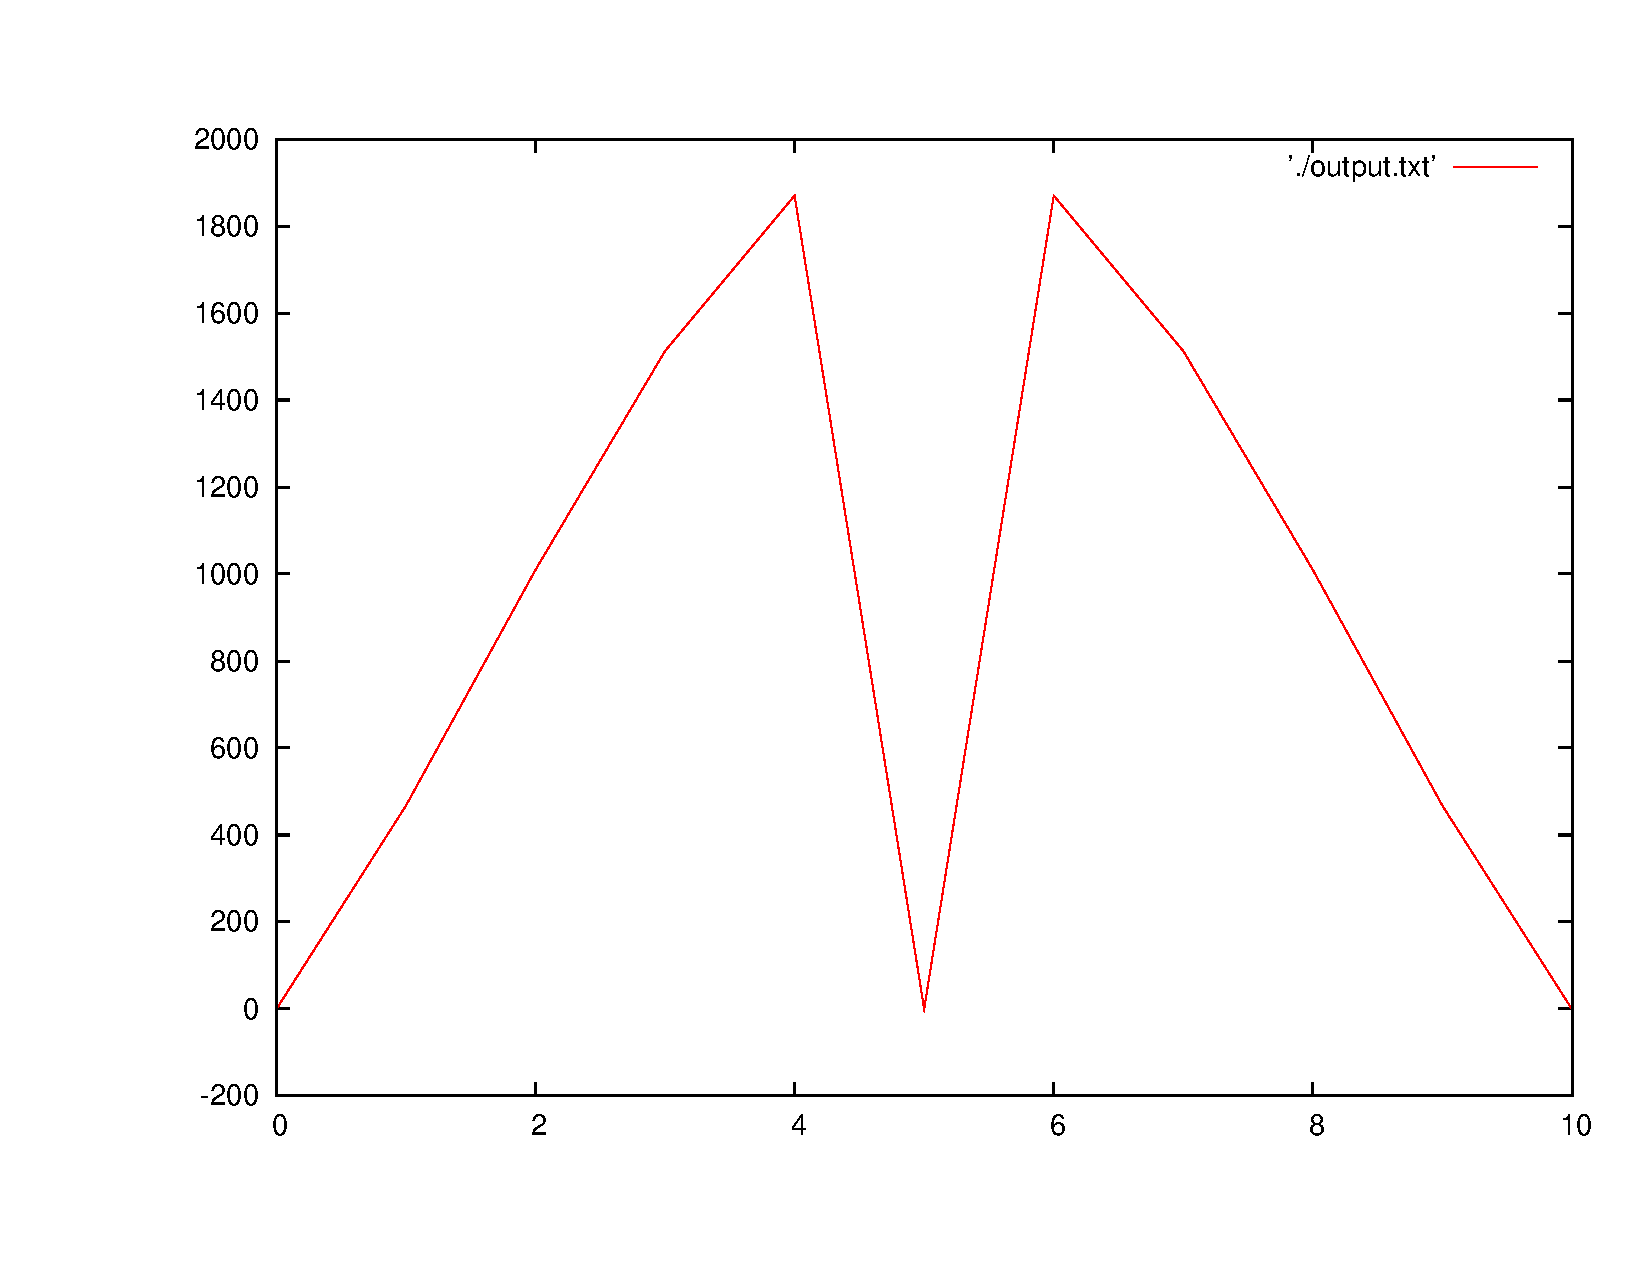
\includegraphics[width=.8\textwidth]{tms320c3x/fig_lp_output.pdf}
		\caption{\label{fig:tms320c3x_manual_lp_output} LP (Lowpass Finite Filter) output plot.}
	\end{center}
\end{figure}

This benchmark performs the computation of a LowPass Finite (LP) Filter over a digital signal.
The LP Filter is programmed in assembler using the \textit{z-transform}, which is widely utilized for the analysis of discrete-time signals, simular to the Laplace transform for continuous-time signals.
The implementation is based on the algorithm description provided in ``\textit{Digital Signal Processing: Laboratory Experiments Using C and the TMS320C31 DSK}'' book by Rulph Chassaing (1999, John Wiley \& Sons, Inc.).

The benchmark is mainly written in assembler, and it has been modified to accept an input signal within the ``\texttt{input\_signal.txt}'' file, to automatically compute the coefficients depending on the input signal length and to generate an output on the ``\texttt{output.txt}'' file.

This benchmark has been selected to globally check the sequential behavior of floating point instructions and the parallel floating point instructions.

This benchmark requires the TI C I/O service enabled to run in the TMS320C3X simulator.
A precompiled binary (\texttt{bp45.out}) is provided together with a GNU Make compatible Makefile.
A simulation configuration file (\texttt{sim\_config.xml}) for this benchmark is also provided, so that the simulator can run the benchmark with the following command:
  
\begin{verbatim}
$ unisim-tms320c3x-2.0 -c sim_config.xml
\end{verbatim}

The expected output data set is in the \texttt{output.ref.txt} file.
You can use plotting tools like \textit{gnuplot} to plot the generated output. 

Figure~\ref{fig:tms320c3x_manual_lp_output} shows the plot of \texttt{output.txt} using the following command under \textit{gnuplot}:

\begin{verbatim}
gnuplot > plot './output.txt' with lines
\end{verbatim}

\subsubsection{BP (Bandpass Finite Filter)}
\label{tms320c3x_sec:benchmarks_bp}

\begin{figure}[!h]
	\begin{center}
		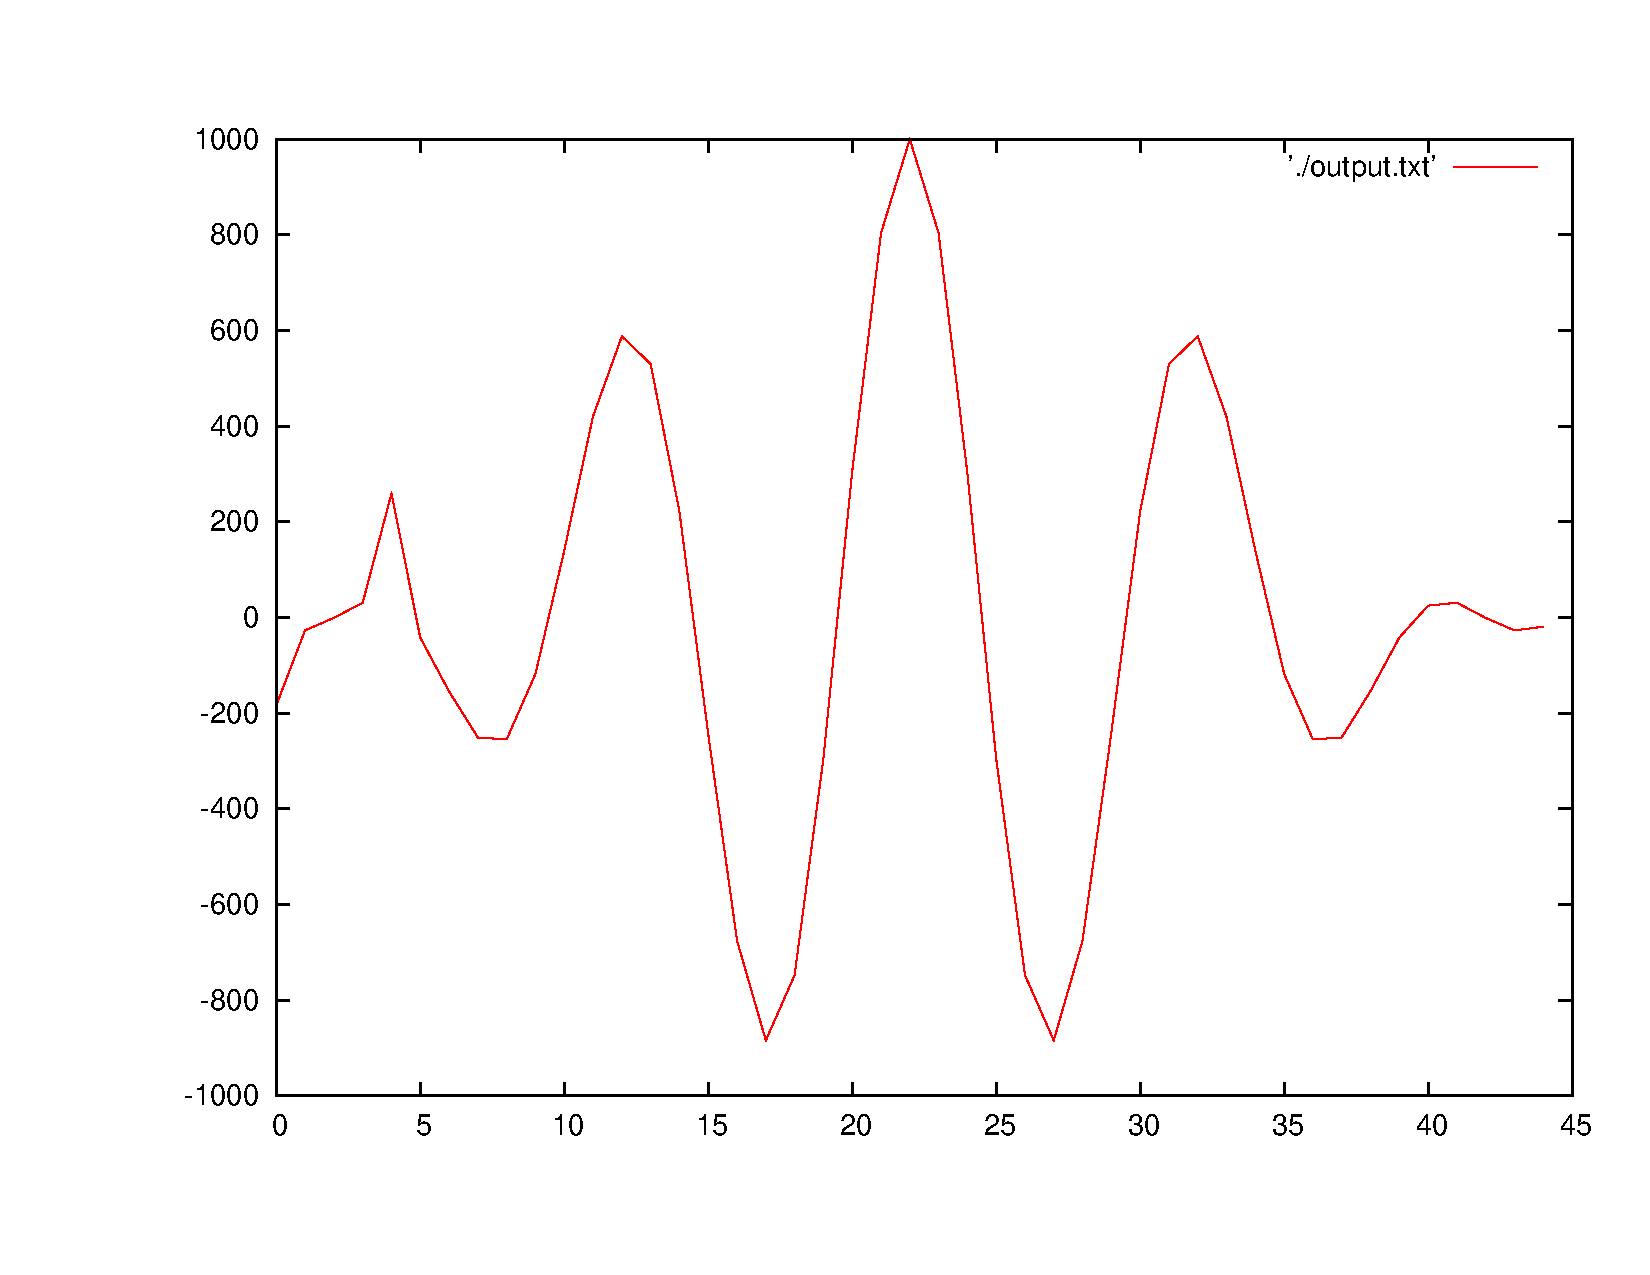
\includegraphics[width=.8\textwidth]{tms320c3x/fig_bp_output.pdf}
		\caption{\label{fig:tms320c3x_manual_bp_output} BP (Bandpass Finite Filter) output plot.}
	\end{center}
\end{figure}

This benchmark performs the computation of a BandPass Finite (LP) Filter over a digital signal.
The LP Filter is programmed in assembler using the \textit{z-transform}, which is widely utilized for the analysis of discrete-time signals, simular to the Laplace transform for continuous-time signals.
The implementation is based on the algorithm description provided in ``\textit{Digital Signal Processing: Laboratory Experiments Using C and the TMS320C31 DSK}'' book by Rulph Chassaing (1999, John Wiley \& Sons, Inc.).
The benchmark is mainly written in assembler, and it has been modified to accept an input signal (only 45 coefficients are considered) within the ``\texttt{input\_signal.txt}'' file, and to generate an output on the ``\texttt{output.txt}'' file.

As for the LowPass filter benchmark, this benchmark has been selected to globally check the sequential behavior of floating point instructions and some parallel floating point instructions.

This benchmark requires the TI C I/O service enabled to run in the TMS320C3X simulator.
A precompiled binary (\texttt{bp45.out}) is provided together with a GNU Make compatible Makefile.
A simulation configuration file (\texttt{sim\_config.xml}) for this benchmark is also provided, so that the simulator can run the benchmark with the following command:
  
\begin{verbatim}
$ unisim-tms320c3x-2.0 -c sim_config.xml
\end{verbatim}

The expected output data set is in the \texttt{output.ref.txt} file.
You can use plotting tools like \textit{gnuplot} to plot the generated output. 

Figure~\ref{fig:tms320c3x_manual_bp_output} shows the plot of \texttt{output.txt} using the following command under \textit{gnuplot}:

\begin{verbatim}
gnuplot > plot './output.txt' with lines
\end{verbatim}

\subsubsection{IIR (Biquad Infinite Filter)}

\begin{figure}[!h]
	\begin{center}
		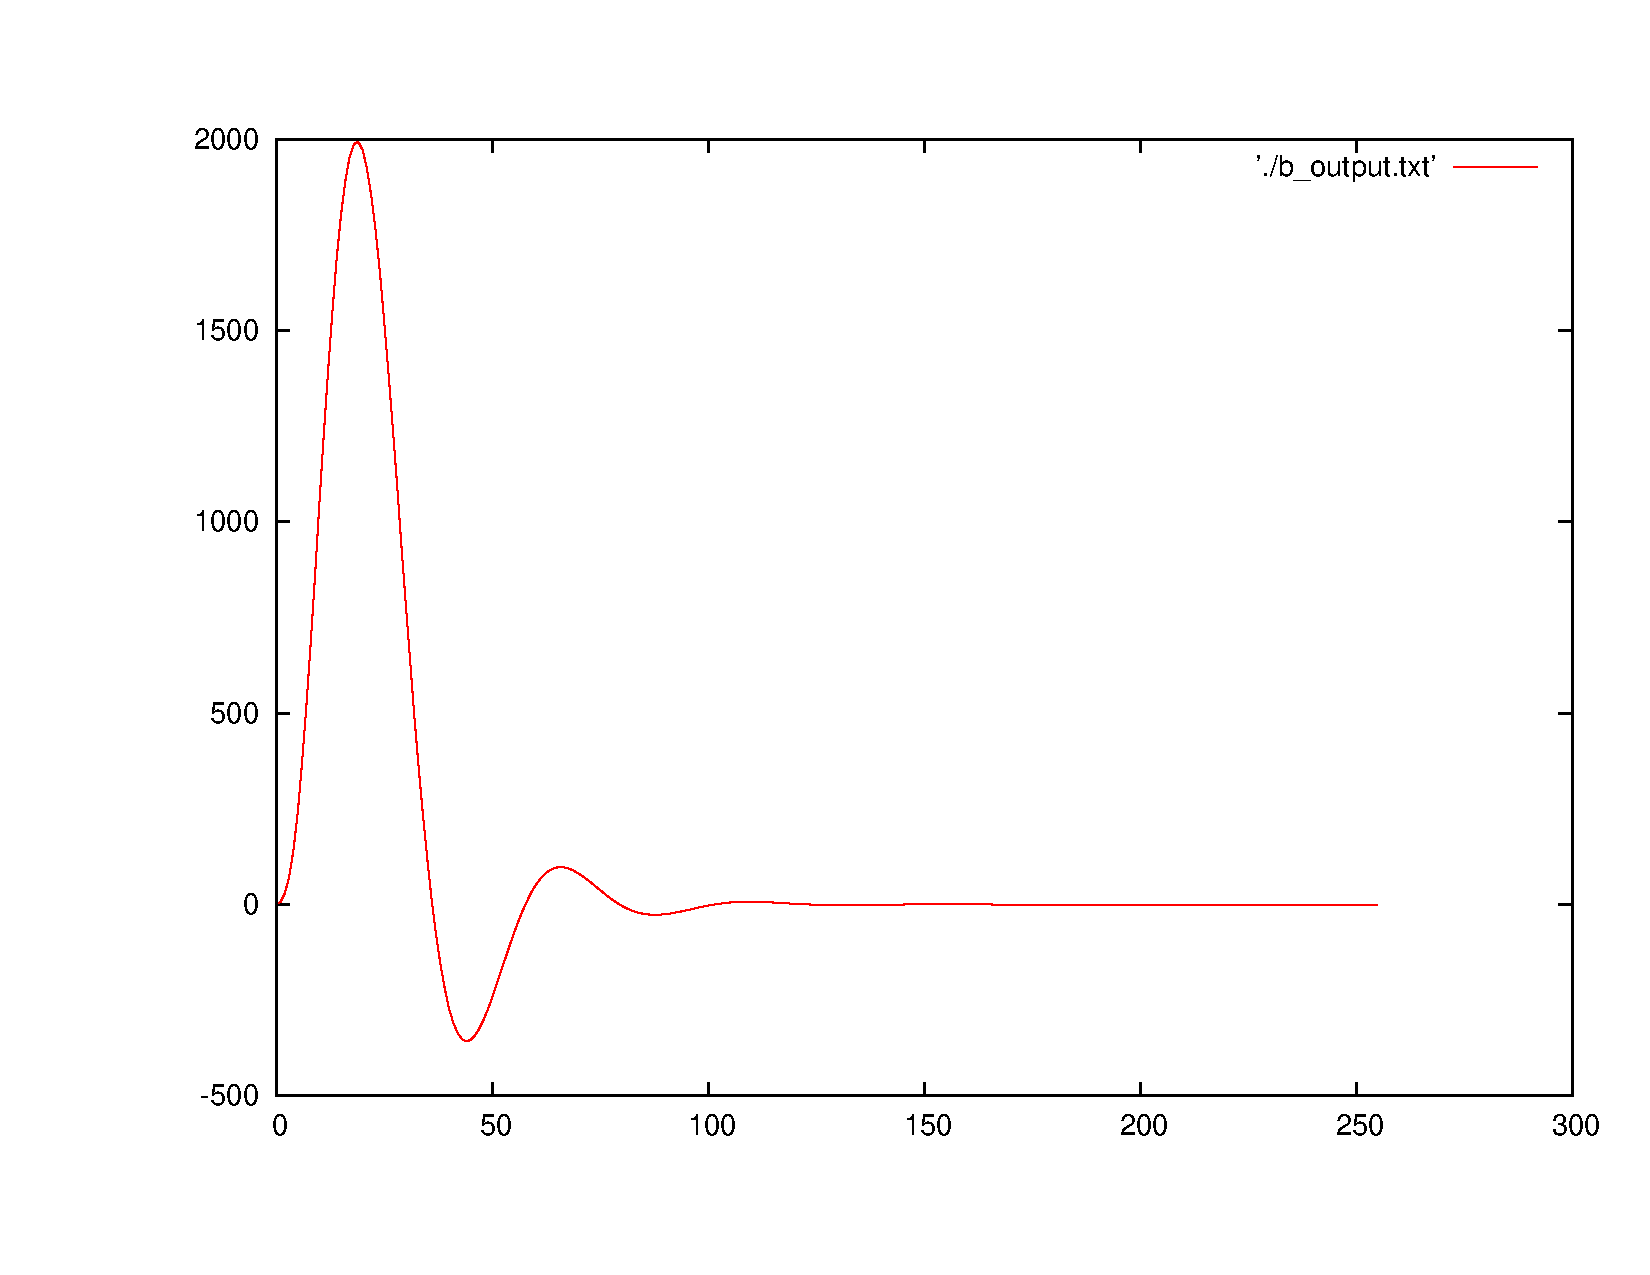
\includegraphics[width=.8\textwidth]{tms320c3x/fig_iir_output.pdf}
		\caption{\label{fig:tms320c3x_manual_iir_output}Plot of the IIR program using \textit{gnuplot}.}
	\end{center}
\end{figure}

This benchmarks performs the computation of an Infinite Impulse Response (IIR) Filter.
The previous filter benchmarks (see Sections~\ref{tms320c3x_sec:benchmarks_lp} and~\ref{tms320c3x_sec:benchmarks_bp}) do not have analog counterpart.
This filter benchmark makes use of the vast knowledge already acquired with analog filters.
The design procedure involves the conversion of an analog filter to an equivalent discrete filter using the bilinear transformation (BLT) technique.
As such, the BLT procedure converts a transfer function of an analog filter in the \textit{s}-domain into an equivalent discrete-time transfer function in the \textit{z}-domain.

This benchmark is based on two implementations of the biquad algorithm provided by the TI DSK 3 for the TMS320C3x.
The first implementation is done in pure C and uses floating point computation, and the second one is a fast version of the biquad algorithm programmed in assembler.
The benchmark provides at the end two different outputs, \texttt{b\_output.txt} for the C implementation and \texttt{fb\_output.txt} for the implementation in assembler.
Both outputs should be the same.

The IIR benchmark has been selected for the following reasons:
\begin{enumerate}
	\item It serves to check the correct sequential behavior of programs with an important use of floating point computations.
	\item It tests both floating point computations as generated by the TI C compiler and assembler code, which uses specialized instructions as parallel float computations.
	\item It tests complex addressing modes and specially the fast biquad implementation uses bit reverse addressing mode.
\end{enumerate}

This benchmark requires the TI C I/O service enabled to run in the TMS320C3X simulator.
A precompiled binary (\texttt{biquad4.out}) is provided together with a GNU Make compatible Makefile.
A simulation configuration file (\texttt{sim\_config.xml}) for this benchmark is also provided, so that the simulator can run the benchmark with the following command:
  
\begin{verbatim}
$ unisim-tms320c3x-2.0 -c sim_config.xml
\end{verbatim}

The expected output data set is in the \texttt{b\_output.ref.txt} and \texttt{fb\_output.ref.txt} files.
You can use plotting tools like \textit{gnuplot} to plot the generated outputs. 

Figure~\ref{fig:tms320c3x_manual_iir_output} shows the plot of \texttt{b\_output.txt} using the following command under \textit{gnuplot}:

\begin{verbatim}
gnuplot > plot './b_output.txt' with lines
\end{verbatim}

\subsubsection{FFT (Fast Fourier Transform)}

\begin{figure}[!h]
	\begin{center}
		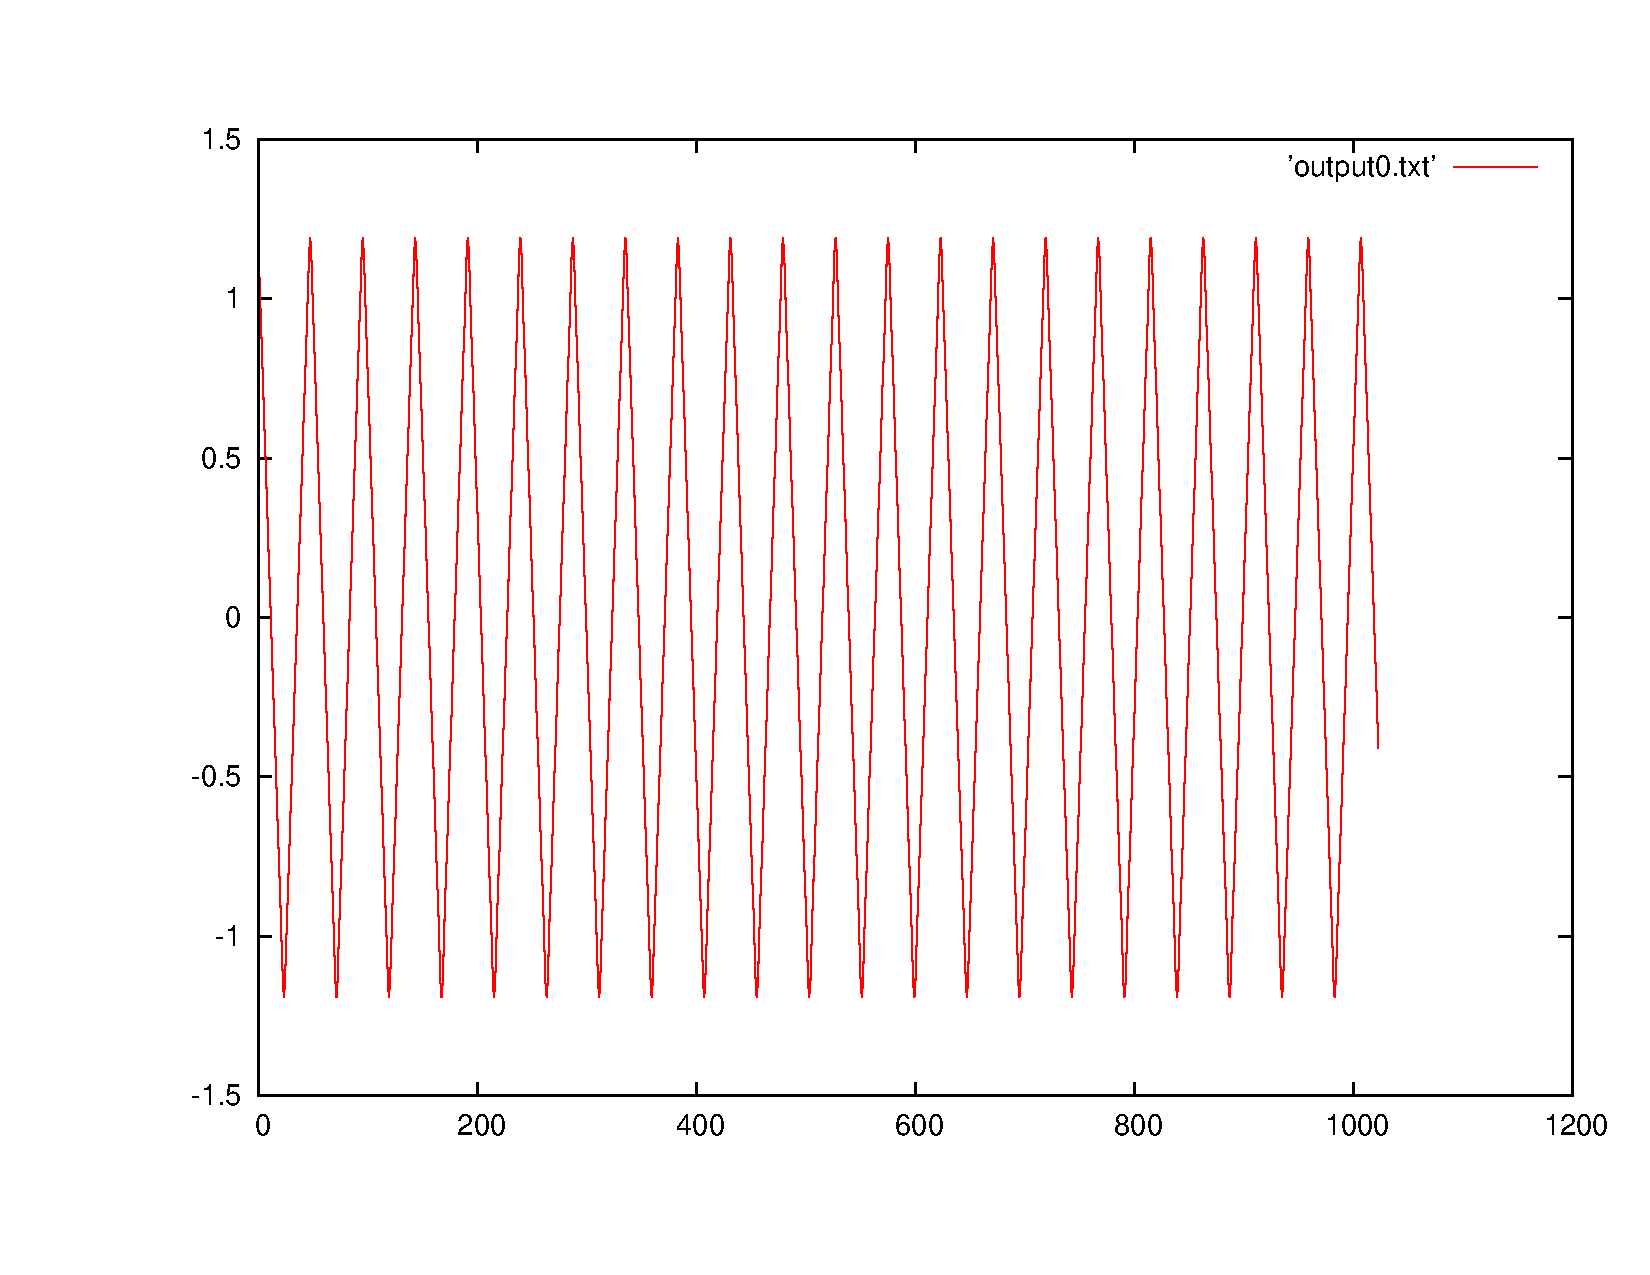
\includegraphics[width=.8\textwidth]{tms320c3x/fig_fft512_output0.pdf}
		\caption{\label{fig:tms320c3x_manual_fft_output0}Plot of the FFT512 program first iteration using \textit{gnuplot}.}
	\end{center}
\end{figure}

This benchmark simply computes a 512-point FFT (Fast Fourier Transform) using a Complex Radix 2 given a signal input.
It is based on the FFT codes provided by the TI DSK 3 for the TMS320C3x, modified to accept an input signal described as frequency and amplitude in two different input files: \textit{freq\_input.txt} (for the frequency) and \textit{ampl\_input.txt} (for the amplitude).
The benchmarks performs ten FFT iterations over the input signal and generates an output file for each of the iterations (\textit{output*.txt}, where ``*'' is the iteration number).

The FFT benchmark has been selected for the following reasons:
\begin{enumerate}
	\item As for the other floating point benchmarks it serves to check the correct sequential behavior of programs with an important use of floating point computations.
	\item Most of the program is written in assembler, using parallel float instructions that would otherwise have not been tested by the C compiler.
	\item The used FFT assembler implementation uses the bit reverse addressing mode, which is particularly well suited for FFT computations.
\end{enumerate} 

This benchmark requires the TI C I/O service enabled to run in the TMS320C3X simulator.
A precompiled binary (\texttt{fft.out}) is provided together with a GNU Make compatible Makefile.
A simulation configuration file (\texttt{sim\_config.xml}) for this benchmark is also provided, so that the simulator can run the benchmark with the following command:

\begin{verbatim}
$ unisim-tms320c3x-2.0 -c sim_config.xml
\end{verbatim}

The expected output data set is in the following files: \texttt{output0.ref.txt}, \texttt{output1.ref.txt}, \texttt{output2.ref.txt}, \texttt{output3.ref.txt}, \texttt{output4.ref.txt}, \texttt{output5.ref.txt}, \texttt{output6.ref.txt}, \texttt{output7.ref.txt}, \texttt{output8.ref.txt}, and \texttt{output9.ref.txt}.
You can use plotting tools like \textit{gnuplot} to plot the generated outputs. 

Figure~\ref{fig:tms320c3x_manual_fft_output0} shows the plot of \texttt{output0.txt} using the following command under \textit{gnuplot}:

\begin{verbatim}
gnuplot > plot './output0.txt' with lines
\end{verbatim}

\subsection{Instruction level unit tests}

As explained in Section~\ref{tms320c3x_benchmarks}, although they have validated general operations of the UNISIM TMS320C3X simulator, both the integer and floating-point benchmarks have insufficiently covered the TMS320C3X instructions.
Extensive testings at the instruction level are essential to gain greater confidence in the UNISIM TMS320C3X simulator representativity.
This section presents the validation process of UNISIM TMS320C3X simulator at the instruction level.
A unit testing environment, in the form of a Makefile for GNU Make, has been developed to allow testing individual instructions for the UNISIM TMS320C3X simulator.
Testing an instruction involves writing some "glue" code (C and Assembly) around the instruction under test to provide it with the input operands read from the host filesystem, and to save instruction output operands into a file on the host filesystem, so that results of instruction under test can be observed and compared.
A unit test generator, that is part of the testing environment, automatically generates that "glue" code, making writing and maintaining the instruction level unit tests easier.

Section~\ref{tms320c3x_validation_process} presents the validation process and the test plan.
Section~\ref{tms320c3x_testing_status} contains the testing status at instruction level of UNISIM TMS320C3X simulator.
Section~\ref{tms320c3x_unit_tests_generator} presents the unit tests generator flow.
Section~\ref{tms320c3x_testing_environment} presents the testing environment and Section~\ref{tms320c3x_regression_tests} shows how to use it as a regression test for the UNISIM TMS320C3X simulator.

\subsubsection{Validation process}
\label{tms320c3x_validation_process}

For the purpose of validating the UNISIM TMS320C3X simulator, a factorial plan has been established. 
The factorial plan parameters are:
\begin{itemize}
\item The general instruction under test, e.g. \texttt{ldf}, see Tables~\ref{table:tms320c3x_load_store_instructions}, \ref{table:tms320c3x_interlocked_instructions},  \ref{table:tms320c3x_control_instructions}, \ref{table:tms320c3x_2ops_instructions}, \ref{table:tms320c3x_3ops_instructions}, \ref{table:tms320c3x_parallel_instructions} and \ref{table:tms320c3x_power_instructions}
\item The condition code, e.g. \texttt{eq} in \texttt{ldfeq}, see Table~\ref{table:tms320c3x_condition_codes}
\item The general addressing mode (e.g. \texttt{indir} in \texttt{ldfeq indir, reg}), see Table~\ref{table:tms320c3x_general_addressing_modes}:
	\begin{itemize}
		\item For an immediate addressing mode, the immediate value
		\item For an indirect addressing mode, one of 26 available indirect addressing modes, see Table~\ref{table:tms320c3x_indir_addressing_modes}
	\end{itemize}
\item The input value set of the instruction, e.g. the value of \texttt{indir} memory operand in \texttt{ldfeq indir, reg}
\end{itemize}

\begin{table}[!p]
\begin{center}
	\small
	\begin{tabular}{|p{3.0cm}|p{10.0cm}|}
	\hline
	\textbf{Instructions} & \textbf{Description}\\
	\hline
	\textbf{lde} & Load Floating-Point Exponent\\
	\hline
	\textbf{ldf} & Load Floating-Point Value\\
	\hline
	\textbf{ldf\textit{cond}} & Load Floating-point Value Conditionally\\
	\hline
	\textbf{ldi} & Load Integer\\
	\hline
	\textbf{ldi\textit{cond}} & Load Integer Conditionally\\
	\hline
	\textbf{ldm} & Load Floating-Point Mantissa\\
	\hline
	\textbf{ldp} & Load Data-Page Pointer\\
	\hline
	\textbf{pop} & Pop Integer\\
	\hline
	\textbf{popf} & Pop Floating-Point Value\\
	\hline
	\textbf{push} & Push Integer\\
	\hline
	\textbf{pushf} & Push Floating-Point Value\\
	\hline
	\textbf{stf} & Store Floating-Point Value\\
	\hline
	\textbf{sti} & Store Integer\\
	\hline
	\end{tabular}
	\caption{\label{table:tms320c3x_load_store_instructions} TMS320C3X Load/Store Instructions.}
\end{center}
\end{table}

\begin{table}[!p]
\begin{center}
	\small
	\begin{tabular}{|p{3.0cm}|p{10.0cm}|}
	\hline
	\textbf{Instructions} & \textbf{Description}\\
	\hline
	\textbf{ldfi} & Load Floating-Point Value, Interlocked\\
	\hline
	\textbf{ldii} & Load Integer, Interlocked\\
	\hline
	\textbf{sigi} & Signal, Interlocked\\
	\hline
	\textbf{stfi} & Store Floating-Point Value, Interlocked\\
	\hline
	\textbf{stii} & Store Integer, Interlocked\\
	\hline
	\end{tabular}
	\caption{\label{table:tms320c3x_interlocked_instructions} TMS320C3X Interlocked Instructions.}
\end{center}
\end{table}

\begin{table}[!p]
\begin{center}
	\small
	\begin{tabular}{|p{3.0cm}|p{10.0cm}|}
	\hline
	\textbf{Instructions} & \textbf{Description}\\
	\hline
	\textbf{b\textit{cond}} & Branch Conditionally (Standard)\\
	\hline
	\textbf{b\textit{cond}d} & Branch Conditionally (Delayed)\\
	\hline
	\textbf{br} & Branch Unconditionally (Standard)\\
	\hline
	\textbf{brd} & Branch Unconditionally (Delayed)\\
	\hline
	\textbf{call} & Call Subroutine\\
	\hline
	\textbf{call\textit{cond}} & Call Subroutine Conditionally\\
	\hline
	\textbf{db\textit{cond}} & Decrement and Branch Conditionally (Standard)\\
	\hline
	\textbf{db\textit{cond}d} & Decrement and Branch Conditionally (Delayed)\\
	\hline
	\textbf{iack} & Interrupt Acknowledge\\
	\hline
	\textbf{idle} & Idle Until Interrupt\\
	\hline
	\textbf{nop} & No Operation\\
	\hline
	\textbf{reti\textit{cond}} & Return From Interrupt Conditionally\\
	\hline
	\textbf{rets\textit{cond}} & Return From Subroutine Conditionally\\
	\hline
	\textbf{rptb} & Repeat Block\\
	\hline
	\textbf{rpts} & Repeat Single Instruction\\
	\hline
	\textbf{swi} & Software Interrupt\\
	\hline
	\textbf{trap\textit{cond}} & Trap Conditionally\\
	\hline
	\end{tabular}
	\caption{\label{table:tms320c3x_control_instructions} TMS320C3X Control Instructions.}
\end{center}
\end{table}

\begin{table}[!p]
\begin{center}
	\small
	\begin{tabular}{|p{3.0cm}|p{10.0cm}|}
	\hline
	\textbf{Instructions} & \textbf{Description}\\
	\hline
	\textbf{absf} & Absolute Value of Floating-Point\\
	\hline
	\textbf{absi} & Absolute Value of Integer\\
	\hline
	\textbf{addc} & Add Integer With Carry\\
	\hline
	\textbf{addf} & Add Floating-Point Values\\
	\hline
	\textbf{addi} & Add Integer\\
	\hline
	\textbf{and} & Bitwise-Logical AND\\
	\hline
	\textbf{andn} & Bitwise-Logical AND With Complement\\
	\hline
	\textbf{ash} & Arithmetic Shift\\
	\hline
	\textbf{cmpf} & Compare Floating-Point Value\\
	\hline
	\textbf{cmpi} & Compare Integer\\
	\hline
	\textbf{fix} & Floating-Point-to-Integer Conversion\\
	\hline
	\textbf{float} & Integer-to-Floating-Point Conversion\\
	\hline
	\textbf{lsh} & Logical Shift\\
	\hline
	\textbf{mpyf} & Multiply Floating-Point Value\\
	\hline
	\textbf{mpyi} & Multiply Integer\\
	\hline
	\textbf{negb} & Negative Integer With Borrow\\
	\hline
	\textbf{negf} & Negative Floating-Point Value\\
	\hline
	\textbf{negi} & Negate Integer\\
	\hline
	\textbf{norm} & Normalize\\
	\hline
	\textbf{not} & Bitwise-Logical Complement\\
	\hline
	\textbf{or} & Bitwise-Logical OR\\
	\hline
	\textbf{rnd} & Round Floating-Point Value\\
	\hline
	\textbf{rol} & Rotate Left\\
	\hline
	\textbf{rolc} & Rotate Left Through Carry\\
	\hline
	\textbf{ror} & Rotate Right\\
	\hline
	\textbf{rorc} & Rotate Right Through Carry\\
	\hline
	\textbf{subb} & Substract Integer With Borrow\\
	\hline
	\textbf{subc} & Substract Integer Conditionally\\
	\hline
	\textbf{subf} & Substract Floating-Point Value\\
	\hline
	\textbf{subi} & Substract Integer\\
	\hline
	\textbf{subrb} & Substract Reverse Integer With Borrow\\
	\hline
	\textbf{subrf} & Substract Reverse Floating-Point Value\\
	\hline
	\textbf{subri} & Substract Reverse Integer\\
	\hline
	\textbf{tstb} & Test Bit Fields\\
	\hline
	\textbf{xor} & Bitwise-Exclusive OR\\
	\hline
	\end{tabular}
	\caption{\label{table:tms320c3x_2ops_instructions} TMS320C3X 2-operand Instructions.}
\end{center}
\end{table}

\begin{table}[!p]
\begin{center}
	\small
	\begin{tabular}{|p{3.0cm}|p{10.0cm}|}
	\hline
	\textbf{Instructions} & \textbf{Description}\\
	\hline
	\textbf{addc3} & Add Integer With Carry, 3-Operand\\
	\hline
	\textbf{addf3} & Add Floating-Point, 3-Operand\\
	\hline
	\textbf{addi3} & Add Integer, 3-Operand\\
	\hline
	\textbf{and3} & Bitwise-Logical AND, 3-Operand\\
	\hline
	\textbf{andn3} & Bitwise-Logical AND With Complement, 3-Operand\\
	\hline
	\textbf{ash3} & Arithmetic Shift, 3-Operand\\
	\hline
	\textbf{cmpf3} & Compare Floating-Point Value, 3-Operand\\
	\hline
	\textbf{cmpi3} & Compare Integer, 3-Operand\\
	\hline
	\textbf{lsh3} & Logical Shift, 3-Operand\\
	\hline
	\textbf{mpyf3} & Multiply Floating-Point Value, 3-Operand\\
	\hline
	\textbf{mpyi3} & Multiply Integer, 3-Operand\\
	\hline
	\textbf{or3} & Bitwise-Logical OR, 3-Operand\\
	\hline
	\textbf{subb3} & Substract Integer With Borrow, 3-Operand\\
	\hline
	\textbf{subf3} & Substract Floating-Point Value, 3-Operand\\
	\hline
	\textbf{subi3} & Substract Integer, 3-Operand\\
	\hline
	\textbf{tstb3} & Test Bit Fields, 3-Operand\\
	\hline
	\textbf{xor3} & Bitwise-Exclusive OR, 3-Operand\\
	\hline
	\end{tabular}
	\caption{\label{table:tms320c3x_3ops_instructions} TMS320C3X 3-operand Instructions.}
\end{center}
\end{table}

\begin{table}[!p]
\begin{center}
	\small
	\begin{tabular}{|p{3.0cm}|p{10.0cm}|}
	\hline
	\textbf{Instructions} & \textbf{Description}\\
	\hline
	\textbf{absf}\texttt{~||~}\textbf{stf} & Parallel absf and stf\\
	\hline
	\textbf{absi}\texttt{~||~}\textbf{sti} & Parallel absi and sti\\
	\hline
	\textbf{addf3}\texttt{~||~}\textbf{stf} & Parallel addf3 and stf\\
	\hline
	\textbf{addi3}\texttt{~||~}\textbf{sti} & Parallel addi3 and sti\\
	\hline
	\textbf{and3}\texttt{~||~}\textbf{sti} & Parallel and3 and sti\\
	\hline
	\textbf{ash3}\texttt{~||~}\textbf{sti} & Parallel ash3 and sti\\
	\hline
	\textbf{fix}\texttt{~||~}\textbf{sti} & Parallel fix and sti\\
	\hline
	\textbf{float}\texttt{~||~}\textbf{sti} & Parallel float and stf\\
	\hline
	\textbf{ldf}\texttt{~||~}\textbf{ldf} & Parallel ldf and ldf\\
	\hline
	\textbf{ldf}\texttt{~||~}\textbf{stf} & Parallel ldf and stf\\
	\hline
	\textbf{ldi}\texttt{~||~}\textbf{ldi} & Parallel ldi and ldi\\
	\hline
	\textbf{ldi}\texttt{~||~}\textbf{sti} & Parallel ldi and sti\\
	\hline
	\textbf{lsh3}\texttt{~||~}\textbf{sti} & Parallel lsh3 and sti\\
	\hline
	\textbf{mpyf3}\texttt{~||~}\textbf{addf3} & Parallel mpyf3 and addf3\\
	\hline
	\textbf{mpyf3}\texttt{~||~}\textbf{stf} & Parallel mpyf3 and stf\\
	\hline
	\textbf{mpyf3}\texttt{~||~}\textbf{subf3} & Parallel mpyf3 and subf3\\
	\hline
	\textbf{mpyi3}\texttt{~||~}\textbf{addi3} & Parallel mpyi3 and addi3\\
	\hline
	\textbf{mpyi3}\texttt{~||~}\textbf{sti} & Parallel mpyi3 and sti\\
	\hline
	\textbf{mpyi3}\texttt{~||~}\textbf{subi3} & Parallel mpyi3 and subi3\\
	\hline
	\textbf{negf}\texttt{~||~}\textbf{stf} & Parallel negf and stf\\
	\hline
	\textbf{negi}\texttt{~||~}\textbf{sti} & Parallel negi and sti\\
	\hline
	\textbf{not}\texttt{~||~}\textbf{sti} & Parallel not and sti\\
	\hline
	\textbf{or3}\texttt{~||~}\textbf{sti} & Parallel or3 and sti\\
	\hline
	\textbf{stf}\texttt{~||~}\textbf{stf} & Parallel Store Floating-Point Value\\
	\hline
	\textbf{sti}\texttt{~||~}\textbf{sti} & Parallel sti and sti\\
	\hline
	\textbf{subf3}\texttt{~||~}\textbf{stf} & Parallel subf3 and stf\\
	\hline
	\textbf{subi3}\texttt{~||~}\textbf{sti} & Parallel subi3 and sti\\
	\hline
	\textbf{xor3}\texttt{~||~}\textbf{sti} & Parallel xor3 and sti\\
	\hline
	\end{tabular}
	\caption{\label{table:tms320c3x_parallel_instructions} TMS320C3X Parallel Instructions.}
\end{center}
\end{table}

\begin{table}[!p]
\begin{center}
	\small
	\begin{tabular}{|p{3.0cm}|p{10.0cm}|}
	\hline
	\textbf{Instructions} & \textbf{Description}\\
	\hline
	\textbf{idle2} & Low-Power Idle\\
	\hline
	\textbf{lopower} & Divide Clock by 16\\
	\hline
	\textbf{maxspeed} & Restore Clock to Regular Speed\\
	\hline
	\end{tabular}
	\caption{\label{table:tms320c3x_power_instructions} TMS320C3X Parallel Instructions.}
\end{center}
\end{table}

\begin{table}[!p]
\begin{center}
	\small
	\begin{tabular}{|p{3.0cm}|p{10.0cm}|}
	\hline
	\textbf{Condition codes (20)} & \textbf{Description}\\
	\hline
	\texttt{u} & unconditional \\
	\hline
	\texttt{lo} & lower than\\
	\hline
	\texttt{ls} & lower than or same as\\
	\hline
	\texttt{hi} & higher than\\
	\hline
	\texttt{hs} & higher than or same as\\
	\hline
	\texttt{eq} & equal\\
	\hline
	\texttt{ne} & not equal\\
	\hline
	\texttt{lt} & less than\\
	\hline
	\texttt{le} & less than or equal\\
	\hline
	\texttt{gt} & greater than\\
	\hline
	\texttt{ge} & greater than or equal\\
	\hline
	\texttt{nv} & no overflow\\
	\hline
	\texttt{v} & overflow\\
	\hline
	\texttt{nuf} & no floating-point underflow\\
	\hline
	\texttt{uf} & floating-point underflow\\
	\hline
	\texttt{nlv} & no overflow\\
	\hline
	\texttt{lv} & overflow\\
	\hline
	\texttt{nluf} & no latched floating-point underflow\\
	\hline
	\texttt{luf} & latched floating-point underflow\\
	\hline
	\texttt{zuf} & zero or floating-point underflow\\
	\hline
	\end{tabular}
	\caption{\label{table:tms320c3x_condition_codes} Condition codes.}
\end{center}
\end{table}

\begin{table}[!p]
\begin{center}
	\small
	\begin{tabular}{|p{3.0cm}|p{12.0cm}|}
	\hline
	\textbf{General\newline Addressing \newline Modes (4)} & \textbf{Description}\\
	\hline
	reg & register addressing mode\\
	\hline
	dir & direct addressing mode\\
	\hline
	imm & immediate addressing mode\\
	\hline
	indir & indirect addressing mode (see table)\\
	\hline
	\end{tabular}
	\caption{\label{table:tms320c3x_general_addressing_modes} General addressing modes.}
\end{center}
\end{table}

\begin{table}[!p]
\begin{center}
	\small
	\begin{tabular}{|p{2.3cm}|p{2.3cm}|p{11.0cm}|}
	\hline
	\textbf{Indirect\newline Addressing \newline Modes (26)} & \textbf{Tests} & \textbf{Description}\\
	\hline
	\texttt{*+ar$_n$(disp)} & \texttt{*+ar$_n$(1)} & indirect addressing with predisplacement add\\
	\hline
	\texttt{*-ar$_n$(disp)} & \texttt{*-ar$_n$(1)} & indirect addressing with predisplacement subtract\\
	\hline
	\texttt{*++ar$_n$(disp)} & \texttt{*++ar$_n$(1)} & indirect addressing with predisplacement add and modify\\
	\hline
	\texttt{*--ar$_n$(disp)} & \texttt{*--ar$_n$(1)} & indirect addressing with predisplacement substract and modify\\
	\hline
	\texttt{*ar$_n$++(disp)} & \texttt{*ar$_n$++(1)} & indirect addressing with postdisplacement add and modify\\
	\hline
	\texttt{*ar$_n$--(disp)} & \texttt{*ar$_n$--(1)} & indirect addressing with postdisplacement substract and modify\\
	\hline
	\texttt{*ar$_n$++(disp)\%} & \texttt{*ar$_n$++(1)\%} \newline \texttt{bk} $\in$ \{4,5\} & indirect addressing with postdisplacement add and circular modify\\
	\hline
	\texttt{*ar$_n$(disp)\%} & \texttt{*ar$_n$(disp)\%} \newline \texttt{bk} $\in$ \{4,5\} & indirect addressing with postdisplacement substract and circular modify\\
	\hline
	\texttt{*+ar$_n$(ir0)} & \texttt{*+ar$_n$(ir0)} \newline \texttt{ir0} $\in$ [0,15] & indirect addressing with preindex (ir0) add\\
	\hline
	\texttt{*-ar$_n$(ir0)} & \texttt{*-ar$_n$(ir0)} \newline \texttt{ir0} $\in$ [0,15] & indirect addressing with preindex (ir0) substract\\
	\hline
	\texttt{*++ar$_n$(ir0)} & \texttt{*++ar$_n$(ir0)} \newline \texttt{ir0} $\in$ [0,15] & indirect addressing with preindex (ir0) add and modify\\
	\hline
	\texttt{*--ar$_n$(ir0)} & \texttt{*--ar$_n$(ir0)} \newline \texttt{ir0} $\in$ [0,15] & indirect addressing with preindex (ir0) substract and modify\\
	\hline
	\texttt{*ar$_n$++(ir0)} & \texttt{*ar$_n$++(ir0)} \newline \texttt{ir0} $\in$ [0,15] & indirect addressing with postindex (ir0) add and modify\\
	\hline
	\texttt{*ar$_n$--(ir0)} & \texttt{*ar$_n$--(ir0)} \newline \texttt{ir0} $\in$ [0,15] & indirect addressing with postindex (ir0) substract and modify\\
	\hline
	\texttt{*ar$_n$++(ir0)\%} & \texttt{*ar$_n$++(ir0)\%} \newline \texttt{ir0} $\in$ [0,15] \newline \texttt{bk} $\in$ \{4,5\} & indirect addressing with postindex (ir0) add and circular modify\\
	\hline
	\texttt{*ar$_n$--(ir0)\%} & \texttt{*ar$_n$--(ir0)\%} \newline \texttt{ir0} $\in$ [0,15] \newline \texttt{bk} $\in$ \{4,5\} & indirect addressing with postindex (ir0) substract and circular modify\\
	\hline
	\texttt{*+ar$_n$(ir1)} & \texttt{*+ar$_n$(ir1)} \newline \texttt{ir1} $\in$ [0,15] & indirect addressing with preindex (ir1) add\\
	\hline
	\texttt{*-ar$_n$(ir1)} & \texttt{*-ar$_n$(ir1)} \newline \texttt{ir1} $\in$ [0,15] & indirect addressing with preindex (ir1) substract\\
	\hline
	\texttt{*++ar$_n$(ir1)} & \texttt{*++ar$_n$(ir1)} \newline \texttt{ir1} $\in$ [0,15] & indirect addressing with preindex (ir1) add and modify\\
	\hline
	\texttt{*--ar$_n$(ir1)} & \texttt{*--ar$_n$(ir1)} \newline \texttt{ir1} $\in$ [0,15] & indirect addressing with preindex (ir1) substract and modify\\
	\hline
	\texttt{*ar$_n$++(ir1)} & \texttt{*ar$_n$++(ir1)} \newline \texttt{ir1} $\in$ [0,15] & indirect addressing with postindex (ir1) add and modify\\
	\hline
	\texttt{*ar$_n$--(ir1)} & \texttt{*ar$_n$--(ir1)} \newline \texttt{ir1} $\in$ [0,15] & indirect addressing with postindex (ir1) substract and modify\\
	\hline
	\texttt{*ar$_n$++(ir1)\%} & \texttt{*ar$_n$++(ir1)\%} \newline \texttt{ir1} $\in$ [0,15] \newline \texttt{bk} $\in$ \{4,5\} & indirect addressing with postindex (ir1) add and circular modify\\
	\hline
	\texttt{*ar$_n$--(ir1)\%} & \texttt{*ar$_n$--(ir1)\%} \newline \texttt{ir1} $\in$ [0,15] \newline \texttt{bk} $\in$ \{4,5\} & indirect addressing with postindex (ir1) substract and circular modify\\
	\hline
	\texttt{*ar$_n$} & \texttt{*ar$_n$} & indirect addressing\\
	\hline
	\texttt{*ar$_n$++(ir0)b} & \texttt{*ar$_n$++(ir0)b} \newline \texttt{ir1} $\in$ [0,15] & indirect addressing with postindex (ir0) add and bit-reversed modify\\
	\hline
	\end{tabular}
	\caption{\label{table:tms320c3x_indir_addressing_modes} Indirect addressing modes.}
\end{center}
\end{table}

\FloatBarrier

This plan results in lot of instruction alternatives being tested (several condition codes and addressing modes).
A full exploration of the factorial plan would have resulted in an unreasonable number of unit tests.
To limit the number of unit tests and to still achieve a good testing status, the following choices have been done:
\begin{itemize}
\item The amount of immediate addressing have been limited because each unit test of immediate addressing results in one program. The following integer values have been tested: \texttt{0}, \texttt{-1}, \texttt{+1}, \texttt{-32768}, or \texttt{+32767}. These integer values have a special role in most integer computations (neutral element, bound of integer immediate value \ldots). The following floating-point values have been tested: \texttt{0.0}, \texttt{1.0}, \texttt{-1.0}, \texttt{1.5}, \texttt{-1.5}, \texttt{$2.5594 \cdot 10^2$}, \texttt{$7.8125 \cdot 10^{-3}$}, \texttt{$-7.8163 \cdot 10^{-3}$}, \texttt{$-2.56 \cdot 10^2$}. These floating-point value have a special role in most floating-point computations (neutral element, smallest/largest positive/negative immediate floating-point values \ldots).
\item Condition codes have been varied exhaustively for conditional load/store and control instructions, see Table~\ref{table:tms320c3x_condition_codes}.
\item Each general addressing mode has been tested for load/store, control, 2-operand, 3-operand, and parallel instructions (note: some instructions allow only few of them), see Table~\ref{table:tms320c3x_general_addressing_modes}.
\item All of the 26 indirect addressing modes have been tested for load/store instructions and 2-operand instructions (28 tests per instructions), see Table~\ref{table:tms320c3x_indir_addressing_modes}.
\item Only one (\texttt{*ar$_n$}) of the 26 indirect addressing modes have been tested for 3-operand instructions and parallel instructions because testing all combinations of the 26 indirect addressing modes would have resulted in an unreasonable number of unit tests.
The rational behind this choice is that the instructions implementations in the UNISIM TMS320C3X simulator share the same source code for the indirect addressing modes.
\item 2-operand instructions with register addressing have been tested 10000 times with random inputs.
\item 3-operand instructions, load/store instructions, and parallel instructions with register, direct and indirect addressing modes have been tested 100 times with random inputs.
\item Additional tests have been written to check \texttt{ar$_n$} update ordering when instruction has several operands with indirect addressing mode, or when \texttt{ar$_n$} is both updated by an indirect addressing mode and the instruction itself.
\item Random input integer values have an uniform distribution. Table~\ref{table:tms320c3x_unit_test_float_distribution} shows the distribution for the floating point numbers. Some remarkable values (neutral, smallest/largest positive/negative floating-point values \ldots) have non-null probability of occurrence.
\end{itemize}

These choices still have resulted in 3757 unit test programs for a total of 694282 unit tests.

\subsubsection{Testing status}
\label{tms320c3x_testing_status}

\noindent The table below summarizes the testing status of all instructions. 
The total number of unit tests is shown and the detail for the computation of that number is explained between parenthesis.
$100_{rand}$ means 100 tests with random inputs.
$5_{imm}$ means 5 tests with immediate addressing. 
$20_{cond}$ means 20 tests for each condition codes. 
$28_{indir}$ means 28 tests for each 26 indirect addressing mode. 
$1_{indir}$ means only \texttt{ar$_n$} indirect addressing mode tested. 
$28_{isr}$ means 28 interrupt service routines tested. 
$1_{ar}$ means one test for \texttt{ar$_n$} update ordering.

\newpage

\begin{center}
\tablehead{\hline
\multicolumn{1}{|c|}{\textbf{Instruction}} & \multicolumn{1}{|c|}{\textbf{Tested?}} & \multicolumn{1}{|c|}{\textbf{Description}}\\
\hline}
\tabletail{\hline}
\begin{supertabular}{|p{7.0cm}|p{1.0cm}|p{7.0cm}|}
\multicolumn{3}{|c|}{\textbf{lde}}\\
\hline
\multicolumn{1}{|p{7.0 cm}|}{\scriptsize \texttt{lde reg, reg}} & \multicolumn{1}{p{1.0cm}|}{Yes} & \multicolumn{1}{p{7.0cm}|}{100 unit tests ($100_{rand}$)}\\
\hline
\multicolumn{1}{|p{7.0cm}|}{\scriptsize \texttt{lde dir, reg}} & \multicolumn{1}{p{1.0cm}|}{Yes} & \multicolumn{1}{p{7.0cm}|}{100 unit tests ($100_{rand}$)}\\
\hline
\multicolumn{1}{|p{7.0cm}|}{\scriptsize \texttt{lde indir, reg}} & \multicolumn{1}{p{1.0cm}|}{Yes} & \multicolumn{1}{p{7.0cm}|}{2800 unit tests ($28_{indir} \times 100_{rand}$)}\\
\hline
\multicolumn{1}{|p{7.0cm}|}{\scriptsize \texttt{lde imm, reg}} & \multicolumn{1}{p{1.0cm}|}{Yes} & \multicolumn{1}{p{7.0cm}|}{5 unit tests ($5_{imm}$)}\\
\hline
\multicolumn{3}{|c|}{\textbf{ldf}}\\
\hline
\multicolumn{1}{|p{7.0cm}|}{\scriptsize \texttt{ldf reg, reg}} & \multicolumn{1}{p{1.0cm}|}{Yes} & \multicolumn{1}{p{7.0cm}|}{100 unit tests ($100_{rand}$)}\\
\hline
\multicolumn{1}{|p{7.0cm}|}{\scriptsize \texttt{ldf dir, reg}} & \multicolumn{1}{p{1.0cm}|}{Yes} & \multicolumn{1}{p{7.0cm}|}{100 unit tests ($100_{rand}$)}\\
\hline
\multicolumn{1}{|p{7.0cm}|}{\scriptsize \texttt{ldf indir, reg}} & \multicolumn{1}{p{1.0cm}|}{Yes} & \multicolumn{1}{p{7.0cm}|}{2800 unit tests ($28_{indir} \times 100_{rand}$)}\\
\hline
\multicolumn{1}{|p{7.0cm}|}{\scriptsize \texttt{ldf imm, reg}} & \multicolumn{1}{p{1.0cm}|}{Yes} & \multicolumn{1}{p{7.0cm}|}{5 unit tests ($5_{imm}$)}\\
\hline
\multicolumn{3}{|c|}{\textbf{ldf\textit{cond}}}\\
\hline
\multicolumn{1}{|p{7.0cm}|}{\scriptsize \texttt{ldf\textit{cond} reg, reg}} & \multicolumn{1}{p{1.0cm}|}{Yes} & \multicolumn{1}{p{7.0cm}|}{2000 unit tests ($20_{cond} \times 100_{rand}$)}\\
\hline
\multicolumn{1}{|p{7.0cm}|}{\scriptsize \texttt{ldf\textit{cond} dir, reg}} & \multicolumn{1}{p{1.0cm}|}{Yes} & \multicolumn{1}{p{7.0cm}|}{2000 unit tests ($20_{cond} \times 100_{rand}$)}\\
\hline
\multicolumn{1}{|p{7.0cm}|}{\scriptsize \texttt{ldf\textit{cond} indir, reg}} & \multicolumn{1}{p{1.0cm}|}{Yes} & \multicolumn{1}{p{7.0cm}|}{56K unit tests ($28_{indir} \times 20_{cond} \times 100_{rand}$)}\\
\hline
\multicolumn{1}{|p{7.0cm}|}{\scriptsize \texttt{ldf\textit{cond} imm, reg}} & \multicolumn{1}{p{1.0cm}|}{Yes} & \multicolumn{1}{p{7.0cm}|}{100 unit tests ($100_{rand}$)}\\
\hline
\multicolumn{3}{|c|}{\textbf{ldi}}\\
\hline
\multicolumn{1}{|p{7.0cm}|}{\scriptsize \texttt{ldi reg, reg}} & \multicolumn{1}{p{1.0cm}|}{Yes} & \multicolumn{1}{p{7.0cm}|}{100 unit tests ($100_{rand}$)}\\
\hline
\multicolumn{1}{|p{7.0cm}|}{\scriptsize \texttt{ldi dir, reg}} & \multicolumn{1}{p{1.0cm}|}{Yes} & \multicolumn{1}{p{7.0cm}|}{100 unit tests ($100_{rand}$)}\\
\hline
\multicolumn{1}{|p{7.0cm}|}{\scriptsize \texttt{ldi indir, reg}} & \multicolumn{1}{p{1.0cm}|}{Yes} & \multicolumn{1}{p{7.0cm}|}{2900 unit tests ($(28_{indir} + 1_{ar}) \times 100_{rand}$)}\\
\hline
\multicolumn{1}{|p{7.0cm}|}{\scriptsize \texttt{ldi imm, reg}} & \multicolumn{1}{p{1.0cm}|}{Yes} & \multicolumn{1}{p{7.0cm}|}{5 unit tests ($5_{imm}$)}\\
\hline
\multicolumn{3}{|c|}{\textbf{ldi\textit{cond}}}\\
\hline
\multicolumn{1}{|p{7.0cm}|}{\scriptsize \texttt{ldi\textit{cond} reg, reg}} & \multicolumn{1}{p{1.0cm}|}{Yes} & \multicolumn{1}{p{7.0cm}|}{2000 unit tests ($20_{cond} \times 100_{rand}$)}\\
\hline
\multicolumn{1}{|p{7.0cm}|}{\scriptsize \texttt{ldi\textit{cond} dir, reg}} & \multicolumn{1}{p{1.0cm}|}{Yes} & \multicolumn{1}{p{7.0cm}|}{2000 unit tests ($20_{cond} \times 100_{rand}$)}\\
\hline
\multicolumn{1}{|p{7.0cm}|}{\scriptsize \texttt{ldi\textit{cond} indir, reg}} & \multicolumn{1}{p{1.0cm}|}{Yes} & \multicolumn{1}{p{7.0cm}|}{56K unit tests ($(28_{indir} + 1_{ar}) \times 20_{cond} \times 100_{rand}$)}\\
\hline
\multicolumn{1}{|p{7.0cm}|}{\scriptsize \texttt{ldi\textit{cond} imm, reg}} & \multicolumn{1}{p{1.0cm}|}{Yes} & \multicolumn{1}{p{7.0cm}|}{100 unit tests ($100_{rand}$)}\\
\hline
\multicolumn{3}{|c|}{\textbf{ldm}}\\
\hline
\multicolumn{1}{|p{7.0cm}|}{\scriptsize \texttt{ldm reg, reg}} & \multicolumn{1}{p{1.0cm}|}{Yes} & \multicolumn{1}{p{7.0cm}|}{100 unit tests ($100_{rand}$)}\\
\hline
\multicolumn{1}{|p{7.0cm}|}{\scriptsize \texttt{ldm dir, reg}} & \multicolumn{1}{p{1.0cm}|}{Yes} & \multicolumn{1}{p{7.0cm}|}{100 unit tests ($100_{rand}$)}\\
\hline
\multicolumn{1}{|p{7.0cm}|}{\scriptsize \texttt{ldm indir, reg}} & \multicolumn{1}{p{1.0cm}|}{Yes} & \multicolumn{1}{p{7.0cm}|}{2800 unit tests ($28_{indir} \times 100_{rand}$)}\\
\hline
\multicolumn{1}{|p{7.0cm}|}{\scriptsize \texttt{ldm imm, reg}} & \multicolumn{1}{p{1.0cm}|}{Yes} & \multicolumn{1}{p{7.0cm}|}{5 unit tests ($5_{imm}$)}\\
\hline
\multicolumn{3}{|c|}{\textbf{ldp}}\\
\hline
\multicolumn{1}{|p{7.0cm}|}{\scriptsize \texttt{ldp src}} & \multicolumn{1}{p{1.0cm}|}{Yes} & \multicolumn{1}{p{7.0cm}|}{Any benchmark and unit test}\\
\hline
\multicolumn{3}{|c|}{\textbf{pop}}\\
\hline
\multicolumn{1}{|p{7.0cm}|}{\scriptsize \texttt{pop reg}} & \multicolumn{1}{p{1.0cm}|}{Yes} & \multicolumn{1}{p{7.0cm}|}{Any benchmark and unit test}\\
\hline
\multicolumn{3}{|c|}{\textbf{popf}}\\
\hline
\multicolumn{1}{|p{7.0cm}|}{\scriptsize \texttt{popf reg}} & \multicolumn{1}{p{1.0cm}|}{Yes} & \multicolumn{1}{p{7.0cm}|}{Any floating-point benchmark and unit test}\\
\hline
\multicolumn{3}{|c|}{\textbf{push}}\\
\hline
\multicolumn{1}{|p{7.0cm}|}{\scriptsize \texttt{push reg}} & \multicolumn{1}{p{1.0cm}|}{Yes} & \multicolumn{1}{p{7.0cm}|}{Any benchmark and unit test}\\
\hline
\multicolumn{3}{|c|}{\textbf{pushf}}\\
\hline
\multicolumn{1}{|p{7.0cm}|}{\scriptsize \texttt{pushf reg}} & \multicolumn{1}{p{1.0cm}|}{Yes} & \multicolumn{1}{p{7.0cm}|}{Any floating-point benchmark and unit test}\\
\hline
\multicolumn{3}{|c|}{\textbf{stf}}\\
\hline
\multicolumn{1}{|p{7.0cm}|}{\scriptsize \texttt{stf reg, dir}} & \multicolumn{1}{p{1.0cm}|}{Yes} & \multicolumn{1}{p{7.0cm}|}{100 unit tests ($100_{rand}$)}\\
\hline
\multicolumn{1}{|p{7.0cm}|}{\scriptsize \texttt{stf reg, indir}} & \multicolumn{1}{p{1.0cm}|}{Yes} & \multicolumn{1}{p{7.0cm}|}{2800 unit tests ($28_{indir} \times 100_{rand}$)}\\
\hline
\multicolumn{3}{|c|}{\textbf{sti}}\\
\hline
\multicolumn{1}{|p{7.0cm}|}{\scriptsize \texttt{sti reg, dir}} & \multicolumn{1}{p{1.0cm}|}{Yes} & \multicolumn{1}{p{7.0cm}|}{100 unit tests ($100_{rand}$)}\\
\hline
\multicolumn{1}{|p{7.0cm}|}{\scriptsize \texttt{sti reg, indir}} & \multicolumn{1}{p{1.0cm}|}{Yes} & \multicolumn{1}{p{7.0cm}|}{2900 unit tests ($(28_{indir} + 1_{ar}) \times 100_{rand}$)}\\
\hline
\multicolumn{3}{|c|}{\textbf{ldfi}}\\
\hline
\multicolumn{1}{|p{7.0cm}|}{\scriptsize \texttt{ldfi dir, reg}} & \multicolumn{1}{p{1.0cm}|}{No} & \multicolumn{1}{p{7.0cm}|}{interlocked instruction behavior depends on environment}\\
\hline
\multicolumn{1}{|p{7.0cm}|}{\scriptsize \texttt{ldfi indir, reg}} & \multicolumn{1}{p{1.0cm}|}{No} & \multicolumn{1}{p{7.0cm}|}{Instruction behavior depends on environment}\\
\hline
\multicolumn{3}{|c|}{\textbf{ldii}}\\
\hline
\multicolumn{1}{|p{7.0cm}|}{\scriptsize \texttt{ldii dir, reg}} & \multicolumn{1}{p{1.0cm}|}{No} & \multicolumn{1}{p{7.0cm}|}{Instruction behavior depends on environment}\\
\hline
\multicolumn{1}{|p{7.0cm}|}{\scriptsize \texttt{ldii indir, reg}} & \multicolumn{1}{p{1.0cm}|}{No} & \multicolumn{1}{p{7.0cm}|}{Instruction behavior depends on environment}\\
\hline
\multicolumn{3}{|c|}{\textbf{sigi}}\\
\hline
\multicolumn{1}{|p{7.0cm}|}{\scriptsize \texttt{sigi}} & \multicolumn{1}{p{1.0cm}|}{No} & \multicolumn{1}{p{7.0cm}|}{Unimplemented. Instruction behavior depends on environment}\\
\hline
\multicolumn{3}{|c|}{\textbf{stfi}}\\
\hline
\multicolumn{1}{|p{7.0cm}|}{\scriptsize \texttt{stfi reg, dir}} & \multicolumn{1}{p{1.0cm}|}{No} & \multicolumn{1}{p{7.0cm}|}{Instruction behavior depends on environment}\\
\hline
\multicolumn{1}{|p{7.0cm}|}{\scriptsize \texttt{stfi reg, indir}} & \multicolumn{1}{p{1.0cm}|}{No} & \multicolumn{1}{p{7.0cm}|}{Instruction behavior depends on environment}\\
\hline
\multicolumn{3}{|c|}{\textbf{stii}}\\
\hline
\multicolumn{1}{|p{7.0cm}|}{\scriptsize \texttt{stii reg, dir}} & \multicolumn{1}{p{1.0cm}|}{No} & \multicolumn{1}{p{7.0cm}|}{Instruction behavior depends on environment}\\
\hline
\multicolumn{1}{|p{7.0cm}|}{\scriptsize \texttt{stii reg, indir}} & \multicolumn{1}{p{1.0cm}|}{No} & \multicolumn{1}{p{7.0cm}|}{Instruction behavior depends on environment}\\
\hline
\multicolumn{3}{|c|}{\textbf{b\textit{cond}}}\\
\hline
\multicolumn{1}{|p{7.0cm}|}{\scriptsize \texttt{b\textit{cond} reg}} & \multicolumn{1}{p{1.0cm}|}{Yes} & \multicolumn{1}{p{7.0cm}|}{2000 unit tests ($20_{cond} \times 100_{rand}$)}\\
\hline
\multicolumn{1}{|p{7.0cm}|}{\scriptsize \texttt{b\textit{cond} disp}} & \multicolumn{1}{p{1.0cm}|}{Yes} & \multicolumn{1}{p{7.0cm}|}{2000 unit tests ($20_{cond} \times 100_{rand}$)}\\
\hline
\multicolumn{3}{|c|}{\textbf{b\textit{cond}d}}\\
\hline
\multicolumn{1}{|p{7.0cm}|}{\scriptsize \texttt{b\textit{cond}d reg}} & \multicolumn{1}{p{1.0cm}|}{Yes} & \multicolumn{1}{p{7.0cm}|}{2000 unit tests ($20_{cond} \times 100_{rand}$)}\\
\hline
\multicolumn{1}{|p{7.0cm}|}{\scriptsize \texttt{b\textit{cond}d disp}} & \multicolumn{1}{p{1.0cm}|}{Yes} & \multicolumn{1}{p{7.0cm}|}{2000 unit tests ($20_{cond} \times 100_{rand}$)}\\
\hline
\multicolumn{3}{|c|}{\textbf{br}}\\
\hline
\multicolumn{1}{|p{7.0cm}|}{\scriptsize \texttt{br src}} & \multicolumn{1}{p{1.0cm}|}{Yes} & \multicolumn{1}{p{7.0cm}|}{100 unit tests ($100_{rand}$)}\\
\hline
\multicolumn{3}{|c|}{\textbf{brd}}\\
\hline
\multicolumn{1}{|p{7.0cm}|}{\scriptsize \texttt{brd src}} & \multicolumn{1}{p{1.0cm}|}{Yes} & \multicolumn{1}{p{7.0cm}|}{100 unit tests ($100_{rand}$)}\\
\hline
\multicolumn{3}{|c|}{\textbf{call}}\\
\hline
\multicolumn{1}{|p{7.0cm}|}{\scriptsize \texttt{call src}} & \multicolumn{1}{p{1.0cm}|}{Yes} & \multicolumn{1}{p{7.0cm}|}{100 unit tests ($100_{rand}$)}\\
\hline
\multicolumn{3}{|c|}{\textbf{call\textit{cond}}}\\
\hline
\multicolumn{1}{|p{7.0cm}|}{\scriptsize \texttt{call\textit{cond} reg}} & \multicolumn{1}{p{1.0cm}|}{Yes} & \multicolumn{1}{p{7.0cm}|}{2000 unit tests ($20_{cond} \times 100_{rand}$)}\\
\hline
\multicolumn{1}{|p{7.0cm}|}{\scriptsize \texttt{call\textit{cond} disp}} & \multicolumn{1}{p{1.0cm}|}{Yes} & \multicolumn{1}{p{7.0cm}|}{2000 unit tests ($20_{cond} \times 100_{rand}$)}\\
\hline
\multicolumn{3}{|c|}{\textbf{db\textit{cond}}}\\
\hline
\multicolumn{1}{|p{7.0cm}|}{\scriptsize \texttt{db\textit{cond} ar$_n$, reg}} & \multicolumn{1}{p{1.0cm}|}{Yes} & \multicolumn{1}{p{7.0cm}|}{2000 unit tests ($20_{cond} \times 100_{rand}$)}\\
\hline
\multicolumn{1}{|p{7.0cm}|}{\scriptsize \texttt{db\textit{cond} ar$_n$, disp}} & \multicolumn{1}{p{1.0cm}|}{Yes} & \multicolumn{1}{p{7.0cm}|}{2000 unit tests ($20_{cond} \times 100_{rand}$)}\\
\hline
\multicolumn{3}{|c|}{\textbf{db\textit{cond}d}}\\
\hline
\multicolumn{1}{|p{7.0cm}|}{\scriptsize \texttt{db\textit{cond}d ar$_n$, reg}} & \multicolumn{1}{p{1.0cm}|}{Yes} & \multicolumn{1}{p{7.0cm}|}{2000 unit tests ($20_{cond} \times 100_{rand}$)}\\
\hline
\multicolumn{1}{|p{7.0cm}|}{\scriptsize \texttt{db\textit{cond}d ar$_n$, disp}} & \multicolumn{1}{p{1.0cm}|}{Yes} & \multicolumn{1}{p{7.0cm}|}{2000 unit tests ($20_{cond} \times 100_{rand}$)}\\
\hline
\multicolumn{3}{|c|}{\textbf{iack}}\\
\hline
\multicolumn{1}{|p{7.0cm}|}{\scriptsize \texttt{iack dir}} & \multicolumn{1}{p{1.0cm}|}{No} & \multicolumn{1}{p{7.0cm}|}{Unimplemented. Instruction depends on circuitry}\\
\hline
\multicolumn{1}{|p{7.0cm}|}{\scriptsize \texttt{iack indir}} & \multicolumn{1}{p{1.0cm}|}{No} & \multicolumn{1}{p{7.0cm}|}{Unimplemented. Instruction depends on circuitry}\\
\hline
\multicolumn{3}{|c|}{\textbf{idle}}\\
\hline
\multicolumn{1}{|p{7.0cm}|}{\scriptsize \texttt{idle}} & \multicolumn{1}{p{1.0cm}|}{No} & \multicolumn{1}{p{7.0cm}|}{Instruction depends on external environment}\\
\hline
\multicolumn{3}{|c|}{\textbf{nop}}\\
\hline
\multicolumn{1}{|p{7.0cm}|}{\scriptsize \texttt{nop reg}} & \multicolumn{1}{p{1.0cm}|}{Yes} & \multicolumn{1}{p{7.0cm}|}{State does not change}\\
\hline
\multicolumn{1}{|p{7.0cm}|}{\scriptsize \texttt{nop indir}} & \multicolumn{1}{p{1.0cm}|}{Yes} & \multicolumn{1}{p{7.0cm}|}{State does not change}\\
\hline
\multicolumn{3}{|c|}{\textbf{reti\textit{cond}}}\\
\hline
\multicolumn{1}{|p{7.0cm}|}{\scriptsize \texttt{reti\textit{cond}}} & \multicolumn{1}{p{1.0cm}|}{Yes} & \multicolumn{1}{p{7.0cm}|}{2000 unit tests ($20_{cond} \times 100_{rand}$)}\\
\hline
\multicolumn{3}{|c|}{\textbf{rets\textit{cond}}}\\
\hline
\multicolumn{1}{|p{7.0cm}|}{\scriptsize \texttt{rets\textit{cond}}} & \multicolumn{1}{p{1.0cm}|}{Yes} & \multicolumn{1}{p{7.0cm}|}{2000 unit tests ($20_{cond} \times 100_{rand}$)}\\
\hline
\multicolumn{3}{|c|}{\textbf{rptb}}\\
\hline
\multicolumn{1}{|p{7.0cm}|}{\scriptsize \texttt{rptb src}} & \multicolumn{1}{p{1.0cm}|}{Yes} & \multicolumn{1}{p{7.0cm}|}{100 unit tests ($100_{rand}$)}\\
\hline
\multicolumn{3}{|c|}{\textbf{rpts}}\\
\hline
\multicolumn{1}{|p{7.0cm}|}{\scriptsize \texttt{rpts reg}} & \multicolumn{1}{p{1.0cm}|}{Yes} & \multicolumn{1}{p{7.0cm}|}{100 unit tests ($100_{rand}$)}\\
\hline
\multicolumn{1}{|p{7.0cm}|}{\scriptsize \texttt{rpts dir}} & \multicolumn{1}{p{1.0cm}|}{Yes} & \multicolumn{1}{p{7.0cm}|}{100 unit tests ($100_{rand}$)}\\
\hline
\multicolumn{1}{|p{7.0cm}|}{\scriptsize \texttt{rpts indir}} & \multicolumn{1}{p{1.0cm}|}{Yes} & \multicolumn{1}{p{7.0cm}|}{100 unit tests ($1_{indir} \times 100_{rand}$)}\\
\hline
\multicolumn{1}{|p{7.0cm}|}{\scriptsize \texttt{rpts imm}} & \multicolumn{1}{p{1.0cm}|}{Yes} & \multicolumn{1}{p{7.0cm}|}{1 unit tests ($1_{imm}$)}\\
\hline
\multicolumn{3}{|c|}{\textbf{swi}}\\
\hline
\multicolumn{1}{|p{7.0cm}|}{\scriptsize \texttt{swi}} & \multicolumn{1}{p{1.0cm}|}{No} & \multicolumn{1}{p{7.0cm}|}{Instruction depends on external environment}\\
\hline
\multicolumn{3}{|c|}{\textbf{trap\textit{cond}}}\\
\hline
\multicolumn{1}{|p{7.0cm}|}{\scriptsize \texttt{trap\textit{cond} n}} & \multicolumn{1}{p{1.0cm}|}{Yes} & \multicolumn{1}{p{7.0cm}|}{4800 unit tests (($20_{cond} \times 1_{isr} \times 100_{rand}) + (1_{cond} \times 28_{isr} \times 100_{rand})$)}\\
\hline
\multicolumn{3}{|c|}{\textbf{absf}}\\
\hline
\multicolumn{1}{|p{7.0cm}|}{\scriptsize \texttt{absf reg, reg}} & \multicolumn{1}{p{1.0cm}|}{Yes} & \multicolumn{1}{p{7.0cm}|}{10K unit tests ($10K_{rand}$)}\\
\hline
\multicolumn{1}{|p{7.0cm}|}{\scriptsize \texttt{absf dir, reg}} & \multicolumn{1}{p{1.0cm}|}{Yes} & \multicolumn{1}{p{7.0cm}|}{100 unit tests ($100_{rand}$)}\\
\hline
\multicolumn{1}{|p{7.0cm}|}{\scriptsize \texttt{absf indir, reg}} & \multicolumn{1}{p{1.0cm}|}{Yes} & \multicolumn{1}{p{7.0cm}|}{2800 unit tests ($28_{indir} \times 100_{rand}$)}\\
\hline
\multicolumn{1}{|p{7.0cm}|}{\scriptsize \texttt{absf imm, reg}} & \multicolumn{1}{p{1.0cm}|}{Yes} & \multicolumn{1}{p{7.0cm}|}{5 unit tests ($5_{imm}$)}\\
\hline
\multicolumn{3}{|c|}{\textbf{absi}}\\
\hline
\multicolumn{1}{|p{7.0cm}|}{\scriptsize \texttt{absi reg, reg}} & \multicolumn{1}{p{1.0cm}|}{Yes} & \multicolumn{1}{p{7.0cm}|}{10K unit tests ($10K_{rand}$)}\\
\hline
\multicolumn{1}{|p{7.0cm}|}{\scriptsize \texttt{absi dir, reg}} & \multicolumn{1}{p{1.0cm}|}{Yes} & \multicolumn{1}{p{7.0cm}|}{100 unit tests ($100_{rand}$)}\\
\hline
\multicolumn{1}{|p{7.0cm}|}{\scriptsize \texttt{absi indir, reg}} & \multicolumn{1}{p{1.0cm}|}{Yes} & \multicolumn{1}{p{7.0cm}|}{2900 unit tests ($(28_{indir} + 1_{ar}) \times 100_{rand}$)}\\
\hline
\multicolumn{1}{|p{7.0cm}|}{\scriptsize \texttt{absi imm, reg}} & \multicolumn{1}{p{1.0cm}|}{Yes} & \multicolumn{1}{p{7.0cm}|}{5 unit tests ($5_{imm}$)}\\
\hline
\multicolumn{3}{|c|}{\textbf{addc}}\\
\hline
\multicolumn{1}{|p{7.0cm}|}{\scriptsize \texttt{addc reg, reg}} & \multicolumn{1}{p{1.0cm}|}{Yes} & \multicolumn{1}{p{7.0cm}|}{10K unit tests ($10K_{rand}$)}\\
\hline
\multicolumn{1}{|p{7.0cm}|}{\scriptsize \texttt{addc dir, reg}} & \multicolumn{1}{p{1.0cm}|}{Yes} & \multicolumn{1}{p{7.0cm}|}{100 unit tests ($100_{rand}$)}\\
\hline
\multicolumn{1}{|p{7.0cm}|}{\scriptsize \texttt{addc indir, reg}} & \multicolumn{1}{p{1.0cm}|}{Yes} & \multicolumn{1}{p{7.0cm}|}{2900 unit tests ($(28_{indir} + 1_{ar}) \times 100_{rand}$)}\\
\hline
\multicolumn{1}{|p{7.0cm}|}{\scriptsize \texttt{addc imm, reg}} & \multicolumn{1}{p{1.0cm}|}{Yes} & \multicolumn{1}{p{7.0cm}|}{5 unit tests ($5_{imm}$)}\\
\hline
\multicolumn{3}{|c|}{\textbf{addf}}\\
\hline
\multicolumn{1}{|p{7.0cm}|}{\scriptsize \texttt{addf reg, reg}} & \multicolumn{1}{p{1.0cm}|}{Yes} & \multicolumn{1}{p{7.0cm}|}{10K unit tests ($10K_{rand}$)}\\
\hline
\multicolumn{1}{|p{7.0cm}|}{\scriptsize \texttt{addf dir, reg}} & \multicolumn{1}{p{1.0cm}|}{Yes} & \multicolumn{1}{p{7.0cm}|}{100 unit tests ($100_{rand}$)}\\
\hline
\multicolumn{1}{|p{7.0cm}|}{\scriptsize \texttt{addf indir, reg}} & \multicolumn{1}{p{1.0cm}|}{Yes} & \multicolumn{1}{p{7.0cm}|}{2800 unit tests ($28_{indir} \times 100_{rand}$)}\\
\hline
\multicolumn{1}{|p{7.0cm}|}{\scriptsize \texttt{addf imm, reg}} & \multicolumn{1}{p{1.0cm}|}{Yes} & \multicolumn{1}{p{7.0cm}|}{5 unit tests ($5_{imm}$)}\\
\hline
\multicolumn{3}{|c|}{\textbf{addi}}\\
\hline
\multicolumn{1}{|p{7.0cm}|}{\scriptsize \texttt{addi reg, reg}} & \multicolumn{1}{p{1.0cm}|}{Yes} & \multicolumn{1}{p{7.0cm}|}{10K unit tests ($10K_{rand}$)}\\
\hline
\multicolumn{1}{|p{7.0cm}|}{\scriptsize \texttt{addi dir, reg}} & \multicolumn{1}{p{1.0cm}|}{Yes} & \multicolumn{1}{p{7.0cm}|}{100 unit tests ($100_{rand}$)}\\
\hline
\multicolumn{1}{|p{7.0cm}|}{\scriptsize \texttt{addi indir, reg}} & \multicolumn{1}{p{1.0cm}|}{Yes} & \multicolumn{1}{p{7.0cm}|}{2900 unit tests ($(28_{indir} + 1_{ar}) \times 100_{rand}$)}\\
\hline
\multicolumn{1}{|p{7.0cm}|}{\scriptsize \texttt{addi imm, reg}} & \multicolumn{1}{p{1.0cm}|}{Yes} & \multicolumn{1}{p{7.0cm}|}{5 unit tests ($5_{imm}$)}\\
\hline
\multicolumn{3}{|c|}{\textbf{and}}\\
\hline
\multicolumn{1}{|p{7.0cm}|}{\scriptsize \texttt{and reg, reg}} & \multicolumn{1}{p{1.0cm}|}{Yes} & \multicolumn{1}{p{7.0cm}|}{10K unit tests ($10K_{rand}$)}\\
\hline
\multicolumn{1}{|p{7.0cm}|}{\scriptsize \texttt{and dir, reg}} & \multicolumn{1}{p{1.0cm}|}{Yes} & \multicolumn{1}{p{7.0cm}|}{100 unit tests ($100_{rand}$)}\\
\hline
\multicolumn{1}{|p{7.0cm}|}{\scriptsize \texttt{and indir, reg}} & \multicolumn{1}{p{1.0cm}|}{Yes} & \multicolumn{1}{p{7.0cm}|}{2900 unit tests ($(28_{indir} + 1_{ar}) \times 100_{rand}$)}\\
\hline
\multicolumn{1}{|p{7.0cm}|}{\scriptsize \texttt{and imm, reg}} & \multicolumn{1}{p{1.0cm}|}{Yes} & \multicolumn{1}{p{7.0cm}|}{5 unit tests ($5_{imm}$)}\\
\hline
\multicolumn{3}{|c|}{\textbf{andn}}\\
\hline
\multicolumn{1}{|p{7.0cm}|}{\scriptsize \texttt{andn reg, reg}} & \multicolumn{1}{p{1.0cm}|}{Yes} & \multicolumn{1}{p{7.0cm}|}{10K unit tests ($10K_{rand}$)}\\
\hline
\multicolumn{1}{|p{7.0cm}|}{\scriptsize \texttt{andn dir, reg}} & \multicolumn{1}{p{1.0cm}|}{Yes} & \multicolumn{1}{p{7.0cm}|}{100 unit tests ($100_{rand}$)}\\
\hline
\multicolumn{1}{|p{7.0cm}|}{\scriptsize \texttt{andn indir, reg}} & \multicolumn{1}{p{1.0cm}|}{Yes} & \multicolumn{1}{p{7.0cm}|}{2900 unit tests ($(28_{indir} + 1_{ar}) \times 100_{rand}$)}\\
\hline
\multicolumn{1}{|p{7.0cm}|}{\scriptsize \texttt{andn imm, reg}} & \multicolumn{1}{p{1.0cm}|}{Yes} & \multicolumn{1}{p{7.0cm}|}{5 unit tests ($5_{imm}$)}\\
\hline
\multicolumn{3}{|c|}{\textbf{ash}}\\
\hline
\multicolumn{1}{|p{7.0cm}|}{\scriptsize \texttt{ash reg, reg}} & \multicolumn{1}{p{1.0cm}|}{Yes} & \multicolumn{1}{p{7.0cm}|}{10K unit tests ($10K_{rand}$)}\\
\hline
\multicolumn{1}{|p{7.0cm}|}{\scriptsize \texttt{ash dir, reg}} & \multicolumn{1}{p{1.0cm}|}{Yes} & \multicolumn{1}{p{7.0cm}|}{100 unit tests ($100_{rand}$)}\\
\hline
\multicolumn{1}{|p{7.0cm}|}{\scriptsize \texttt{ash indir, reg}} & \multicolumn{1}{p{1.0cm}|}{Yes} & \multicolumn{1}{p{7.0cm}|}{2900 unit tests ($(28_{indir} + 1_{ar}) \times 100_{rand}$)}\\
\hline
\multicolumn{1}{|p{7.0cm}|}{\scriptsize \texttt{ash imm, reg}} & \multicolumn{1}{p{1.0cm}|}{Yes} & \multicolumn{1}{p{7.0cm}|}{5 unit tests ($5_{imm}$)}\\
\hline
\multicolumn{3}{|c|}{\textbf{cmpf}}\\
\hline
\multicolumn{1}{|p{7.0cm}|}{\scriptsize \texttt{cmpf reg, reg}} & \multicolumn{1}{p{1.0cm}|}{Yes} & \multicolumn{1}{p{7.0cm}|}{10K unit tests ($10K_{rand}$)}\\
\hline
\multicolumn{1}{|p{7.0cm}|}{\scriptsize \texttt{cmpf dir, reg}} & \multicolumn{1}{p{1.0cm}|}{Yes} & \multicolumn{1}{p{7.0cm}|}{100 unit tests ($100_{rand}$)}\\
\hline
\multicolumn{1}{|p{7.0cm}|}{\scriptsize \texttt{cmpf indir, reg}} & \multicolumn{1}{p{1.0cm}|}{Yes} & \multicolumn{1}{p{7.0cm}|}{2800 unit tests ($28_{indir} \times 100_{rand}$)}\\
\hline
\multicolumn{1}{|p{7.0cm}|}{\scriptsize \texttt{cmpf imm, reg}} & \multicolumn{1}{p{1.0cm}|}{Yes} & \multicolumn{1}{p{7.0cm}|}{5 unit tests ($5_{imm}$)}\\
\hline
\multicolumn{3}{|c|}{\textbf{cmpi}}\\
\hline
\multicolumn{1}{|p{7.0cm}|}{\scriptsize \texttt{cmpi reg, reg}} & \multicolumn{1}{p{1.0cm}|}{Yes} & \multicolumn{1}{p{7.0cm}|}{10K unit tests ($10K_{rand}$)}\\
\hline
\multicolumn{1}{|p{7.0cm}|}{\scriptsize \texttt{cmpi dir, reg}} & \multicolumn{1}{p{1.0cm}|}{Yes} & \multicolumn{1}{p{7.0cm}|}{100 unit tests ($100_{rand}$)}\\
\hline
\multicolumn{1}{|p{7.0cm}|}{\scriptsize \texttt{cmpi indir, reg}} & \multicolumn{1}{p{1.0cm}|}{Yes} & \multicolumn{1}{p{7.0cm}|}{2900 unit tests ($(28_{indir} + 1_{ar})  \times 100_{rand}$)}\\
\hline
\multicolumn{1}{|p{7.0cm}|}{\scriptsize \texttt{cmpi imm, reg}} & \multicolumn{1}{p{1.0cm}|}{Yes} & \multicolumn{1}{p{7.0cm}|}{5 unit tests ($5_{imm}$)}\\
\hline
\multicolumn{3}{|c|}{\textbf{fix}}\\
\hline
\multicolumn{1}{|p{7.0cm}|}{\scriptsize \texttt{fix reg, reg}} & \multicolumn{1}{p{1.0cm}|}{Yes} & \multicolumn{1}{p{7.0cm}|}{10K unit tests ($10K_{rand}$)}\\
\hline
\multicolumn{1}{|p{7.0cm}|}{\scriptsize \texttt{fix dir, reg}} & \multicolumn{1}{p{1.0cm}|}{Yes} & \multicolumn{1}{p{7.0cm}|}{100 unit tests ($100_{rand}$)}\\
\hline
\multicolumn{1}{|p{7.0cm}|}{\scriptsize \texttt{fix indir, reg}} & \multicolumn{1}{p{1.0cm}|}{Yes} & \multicolumn{1}{p{7.0cm}|}{2900 unit tests ($(28_{indir} + 1_{ar}) \times 100_{rand}$)}\\
\hline
\multicolumn{1}{|p{7.0cm}|}{\scriptsize \texttt{fix imm, reg}} & \multicolumn{1}{p{1.0cm}|}{Yes} & \multicolumn{1}{p{7.0cm}|}{5 unit tests ($5_{imm}$)}\\
\hline
\multicolumn{3}{|c|}{\textbf{float}}\\
\hline
\multicolumn{1}{|p{7.0cm}|}{\scriptsize \texttt{float reg, reg}} & \multicolumn{1}{p{1.0cm}|}{Yes} & \multicolumn{1}{p{7.0cm}|}{10K unit tests ($10K_{rand}$)}\\
\hline
\multicolumn{1}{|p{7.0cm}|}{\scriptsize \texttt{float dir, reg}} & \multicolumn{1}{p{1.0cm}|}{Yes} & \multicolumn{1}{p{7.0cm}|}{100 unit tests ($100_{rand}$)}\\
\hline
\multicolumn{1}{|p{7.0cm}|}{\scriptsize \texttt{float indir, reg}} & \multicolumn{1}{p{1.0cm}|}{Yes} & \multicolumn{1}{p{7.0cm}|}{2900 unit tests ($(28_{indir} + 1_{ar}) \times 100_{rand}$)}\\
\hline
\multicolumn{1}{|p{7.0cm}|}{\scriptsize \texttt{float imm, reg}} & \multicolumn{1}{p{1.0cm}|}{Yes} & \multicolumn{1}{p{7.0cm}|}{5 unit tests ($5_{imm}$)}\\
\hline
\multicolumn{3}{|c|}{\textbf{lsh}}\\
\hline
\multicolumn{1}{|p{7.0cm}|}{\scriptsize \texttt{lsh reg, reg}} & \multicolumn{1}{p{1.0cm}|}{Yes} & \multicolumn{1}{p{7.0cm}|}{10K unit tests ($10K_{rand}$)}\\
\hline
\multicolumn{1}{|p{7.0cm}|}{\scriptsize \texttt{lsh dir, reg}} & \multicolumn{1}{p{1.0cm}|}{Yes} & \multicolumn{1}{p{7.0cm}|}{100 unit tests ($100_{rand}$)}\\
\hline
\multicolumn{1}{|p{7.0cm}|}{\scriptsize \texttt{lsh indir, reg}} & \multicolumn{1}{p{1.0cm}|}{Yes} & \multicolumn{1}{p{7.0cm}|}{2900 unit tests ($(28_{indir} + 1_{ar})  \times 100_{rand}$)}\\
\hline
\multicolumn{1}{|p{7.0cm}|}{\scriptsize \texttt{lsh imm, reg}} & \multicolumn{1}{p{1.0cm}|}{Yes} & \multicolumn{1}{p{7.0cm}|}{5 unit tests ($5_{imm}$)}\\
\hline
\multicolumn{3}{|c|}{\textbf{mpyf}}\\
\hline
\multicolumn{1}{|p{7.0cm}|}{\scriptsize \texttt{mpyf reg, reg}} & \multicolumn{1}{p{1.0cm}|}{Yes} & \multicolumn{1}{p{7.0cm}|}{10K unit tests ($10K_{rand}$)}\\
\hline
\multicolumn{1}{|p{7.0cm}|}{\scriptsize \texttt{mpyf dir, reg}} & \multicolumn{1}{p{1.0cm}|}{Yes} & \multicolumn{1}{p{7.0cm}|}{100 unit tests ($100_{rand}$)}\\
\hline
\multicolumn{1}{|p{7.0cm}|}{\scriptsize \texttt{mpyf indir, reg}} & \multicolumn{1}{p{1.0cm}|}{Yes} & \multicolumn{1}{p{7.0cm}|}{2800 unit tests ($28_{indir} \times 100_{rand}$)}\\
\hline
\multicolumn{1}{|p{7.0cm}|}{\scriptsize \texttt{mpyf imm, reg}} & \multicolumn{1}{p{1.0cm}|}{Yes} & \multicolumn{1}{p{7.0cm}|}{5 unit tests ($5_{imm}$)}\\
\hline
\multicolumn{3}{|c|}{\textbf{mpyi}}\\
\hline
\multicolumn{1}{|p{7.0cm}|}{\scriptsize \texttt{mpyi reg, reg}} & \multicolumn{1}{p{1.0cm}|}{Yes} & \multicolumn{1}{p{7.0cm}|}{10K unit tests ($10K_{rand}$)}\\
\hline
\multicolumn{1}{|p{7.0cm}|}{\scriptsize \texttt{mpyi dir, reg}} & \multicolumn{1}{p{1.0cm}|}{Yes} & \multicolumn{1}{p{7.0cm}|}{100 unit tests ($100_{rand}$)}\\
\hline
\multicolumn{1}{|p{7.0cm}|}{\scriptsize \texttt{mpyi indir, reg}} & \multicolumn{1}{p{1.0cm}|}{Yes} & \multicolumn{1}{p{7.0cm}|}{2900 unit tests ($(28_{indir} + 1_{ar})  \times 100_{rand}$)}\\
\hline
\multicolumn{1}{|p{7.0cm}|}{\scriptsize \texttt{mpyi imm, reg}} & \multicolumn{1}{p{1.0cm}|}{Yes} & \multicolumn{1}{p{7.0cm}|}{5 unit tests ($5_{imm}$)}\\
\hline
\multicolumn{3}{|c|}{\textbf{negb}}\\
\hline
\multicolumn{1}{|p{7.0cm}|}{\scriptsize \texttt{negb reg, reg}} & \multicolumn{1}{p{1.0cm}|}{Yes} & \multicolumn{1}{p{7.0cm}|}{10K unit tests ($10K_{rand}$)}\\
\hline
\multicolumn{1}{|p{7.0cm}|}{\scriptsize \texttt{negb dir, reg}} & \multicolumn{1}{p{1.0cm}|}{Yes} & \multicolumn{1}{p{7.0cm}|}{100 unit tests ($100_{rand}$)}\\
\hline
\multicolumn{1}{|p{7.0cm}|}{\scriptsize \texttt{negb indir, reg}} & \multicolumn{1}{p{1.0cm}|}{Yes} & \multicolumn{1}{p{7.0cm}|}{2900 unit tests ($(28_{indir} + 1_{ar}) \times 100_{rand}$)}\\
\hline
\multicolumn{1}{|p{7.0cm}|}{\scriptsize \texttt{negb imm, reg}} & \multicolumn{1}{p{1.0cm}|}{Yes} & \multicolumn{1}{p{7.0cm}|}{5 unit tests ($5_{imm}$)}\\
\hline
\multicolumn{3}{|c|}{\textbf{negf}}\\
\hline
\multicolumn{1}{|p{7.0cm}|}{\scriptsize \texttt{negf reg, reg}} & \multicolumn{1}{p{1.0cm}|}{Yes} & \multicolumn{1}{p{7.0cm}|}{10K unit tests ($10K_{rand}$)}\\
\hline
\multicolumn{1}{|p{7.0cm}|}{\scriptsize \texttt{negf dir, reg}} & \multicolumn{1}{p{1.0cm}|}{Yes} & \multicolumn{1}{p{7.0cm}|}{100 unit tests ($100_{rand}$)}\\
\hline
\multicolumn{1}{|p{7.0cm}|}{\scriptsize \texttt{negf indir, reg}} & \multicolumn{1}{p{1.0cm}|}{Yes} & \multicolumn{1}{p{7.0cm}|}{2800 unit tests ($28_{indir} \times 100_{rand}$)}\\
\hline
\multicolumn{1}{|p{7.0cm}|}{\scriptsize \texttt{negf imm, reg}} & \multicolumn{1}{p{1.0cm}|}{Yes} & \multicolumn{1}{p{7.0cm}|}{5 unit tests ($5_{imm}$)}\\
\hline
\multicolumn{3}{|c|}{\textbf{negi}}\\
\hline
\multicolumn{1}{|p{7.0cm}|}{\scriptsize \texttt{negi reg, reg}} & \multicolumn{1}{p{1.0cm}|}{Yes} & \multicolumn{1}{p{7.0cm}|}{10K unit tests ($10K_{rand}$)}\\
\hline
\multicolumn{1}{|p{7.0cm}|}{\scriptsize \texttt{negi dir, reg}} & \multicolumn{1}{p{1.0cm}|}{Yes} & \multicolumn{1}{p{7.0cm}|}{100 unit tests ($100_{rand}$)}\\
\hline
\multicolumn{1}{|p{7.0cm}|}{\scriptsize \texttt{negi indir, reg}} & \multicolumn{1}{p{1.0cm}|}{Yes} & \multicolumn{1}{p{7.0cm}|}{2900 unit tests ($(28_{indir} + 1_{ar}) \times 100_{rand}$)}\\
\hline
\multicolumn{1}{|p{7.0cm}|}{\scriptsize \texttt{negi imm, reg}} & \multicolumn{1}{p{1.0cm}|}{Yes} & \multicolumn{1}{p{7.0cm}|}{5 unit tests ($5_{imm}$)}\\
\hline
\multicolumn{3}{|c|}{\textbf{norm}}\\
\hline
\multicolumn{1}{|p{7.0cm}|}{\scriptsize \texttt{norm reg, reg}} & \multicolumn{1}{p{1.0cm}|}{Yes} & \multicolumn{1}{p{7.0cm}|}{10K unit tests ($10K_{rand}$)}\\
\hline
\multicolumn{1}{|p{7.0cm}|}{\scriptsize \texttt{norm dir, reg}} & \multicolumn{1}{p{1.0cm}|}{Yes} & \multicolumn{1}{p{7.0cm}|}{100 unit tests ($100_{rand}$)}\\
\hline
\multicolumn{1}{|p{7.0cm}|}{\scriptsize \texttt{norm indir, reg}} & \multicolumn{1}{p{1.0cm}|}{Yes} & \multicolumn{1}{p{7.0cm}|}{2800 unit tests ($28_{indir} \times 100_{rand}$)}\\
\hline
\multicolumn{1}{|p{7.0cm}|}{\scriptsize \texttt{norm imm, reg}} & \multicolumn{1}{p{1.0cm}|}{Yes} & \multicolumn{1}{p{7.0cm}|}{5 unit tests ($5_{imm}$)}\\
\hline
\multicolumn{3}{|c|}{\textbf{not}}\\
\hline
\multicolumn{1}{|p{7.0cm}|}{\scriptsize \texttt{not reg, reg}} & \multicolumn{1}{p{1.0cm}|}{Yes} & \multicolumn{1}{p{7.0cm}|}{10K unit tests ($10K_{rand}$)}\\
\hline
\multicolumn{1}{|p{7.0cm}|}{\scriptsize \texttt{not dir, reg}} & \multicolumn{1}{p{1.0cm}|}{Yes} & \multicolumn{1}{p{7.0cm}|}{100 unit tests ($100_{rand}$)}\\
\hline
\multicolumn{1}{|p{7.0cm}|}{\scriptsize \texttt{not indir, reg}} & \multicolumn{1}{p{1.0cm}|}{Yes} & \multicolumn{1}{p{7.0cm}|}{2900 unit tests ($(28_{indir} + 1_{ar}) \times 100_{rand}$)}\\
\hline
\multicolumn{1}{|p{7.0cm}|}{\scriptsize \texttt{not imm, reg}} & \multicolumn{1}{p{1.0cm}|}{Yes} & \multicolumn{1}{p{7.0cm}|}{5 unit tests ($5_{imm}$)}\\
\hline
\multicolumn{3}{|c|}{\textbf{or}}\\
\hline
\multicolumn{1}{|p{7.0cm}|}{\scriptsize \texttt{or reg, reg}} & \multicolumn{1}{p{1.0cm}|}{Yes} & \multicolumn{1}{p{7.0cm}|}{10K unit tests ($10K_{rand}$)}\\
\hline
\multicolumn{1}{|p{7.0cm}|}{\scriptsize \texttt{or dir, reg}} & \multicolumn{1}{p{1.0cm}|}{Yes} & \multicolumn{1}{p{7.0cm}|}{100 unit tests ($100_{rand}$)}\\
\hline
\multicolumn{1}{|p{7.0cm}|}{\scriptsize \texttt{or indir, reg}} & \multicolumn{1}{p{1.0cm}|}{Yes} & \multicolumn{1}{p{7.0cm}|}{2900 unit tests ($(28_{indir} + 1_{ar}) \times 100_{rand}$)}\\
\hline
\multicolumn{1}{|p{7.0cm}|}{\scriptsize \texttt{or imm, reg}} & \multicolumn{1}{p{1.0cm}|}{Yes} & \multicolumn{1}{p{7.0cm}|}{5 unit tests ($5_{imm}$)}\\
\hline
\multicolumn{3}{|c|}{\textbf{rnd}}\\
\hline
\multicolumn{1}{|p{7.0cm}|}{\scriptsize \texttt{rnd reg, reg}} & \multicolumn{1}{p{1.0cm}|}{Yes} & \multicolumn{1}{p{7.0cm}|}{10K unit tests ($10K_{rand}$)}\\
\hline
\multicolumn{1}{|p{7.0cm}|}{\scriptsize \texttt{rnd dir, reg}} & \multicolumn{1}{p{1.0cm}|}{Yes} & \multicolumn{1}{p{7.0cm}|}{100 unit tests ($100_{rand}$)}\\
\hline
\multicolumn{1}{|p{7.0cm}|}{\scriptsize \texttt{rnd indir, reg}} & \multicolumn{1}{p{1.0cm}|}{Yes} & \multicolumn{1}{p{7.0cm}|}{2800 unit tests ($28_{indir} \times 100_{rand}$)}\\
\hline
\multicolumn{1}{|p{7.0cm}|}{\scriptsize \texttt{rnd imm, reg}} & \multicolumn{1}{p{1.0cm}|}{Yes} & \multicolumn{1}{p{7.0cm}|}{5 unit tests ($5_{imm}$)}\\
\hline
\multicolumn{3}{|c|}{\textbf{rol}}\\
\hline
\multicolumn{1}{|p{7.0cm}|}{\scriptsize \texttt{rol reg}} & \multicolumn{1}{p{1.0cm}|}{Yes} & \multicolumn{1}{p{7.0cm}|}{10K unit tests ($10K_{rand}$)}\\
\hline
\multicolumn{3}{|c|}{\textbf{rolc}}\\
\hline
\multicolumn{1}{|p{7.0cm}|}{\scriptsize \texttt{rolc reg}} & \multicolumn{1}{p{1.0cm}|}{Yes} & \multicolumn{1}{p{7.0cm}|}{10K unit tests ($10K_{rand}$)}\\
\hline
\multicolumn{3}{|c|}{\textbf{ror}}\\
\hline
\multicolumn{1}{|p{7.0cm}|}{\scriptsize \texttt{ror reg}} & \multicolumn{1}{p{1.0cm}|}{Yes} & \multicolumn{1}{p{7.0cm}|}{10K unit tests ($10K_{rand}$)}\\
\hline
\multicolumn{3}{|c|}{\textbf{rorc}}\\
\hline
\multicolumn{1}{|p{7.0cm}|}{\scriptsize \texttt{rorc reg}} & \multicolumn{1}{p{1.0cm}|}{Yes} & \multicolumn{1}{p{7.0cm}|}{10K unit tests ($10K_{rand}$)}\\
\hline
\multicolumn{3}{|c|}{\textbf{subb}}\\
\hline
\multicolumn{1}{|p{7.0cm}|}{\scriptsize \texttt{subb reg, reg}} & \multicolumn{1}{p{1.0cm}|}{Yes} & \multicolumn{1}{p{7.0cm}|}{10K unit tests ($10K_{rand}$)}\\
\hline
\multicolumn{1}{|p{7.0cm}|}{\scriptsize \texttt{subb dir, reg}} & \multicolumn{1}{p{1.0cm}|}{Yes} & \multicolumn{1}{p{7.0cm}|}{100 unit tests ($100_{rand}$)}\\
\hline
\multicolumn{1}{|p{7.0cm}|}{\scriptsize \texttt{subb indir, reg}} & \multicolumn{1}{p{1.0cm}|}{Yes} & \multicolumn{1}{p{7.0cm}|}{2900 unit tests ($(28_{indir} + 1_{ar}) \times 100_{rand}$)}\\
\hline
\multicolumn{1}{|p{7.0cm}|}{\scriptsize \texttt{subb imm, reg}} & \multicolumn{1}{p{1.0cm}|}{Yes} & \multicolumn{1}{p{7.0cm}|}{5 unit tests ($5_{imm}$)}\\
\hline
\multicolumn{3}{|c|}{\textbf{subc}}\\
\hline
\multicolumn{1}{|p{7.0cm}|}{\scriptsize \texttt{subc reg, reg}} & \multicolumn{1}{p{1.0cm}|}{Yes} & \multicolumn{1}{p{7.0cm}|}{10K unit tests ($10K_{rand}$)}\\
\hline
\multicolumn{1}{|p{7.0cm}|}{\scriptsize \texttt{subc dir, reg}} & \multicolumn{1}{p{1.0cm}|}{Yes} & \multicolumn{1}{p{7.0cm}|}{100 unit tests ($100_{rand}$)}\\
\hline
\multicolumn{1}{|p{7.0cm}|}{\scriptsize \texttt{subc indir, reg}} & \multicolumn{1}{p{1.0cm}|}{Yes} & \multicolumn{1}{p{7.0cm}|}{2900 unit tests ($(28_{indir} + 1_{ar}) \times 100_{rand}$)}\\
\hline
\multicolumn{1}{|p{7.0cm}|}{\scriptsize \texttt{subc imm, reg}} & \multicolumn{1}{p{1.0cm}|}{Yes} & \multicolumn{1}{p{7.0cm}|}{5 unit tests ($5_{imm}$)}\\
\hline
\multicolumn{3}{|c|}{\textbf{subf}}\\
\hline
\multicolumn{1}{|p{7.0cm}|}{\scriptsize \texttt{subf reg, reg}} & \multicolumn{1}{p{1.0cm}|}{Yes} & \multicolumn{1}{p{7.0cm}|}{10K unit tests ($10K_{rand}$)}\\
\hline
\multicolumn{1}{|p{7.0cm}|}{\scriptsize \texttt{subf dir, reg}} & \multicolumn{1}{p{1.0cm}|}{Yes} & \multicolumn{1}{p{7.0cm}|}{100 unit tests ($100_{rand}$)}\\
\hline
\multicolumn{1}{|p{7.0cm}|}{\scriptsize \texttt{subf indir, reg}} & \multicolumn{1}{p{1.0cm}|}{Yes} & \multicolumn{1}{p{7.0cm}|}{2800 unit tests ($28_{indir} \times 100_{rand}$)}\\
\hline
\multicolumn{1}{|p{7.0cm}|}{\scriptsize \texttt{subf imm, reg}} & \multicolumn{1}{p{1.0cm}|}{Yes} & \multicolumn{1}{p{7.0cm}|}{5 unit tests ($5_{imm}$)}\\
\hline
\multicolumn{3}{|c|}{\textbf{subi}}\\
\hline
\multicolumn{1}{|p{7.0cm}|}{\scriptsize \texttt{subi reg, reg}} & \multicolumn{1}{p{1.0cm}|}{Yes} & \multicolumn{1}{p{7.0cm}|}{10K unit tests ($10K_{rand}$)}\\
\hline
\multicolumn{1}{|p{7.0cm}|}{\scriptsize \texttt{subi dir, reg}} & \multicolumn{1}{p{1.0cm}|}{Yes} & \multicolumn{1}{p{7.0cm}|}{100 unit tests ($100_{rand}$)}\\
\hline
\multicolumn{1}{|p{7.0cm}|}{\scriptsize \texttt{subi indir, reg}} & \multicolumn{1}{p{1.0cm}|}{Yes} & \multicolumn{1}{p{7.0cm}|}{2900 unit tests ($(28_{indir} + 1_{ar})  \times 100_{rand}$)}\\
\hline
\multicolumn{1}{|p{7.0cm}|}{\scriptsize \texttt{subi imm, reg}} & \multicolumn{1}{p{1.0cm}|}{Yes} & \multicolumn{1}{p{7.0cm}|}{5 unit tests ($5_{imm}$)}\\
\hline
\multicolumn{3}{|c|}{\textbf{subrb}}\\
\hline
\multicolumn{1}{|p{7.0cm}|}{\scriptsize \texttt{subrb reg, reg}} & \multicolumn{1}{p{1.0cm}|}{Yes} & \multicolumn{1}{p{7.0cm}|}{10K unit tests ($10K_{rand}$)}\\
\hline
\multicolumn{1}{|p{7.0cm}|}{\scriptsize \texttt{subrb dir, reg}} & \multicolumn{1}{p{1.0cm}|}{Yes} & \multicolumn{1}{p{7.0cm}|}{100 unit tests ($100_{rand}$)}\\
\hline
\multicolumn{1}{|p{7.0cm}|}{\scriptsize \texttt{subrb indir, reg}} & \multicolumn{1}{p{1.0cm}|}{Yes} & \multicolumn{1}{p{7.0cm}|}{2900 unit tests ($(28_{indir} + 1_{ar})  \times 100_{rand}$)}\\
\hline
\multicolumn{1}{|p{7.0cm}|}{\scriptsize \texttt{subrb imm, reg}} & \multicolumn{1}{p{1.0cm}|}{Yes} & \multicolumn{1}{p{7.0cm}|}{5 unit tests ($5_{imm}$)}\\
\hline
\multicolumn{3}{|c|}{\textbf{subrf}}\\
\hline
\multicolumn{1}{|p{7.0cm}|}{\scriptsize \texttt{subrf reg, reg}} & \multicolumn{1}{p{1.0cm}|}{Yes} & \multicolumn{1}{p{7.0cm}|}{10K unit tests ($10K_{rand}$)}\\
\hline
\multicolumn{1}{|p{7.0cm}|}{\scriptsize \texttt{subrf dir, reg}} & \multicolumn{1}{p{1.0cm}|}{Yes} & \multicolumn{1}{p{7.0cm}|}{100 unit tests ($100_{rand}$)}\\
\hline
\multicolumn{1}{|p{7.0cm}|}{\scriptsize \texttt{subrf indir, reg}} & \multicolumn{1}{p{1.0cm}|}{Yes} & \multicolumn{1}{p{7.0cm}|}{2800 unit tests ($28_{indir} \times 100_{rand}$)}\\
\hline
\multicolumn{1}{|p{7.0cm}|}{\scriptsize \texttt{subrf imm, reg}} & \multicolumn{1}{p{1.0cm}|}{Yes} & \multicolumn{1}{p{7.0cm}|}{5 unit tests ($5_{imm}$)}\\
\hline
\multicolumn{3}{|c|}{\textbf{subri}}\\
\hline
\multicolumn{1}{|p{7.0cm}|}{\scriptsize \texttt{subri reg, reg}} & \multicolumn{1}{p{1.0cm}|}{Yes} & \multicolumn{1}{p{7.0cm}|}{10K unit tests ($10K_{rand}$)}\\
\hline
\multicolumn{1}{|p{7.0cm}|}{\scriptsize \texttt{subri dir, reg}} & \multicolumn{1}{p{1.0cm}|}{Yes} & \multicolumn{1}{p{7.0cm}|}{100 unit tests ($100_{rand}$)}\\
\hline
\multicolumn{1}{|p{7.0cm}|}{\scriptsize \texttt{subri indir, reg}} & \multicolumn{1}{p{1.0cm}|}{Yes} & \multicolumn{1}{p{7.0cm}|}{2900 unit tests ($(28_{indir} + 1_{ar}) \times 100_{rand}$)}\\
\hline
\multicolumn{1}{|p{7.0cm}|}{\scriptsize \texttt{subri imm, reg}} & \multicolumn{1}{p{1.0cm}|}{Yes} & \multicolumn{1}{p{7.0cm}|}{5 unit tests ($5_{imm}$)}\\
\hline
\multicolumn{3}{|c|}{\textbf{tstb}}\\
\hline
\multicolumn{1}{|p{7.0cm}|}{\scriptsize \texttt{tstb reg, reg}} & \multicolumn{1}{p{1.0cm}|}{Yes} & \multicolumn{1}{p{7.0cm}|}{10K unit tests ($10K_{rand}$)}\\
\hline
\multicolumn{1}{|p{7.0cm}|}{\scriptsize \texttt{tstb dir, reg}} & \multicolumn{1}{p{1.0cm}|}{Yes} & \multicolumn{1}{p{7.0cm}|}{100 unit tests ($100_{rand}$)}\\
\hline
\multicolumn{1}{|p{7.0cm}|}{\scriptsize \texttt{tstb indir, reg}} & \multicolumn{1}{p{1.0cm}|}{Yes} & \multicolumn{1}{p{7.0cm}|}{2900 unit tests ($(28_{indir} + 1_{ar}) \times 100_{rand}$)}\\
\hline
\multicolumn{1}{|p{7.0cm}|}{\scriptsize \texttt{tstb imm, reg}} & \multicolumn{1}{p{1.0cm}|}{Yes} & \multicolumn{1}{p{7.0cm}|}{5 unit tests ($5_{imm}$)}\\
\hline
\multicolumn{3}{|c|}{\textbf{xor}}\\
\hline
\multicolumn{1}{|p{7.0cm}|}{\scriptsize \texttt{xor reg, reg}} & \multicolumn{1}{p{1.0cm}|}{Yes} & \multicolumn{1}{p{7.0cm}|}{10K unit tests ($10K_{rand}$)}\\
\hline
\multicolumn{1}{|p{7.0cm}|}{\scriptsize \texttt{xor dir, reg}} & \multicolumn{1}{p{1.0cm}|}{Yes} & \multicolumn{1}{p{7.0cm}|}{100 unit tests ($100_{rand}$)}\\
\hline
\multicolumn{1}{|p{7.0cm}|}{\scriptsize \texttt{xor indir, reg}} & \multicolumn{1}{p{1.0cm}|}{Yes} & \multicolumn{1}{p{7.0cm}|}{2900 unit tests ($(28_{indir} + 1_{ar})  \times 100_{rand}$)}\\
\hline
\multicolumn{1}{|p{7.0cm}|}{\scriptsize \texttt{xor imm, reg}} & \multicolumn{1}{p{1.0cm}|}{Yes} & \multicolumn{1}{p{7.0cm}|}{5 unit tests ($5_{imm}$)}\\
\hline
\multicolumn{3}{|c|}{\textbf{addc3}}\\
\hline
\multicolumn{1}{|p{7.0cm}|}{\scriptsize \texttt{addc3 reg, reg, reg}} & \multicolumn{1}{p{1.0cm}|}{Yes} & \multicolumn{1}{p{7.0cm}|}{100 unit tests ($100_{rand}$)}\\
\hline
\multicolumn{1}{|p{7.0cm}|}{\scriptsize \texttt{addc3 indir, reg, reg}} & \multicolumn{1}{p{1.0cm}|}{Yes} & \multicolumn{1}{p{7.0cm}|}{200 unit tests ($(1_{indir} + 1_{ar}) \times 100_{rand}$)}\\
\hline
\multicolumn{1}{|p{7.0cm}|}{\scriptsize \texttt{addc3 reg, indir, reg}} & \multicolumn{1}{p{1.0cm}|}{Yes} & \multicolumn{1}{p{7.0cm}|}{200 unit tests ($(1_{indir} + 1_{ar}) \times 100_{rand}$)}\\
\hline
\multicolumn{1}{|p{7.0cm}|}{\scriptsize \texttt{addc3 indir, indir, reg}} & \multicolumn{1}{p{1.0cm}|}{Yes} & \multicolumn{1}{p{7.0cm}|}{200 unit tests ($(1_{indir} \times 1_{indir} + 1_{ar}) \times 100_{rand}$)}\\
\hline
\multicolumn{3}{|c|}{\textbf{addf3}}\\
\hline
\multicolumn{1}{|p{7.0cm}|}{\scriptsize \texttt{addf3 reg, reg, reg}} & \multicolumn{1}{p{1.0cm}|}{Yes} & \multicolumn{1}{p{7.0cm}|}{100 unit tests ($100_{rand}$)}\\
\hline
\multicolumn{1}{|p{7.0cm}|}{\scriptsize \texttt{addf3 indir, reg, reg}} & \multicolumn{1}{p{1.0cm}|}{Yes} & \multicolumn{1}{p{7.0cm}|}{100 unit tests ($1_{indir} \times 100_{rand}$)}\\
\hline
\multicolumn{1}{|p{7.0cm}|}{\scriptsize \texttt{addf3 reg, indir, reg}} & \multicolumn{1}{p{1.0cm}|}{Yes} & \multicolumn{1}{p{7.0cm}|}{100 unit tests ($1_{indir} \times 100_{rand}$)}\\
\hline
\multicolumn{1}{|p{7.0cm}|}{\scriptsize \texttt{addf3 indir, indir, reg}} & \multicolumn{1}{p{1.0cm}|}{Yes} & \multicolumn{1}{p{7.0cm}|}{200 unit tests ($(1_{indir} \times 1_{indir} + 1_{ar}) \times 100_{rand}$)}\\
\hline
\multicolumn{3}{|c|}{\textbf{addi3}}\\
\hline
\multicolumn{1}{|p{7.0cm}|}{\scriptsize \texttt{addi3 reg, reg, reg}} & \multicolumn{1}{p{1.0cm}|}{Yes} & \multicolumn{1}{p{7.0cm}|}{100 unit tests ($100_{rand}$)}\\
\hline
\multicolumn{1}{|p{7.0cm}|}{\scriptsize \texttt{addi3 indir, reg, reg}} & \multicolumn{1}{p{1.0cm}|}{Yes} & \multicolumn{1}{p{7.0cm}|}{200 unit tests ($(1_{indir} + 1_{ar}) \times 100_{rand}$)}\\
\hline
\multicolumn{1}{|p{7.0cm}|}{\scriptsize \texttt{addi3 reg, indir, reg}} & \multicolumn{1}{p{1.0cm}|}{Yes} & \multicolumn{1}{p{7.0cm}|}{200 unit tests ($(1_{indir} + 1_{ar}) \times 100_{rand}$)}\\
\hline
\multicolumn{1}{|p{7.0cm}|}{\scriptsize \texttt{addi3 indir, indir, reg}} & \multicolumn{1}{p{1.0cm}|}{Yes} & \multicolumn{1}{p{7.0cm}|}{200 unit tests ($(1_{indir} \times 1_{indir} + 1_{ar}) \times 100_{rand}$)}\\
\hline
\multicolumn{3}{|c|}{\textbf{and3}}\\
\hline
\multicolumn{1}{|p{7.0cm}|}{\scriptsize \texttt{and3 reg, reg, reg}} & \multicolumn{1}{p{1.0cm}|}{Yes} & \multicolumn{1}{p{7.0cm}|}{100 unit tests ($100_{rand}$)}\\
\hline
\multicolumn{1}{|p{7.0cm}|}{\scriptsize \texttt{and3 indir, reg, reg}} & \multicolumn{1}{p{1.0cm}|}{Yes} & \multicolumn{1}{p{7.0cm}|}{200 unit tests ($(1_{indir} + 1_{ar}) \times 100_{rand}$)}\\
\hline
\multicolumn{1}{|p{7.0cm}|}{\scriptsize \texttt{and3 reg, indir, reg}} & \multicolumn{1}{p{1.0cm}|}{Yes} & \multicolumn{1}{p{7.0cm}|}{200 unit tests ($(1_{indir} + 1_{ar}) \times 100_{rand}$)}\\
\hline
\multicolumn{1}{|p{7.0cm}|}{\scriptsize \texttt{and3 indir, indir, reg}} & \multicolumn{1}{p{1.0cm}|}{Yes} & \multicolumn{1}{p{7.0cm}|}{200 unit tests ($(1_{indir} \times 1_{indir} + 1_{ar}) \times 100_{rand}$)}\\
\hline
\multicolumn{3}{|c|}{\textbf{andn3}}\\
\hline
\multicolumn{1}{|p{7.0cm}|}{\scriptsize \texttt{andn3 reg, reg, reg}} & \multicolumn{1}{p{1.0cm}|}{Yes} & \multicolumn{1}{p{7.0cm}|}{100 unit tests ($100_{rand}$)}\\
\hline
\multicolumn{1}{|p{7.0cm}|}{\scriptsize \texttt{andn3 indir, reg, reg}} & \multicolumn{1}{p{1.0cm}|}{Yes} & \multicolumn{1}{p{7.0cm}|}{200 unit tests ($(1_{indir} + 1_{ar}) \times 100_{rand}$)}\\
\hline
\multicolumn{1}{|p{7.0cm}|}{\scriptsize \texttt{andn3 reg, indir, reg}} & \multicolumn{1}{p{1.0cm}|}{Yes} & \multicolumn{1}{p{7.0cm}|}{200 unit tests ($(1_{indir} + 1_{ar}) \times 100_{rand}$)}\\
\hline
\multicolumn{1}{|p{7.0cm}|}{\scriptsize \texttt{andn3 indir, indir, reg}} & \multicolumn{1}{p{1.0cm}|}{Yes} & \multicolumn{1}{p{7.0cm}|}{200 unit tests ($(1_{indir} \times 1_{indir} + 1_{ar}) \times 100_{rand}$)}\\
\hline
\multicolumn{3}{|c|}{\textbf{ash3}}\\
\hline
\multicolumn{1}{|p{7.0cm}|}{\scriptsize \texttt{ash3 reg, reg, reg}} & \multicolumn{1}{p{1.0cm}|}{Yes} & \multicolumn{1}{p{7.0cm}|}{100 unit tests ($100_{rand}$)}\\
\hline
\multicolumn{1}{|p{7.0cm}|}{\scriptsize \texttt{ash3 indir, reg, reg}} & \multicolumn{1}{p{1.0cm}|}{Yes} & \multicolumn{1}{p{7.0cm}|}{200 unit tests ($(1_{indir} + 1_{ar}) \times 100_{rand}$)}\\
\hline
\multicolumn{1}{|p{7.0cm}|}{\scriptsize \texttt{ash3 reg, indir, reg}} & \multicolumn{1}{p{1.0cm}|}{Yes} & \multicolumn{1}{p{7.0cm}|}{200 unit tests ($(1_{indir} + 1_{ar}) \times 100_{rand}$)}\\
\hline
\multicolumn{1}{|p{7.0cm}|}{\scriptsize \texttt{ash3 indir, indir, reg}} & \multicolumn{1}{p{1.0cm}|}{Yes} & \multicolumn{1}{p{7.0cm}|}{200 unit tests ($(1_{indir} \times 1_{indir} + 1_{ar}) \times 100_{rand}$)}\\
\hline
\multicolumn{3}{|c|}{\textbf{cmpf3}}\\
\hline
\multicolumn{1}{|p{7.0cm}|}{\scriptsize \texttt{cmpf3 reg, reg}} & \multicolumn{1}{p{1.0cm}|}{Yes} & \multicolumn{1}{p{7.0cm}|}{100 unit tests ($100_{rand}$)}\\
\hline
\multicolumn{1}{|p{7.0cm}|}{\scriptsize \texttt{cmpf3 indir, reg}} & \multicolumn{1}{p{1.0cm}|}{Yes} & \multicolumn{1}{p{7.0cm}|}{100 unit tests ($1_{indir} \times 100_{rand}$)}\\
\hline
\multicolumn{1}{|p{7.0cm}|}{\scriptsize \texttt{cmpf3 reg, indir}} & \multicolumn{1}{p{1.0cm}|}{Yes} & \multicolumn{1}{p{7.0cm}|}{100 unit tests ($1_{indir} \times 100_{rand}$)}\\
\hline
\multicolumn{1}{|p{7.0cm}|}{\scriptsize \texttt{cmpf3 indir, indir}} & \multicolumn{1}{p{1.0cm}|}{Yes} & \multicolumn{1}{p{7.0cm}|}{200 unit tests ($(1_{indir} \times 1_{indir} + 1_{ar} ) \times 100_{rand}$)}\\
\hline
\multicolumn{3}{|c|}{\textbf{cmpi3}}\\
\hline
\multicolumn{1}{|p{7.0cm}|}{\scriptsize \texttt{cmpi3 reg, reg}} & \multicolumn{1}{p{1.0cm}|}{Yes} & \multicolumn{1}{p{7.0cm}|}{100 unit tests ($100_{rand}$)}\\
\hline
\multicolumn{1}{|p{7.0cm}|}{\scriptsize \texttt{cmpi3 indir, reg}} & \multicolumn{1}{p{1.0cm}|}{Yes} & \multicolumn{1}{p{7.0cm}|}{200 unit tests ($(1_{indir} + 1_{ar}) \times 100_{rand}$)}\\
\hline
\multicolumn{1}{|p{7.0cm}|}{\scriptsize \texttt{cmpi3 reg, indir}} & \multicolumn{1}{p{1.0cm}|}{Yes} & \multicolumn{1}{p{7.0cm}|}{200 unit tests ($(1_{indir} + 1_{ar}) \times 100_{rand}$)}\\
\hline
\multicolumn{1}{|p{7.0cm}|}{\scriptsize \texttt{cmpi3 indir, indir}} & \multicolumn{1}{p{1.0cm}|}{Yes} & \multicolumn{1}{p{7.0cm}|}{200 unit tests ($(1_{indir} \times 1_{indir} + 1_{ar}) \times 100_{rand}$)}\\
\hline
\multicolumn{3}{|c|}{\textbf{lsh3}}\\
\hline
\multicolumn{1}{|p{7.0cm}|}{\scriptsize \texttt{lsh3 reg, reg, reg}} & \multicolumn{1}{p{1.0cm}|}{Yes} & \multicolumn{1}{p{7.0cm}|}{100 unit tests ($100_{rand}$)}\\
\hline
\multicolumn{1}{|p{7.0cm}|}{\scriptsize \texttt{lsh3 indir, reg, reg}} & \multicolumn{1}{p{1.0cm}|}{Yes} & \multicolumn{1}{p{7.0cm}|}{200 unit tests ($(1_{indir} + 1_{ar}) \times 100_{rand}$)}\\
\hline
\multicolumn{1}{|p{7.0cm}|}{\scriptsize \texttt{lsh3 reg, indir, reg}} & \multicolumn{1}{p{1.0cm}|}{Yes} & \multicolumn{1}{p{7.0cm}|}{200 unit tests ($(1_{indir} + 1_{ar}) \times 100_{rand}$)}\\
\hline
\multicolumn{1}{|p{7.0cm}|}{\scriptsize \texttt{lsh3 indir, indir, reg}} & \multicolumn{1}{p{1.0cm}|}{Yes} & \multicolumn{1}{p{7.0cm}|}{200 unit tests ($(1_{indir} \times 1_{indir} + 1_{ar}) \times 100_{rand}$)}\\
\hline
\multicolumn{3}{|c|}{\textbf{mpyf3}}\\
\hline
\multicolumn{1}{|p{7.0cm}|}{\scriptsize \texttt{mpyf3 reg, reg, reg}} & \multicolumn{1}{p{1.0cm}|}{Yes} & \multicolumn{1}{p{7.0cm}|}{100 unit tests ($100_{rand}$)}\\
\hline
\multicolumn{1}{|p{7.0cm}|}{\scriptsize \texttt{mpyf3 indir, reg, reg}} & \multicolumn{1}{p{1.0cm}|}{Yes} & \multicolumn{1}{p{7.0cm}|}{100 unit tests ($1_{indir} \times 100_{rand}$)}\\
\hline
\multicolumn{1}{|p{7.0cm}|}{\scriptsize \texttt{mpyf3 reg, indir, reg}} & \multicolumn{1}{p{1.0cm}|}{Yes} & \multicolumn{1}{p{7.0cm}|}{100 unit tests ($1_{indir} \times 100_{rand}$)}\\
\hline
\multicolumn{1}{|p{7.0cm}|}{\scriptsize \texttt{mpyf3 indir, indir, reg}} & \multicolumn{1}{p{1.0cm}|}{Yes} & \multicolumn{1}{p{7.0cm}|}{200 unit tests ($(1_{indir} \times 1_{indir} + 1_{ar}) \times 100_{rand}$)}\\
\hline
\multicolumn{3}{|c|}{\textbf{mpyi3}}\\
\hline
\multicolumn{1}{|p{7.0cm}|}{\scriptsize \texttt{mpyi3 reg, reg, reg}} & \multicolumn{1}{p{1.0cm}|}{Yes} & \multicolumn{1}{p{7.0cm}|}{100 unit tests ($100_{rand}$)}\\
\hline
\multicolumn{1}{|p{7.0cm}|}{\scriptsize \texttt{mpyi3 indir, reg, reg}} & \multicolumn{1}{p{1.0cm}|}{Yes} & \multicolumn{1}{p{7.0cm}|}{200 unit tests ($(1_{indir} + 1_{ar}) \times 100_{rand}$)}\\
\hline
\multicolumn{1}{|p{7.0cm}|}{\scriptsize \texttt{mpyi3 reg, indir, reg}} & \multicolumn{1}{p{1.0cm}|}{Yes} & \multicolumn{1}{p{7.0cm}|}{200 unit tests ($(1_{indir} + 1_{ar}) \times 100_{rand}$)}\\
\hline
\multicolumn{1}{|p{7.0cm}|}{\scriptsize \texttt{mpyi3 indir, indir, reg}} & \multicolumn{1}{p{1.0cm}|}{Yes} & \multicolumn{1}{p{7.0cm}|}{200 unit tests ($(1_{indir} \times 1_{indir} + 1_{ar}) \times 100_{rand}$)}\\
\hline
\multicolumn{3}{|c|}{\textbf{or3}}\\
\hline
\multicolumn{1}{|p{7.0cm}|}{\scriptsize \texttt{or3 reg, reg, reg}} & \multicolumn{1}{p{1.0cm}|}{Yes} & \multicolumn{1}{p{7.0cm}|}{100 unit tests ($100_{rand}$)}\\
\hline
\multicolumn{1}{|p{7.0cm}|}{\scriptsize \texttt{or3 indir, reg, reg}} & \multicolumn{1}{p{1.0cm}|}{Yes} & \multicolumn{1}{p{7.0cm}|}{200 unit tests ($(1_{indir} + 1_{ar}) \times 100_{rand}$)}\\
\hline
\multicolumn{1}{|p{7.0cm}|}{\scriptsize \texttt{or3 reg, indir, reg}} & \multicolumn{1}{p{1.0cm}|}{Yes} & \multicolumn{1}{p{7.0cm}|}{200 unit tests ($(1_{indir} + 1_{ar}) \times 100_{rand}$)}\\
\hline
\multicolumn{1}{|p{7.0cm}|}{\scriptsize \texttt{or3 indir, indir, reg}} & \multicolumn{1}{p{1.0cm}|}{Yes} & \multicolumn{1}{p{7.0cm}|}{200 unit tests ($(1_{indir} \times 1_{indir} + 1_{ar}) \times 100_{rand}$)}\\
\hline
\multicolumn{3}{|c|}{\textbf{subb3}}\\
\hline
\multicolumn{1}{|p{7.0cm}|}{\scriptsize \texttt{subb3 reg, reg, reg}} & \multicolumn{1}{p{1.0cm}|}{Yes} & \multicolumn{1}{p{7.0cm}|}{100 unit tests ($100_{rand}$)}\\
\hline
\multicolumn{1}{|p{7.0cm}|}{\scriptsize \texttt{subb3 indir, reg, reg}} & \multicolumn{1}{p{1.0cm}|}{Yes} & \multicolumn{1}{p{7.0cm}|}{200 unit tests ($(1_{indir} + 1_{ar}) \times 100_{rand}$)}\\
\hline
\multicolumn{1}{|p{7.0cm}|}{\scriptsize \texttt{subb3 reg, indir, reg}} & \multicolumn{1}{p{1.0cm}|}{Yes} & \multicolumn{1}{p{7.0cm}|}{200 unit tests ($(1_{indir} + 1_{ar}) \times 100_{rand}$)}\\
\hline
\multicolumn{1}{|p{7.0cm}|}{\scriptsize \texttt{subb3 indir, indir, reg}} & \multicolumn{1}{p{1.0cm}|}{Yes} & \multicolumn{1}{p{7.0cm}|}{200 unit tests ($(1_{indir} \times 1_{indir} + 1_{ar}) \times 100_{rand}$)}\\
\hline
\multicolumn{3}{|c|}{\textbf{subf3}}\\
\hline
\multicolumn{1}{|p{7.0cm}|}{\scriptsize \texttt{subf3 reg, reg, reg}} & \multicolumn{1}{p{1.0cm}|}{Yes} & \multicolumn{1}{p{7.0cm}|}{100 unit tests ($100_{rand}$)}\\
\hline
\multicolumn{1}{|p{7.0cm}|}{\scriptsize \texttt{subf3 indir, reg, reg}} & \multicolumn{1}{p{1.0cm}|}{Yes} & \multicolumn{1}{p{7.0cm}|}{100 unit tests ($1_{indir} \times 100_{rand}$)}\\
\hline
\multicolumn{1}{|p{7.0cm}|}{\scriptsize \texttt{subf3 reg, indir, reg}} & \multicolumn{1}{p{1.0cm}|}{Yes} & \multicolumn{1}{p{7.0cm}|}{100 unit tests ($1_{indir} \times 100_{rand}$)}\\
\hline
\multicolumn{1}{|p{7.0cm}|}{\scriptsize \texttt{subf3 indir, indir, reg}} & \multicolumn{1}{p{1.0cm}|}{Yes} & \multicolumn{1}{p{7.0cm}|}{200 unit tests ($(1_{indir} \times 1_{indir} + 1_{ar}) \times 100_{rand}$)}\\
\hline
\multicolumn{3}{|c|}{\textbf{subi3}}\\
\hline
\multicolumn{1}{|p{7.0cm}|}{\scriptsize \texttt{subi3 reg, reg, reg}} & \multicolumn{1}{p{1.0cm}|}{Yes} & \multicolumn{1}{p{7.0cm}|}{100 unit tests ($100_{rand}$)}\\
\hline
\multicolumn{1}{|p{7.0cm}|}{\scriptsize \texttt{subi3 indir, reg, reg}} & \multicolumn{1}{p{1.0cm}|}{Yes} & \multicolumn{1}{p{7.0cm}|}{200 unit tests ($(1_{indir} + 1_{ar}) \times 100_{rand}$)}\\
\hline
\multicolumn{1}{|p{7.0cm}|}{\scriptsize \texttt{subi3 reg, indir, reg}} & \multicolumn{1}{p{1.0cm}|}{Yes} & \multicolumn{1}{p{7.0cm}|}{200 unit tests ($(1_{indir} + 1_{ar}) \times 100_{rand}$)}\\
\hline
\multicolumn{1}{|p{7.0cm}|}{\scriptsize \texttt{subi3 indir, indir, reg}} & \multicolumn{1}{p{1.0cm}|}{Yes} & \multicolumn{1}{p{7.0cm}|}{200 unit tests ($(1_{indir} \times 1_{indir} + 1_{ar}) \times 100_{rand}$)}\\
\hline
\multicolumn{3}{|c|}{\textbf{tstb3}}\\
\hline
\multicolumn{1}{|p{7.0cm}|}{\scriptsize \texttt{tstb3 reg, reg, reg}} & \multicolumn{1}{p{1.0cm}|}{Yes} & \multicolumn{1}{p{7.0cm}|}{100 unit tests ($100_{rand}$)}\\
\hline
\multicolumn{1}{|p{7.0cm}|}{\scriptsize \texttt{tstb3 indir, reg, reg}} & \multicolumn{1}{p{1.0cm}|}{Yes} & \multicolumn{1}{p{7.0cm}|}{200 unit tests ($(1_{indir} + 1_{ar}) \times 100_{rand}$)}\\
\hline
\multicolumn{1}{|p{7.0cm}|}{\scriptsize \texttt{tstb3 reg, indir, reg}} & \multicolumn{1}{p{1.0cm}|}{Yes} & \multicolumn{1}{p{7.0cm}|}{200 unit tests ($(1_{indir} + 1_{ar}) \times 100_{rand}$)}\\
\hline
\multicolumn{1}{|p{7.0cm}|}{\scriptsize \texttt{tstb3 indir, indir, reg}} & \multicolumn{1}{p{1.0cm}|}{Yes} & \multicolumn{1}{p{7.0cm}|}{200 unit tests ($(1_{indir} \times 1_{indir} + 1_{ar}) \times 100_{rand}$)}\\
\hline
\multicolumn{3}{|c|}{\textbf{xor3}}\\
\hline
\multicolumn{1}{|p{7.0cm}|}{\scriptsize \texttt{xor3 reg, reg, reg}} & \multicolumn{1}{p{1.0cm}|}{Yes} & \multicolumn{1}{p{7.0cm}|}{100 unit tests ($100_{rand}$)}\\
\hline
\multicolumn{1}{|p{7.0cm}|}{\scriptsize \texttt{xor3 indir, reg, reg}} & \multicolumn{1}{p{1.0cm}|}{Yes} & \multicolumn{1}{p{7.0cm}|}{200 unit tests ($(1_{indir} + 1_{ar}) \times 100_{rand}$)}\\
\hline
\multicolumn{1}{|p{7.0cm}|}{\scriptsize \texttt{xor3 reg, indir, reg}} & \multicolumn{1}{p{1.0cm}|}{Yes} & \multicolumn{1}{p{7.0cm}|}{200 unit tests ($(1_{indir} + 1_{ar}) \times 100_{rand}$)}\\
\hline
\multicolumn{1}{|p{7.0cm}|}{\scriptsize \texttt{xor3 indir, indir, reg}} & \multicolumn{1}{p{1.0cm}|}{Yes} & \multicolumn{1}{p{7.0cm}|}{200 unit tests ($(1_{indir} \times 1_{indir} + 1_{ar}) \times 100_{rand}$)}\\
\hline
\multicolumn{3}{|c|}{\textbf{absf}\texttt{~||~}\textbf{stf}}\\
\hline
\multicolumn{1}{|p{7.0cm}|}{\scriptsize \texttt{absf indir, reg || stf reg, indir}} & \multicolumn{1}{p{1.0cm}|}{Yes} & \multicolumn{1}{p{7.0cm}|}{200 unit tests ($(1_{indir} \times 1_{indir} + 1_{ar}) \times 100_{rand}$)}\\
\hline
\multicolumn{1}{|p{7.0cm}|}{\scriptsize \texttt{absf reg, reg || stf reg, indir}} & \multicolumn{1}{p{1.0cm}|}{Yes} & \multicolumn{1}{p{7.0cm}|}{100 unit tests ($1_{indir} \times 100_{rand}$)}\\
\hline
\multicolumn{3}{|c|}{\textbf{absi}\texttt{~||~}\textbf{sti}}\\
\hline
\multicolumn{1}{|p{7.0cm}|}{\scriptsize \texttt{absi indir, reg || sti reg, indir}} & \multicolumn{1}{p{1.0cm}|}{Yes} & \multicolumn{1}{p{7.0cm}|}{200 unit tests ($(1_{indir} \times 1_{indir} + 1_{ar}) \times 100_{rand}$)}\\
\hline
\multicolumn{1}{|p{7.0cm}|}{\scriptsize \texttt{absi reg, reg || sti reg, indir}} & \multicolumn{1}{p{1.0cm}|}{Yes} & \multicolumn{1}{p{7.0cm}|}{200 unit tests ($(1_{indir} + 1_{ar}) \times 100_{rand}$)}\\
\hline
\multicolumn{3}{|c|}{\textbf{addf3}\texttt{~||~}\textbf{stf}}\\
\hline
\multicolumn{1}{|p{7.0cm}|}{\scriptsize \texttt{addf3 reg, indir, reg || stf reg, indir}} & \multicolumn{1}{p{1.0cm}|}{Yes} & \multicolumn{1}{p{7.0cm}|}{200 unit tests ($(1_{indir} \times 1_{indir} + 1_{ar}) \times 100_{rand}$)}\\
\hline
\multicolumn{1}{|p{7.0cm}|}{\scriptsize \texttt{addf3 reg, reg, reg || stf reg, indir}} & \multicolumn{1}{p{1.0cm}|}{Yes} & \multicolumn{1}{p{7.0cm}|}{100 unit tests ($1_{indir} \times 100_{rand}$)}\\
\hline
\multicolumn{3}{|c|}{\textbf{addi3}\texttt{~||~}\textbf{sti}}\\
\hline
\multicolumn{1}{|p{7.0cm}|}{\scriptsize \texttt{addi3 reg, indir, reg || sti reg, indir}} & \multicolumn{1}{p{1.0cm}|}{Yes} & \multicolumn{1}{p{7.0cm}|}{200 unit tests ($(1_{indir} \times 1_{indir} + 1_{ar}) \times 100_{rand}$)}\\
\hline
\multicolumn{1}{|p{7.0cm}|}{\scriptsize \texttt{addi3 reg, reg, reg || sti reg, indir}} & \multicolumn{1}{p{1.0cm}|}{Yes} & \multicolumn{1}{p{7.0cm}|}{200 unit tests ($(1_{indir} + 1_{ar}) \times 100_{rand}$)}\\
\hline
\multicolumn{3}{|c|}{\textbf{and3}\texttt{~||~}\textbf{sti}}\\
\hline
\multicolumn{1}{|p{7.0cm}|}{\scriptsize \texttt{and3 reg, indir, reg || sti reg, indir}} & \multicolumn{1}{p{1.0cm}|}{Yes} & \multicolumn{1}{p{7.0cm}|}{200 unit tests ($(1_{indir} \times 1_{indir} + 1_{ar}) \times 100_{rand}$)}\\
\hline
\multicolumn{1}{|p{7.0cm}|}{\scriptsize \texttt{and3 reg, reg, reg || sti reg, indir}} & \multicolumn{1}{p{1.0cm}|}{Yes} & \multicolumn{1}{p{7.0cm}|}{200 unit tests ($(1_{indir} + 1_{ar}) \times 100_{rand}$)}\\
\hline
\multicolumn{3}{|c|}{\textbf{ash3}\texttt{~||~}\textbf{sti}}\\
\hline
\multicolumn{1}{|p{7.0cm}|}{\scriptsize \texttt{ash3 count, indir, reg || sti reg, indir}} & \multicolumn{1}{p{1.0cm}|}{Yes} & \multicolumn{1}{p{7.0cm}|}{200 unit tests ($(1_{indir} \times 1_{indir} + 1_{ar}) \times 100_{rand}$)}\\
\hline
\multicolumn{1}{|p{7.0cm}|}{\scriptsize \texttt{ash3 count, reg, reg || sti reg, indir}} & \multicolumn{1}{p{1.0cm}|}{Yes} & \multicolumn{1}{p{7.0cm}|}{200 unit tests ($(1_{indir} + 1_{ar}) \times 100_{rand}$)}\\
\hline
\multicolumn{3}{|c|}{\textbf{fix}\texttt{~||~}\textbf{sti}}\\
\hline
\multicolumn{1}{|p{7.0cm}|}{\scriptsize \texttt{fix indir, reg || sti reg, indir}} & \multicolumn{1}{p{1.0cm}|}{Yes} & \multicolumn{1}{p{7.0cm}|}{200 unit tests ($(1_{indir} \times 1_{indir} + 1_{ar}) \times 100_{rand}$)}\\
\hline
\multicolumn{1}{|p{7.0cm}|}{\scriptsize \texttt{fix reg, reg || sti reg, indir}} & \multicolumn{1}{p{1.0cm}|}{Yes} & \multicolumn{1}{p{7.0cm}|}{100 unit tests ($1_{indir} \times 100_{rand}$)}\\
\hline
\multicolumn{3}{|c|}{\textbf{float}\texttt{~||~}\textbf{sti}}\\
\hline
\multicolumn{1}{|p{7.0cm}|}{\scriptsize \texttt{float indir, reg || sti reg, indir}} & \multicolumn{1}{p{1.0cm}|}{Yes} & \multicolumn{1}{p{7.0cm}|}{200 unit tests ($(1_{indir} \times 1_{indir} + 1_{ar}) \times 100_{rand}$)}\\
\hline
\multicolumn{1}{|p{7.0cm}|}{\scriptsize \texttt{float reg, reg || sti reg, indir}} & \multicolumn{1}{p{1.0cm}|}{Yes} & \multicolumn{1}{p{7.0cm}|}{100 unit tests ($1_{indir} \times 100_{rand}$)}\\
\hline
\multicolumn{3}{|c|}{\textbf{ldf}\texttt{~||~}\textbf{ldf}}\\
\hline
\multicolumn{1}{|p{7.0cm}|}{\scriptsize \texttt{ldf indir, reg || ldf indir, reg}} & \multicolumn{1}{p{1.0cm}|}{Yes} & \multicolumn{1}{p{7.0cm}|}{200 unit tests ($(1_{indir} \times 1_{indir} + 1_{ar}) \times 100_{rand}$)}\\
\hline
\multicolumn{1}{|p{7.0cm}|}{\scriptsize \texttt{ldf reg, reg || ldf indir, reg}} & \multicolumn{1}{p{1.0cm}|}{Yes} & \multicolumn{1}{p{7.0cm}|}{100 unit tests ($1_{indir} \times 100_{rand}$)}\\
\hline
\multicolumn{3}{|c|}{\textbf{ldf}\texttt{~||~}\textbf{stf}}\\
\hline
\multicolumn{1}{|p{7.0cm}|}{\scriptsize \texttt{ldf indir, reg || stf reg, indir}} & \multicolumn{1}{p{1.0cm}|}{Yes} & \multicolumn{1}{p{7.0cm}|}{200 unit tests ($(1_{indir} \times 1_{indir} + 1_{ar}) \times 100_{rand}$)}\\
\hline
\multicolumn{1}{|p{7.0cm}|}{\scriptsize \texttt{ldf reg, reg || stf reg, indir}} & \multicolumn{1}{p{1.0cm}|}{Yes} & \multicolumn{1}{p{7.0cm}|}{100 unit tests ($1_{indir} \times 100_{rand}$)}\\
\hline
\multicolumn{3}{|c|}{\textbf{ldi}\texttt{~||~}\textbf{ldi}}\\
\hline
\multicolumn{1}{|p{7.0cm}|}{\scriptsize \texttt{ldi indir, reg || ldi indir, reg}} & \multicolumn{1}{p{1.0cm}|}{Yes} & \multicolumn{1}{p{7.0cm}|}{200 unit tests ($(1_{indir} \times 1_{indir} + 1_{ar}) \times 100_{rand}$)}\\
\hline
\multicolumn{1}{|p{7.0cm}|}{\scriptsize \texttt{ldi reg, reg || ldi indir, reg}} & \multicolumn{1}{p{1.0cm}|}{Yes} & \multicolumn{1}{p{7.0cm}|}{200 unit tests ($(1_{indir} + 1_{ar}) \times 100_{rand}$)}\\
\hline
\multicolumn{3}{|c|}{\textbf{ldi}\texttt{~||~}\textbf{sti}}\\
\hline
\multicolumn{1}{|p{7.0cm}|}{\scriptsize \texttt{ldi indir, reg || sti reg, indir}} & \multicolumn{1}{p{1.0cm}|}{Yes} & \multicolumn{1}{p{7.0cm}|}{200 unit tests ($(1_{indir} \times 1_{indir} + 1_{ar}) \times 100_{rand}$)}\\
\hline
\multicolumn{1}{|p{7.0cm}|}{\scriptsize \texttt{ldi reg, reg || sti reg, indir}} & \multicolumn{1}{p{1.0cm}|}{Yes} & \multicolumn{1}{p{7.0cm}|}{200 unit tests ($(1_{indir} + 1_{ar}) \times 100_{rand}$)}\\
\hline
\multicolumn{3}{|c|}{\textbf{lsh3}\texttt{~||~}\textbf{sti}}\\
\hline
\multicolumn{1}{|p{7.0cm}|}{\scriptsize \texttt{lsh3 count, indir, reg || sti reg, indir}} & \multicolumn{1}{p{1.0cm}|}{Yes} & \multicolumn{1}{p{7.0cm}|}{200 unit tests ($(1_{indir} \times 1_{indir} + 1_{ar}) \times 100_{rand}$)}\\
\hline
\multicolumn{1}{|p{7.0cm}|}{\scriptsize \texttt{lsh3 count, reg, reg || sti reg, indir}} & \multicolumn{1}{p{1.0cm}|}{Yes} & \multicolumn{1}{p{7.0cm}|}{200 unit tests ($(1_{indir} + 1_{ar}) \times 100_{rand}$)}\\
\hline
\multicolumn{3}{|c|}{\textbf{mpyf3}\texttt{~||~}\textbf{addf3}}\\
\hline
\multicolumn{1}{|p{7.0cm}|}{\scriptsize \texttt{mpyf3 indir, indir, reg || addf3 reg, reg, reg}} & \multicolumn{1}{p{1.0cm}|}{Yes} & \multicolumn{1}{p{7.0cm}|}{200 unit tests ($(1_{indir} \times 1_{indir} + 1_{ar}) \times 100_{rand}$)}\\
\hline
\multicolumn{1}{|p{7.0cm}|}{\scriptsize \texttt{mpyf3 indir, reg, reg || addf3 reg, reg, reg}} & \multicolumn{1}{p{1.0cm}|}{Yes} & \multicolumn{1}{p{7.0cm}|}{100 unit tests ($1_{indir} \times 100_{rand}$)}\\
\hline
\multicolumn{1}{|p{7.0cm}|}{\scriptsize \texttt{mpyf3 reg, indir, reg || addf3 reg, reg, reg}} & \multicolumn{1}{p{1.0cm}|}{Yes} & \multicolumn{1}{p{7.0cm}|}{100 unit tests ($1_{indir} \times 100_{rand}$)}\\
\hline
\multicolumn{1}{|p{7.0cm}|}{\scriptsize \texttt{mpyf3 reg, reg, reg || addf3 reg, reg, reg}} & \multicolumn{1}{p{1.0cm}|}{Yes} & \multicolumn{1}{p{7.0cm}|}{100 unit tests ($100_{rand}$)}\\
\hline
\multicolumn{1}{|p{7.0cm}|}{\scriptsize \texttt{mpyf3 indir, reg, reg || addf3 indir, reg, reg}} & \multicolumn{1}{p{1.0cm}|}{Yes} & \multicolumn{1}{p{7.0cm}|}{200 unit tests ($(1_{indir} \times 1_{indir} + 1_{ar}) \times 100_{rand}$)}\\
\hline
\multicolumn{1}{|p{7.0cm}|}{\scriptsize \texttt{mpyf3 reg, reg, reg || addf3 indir, reg, reg}} & \multicolumn{1}{p{1.0cm}|}{Yes} & \multicolumn{1}{p{7.0cm}|}{100 unit tests ($1_{indir} \times 100_{rand}$)}\\
\hline
\multicolumn{1}{|p{7.0cm}|}{\scriptsize \texttt{mpyf3 reg, reg, reg || addf3 indir, indir, reg}} & \multicolumn{1}{p{1.0cm}|}{Yes} & \multicolumn{1}{p{7.0cm}|}{200 unit tests ($(1_{indir} \times 1_{indir} + 1_{ar}) \times 100_{rand}$)}\\
\hline
\multicolumn{1}{|p{7.0cm}|}{\scriptsize \texttt{mpyf3 reg, reg, reg || addf3 reg, indir, reg}} & \multicolumn{1}{p{1.0cm}|}{Yes} & \multicolumn{1}{p{7.0cm}|}{100 unit tests ($1_{indir} \times 100_{rand}$)}\\
\hline
\multicolumn{1}{|p{7.0cm}|}{\scriptsize \texttt{mpyf3 indir, reg, reg || addf3 reg, indir, reg}} & \multicolumn{1}{p{1.0cm}|}{Yes} & \multicolumn{1}{p{7.0cm}|}{200 unit tests ($(1_{indir} \times 1_{indir} + 1_{ar}) \times 100_{rand}$)}\\
\hline
\multicolumn{3}{|c|}{\textbf{mpyf3}\texttt{~||~}\textbf{stf}}\\
\hline
\multicolumn{1}{|p{7.0cm}|}{\scriptsize \texttt{mpyf3 indir, reg, reg || stf reg, indir}} & \multicolumn{1}{p{1.0cm}|}{Yes} & \multicolumn{1}{p{7.0cm}|}{200 unit tests ($(1_{indir} \times 1_{indir} + 1_{ar}) \times 100_{rand}$)}\\
\hline
\multicolumn{1}{|p{7.0cm}|}{\scriptsize \texttt{mpyf3 reg, reg, reg || stf reg, indir}} & \multicolumn{1}{p{1.0cm}|}{Yes} & \multicolumn{1}{p{7.0cm}|}{100 unit tests ($1_{indir} \times 100_{rand}$)}\\
\hline
\multicolumn{3}{|c|}{\textbf{mpyf3}\texttt{~||~}\textbf{subf3}}\\
\hline
\multicolumn{1}{|p{7.0cm}|}{\scriptsize \texttt{mpyf3 indir, indir, reg || subf3 reg, reg, reg}} & \multicolumn{1}{p{1.0cm}|}{Yes} & \multicolumn{1}{p{7.0cm}|}{200 unit tests ($(1_{indir} \times 1_{indir} + 1_{ar}) \times 100_{rand}$)}\\
\hline
\multicolumn{1}{|p{7.0cm}|}{\scriptsize \texttt{mpyf3 indir, reg, reg || subf3 reg, reg, reg}} & \multicolumn{1}{p{1.0cm}|}{Yes} & \multicolumn{1}{p{7.0cm}|}{100 unit tests ($1_{indir} \times 100_{rand}$)}\\
\hline
\multicolumn{1}{|p{7.0cm}|}{\scriptsize \texttt{mpyf3 reg, indir, reg || subf3 reg, reg, reg}} & \multicolumn{1}{p{1.0cm}|}{Yes} & \multicolumn{1}{p{7.0cm}|}{100 unit tests ($1_{indir} \times 100_{rand}$)}\\
\hline
\multicolumn{1}{|p{7.0cm}|}{\scriptsize \texttt{mpyf3 reg, reg, reg || subf3 reg, reg, reg}} & \multicolumn{1}{p{1.0cm}|}{Yes} & \multicolumn{1}{p{7.0cm}|}{100 unit tests ($100_{rand}$)}\\
\hline
\multicolumn{1}{|p{7.0cm}|}{\scriptsize \texttt{mpyf3 indir, reg, reg || subf3 indir, reg, reg}} & \multicolumn{1}{p{1.0cm}|}{Yes} & \multicolumn{1}{p{7.0cm}|}{200 unit tests ($(1_{indir} \times 1_{indir} + 1_{ar}) \times 100_{rand}$)}\\
\hline
\multicolumn{1}{|p{7.0cm}|}{\scriptsize \texttt{mpyf3 reg, reg, reg || subf3 indir, reg, reg}} & \multicolumn{1}{p{1.0cm}|}{Yes} & \multicolumn{1}{p{7.0cm}|}{100 unit tests ($1_{indir} \times 100_{rand}$)}\\
\hline
\multicolumn{1}{|p{7.0cm}|}{\scriptsize \texttt{mpyf3 reg, reg, reg || subf3 indir, indir, reg}} & \multicolumn{1}{p{1.0cm}|}{Yes} & \multicolumn{1}{p{7.0cm}|}{200 unit tests ($(1_{indir} \times 1_{indir} + 1_{ar}) \times 100_{rand}$)}\\
\hline
\multicolumn{1}{|p{7.0cm}|}{\scriptsize \texttt{mpyf3 reg, reg, reg || subf3 reg, indir, reg}} & \multicolumn{1}{p{1.0cm}|}{Yes} & \multicolumn{1}{p{7.0cm}|}{100 unit tests ($1_{indir} \times 100_{rand}$)}\\
\hline
\multicolumn{1}{|p{7.0cm}|}{\scriptsize \texttt{mpyf3 indir, reg, reg || subf3 reg, indir, reg}} & \multicolumn{1}{p{1.0cm}|}{Yes} & \multicolumn{1}{p{7.0cm}|}{200 unit tests ($(1_{indir} \times 1_{indir} + 1_{ar}) \times 100_{rand}$)}\\
\hline
\multicolumn{3}{|c|}{\textbf{mpyi3}\texttt{~||~}\textbf{addi3}}\\
\hline
\multicolumn{1}{|p{7.0cm}|}{\scriptsize \texttt{mpyi3 indir, indir, reg || addi3 reg, reg, reg}} & \multicolumn{1}{p{1.0cm}|}{Yes} & \multicolumn{1}{p{7.0cm}|}{200 unit tests ($(1_{indir} \times 1_{indir} + 1_{ar}) \times 100_{rand}$)}\\
\hline
\multicolumn{1}{|p{7.0cm}|}{\scriptsize \texttt{mpyi3 indir, reg, reg || addi3 reg, reg, reg}} & \multicolumn{1}{p{1.0cm}|}{Yes} & \multicolumn{1}{p{7.0cm}|}{200 unit tests ($(1_{indir} + 1_{ar}) \times 100_{rand}$)}\\
\hline
\multicolumn{1}{|p{7.0cm}|}{\scriptsize \texttt{mpyi3 reg, indir, reg || addi3 reg, reg, reg}} & \multicolumn{1}{p{1.0cm}|}{Yes} & \multicolumn{1}{p{7.0cm}|}{200 unit tests ($(1_{indir} + 1_{ar}) \times 100_{rand}$)}\\
\hline
\multicolumn{1}{|p{7.0cm}|}{\scriptsize \texttt{mpyi3 reg, reg, reg || addi3 reg, reg, reg}} & \multicolumn{1}{p{1.0cm}|}{Yes} & \multicolumn{1}{p{7.0cm}|}{100 unit tests ($100_{rand}$)}\\
\hline
\multicolumn{1}{|p{7.0cm}|}{\scriptsize \texttt{mpyi3 indir, reg, reg || addi3 indir, reg, reg}} & \multicolumn{1}{p{1.0cm}|}{Yes} & \multicolumn{1}{p{7.0cm}|}{200 unit tests ($(1_{indir} \times 1_{indir} + 1_{ar}) \times 100_{rand}$)}\\
\hline
\multicolumn{1}{|p{7.0cm}|}{\scriptsize \texttt{mpyi3 reg, reg, reg || addi3 indir, reg, reg}} & \multicolumn{1}{p{1.0cm}|}{Yes} & \multicolumn{1}{p{7.0cm}|}{200 unit tests ($(1_{indir} + 1_{ar}) \times 100_{rand}$)}\\
\hline
\multicolumn{1}{|p{7.0cm}|}{\scriptsize \texttt{mpyi3 reg, reg, reg || addi3 indir, indir, reg}} & \multicolumn{1}{p{1.0cm}|}{Yes} & \multicolumn{1}{p{7.0cm}|}{200 unit tests ($(1_{indir} \times 1_{indir} + 1_{ar}) \times 100_{rand}$)}\\
\hline
\multicolumn{1}{|p{7.0cm}|}{\scriptsize \texttt{mpyi3 reg, reg, reg || addi3 reg, indir, reg}} & \multicolumn{1}{p{1.0cm}|}{Yes} & \multicolumn{1}{p{7.0cm}|}{200 unit tests ($(1_{indir} + 1_{ar}) \times 100_{rand}$)}\\
\hline
\multicolumn{1}{|p{7.0cm}|}{\scriptsize \texttt{mpyi3 indir, reg, reg || addi3 reg, indir, reg}} & \multicolumn{1}{p{1.0cm}|}{Yes} & \multicolumn{1}{p{7.0cm}|}{200 unit tests ($(1_{indir} \times 1_{indir} + 1_{ar}) \times 100_{rand}$)}\\
\hline
\multicolumn{3}{|c|}{\textbf{mpyi3}\texttt{~||~}\textbf{sti}}\\
\hline
\multicolumn{1}{|p{7.0cm}|}{\scriptsize \texttt{mpyi3 indir, reg, reg || sti reg, indir}} & \multicolumn{1}{p{1.0cm}|}{Yes} & \multicolumn{1}{p{7.0cm}|}{200 unit tests ($(1_{indir} \times 1_{indir} + 1_{ar}) \times 100_{rand}$)}\\
\hline
\multicolumn{1}{|p{7.0cm}|}{\scriptsize \texttt{mpyi3 reg, reg, reg || sti reg, indir}} & \multicolumn{1}{p{1.0cm}|}{Yes} & \multicolumn{1}{p{7.0cm}|}{200 unit tests ($(1_{indir} + 1_{ar}) \times 100_{rand}$)}\\
\hline
\multicolumn{3}{|c|}{\textbf{mpyi3}\texttt{~||~}\textbf{subi3}}\\
\hline
\multicolumn{1}{|p{7.0cm}|}{\scriptsize \texttt{mpyi3 indir, indir, reg || subi3 reg, reg, reg}} & \multicolumn{1}{p{1.0cm}|}{Yes} & \multicolumn{1}{p{7.0cm}|}{200 unit tests ($(1_{indir} \times 1_{indir} + 1_{ar}) \times 100_{rand}$)}\\
\hline
\multicolumn{1}{|p{7.0cm}|}{\scriptsize \texttt{mpyi3 indir, reg, reg || subi3 reg, reg, reg}} & \multicolumn{1}{p{1.0cm}|}{Yes} & \multicolumn{1}{p{7.0cm}|}{200 unit tests ($(1_{indir} + 1_{ar}) \times 100_{rand}$)}\\
\hline
\multicolumn{1}{|p{7.0cm}|}{\scriptsize \texttt{mpyi3 reg, indir, reg || subi3 reg, reg, reg}} & \multicolumn{1}{p{1.0cm}|}{Yes} & \multicolumn{1}{p{7.0cm}|}{200 unit tests ($(1_{indir} + 1_{ar}) \times 100_{rand}$)}\\
\hline
\multicolumn{1}{|p{7.0cm}|}{\scriptsize \texttt{mpyi3 reg, reg, reg || subi3 reg, reg, reg}} & \multicolumn{1}{p{1.0cm}|}{Yes} & \multicolumn{1}{p{7.0cm}|}{100 unit tests ($100_{rand}$)}\\
\hline
\multicolumn{1}{|p{7.0cm}|}{\scriptsize \texttt{mpyi3 indir, reg, reg || subi3 indir, reg, reg}} & \multicolumn{1}{p{1.0cm}|}{Yes} & \multicolumn{1}{p{7.0cm}|}{200 unit tests ($(1_{indir} \times 1_{indir} + 1_{ar}) \times 100_{rand}$)}\\
\hline
\multicolumn{1}{|p{7.0cm}|}{\scriptsize \texttt{mpyi3 reg, reg, reg || subi3 indir, reg, reg}} & \multicolumn{1}{p{1.0cm}|}{Yes} & \multicolumn{1}{p{7.0cm}|}{200 unit tests ($(1_{indir} + 1_{ar}) \times 100_{rand}$)}\\
\hline
\multicolumn{1}{|p{7.0cm}|}{\scriptsize \texttt{mpyi3 reg, reg, reg || subi3 indir, indir, reg}} & \multicolumn{1}{p{1.0cm}|}{Yes} & \multicolumn{1}{p{7.0cm}|}{200 unit tests ($(1_{indir} \times 1_{indir} + 1_{ar}) \times 100_{rand}$)}\\
\hline
\multicolumn{1}{|p{7.0cm}|}{\scriptsize \texttt{mpyi3 reg, reg, reg || subi3 reg, indir, reg}} & \multicolumn{1}{p{1.0cm}|}{Yes} & \multicolumn{1}{p{7.0cm}|}{200 unit tests ($(1_{indir} + 1_{ar}) \times 100_{rand}$)}\\
\hline
\multicolumn{1}{|p{7.0cm}|}{\scriptsize \texttt{mpyi3 indir, reg, reg || subi3 reg, indir, reg}} & \multicolumn{1}{p{1.0cm}|}{Yes} & \multicolumn{1}{p{7.0cm}|}{200 unit tests ($(1_{indir} \times 1_{indir} + 1_{ar}) \times 100_{rand}$)}\\
\hline
\multicolumn{3}{|c|}{\textbf{negf}\texttt{~||~}\textbf{stf}}\\
\hline
\multicolumn{1}{|p{7.0cm}|}{\scriptsize \texttt{negf indir, reg || stf reg, indir}} & \multicolumn{1}{p{1.0cm}|}{Yes} & \multicolumn{1}{p{7.0cm}|}{200 unit tests ($(1_{indir} \times 1_{indir} + 1_{ar}) \times 100_{rand}$)}\\
\hline
\multicolumn{1}{|p{7.0cm}|}{\scriptsize \texttt{negf reg, reg || stf reg, indir}} & \multicolumn{1}{p{1.0cm}|}{Yes} & \multicolumn{1}{p{7.0cm}|}{100 unit tests ($1_{indir} \times 100_{rand}$)}\\
\hline
\multicolumn{3}{|c|}{\textbf{negi}\texttt{~||~}\textbf{sti}}\\
\hline
\multicolumn{1}{|p{7.0cm}|}{\scriptsize \texttt{negi indir, reg || sti reg, indir}} & \multicolumn{1}{p{1.0cm}|}{Yes} & \multicolumn{1}{p{7.0cm}|}{200 unit tests ($(1_{indir} \times 1_{indir} + 1_{ar}) \times 100_{rand}$)}\\
\hline
\multicolumn{1}{|p{7.0cm}|}{\scriptsize \texttt{negi reg, reg || sti reg, indir}} & \multicolumn{1}{p{1.0cm}|}{Yes} & \multicolumn{1}{p{7.0cm}|}{200 unit tests ($(1_{indir} + 1_{ar}) \times 100_{rand}$)}\\
\hline
\multicolumn{3}{|c|}{\textbf{not}\texttt{~||~}\textbf{sti}}\\
\hline
\multicolumn{1}{|p{7.0cm}|}{\scriptsize \texttt{not indir, reg || sti reg, indir}} & \multicolumn{1}{p{1.0cm}|}{Yes} & \multicolumn{1}{p{7.0cm}|}{200 unit tests ($(1_{indir} \times 1_{indir} + 1_{ar}) \times 100_{rand}$)}\\
\hline
\multicolumn{1}{|p{7.0cm}|}{\scriptsize \texttt{not reg, reg || sti reg, indir}} & \multicolumn{1}{p{1.0cm}|}{Yes} & \multicolumn{1}{p{7.0cm}|}{200 unit tests ($(1_{indir} + 1_{ar}) \times 100_{rand}$)}\\
\hline
\multicolumn{3}{|c|}{\textbf{or3}\texttt{~||~}\textbf{sti}}\\
\hline
\multicolumn{1}{|p{7.0cm}|}{\scriptsize \texttt{or3 reg, indir, reg || sti reg, indir}} & \multicolumn{1}{p{1.0cm}|}{Yes} & \multicolumn{1}{p{7.0cm}|}{200 unit tests ($(1_{indir} \times 1_{indir} + 1_{ar}) \times 100_{rand}$)}\\
\hline
\multicolumn{1}{|p{7.0cm}|}{\scriptsize \texttt{or3 reg, reg, reg || sti reg, indir}} & \multicolumn{1}{p{1.0cm}|}{Yes} & \multicolumn{1}{p{7.0cm}|}{200 unit tests ($(1_{indir} + 1_{ar}) \times 100_{rand}$)}\\
\hline
\multicolumn{3}{|c|}{\textbf{stf}\texttt{~||~}\textbf{stf}}\\
\hline
\multicolumn{1}{|p{7.0cm}|}{\scriptsize \texttt{stf reg, indir || stf reg, indir}} & \multicolumn{1}{p{1.0cm}|}{Yes} & \multicolumn{1}{p{7.0cm}|}{200 unit tests ($(1_{indir} \times 1_{indir} + 1_{ar}) \times 100_{rand}$)}\\
\hline
\multicolumn{1}{|p{7.0cm}|}{\scriptsize \texttt{stf reg, reg || stf reg, indir}} & \multicolumn{1}{p{1.0cm}|}{Yes} & \multicolumn{1}{p{7.0cm}|}{100 unit tests ($1_{indir} \times 100_{rand}$)}\\
\hline
\multicolumn{3}{|c|}{\textbf{sti}\texttt{~||~}\textbf{sti}}\\
\hline
\multicolumn{1}{|p{7.0cm}|}{\scriptsize \texttt{sti reg, indir || sti reg, indir}} & \multicolumn{1}{p{1.0cm}|}{Yes} & \multicolumn{1}{p{7.0cm}|}{200 unit tests ($(1_{indir} \times 1_{indir} + 1_{ar}) \times 100_{rand}$)}\\
\hline
\multicolumn{1}{|p{7.0cm}|}{\scriptsize \texttt{sti reg, reg || sti reg, indir}} & \multicolumn{1}{p{1.0cm}|}{Yes} & \multicolumn{1}{p{7.0cm}|}{200 unit tests ($(1_{indir} + 1_{ar}) \times 100_{rand}$)}\\
\hline
\multicolumn{3}{|c|}{\textbf{subf3}\texttt{~||~}\textbf{stf}}\\
\hline
\multicolumn{1}{|p{7.0cm}|}{\scriptsize \texttt{subf3 reg, indir, reg || stf reg, indir}} & \multicolumn{1}{p{1.0cm}|}{Yes} & \multicolumn{1}{p{7.0cm}|}{200 unit tests ($(1_{indir} \times 1_{indir} + 1_{ar}) \times 100_{rand}$)}\\
\hline
\multicolumn{1}{|p{7.0cm}|}{\scriptsize \texttt{subf3 reg, reg, reg || stf reg, indir}} & \multicolumn{1}{p{1.0cm}|}{Yes} & \multicolumn{1}{p{7.0cm}|}{100 unit tests ($1_{indir} \times 100_{rand}$)}\\
\hline
\multicolumn{3}{|c|}{\textbf{subi3}\texttt{~||~}\textbf{sti}}\\
\hline
\multicolumn{1}{|p{7.0cm}|}{\scriptsize \texttt{subi3 reg, indir, reg || sti reg, indir}} & \multicolumn{1}{p{1.0cm}|}{Yes} & \multicolumn{1}{p{7.0cm}|}{200 unit tests ($(1_{indir} \times 1_{indir} + 1_{ar}) \times 100_{rand}$)}\\
\hline
\multicolumn{1}{|p{7.0cm}|}{\scriptsize \texttt{subi3 reg, reg, reg || sti reg, indir}} & \multicolumn{1}{p{1.0cm}|}{Yes} & \multicolumn{1}{p{7.0cm}|}{200 unit tests ($(1_{indir} + 1_{ar}) \times 100_{rand}$)}\\
\hline
\multicolumn{3}{|c|}{\textbf{xor3}\texttt{~||~}\textbf{sti}}\\
\hline
\multicolumn{1}{|p{7.0cm}|}{\scriptsize \texttt{xor3 indir, reg, reg || sti reg, indir}} & \multicolumn{1}{p{1.0cm}|}{Yes} & \multicolumn{1}{p{7.0cm}|}{200 unit tests ($(1_{indir} \times 1_{indir} + 1_{ar}) \times 100_{rand}$)}\\
\hline
\multicolumn{1}{|p{7.0cm}|}{\scriptsize \texttt{xor3 reg, reg, reg || sti reg, indir}} & \multicolumn{1}{p{1.0cm}|}{Yes} & \multicolumn{1}{p{7.0cm}|}{200 unit tests ($(1_{indir} + 1_{ar}) \times 100_{rand}$)}\\
\hline
\multicolumn{3}{|c|}{\textbf{idle2}}\\
\hline
\multicolumn{1}{|p{7.0cm}|}{\scriptsize \texttt{idle2}} & \multicolumn{1}{p{1.0cm}|}{No} & \multicolumn{1}{p{7.0cm}|}{Instruction depends on external environment}\\
\hline
\multicolumn{3}{|c|}{\textbf{lopower}}\\
\hline
\multicolumn{1}{|p{7.0cm}|}{\scriptsize \texttt{lowpower}} & \multicolumn{1}{p{1.0cm}|}{No} & \multicolumn{1}{p{7.0cm}|}{No effect on machine state.}\\
\hline
\multicolumn{3}{|c|}{\textbf{maxspeed}}\\
\hline
\multicolumn{1}{|p{7.0cm}|}{\scriptsize \texttt{maxspeed}} & \multicolumn{1}{p{1.0cm}|}{No} & \multicolumn{1}{p{7.0cm}|}{No effect on machine state.}\\
\end{supertabular}
\end{center}

\subsubsection{Unit tests generator}
\label{tms320c3x_unit_tests_generator}

To ease the writing of each unit test of the above test plan, a unit test generator has been developped, see Figure~\ref{fig:tms320c3x_unit_test_generator}.

\begin{figure}[!p]
	\begin{center}
		\begin{minipage}{\textwidth}
			\begin{minipage}{8.0cm}
				\begin{center}
					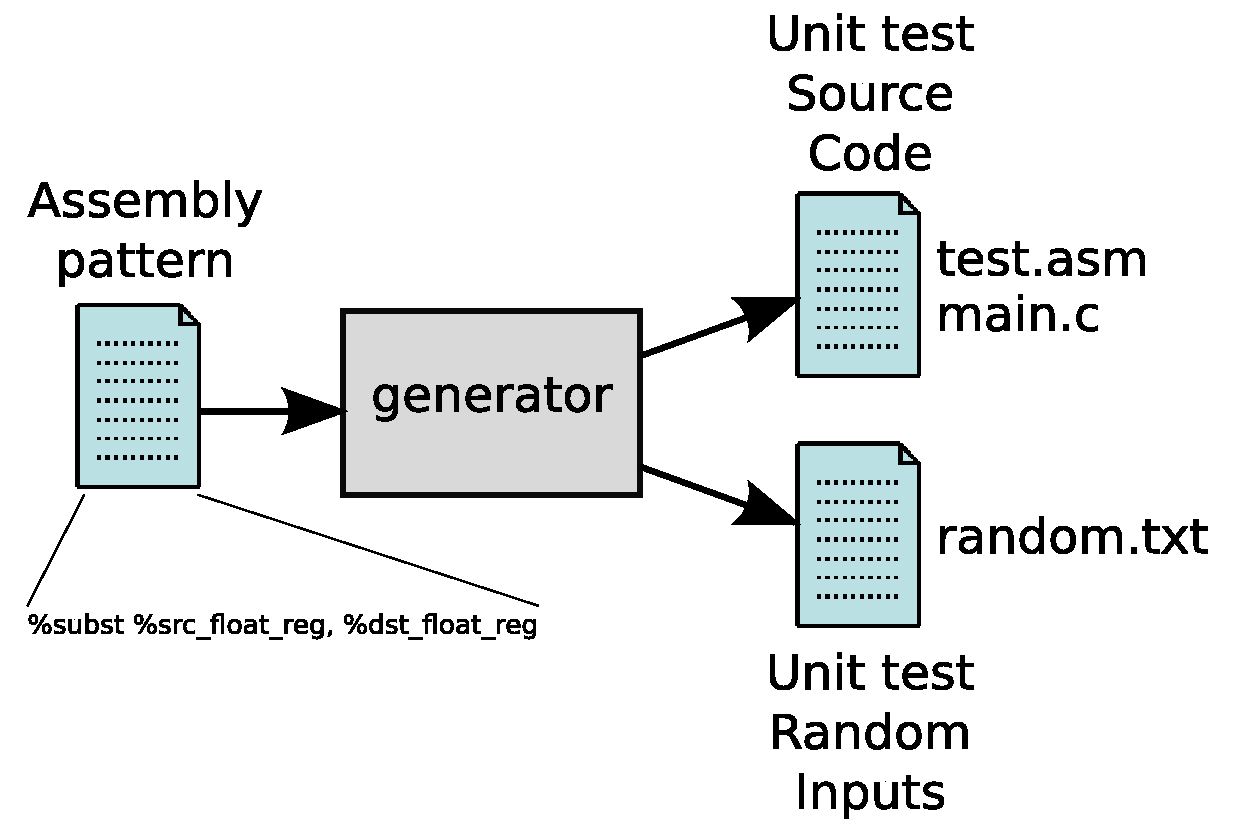
\includegraphics[width=8.0cm]{tms320c3x/fig_unit_test_generator.pdf}
					\caption{\label{fig:tms320c3x_unit_test_generator}UNISIM TMS320C3X unit test generator.}
				\end{center}
			\end{minipage}
			\begin{minipage}{8.0cm}
				\begin{center}
					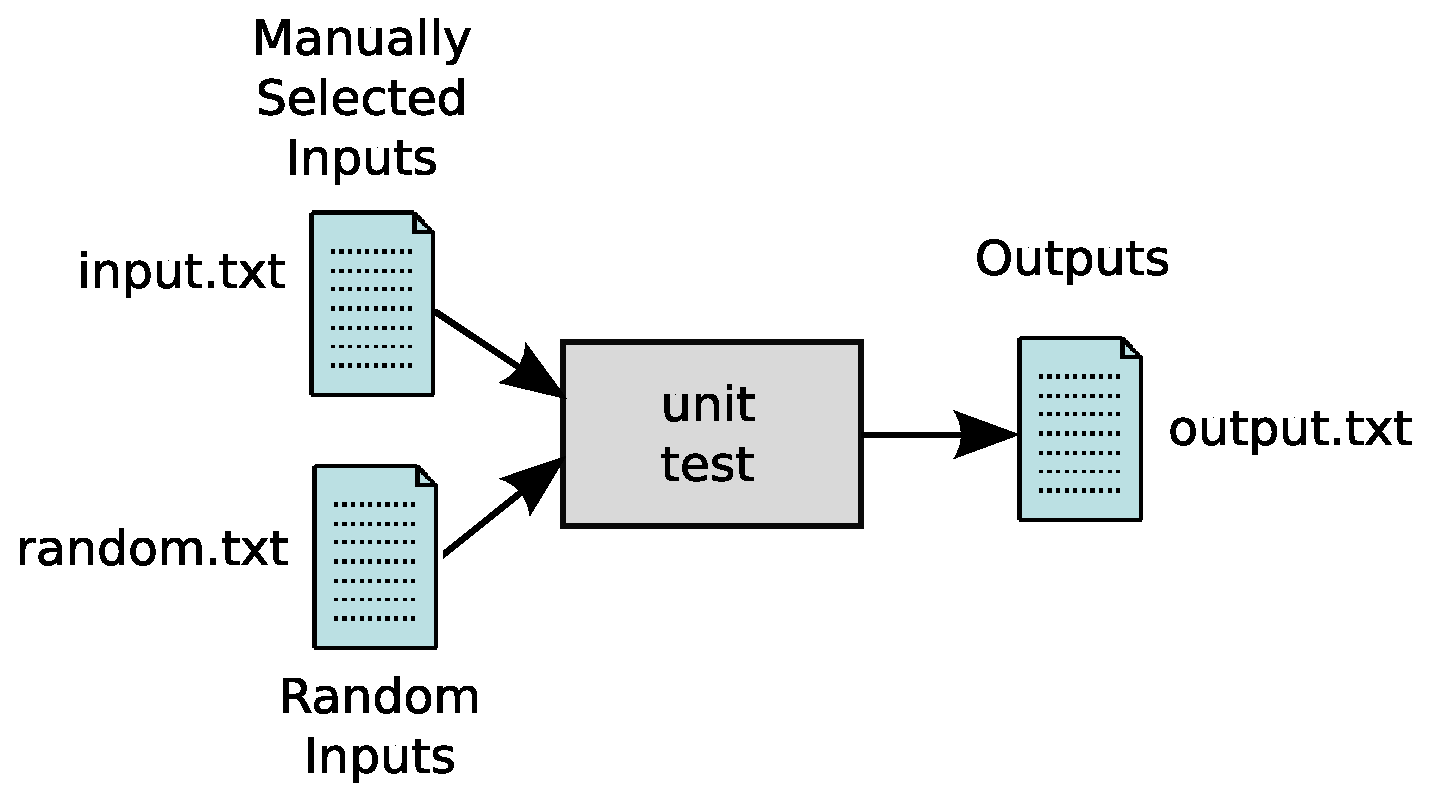
\includegraphics[width=8.0cm]{tms320c3x/fig_unit_test.pdf}
					\caption{\label{fig:tms320c3x_unit_test} A generated unit test.}
				\end{center}
			\end{minipage}
		\end{minipage}
		\vspace{0.5cm}
		\begin{minipage}{\textwidth}
			\begin{center}
				\input{tms320c3x/assembly_pattern}
				\caption{\label{fig:tms320c3x_assembly_pattern} Example of assembly pattern.}
			\end{center}
		\end{minipage}
		\vspace{0.5cm}
		\begin{minipage}{\textwidth}
			\begin{center}
				\tablehead{\hline}
				\tabletail{\hline}
				\begin{supertabular}{|p{16cm}|}
				\multicolumn{1}{|p{16cm}|}{{\scriptsize \texttt{; \it {-}{-}{-}{-}~INPUTS~{-}{-}{-}{-}}\newline
				\texttt{; \it ~r0:~a~32-bit~integer~register}\newline
				\texttt{; \it ~ar2:~an~auxiliary~register~pointing~to~an~array~of~16~32-bit~floating~point~values}\newline
				\texttt{; \it ~r1:~a~32-bit~integer~register~(value~for~st)}\newline
				\texttt{; \it ~r2:~a~40-bit~floating~point~register}\newline
				\texttt{; \it {-}{-}{-}{-}~OUTPUTS~{-}{-}{-}{-}}\newline
				\texttt{; \it ~ar4:~an~auxiliary~register}\newline
				\texttt{; \it ~r2:~a~40-bit~floating~point~register}\newline
				\texttt{; \it ~r3:~a~32-bit~integer~register~(value~of~st)}\newline
				\texttt{~~ldiu~5,~bk~~~~~~~~~~~~~~~~~; \ding{202} \it ~load~block~size~(should~be~at~most~8)}\newline
				\texttt{~~and~5~-~1,~r0~~~~~~~~~~~~~~; \ding{203} \it ~crop~random~value~between~0~and~bk~-~1}\newline
				\texttt{~~ldiu~r0,~ir0~~~~~~~~~~~~~~~; \ding{204} \it ~load~ir0~with~this~random~value}\newline
				\texttt{~~ldiu~ar2,~ar4~~~~~~~~~~~~~~; \ding{205} \it ~load~a~pointer~to~a~buffer~of~16~words}\newline
				\texttt{~~addi~7,~ar4~~~~~~~~~~~~~~~~; \ding{206}}\newline
				\texttt{~~andn~7,~ar4~~~~~~~~~~~~~~~~; \ding{207} \it ~align~circular~buffer~start~on~block~size}\newline
				\texttt{~~ldiu~r1,~st~~~~~~~~~~~~~~~~; \ding{208}}\newline
				\texttt{~~addf~*ar4++(ir0)\%,~r2~~~~~~; \ding{209} \it ~$\leftarrow$~instruction~under~test}\newline
				\texttt{~~ldiu~st,~r3~~~~~~~~~~~~~~~~; \ding{210}}\newline
				\texttt{}}}\\
				\end{supertabular}
				\caption{\label{fig:tms320c3x_generated_assembly} Generated assembly from assembly pattern of Figure~\ref{fig:tms320c3x_assembly_pattern} and substitution strings \texttt{"5"}, \texttt{"7"}, and \texttt{"addf"}.}
			\end{center}
		\end{minipage}
	\end{center}
\end{figure}

The generator needs an assembly pattern and some substitution strings to generate the unit test source code, that is:
\begin{itemize}
\item an assembly function \texttt{unit\_test} (in file \texttt{test.asm}) with the C calling convention and stack parameter passing convention,
\item some random inputs for function \texttt{unit\_test} (\texttt{random.txt}),
\item and a testbench written in C (\texttt{main.c}) that in a loop, reads inputs, calls function \texttt{unit\_test}, and write outputs.
\end{itemize}

An assembly pattern is an assembly source code with special tags. 
These tags start with character \texttt{\%}. 
Most of them represent input/outputs that are substituted by real processor registers during assembly source code generation. 
Tag \texttt{\%subst} is substituted by a substitution string passed as a command line argument to the generator.
Tag \texttt{\%clobber} says to the generator that assembly pattern explicitely clobber register following that tag and that the generator should not allocate that register while substituing inputs and outputs.
Table~\ref{table:tms320c3x_assembly_patterns_tags} lists the available tags.

\begin{table}[p]
\begin{center}
\begin{tabular}{|c|c|l|}
\hline
\textbf{Tag} & \textbf{Type} & \textbf{Storage type}\\
\hline
\texttt{\scriptsize \%src\_int\_reg} & {\scriptsize source} & {\scriptsize 32-bit integer register}\\
\hline
\texttt{\scriptsize \%src\_float\_reg} & {\scriptsize source} & {\scriptsize 40-bit floating-point register}\\
\hline
\texttt{\scriptsize \%src\_aux\_reg} & {\scriptsize source} & {\scriptsize auxiliary register}\\
\hline
\texttt{\scriptsize \%st\_in} & {\scriptsize source} & {\scriptsize 32-bit integer register (value for st)}\\
\hline
\texttt{\scriptsize \%dst\_int\_reg} & {\scriptsize destination} & {\scriptsize 32-bit integer register}\\
\hline
\texttt{\scriptsize \%dst\_float\_reg} & {\scriptsize destination} & {\scriptsize 40-bit floating-point register}\\
\hline
\texttt{\scriptsize \%dst\_aux\_reg} & {\scriptsize destination} & {\scriptsize auxiliary register}\\
\hline
\texttt{\scriptsize \%st\_out} & {\scriptsize destination} & {\scriptsize 32-bit integer register (value of st)}\\
\hline
\texttt{\scriptsize \%src\_dst\_int\_reg} & {\scriptsize source \& destination} & {\scriptsize 32-bit integer register}\\
\hline
\texttt{\scriptsize \%src\_dst\_float\_reg} & {\scriptsize source \& destination} & {\scriptsize 40-bit floating-point register}\\
\hline
\texttt{\scriptsize \%src\_dst\_aux\_reg} & {\scriptsize source \& destination} & {\scriptsize auxiliary register}\\
\hline
\texttt{\scriptsize \%tmp\_int\_reg} & {\scriptsize temporary} & {\scriptsize 32-bit integer register}\\
\hline
\texttt{\scriptsize \%tmp\_float\_reg} & {\scriptsize temporary} & {\scriptsize 40-bit floating-point register}\\
\hline
\texttt{\scriptsize \%tmp\_aux\_reg} & {\scriptsize temporary} & {\scriptsize auxiliary register}\\
\hline
\texttt{\scriptsize \%src\_int\_buf[dim]} & {\scriptsize source} & {\scriptsize auxiliary register pointing to an array of \textit{dim} 32-bit integer values}\\
\hline
\texttt{\scriptsize \%dst\_int\_buf[dim]} & {\scriptsize destination} & {\scriptsize auxiliary register pointing to an array of \textit{dim} 32-bit integer values}\\
\hline
\texttt{\scriptsize \%src\_float\_buf[dim]} & {\scriptsize source} & {\scriptsize auxiliary register pointing to an array of \textit{dim} 32-bit floating-point values}\\
\hline
\texttt{\scriptsize \%dst\_float\_buf[dim]} & {\scriptsize destination} & {\scriptsize auxiliary register pointing to an array of \textit{dim} 32-bit floating-point values}\\
\hline
\texttt{\scriptsize \%subst} & {\scriptsize substitution} & {\scriptsize N/A}\\
\hline
\texttt{\scriptsize \%clobber reg} & {\scriptsize clobber} & {\scriptsize N/A}\\
\hline
\texttt{\scriptsize \%0, \%1, \%2, \ldots} & {\scriptsize reference} & {\scriptsize N/A}\\
\hline
\end{tabular}
\caption{UNISIM TMS320C3X unit test generator assembly patterns tags.}
\label{table:tms320c3x_assembly_patterns_tags}
\end{center}
\end{table}

Figure~\ref{fig:tms320c3x_assembly_pattern} shows an example of assembly pattern and Figure~\ref{fig:tms320c3x_generated_assembly} shows the core of generated assembly. 
During the generation process, each assembly pattern tag is replaced by real processor registers or substitution strings:
\begin{enumerate}
\item[{\large \ding{202}}] \texttt{\%subst} is substituted by integer constant \texttt{5} passed as command line argument of the generator;
\item[{\large \ding{203}}] \texttt{\%0} is substituted as in {\large \ding{202}}, while \texttt{\%src\_int\_reg} is substituted with register \texttt{r0};
\item[{\large \ding{204}}] \texttt{\%clobber ir0} is substituted with register \texttt{ir0} and register \texttt{ir0} is marked as clobbered;
\item[{\large \ding{205}}] \texttt{\%src\_float\_buf[16]} is substituted with register \texttt{ar2} that points to an array of 16 32-bit floating-point values allocated on the stack; \texttt{\%dst\_aux\_reg} is substituted with register \texttt{ar4};
\item[{\large \ding{206}}] \texttt{\%subst} is substituted with integer constant \texttt{7} passed as command line argument to the generator; \texttt{\%6} is substituted as \texttt{\%dst\_aux\_reg} in {\large \ding{205}};
\item[{\large \ding{207}}] \texttt{\%7} is substituted as \texttt{\%subst} in {\large \ding{206}} and \texttt{\%6} is substituted as \texttt{\%dst\_aux\_reg} in {\large \ding{205}};
\item[{\large \ding{208}}] \texttt{\%st\_in} is substituted with register \texttt{r1} and register \texttt{r1} is marked as containing state of register st to enable pretty printing of its content, while \texttt{\%clobber st} is substituted by register \texttt{st} and register \texttt{st} is marked as clobbered;
\item[{\large \ding{209}}] \texttt{\%6} is substituted as \texttt{\%dst\_aux\_reg} in {\large \ding{205}}; \texttt{\%\%} is substituted with \texttt{\%}; \texttt{\%src\_dst\_float\_reg} is substituted with register \texttt{r2};
\item[{\large \ding{210}}] \texttt{\%st\_out} is substituted with register \texttt{r3} and register \texttt{r3} is marked as containing state of register \texttt{st} to enable pretty printing of its content.
\end{enumerate}

The random inputs are obtained with a KISS (Keep It Simple Stupid) random number generator (see \url{http://www.math.niu.edu/\~rusin/known-math/99/RNG}) embedded in the unit tests generator.
The generator creates a uniform distribution for integer numbers. 
Table~\ref{table:tms320c3x_unit_test_float_distribution} shows the distribution for the floating point numbers.

\begin{table}[p]
\begin{center}
\begin{tabular}{|c|c|}
\hline
\textbf{Category} & \textbf{Probability}\\
\hline
-inf & 1/37\\
\hline
smallest negative number & 1/37\\
\hline
zero & 1/37\\
\hline
real zero & 1/37\\
\hline
smallest positive number & 1/37\\
\hline
near to integer & 2/37\\
\hline
+inf & 1/37\\
\hline
small & 2/37\\
\hline
large & 2/37\\ 
\hline
mantissa near previously generated, fully random exponent & 5/37\\
\hline
exponent near previously generated, fully random mantissa & 5/37\\
\hline
float near previously generated & 5/37\\
\hline
fully random & 10/37\\
\hline
\end{tabular}
\caption{UNISIM TMS320C3X unit test generator floating point distribution.}
\label{table:tms320c3x_unit_test_float_distribution}
\end{center}
\end{table}

The unit test source code can be compiled for the development board, and run on both the development board and the UNISIM TMS320C3X simulator.
As a unit test uses the TI C I/O functions, it can reads inputs and write outputs from/to files of the host file system, see Figure~\ref{fig:tms320c3x_unit_test}. 
Such capability has considerably reduced the complexity of testing the assembly pattern under test on both the development board and the UNISIM TMS320C3X simulator.

A unit test reads manually selected inputs from file \texttt{input.txt} and some random generated inputs from file \texttt{random.txt}.
It writes outputs into file \texttt{output.txt}.

\newpage
\subsubsection{The testing environment}
\label{tms320c3x_testing_environment}

A testing environment has been set up using the unit test generator and assembly patterns.
A GNU Makefile is provided to run the unit tests on both the development board (our reference) and the UNISIM TMS320C3X simulator.
The test plan is located in the companion GNU bash script \texttt{factorial.sh}, and more precisely in function '\texttt{factorial}'.
The goal of this function is to generate an auxiliary \texttt{Makefile} (\texttt{Makefile.aux}) that contains building rules of planned unit tests.
A companion C++ program, \texttt{generator} is driven by this auxiliary Makefile to generate the actual unit tests source code.
The generated source code is then compiled for the simulated target using the Texas Instruction cross-compilation tool chain.
The resulting cross-compiled binaries are executed on both a real TMS320C3X DSP using 'Code Composer', and the UNISIM TMS320C3X simulator.
The real/reference execution results and the simulation results are compared, and a failure diagnostic (PASSED or FAILED) is established for each generated unit test program.

As explained in Section~\ref{tms320c3x_unit_tests_generator}, the unit test program output is in file \texttt{output.txt}.
To clearly distinguish simulation results from real execution results, file \texttt{output.txt} (the unit test output) is renamed \texttt{output.ref} when run on the development board or \texttt{output.sim} when run on the UNISIM TMS320C3X simulator.

\noindent The list of supported \texttt{Makefile} targets is the following:

\begin{itemize}
\item \texttt{generator(.exe)}: compile the unit tests generator (\texttt{generator(.exe)})
\item \texttt{compile}: compile the unit tests for the TMS320C3X development board (objects/binaries are \texttt{test.obj}, \texttt{main.obj} and \texttt{test.out})
\item \texttt{rnd}: generate the random input files (\texttt{random.txt}) 
\item \texttt{execute}: execute the unit tests on the TMS320C3X development board (\texttt{EXECUTE} must be set) (execution result is in \texttt{output.ref})
\item \texttt{simulate}: run the simulator (SIMULATE must be set) (simulation results are in \texttt{output.sim})                                    
\item \texttt{check}: compare simulator vs. reference (depends on diff) (check result is in \texttt{output.check})
\item \texttt{diff}: generate difference between simulation vs. reference (depends on \texttt{execute} and \texttt{simulate}) (diff result is in \texttt{output.diff})
\item \texttt{regression-test}: launch a regression test of the UNISIM TMS320C3X simulator
\item \texttt{doc}: generate unit tests documentation (\texttt{unit\_tests.pdf})
\item \texttt{dist}: distribute the testing environment together with reference outputs (\texttt{output.ref})
\item \texttt{clean}: clean everything (but execution results, use \texttt{cleanref} for that)
\item \texttt{cleangen}: clean generator executable (\texttt{generator(.exe)})
\item \texttt{cleansrc}: clean TMS320C3X generated source files (\texttt{test.asm} and \texttt{main.c})
\item \texttt{cleanrnd}: clean generated random input files (\texttt{random.txt})
\item \texttt{cleanbin}: clean TMS320C3X executable files (\texttt{test.out})
\item \texttt{cleanobj}: clean TMS320C3X object files (\texttt{test.obj} and \texttt{main.obj})
\item \texttt{cleangel}: clean GEL scripts (\texttt{run.gel})
\item \texttt{cleansim}: clean simulation results (\texttt{output.sim})
\item \texttt{cleanref}: clean execution results (\texttt{output.ref})
\item \texttt{cleandiff}: clean diff files (\texttt{output.diff})
\item \texttt{cleancheck}: clean check files (\texttt{output.check})
\item \texttt{cleandoc}: clean latex files (\texttt{test.tex})
\end{itemize}

\noindent The following \texttt{Makefile} variables are available for tuning the \texttt{Makefile}:
\begin{itemize}
\item Mandatory:
	\begin{itemize}
	\item \texttt{SIMULATE}: path to the UNISIM TMS320C3X simulator binary
	\item \texttt{EXECUTE}: path to Code Composer executable (i.e. \texttt{cc\_app.exe})
	\item \texttt{DIST\_DIR}: path to destination directory for a distribution
	\end{itemize}
\item Optional:
	\begin{itemize}
	\item \texttt{COMPILER\_PREFIX}: prefix to add before the compiler tools executables names (default: empty)
	\end{itemize}
\end{itemize}

The provided \texttt{Makefile} uses a GNU bash script \texttt{factorial.sh}, that contains a factorial plan, to generate most of the \texttt{Makefile} rules in file \texttt{Makefile.aux}.
To obtain the reference outputs from the developement board, do the following at the command prompt:
\begin{verbatim}
$ make execute EXECUTE=cc_app.exe
\end{verbatim}

Figure~\ref{fig:tms320c3x_cc} shows the testing environment running on Windows and launching unit tests on the development board.

\begin{figure}[!h]
	\begin{center}
		\begin{minipage}{\textwidth}
			\begin{minipage}{9.5cm}
				\begin{center}
					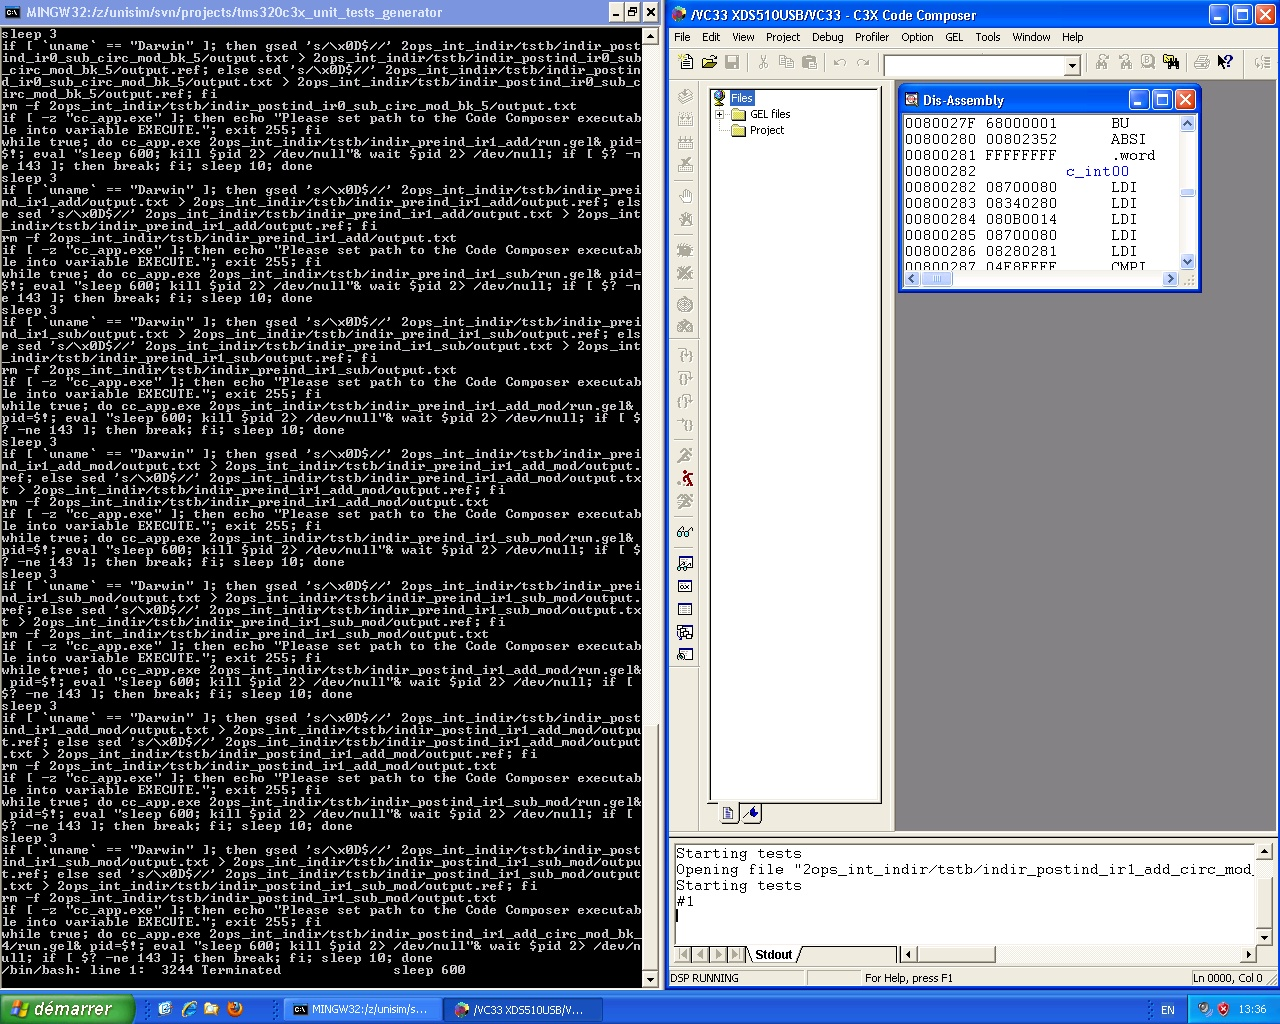
\includegraphics[width=9.0cm]{tms320c3x/fig_code_composer.jpg}
					\caption{\label{fig:tms320c3x_cc} GNU Make (on the left) launching unit tests on the development board using code composer (on the right)}
				\end{center}
			\end{minipage}
			\begin{minipage}{6.5cm}
				\begin{center}
		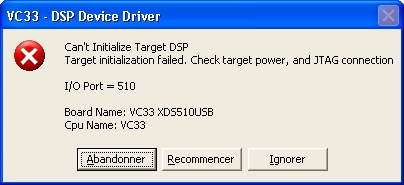
\includegraphics[width=6.0cm]{tms320c3x/fig_driver_error.jpg}
		\caption{\label{fig:tms320c3x_driver_error} VC33 device driver communication problem.}
				\end{center}
			\end{minipage}
		\end{minipage}
	\end{center}
\end{figure}

\textit{Note: You may experience frequent failures of the JTAG Emulator (red LED that indicates activity over USB get stuck), making Code Composer complain in a dialog box that it can't initialize target DSP, see Figure~\ref{fig:tms320c3x_driver_error}. Disconnect and reconnect the USB cable on the JTAG emulator, and then click button "Retry" to resume execution.}

\vspace{0.5cm}

To obtain the simulation outputs from the UNISIM TMS320C3X simulator, do the following at the command prompt:
\begin{verbatim}
$ make simulate SIMULATE=path-to-unisim-tms320c3x-2.0
\end{verbatim}

\subsubsection{Regression tests}
\label{tms320c3x_regression_tests}

The testing environment also acts as a regression test for UNISIM TMS320C3X simulator as the expected results (\texttt{output.ref}) are already provided in the testing environment.

To cross-compile the unit tests programs, do the following at the command prompt on the cross-compilation host:
\begin{verbatim}
$ make generator
$ make compile
$ make c31boot.out
\end{verbatim}

Then to check that all unit tests successfully run on the UNISIM TMS320C3X simulator, do the following at the command prompt on the simulation host:
\begin{verbatim}
$ make cleangen
$ make generator
$ make regression-test SIMULATE=path-to-unisim-tms320c3x-2.0
\end{verbatim}

\noindent The result for each unit test program is either \texttt{PASSED} or \texttt{FAILED}.\\

\textit{Note: At most one instance of the Texas Instrument Cross-compiler can be run at a time (at least on a Windows host and Wine).
Using \texttt{flag -j} of GNU Make when compiling the unit tests programs results in unexpected behaviors.}

\textit{Note: Unit test program \texttt{parallel\_float/stf\_stf/reg\_buf} will likely fail because of a bug in instruction \texttt{STF || STF} in the TMS320VC33 of our development board.}


\newpage
\appendix
\appendixpage
\section{Simulator technical reference (generated)}
\label{techref}
This documentation has been automatically generated from the simulator \texttt{UNISIM tms320c3x} version 2.0 on Oct 18 2013.
\subsection{Introduction}
UNISIM tms320c3x, a TMS320C3X DSP simulator with support of TI COFF binaries, and TI C I/O (RTS run-time).\\
Section \ref{UNISIM tms320c3x_licensing} gives licensing informations about the simulator.
Section \ref{UNISIM tms320c3x_simulated_configuration} shows the set of modules and services that compose the simulator.
Section \ref{UNISIM tms320c3x_using} shows how to invoke the simulator at the command line prompt.
Section \ref{UNISIM tms320c3x_configuration} gives the simulator parameters.
Section \ref{UNISIM tms320c3x_statistics} gives the simulator statistic counters.
Section \ref{UNISIM tms320c3x_formulas} gives the simulator statistic formulas.
\subsection{Licensing}
\label{UNISIM tms320c3x_licensing}
UNISIM tms320c3x 2.0\\
Copyright (C) 2009-2013, Commissariat a l'Energie Atomique (CEA)\\
License: BSD (see file COPYING)\\
Authors: Gilles Mouchard $<$gilles.mouchard@cea.fr$>$, Daniel Gracia P\'erez $<$daniel.gracia-perez@cea.fr$>$\\
\subsection{Simulated configuration}
\label{UNISIM tms320c3x_simulated_configuration}
\noindent The UNISIM tms320c3x simulator is composed of the following modules and services:
\begin{itemize}\addtolength{\itemsep}{-0.40\baselineskip}
\item \textbf{cpu}: this module implements a TMS320C3X DSP core
\item \textbf{debugger}
\item \textbf{dint-stub}: An initiator stub
\item \textbf{gdb-server}: this service implements the GDB server remote serial protocol over TCP/IP. Standards GDB clients (e.g. gdb, eclipse, ddd) can connect to the simulator to debug the target application that runs within the simulator.
\item \textbf{host-time}: this service is an abstraction layer for the host machine time
\item \textbf{inline-debugger}: this service implements a built-in debugger in the terminal console
\item \textbf{int0-stub}: An initiator stub
\item \textbf{int1-stub}: An initiator stub
\item \textbf{int2-stub}: An initiator stub
\item \textbf{int3-stub}: An initiator stub
\item \textbf{loader}: A multi-format loader that supports ELF32, ELF64, S19, COFF and Raw binary files
\item \textbf{loader.file0}
\item \textbf{loader.memory-mapper}: A memory mapper
\item \textbf{loader.tee-backtrace}: This service/client implements a tee ('T'). It unifies the backtrace capability of several services that individually provides their own backtrace capability
\item \textbf{loader.tee-blob}: This service/client implements a tee ('T'). It unifies the statement lookup capability of several services that individually provides their own statement lookup capability
\item \textbf{loader.tee-loader}: This service/client implements a tee ('T'). It unifies the loader capability of several services that individually provides their own loader capability
\item \textbf{loader.tee-stmt-lookup}: This service/client implements a tee ('T'). It unifies the statement lookup capability of several services that individually provides their own statement lookup capability
\item \textbf{loader.tee-symbol-table-lookup}: This service/client implements a tee ('T'). It unifies the symbol table lookup capability of several services that individually provides their own symbol table lookup capability
\item \textbf{memory}: this module implements a memory
\item \textbf{profiler}
\item \textbf{rint0-stub}: An initiator stub
\item \textbf{rint1-stub}: An initiator stub
\item \textbf{tee-memory-access-reporting}
\item \textbf{tee-memory-access-reporting.tee-memory-access-reporting.control\_selector[0]}
\item \textbf{tee-memory-access-reporting.tee-memory-access-reporting.control\_selector[10]}
\item \textbf{tee-memory-access-reporting.tee-memory-access-reporting.control\_selector[11]}
\item \textbf{tee-memory-access-reporting.tee-memory-access-reporting.control\_selector[12]}
\item \textbf{tee-memory-access-reporting.tee-memory-access-reporting.control\_selector[13]}
\item \textbf{tee-memory-access-reporting.tee-memory-access-reporting.control\_selector[14]}
\item \textbf{tee-memory-access-reporting.tee-memory-access-reporting.control\_selector[15]}
\item \textbf{tee-memory-access-reporting.tee-memory-access-reporting.control\_selector[1]}
\item \textbf{tee-memory-access-reporting.tee-memory-access-reporting.control\_selector[2]}
\item \textbf{tee-memory-access-reporting.tee-memory-access-reporting.control\_selector[3]}
\item \textbf{tee-memory-access-reporting.tee-memory-access-reporting.control\_selector[4]}
\item \textbf{tee-memory-access-reporting.tee-memory-access-reporting.control\_selector[5]}
\item \textbf{tee-memory-access-reporting.tee-memory-access-reporting.control\_selector[6]}
\item \textbf{tee-memory-access-reporting.tee-memory-access-reporting.control\_selector[7]}
\item \textbf{tee-memory-access-reporting.tee-memory-access-reporting.control\_selector[8]}
\item \textbf{tee-memory-access-reporting.tee-memory-access-reporting.control\_selector[9]}
\item \textbf{ti-c-io}
\item \textbf{time}: this service is an abstraction layer for the SystemC kernel time
\item \textbf{tint0-stub}: An initiator stub
\item \textbf{tint1-stub}: An initiator stub
\item \textbf{xint0-stub}: An initiator stub
\item \textbf{xint1-stub}: An initiator stub
\end{itemize}
\subsection{Using the UNISIM tms320c3x simulator}
\label{UNISIM tms320c3x_using}
The UNISIM tms320c3x simulator has the following command line options:\\
~\\
\noindent Usage: \texttt{unisim-tms320c3x-2.0 [<options>] [...]}

\noindent Options:
\begin{itemize}
\item \texttt{--set $<$param=value$>$ or -s $<$param=value$>$}: set value of parameter 'param' to 'value'
\item \texttt{--config $<$XML file$>$ or -c $<$XML file$>$}: configures the simulator with the given XML configuration file
\item \texttt{--get-config $<$XML file$>$ or -g $<$XML file$>$}: get the simulator configuration XML file (you can use it to create your own configuration. This option can be combined with -c to get a new configuration file with existing variables from another file
\item \texttt{--list or -l}: lists all available parameters, their type, and their current value
\item \texttt{--warn or -w}: enable printing of kernel warnings
\item \texttt{--doc $<$Latex file$>$ or -d $<$Latex file$>$}: enable printing a latex documentation
\item \texttt{--version or -v}: displays the program version information
\item \texttt{--share-path $<$path$>$ or -p $<$path$>$}: the path that should be used for the share directory (absolute path)
\item \texttt{--help or -h}: displays this help
\end{itemize}
\subsection{Configuration}
\label{UNISIM tms320c3x_configuration}
Simulator configuration (see below) can be modified using command line Options \texttt{--set $<$param=value$>$} or \texttt{--config $<$config file$>$}.\\
~\\
\tablehead{\hline}
\tabletail{\hline}
\begin{supertabular}{|p{7.5cm}|p{7.5cm}|}
\multicolumn{2}{|l|}{\textbf{\Large Global}}\\
\hline
\multicolumn{1}{|p{7.5cm}}{\textbf{Name:} \texttt{enable-gdb-server}} & \multicolumn{1}{p{7.5cm}|}{\textbf{Type:} \texttt{parameter}}\\
\multicolumn{1}{|p{7.5cm}}{\textbf{Default:} \texttt{true}} & \multicolumn{1}{p{7.5cm}|}{\textbf{Data type:} \texttt{boolean}}\\
\multicolumn{2}{|p{15cm}|}{\textbf{Valid:} \texttt{true},~\texttt{false}}\\
\multicolumn{2}{|l|}{}\\
\multicolumn{2}{|p{15cm}|}{\textbf{Description:} \newline Enable/Disable GDB server instantiation.}\\
\hline
\multicolumn{1}{|p{7.5cm}}{\textbf{Name:} \texttt{enable-inline-debugger}} & \multicolumn{1}{p{7.5cm}|}{\textbf{Type:} \texttt{parameter}}\\
\multicolumn{1}{|p{7.5cm}}{\textbf{Default:} \texttt{true}} & \multicolumn{1}{p{7.5cm}|}{\textbf{Data type:} \texttt{boolean}}\\
\multicolumn{2}{|p{15cm}|}{\textbf{Valid:} \texttt{true},~\texttt{false}}\\
\multicolumn{2}{|l|}{}\\
\multicolumn{2}{|p{15cm}|}{\textbf{Description:} \newline Enable/Disable inline debugger instantiation.}\\
\hline
\multicolumn{1}{|p{7.5cm}}{\textbf{Name:} \texttt{enable-press-enter-at-exit}} & \multicolumn{1}{p{7.5cm}|}{\textbf{Type:} \texttt{parameter}}\\
\multicolumn{1}{|p{7.5cm}}{\textbf{Default:} \texttt{false}} & \multicolumn{1}{p{7.5cm}|}{\textbf{Data type:} \texttt{boolean}}\\
\multicolumn{2}{|p{15cm}|}{\textbf{Valid:} \texttt{true},~\texttt{false}}\\
\multicolumn{2}{|l|}{}\\
\multicolumn{2}{|p{15cm}|}{\textbf{Description:} \newline Enable/Disable pressing key enter at exit.}\\
\hline
\multicolumn{1}{|p{7.5cm}}{\textbf{Name:} \texttt{kernel\_logger.file}} & \multicolumn{1}{p{7.5cm}|}{\textbf{Type:} \texttt{parameter}}\\
\multicolumn{1}{|p{7.5cm}}{\textbf{Default:} \texttt{false}} & \multicolumn{1}{p{7.5cm}|}{\textbf{Data type:} \texttt{boolean}}\\
\multicolumn{2}{|p{15cm}|}{\textbf{Valid:} \texttt{true},~\texttt{false}}\\
\multicolumn{2}{|l|}{}\\
\multicolumn{2}{|p{15cm}|}{\textbf{Description:} \newline Keep logger output in a file.}\\
\hline
\multicolumn{1}{|p{7.5cm}}{\textbf{Name:} \texttt{kernel\_logger.filename}} & \multicolumn{1}{p{7.5cm}|}{\textbf{Type:} \texttt{parameter}}\\
\multicolumn{1}{|p{7.5cm}}{\textbf{Default:} \texttt{logger\_output.txt}} & \multicolumn{1}{p{7.5cm}|}{\textbf{Data type:} \texttt{string}}\\
\multicolumn{2}{|l|}{}\\
\multicolumn{2}{|l|}{}\\
\multicolumn{2}{|p{15cm}|}{\textbf{Description:} \newline Filename to keep logger output \_(the option file must be activated).}\\
\hline
\multicolumn{1}{|p{7.5cm}}{\textbf{Name:} \texttt{kernel\_logger.std\_err}} & \multicolumn{1}{p{7.5cm}|}{\textbf{Type:} \texttt{parameter}}\\
\multicolumn{1}{|p{7.5cm}}{\textbf{Default:} \texttt{true}} & \multicolumn{1}{p{7.5cm}|}{\textbf{Data type:} \texttt{boolean}}\\
\multicolumn{2}{|p{15cm}|}{\textbf{Valid:} \texttt{true},~\texttt{false}}\\
\multicolumn{2}{|l|}{}\\
\multicolumn{2}{|p{15cm}|}{\textbf{Description:} \newline Show logger output through the standard error output.}\\
\hline
\multicolumn{1}{|p{7.5cm}}{\textbf{Name:} \texttt{kernel\_logger.std\_err\_color}} & \multicolumn{1}{p{7.5cm}|}{\textbf{Type:} \texttt{parameter}}\\
\multicolumn{1}{|p{7.5cm}}{\textbf{Default:} \texttt{false}} & \multicolumn{1}{p{7.5cm}|}{\textbf{Data type:} \texttt{boolean}}\\
\multicolumn{2}{|p{15cm}|}{\textbf{Valid:} \texttt{true},~\texttt{false}}\\
\multicolumn{2}{|l|}{}\\
\multicolumn{2}{|p{15cm}|}{\textbf{Description:} \newline Colorize logger output through the standard error output \_(only works if std\_err is active).}\\
\hline
\multicolumn{1}{|p{7.5cm}}{\textbf{Name:} \texttt{kernel\_logger.std\_out}} & \multicolumn{1}{p{7.5cm}|}{\textbf{Type:} \texttt{parameter}}\\
\multicolumn{1}{|p{7.5cm}}{\textbf{Default:} \texttt{false}} & \multicolumn{1}{p{7.5cm}|}{\textbf{Data type:} \texttt{boolean}}\\
\multicolumn{2}{|p{15cm}|}{\textbf{Valid:} \texttt{true},~\texttt{false}}\\
\multicolumn{2}{|l|}{}\\
\multicolumn{2}{|p{15cm}|}{\textbf{Description:} \newline Show logger output through the standard output.}\\
\hline
\multicolumn{1}{|p{7.5cm}}{\textbf{Name:} \texttt{kernel\_logger.std\_out\_color}} & \multicolumn{1}{p{7.5cm}|}{\textbf{Type:} \texttt{parameter}}\\
\multicolumn{1}{|p{7.5cm}}{\textbf{Default:} \texttt{false}} & \multicolumn{1}{p{7.5cm}|}{\textbf{Data type:} \texttt{boolean}}\\
\multicolumn{2}{|p{15cm}|}{\textbf{Valid:} \texttt{true},~\texttt{false}}\\
\multicolumn{2}{|l|}{}\\
\multicolumn{2}{|p{15cm}|}{\textbf{Description:} \newline Colorize logger output through the standard output \_(only works if std\_out is active).}\\
\hline
\multicolumn{1}{|p{7.5cm}}{\textbf{Name:} \texttt{kernel\_logger.xml\_file}} & \multicolumn{1}{p{7.5cm}|}{\textbf{Type:} \texttt{parameter}}\\
\multicolumn{1}{|p{7.5cm}}{\textbf{Default:} \texttt{false}} & \multicolumn{1}{p{7.5cm}|}{\textbf{Data type:} \texttt{boolean}}\\
\multicolumn{2}{|p{15cm}|}{\textbf{Valid:} \texttt{true},~\texttt{false}}\\
\multicolumn{2}{|l|}{}\\
\multicolumn{2}{|p{15cm}|}{\textbf{Description:} \newline Keep logger output in a file xml formatted.}\\
\hline
\multicolumn{1}{|p{7.5cm}}{\textbf{Name:} \texttt{kernel\_logger.xml\_file\_gzipped}} & \multicolumn{1}{p{7.5cm}|}{\textbf{Type:} \texttt{parameter}}\\
\multicolumn{1}{|p{7.5cm}}{\textbf{Default:} \texttt{false}} & \multicolumn{1}{p{7.5cm}|}{\textbf{Data type:} \texttt{boolean}}\\
\multicolumn{2}{|p{15cm}|}{\textbf{Valid:} \texttt{true},~\texttt{false}}\\
\multicolumn{2}{|l|}{}\\
\multicolumn{2}{|p{15cm}|}{\textbf{Description:} \newline If the xml\_file option is active, the output file will be compressed (a .gz extension will be automatically added to the xml\_filename option.}\\
\hline
\multicolumn{1}{|p{7.5cm}}{\textbf{Name:} \texttt{kernel\_logger.xml\_filename}} & \multicolumn{1}{p{7.5cm}|}{\textbf{Type:} \texttt{parameter}}\\
\multicolumn{1}{|p{7.5cm}}{\textbf{Default:} \texttt{logger\_output.xml}} & \multicolumn{1}{p{7.5cm}|}{\textbf{Data type:} \texttt{string}}\\
\multicolumn{2}{|l|}{}\\
\multicolumn{2}{|l|}{}\\
\multicolumn{2}{|p{15cm}|}{\textbf{Description:} \newline Filename to keep logger xml output \_(the option xml\_file must be activated).}\\
\hline
\hline
\multicolumn{2}{|l|}{\textbf{\Large cpu}}\\
\hline
\multicolumn{1}{|p{7.5cm}}{\textbf{Name:} \texttt{cpu.max-inst}} & \multicolumn{1}{p{7.5cm}|}{\textbf{Type:} \texttt{parameter}}\\
\multicolumn{1}{|p{7.5cm}}{\textbf{Default:} \texttt{0xffffffffffffffff}} & \multicolumn{1}{p{7.5cm}|}{\textbf{Data type:} \texttt{unsigned 64-bit integer}}\\
\multicolumn{2}{|l|}{}\\
\hline
\multicolumn{1}{|p{7.5cm}}{\textbf{Name:} \texttt{cpu.trap-on-instruction-counter}} & \multicolumn{1}{p{7.5cm}|}{\textbf{Type:} \texttt{parameter}}\\
\multicolumn{1}{|p{7.5cm}}{\textbf{Default:} \texttt{0xffffffffffffffff}} & \multicolumn{1}{p{7.5cm}|}{\textbf{Data type:} \texttt{unsigned 64-bit integer}}\\
\multicolumn{2}{|l|}{}\\
\hline
\multicolumn{1}{|p{7.5cm}}{\textbf{Name:} \texttt{cpu.mimic-dev-board}} & \multicolumn{1}{p{7.5cm}|}{\textbf{Type:} \texttt{parameter}}\\
\multicolumn{1}{|p{7.5cm}}{\textbf{Default:} \texttt{true}} & \multicolumn{1}{p{7.5cm}|}{\textbf{Data type:} \texttt{boolean}}\\
\multicolumn{2}{|p{15cm}|}{\textbf{Valid:} \texttt{true},~\texttt{false}}\\
\hline
\multicolumn{1}{|p{7.5cm}}{\textbf{Name:} \texttt{cpu.trap-on-trap-instruction}} & \multicolumn{1}{p{7.5cm}|}{\textbf{Type:} \texttt{parameter}}\\
\multicolumn{1}{|p{7.5cm}}{\textbf{Default:} \texttt{0x7400003f}} & \multicolumn{1}{p{7.5cm}|}{\textbf{Data type:} \texttt{unsigned 32-bit integer}}\\
\multicolumn{2}{|l|}{}\\
\multicolumn{2}{|l|}{}\\
\multicolumn{2}{|p{15cm}|}{\textbf{Description:} \newline if not zero, encoding of trap instruction that should trap into debugger.}\\
\hline
\multicolumn{1}{|p{7.5cm}}{\textbf{Name:} \texttt{cpu.enable-parallel-load-bug}} & \multicolumn{1}{p{7.5cm}|}{\textbf{Type:} \texttt{parameter}}\\
\multicolumn{1}{|p{7.5cm}}{\textbf{Default:} \texttt{true}} & \multicolumn{1}{p{7.5cm}|}{\textbf{Data type:} \texttt{boolean}}\\
\multicolumn{2}{|p{15cm}|}{\textbf{Valid:} \texttt{true},~\texttt{false}}\\
\multicolumn{2}{|l|}{}\\
\multicolumn{2}{|p{15cm}|}{\textbf{Description:} \newline When using parallel loads (LDF src2, dst2 || LDF src1, dst1) the src1 load doesn't transform incorrect zero values to valid zero representation, instead they copy the contents of the memory to the register. Set to this parameter to false to transform incorrect zero values..}\\
\hline
\multicolumn{1}{|p{7.5cm}}{\textbf{Name:} \texttt{cpu.enable-rnd-bug}} & \multicolumn{1}{p{7.5cm}|}{\textbf{Type:} \texttt{parameter}}\\
\multicolumn{1}{|p{7.5cm}}{\textbf{Default:} \texttt{true}} & \multicolumn{1}{p{7.5cm}|}{\textbf{Data type:} \texttt{boolean}}\\
\multicolumn{2}{|p{15cm}|}{\textbf{Valid:} \texttt{true},~\texttt{false}}\\
\multicolumn{2}{|l|}{}\\
\multicolumn{2}{|p{15cm}|}{\textbf{Description:} \newline If enabled the `rnd` instruction sets the Z flag to 0 systematically, as it is done in the evaluation board. Otherwise, Z is unchanged as it is written in the documentation..}\\
\hline
\multicolumn{1}{|p{7.5cm}}{\textbf{Name:} \texttt{cpu.enable-parallel-store-} \newline$\hookrightarrow$\texttt{bug}} & \multicolumn{1}{p{7.5cm}|}{\textbf{Type:} \texttt{parameter}}\\
\multicolumn{1}{|p{7.5cm}}{\textbf{Default:} \texttt{true}} & \multicolumn{1}{p{7.5cm}|}{\textbf{Data type:} \texttt{boolean}}\\
\multicolumn{2}{|p{15cm}|}{\textbf{Valid:} \texttt{true},~\texttt{false}}\\
\multicolumn{2}{|l|}{}\\
\multicolumn{2}{|p{15cm}|}{\textbf{Description:} \newline If enabled, when using parallel stores (STF src2, dst2 || STF src1, dst1) the first store is treated as a NOP..}\\
\hline
\multicolumn{1}{|p{7.5cm}}{\textbf{Name:} \texttt{cpu.enable-float-ops-with-} \newline$\hookrightarrow$\texttt{non-ext-regs}} & \multicolumn{1}{p{7.5cm}|}{\textbf{Type:} \texttt{parameter}}\\
\multicolumn{1}{|p{7.5cm}}{\textbf{Default:} \texttt{false}} & \multicolumn{1}{p{7.5cm}|}{\textbf{Data type:} \texttt{boolean}}\\
\multicolumn{2}{|p{15cm}|}{\textbf{Valid:} \texttt{true},~\texttt{false}}\\
\multicolumn{2}{|l|}{}\\
\multicolumn{2}{|p{15cm}|}{\textbf{Description:} \newline If enabled non extended registers can be used on all the float instructions, however the behavior is not documented and can differ between chips revision. If disabled, it stops simulation when using non extended registers on float instructions..}\\
\hline
\multicolumn{1}{|p{7.5cm}}{\textbf{Name:} \texttt{cpu.verbose-all}} & \multicolumn{1}{p{7.5cm}|}{\textbf{Type:} \texttt{parameter}}\\
\multicolumn{1}{|p{7.5cm}}{\textbf{Default:} \texttt{false}} & \multicolumn{1}{p{7.5cm}|}{\textbf{Data type:} \texttt{boolean}}\\
\multicolumn{2}{|p{15cm}|}{\textbf{Valid:} \texttt{true},~\texttt{false}}\\
\hline
\multicolumn{1}{|p{7.5cm}}{\textbf{Name:} \texttt{cpu.verbose-setup}} & \multicolumn{1}{p{7.5cm}|}{\textbf{Type:} \texttt{parameter}}\\
\multicolumn{1}{|p{7.5cm}}{\textbf{Default:} \texttt{false}} & \multicolumn{1}{p{7.5cm}|}{\textbf{Data type:} \texttt{boolean}}\\
\multicolumn{2}{|p{15cm}|}{\textbf{Valid:} \texttt{true},~\texttt{false}}\\
\hline
\multicolumn{1}{|p{7.5cm}}{\textbf{Name:} \texttt{cpu.cpu-cycle-time}} & \multicolumn{1}{p{7.5cm}|}{\textbf{Type:} \texttt{parameter}}\\
\multicolumn{1}{|p{7.5cm}}{\textbf{Default:} \texttt{13333 ps}} & \multicolumn{1}{p{7.5cm}|}{\textbf{Data type:} \texttt{sc\_time}}\\
\multicolumn{2}{|l|}{}\\
\multicolumn{2}{|l|}{}\\
\multicolumn{2}{|p{15cm}|}{\textbf{Description:} \newline cpu cycle time.}\\
\hline
\multicolumn{1}{|p{7.5cm}}{\textbf{Name:} \texttt{cpu.nice-time}} & \multicolumn{1}{p{7.5cm}|}{\textbf{Type:} \texttt{parameter}}\\
\multicolumn{1}{|p{7.5cm}}{\textbf{Default:} \texttt{1 us}} & \multicolumn{1}{p{7.5cm}|}{\textbf{Data type:} \texttt{sc\_time}}\\
\multicolumn{2}{|l|}{}\\
\multicolumn{2}{|l|}{}\\
\multicolumn{2}{|p{15cm}|}{\textbf{Description:} \newline maximum time between synchonizations.}\\
\hline
\multicolumn{1}{|p{7.5cm}}{\textbf{Name:} \texttt{cpu.ipc}} & \multicolumn{1}{p{7.5cm}|}{\textbf{Type:} \texttt{parameter}}\\
\multicolumn{1}{|p{7.5cm}}{\textbf{Default:} \texttt{1}} & \multicolumn{1}{p{7.5cm}|}{\textbf{Data type:} \texttt{double precision floating-point}}\\
\multicolumn{2}{|l|}{}\\
\multicolumn{2}{|l|}{}\\
\multicolumn{2}{|p{15cm}|}{\textbf{Description:} \newline targeted average instructions per second.}\\
\hline
\multicolumn{1}{|p{7.5cm}}{\textbf{Name:} \texttt{cpu.enable-dmi}} & \multicolumn{1}{p{7.5cm}|}{\textbf{Type:} \texttt{parameter}}\\
\multicolumn{1}{|p{7.5cm}}{\textbf{Default:} \texttt{true}} & \multicolumn{1}{p{7.5cm}|}{\textbf{Data type:} \texttt{boolean}}\\
\multicolumn{2}{|p{15cm}|}{\textbf{Valid:} \texttt{true},~\texttt{false}}\\
\multicolumn{2}{|l|}{}\\
\multicolumn{2}{|p{15cm}|}{\textbf{Description:} \newline Enable/Disable TLM 2.0 DMI (Direct Memory Access) to speed-up simulation.}\\
\hline
\multicolumn{1}{|p{7.5cm}}{\textbf{Name:} \texttt{cpu.debug-dmi}} & \multicolumn{1}{p{7.5cm}|}{\textbf{Type:} \texttt{parameter}}\\
\multicolumn{1}{|p{7.5cm}}{\textbf{Default:} \texttt{false}} & \multicolumn{1}{p{7.5cm}|}{\textbf{Data type:} \texttt{boolean}}\\
\multicolumn{2}{|p{15cm}|}{\textbf{Valid:} \texttt{true},~\texttt{false}}\\
\multicolumn{2}{|l|}{}\\
\multicolumn{2}{|p{15cm}|}{\textbf{Description:} \newline Enable/Disable debugging of DMI (Direct Memory Access).}\\
\hline
\hline
\multicolumn{2}{|l|}{\textbf{\Large debugger}}\\
\hline
\multicolumn{1}{|p{7.5cm}}{\textbf{Name:} \texttt{debugger.verbose}} & \multicolumn{1}{p{7.5cm}|}{\textbf{Type:} \texttt{parameter}}\\
\multicolumn{1}{|p{7.5cm}}{\textbf{Default:} \texttt{false}} & \multicolumn{1}{p{7.5cm}|}{\textbf{Data type:} \texttt{boolean}}\\
\multicolumn{2}{|p{15cm}|}{\textbf{Valid:} \texttt{true},~\texttt{false}}\\
\multicolumn{2}{|l|}{}\\
\multicolumn{2}{|p{15cm}|}{\textbf{Description:} \newline Enable/Disable verbosity.}\\
\hline
\multicolumn{1}{|p{7.5cm}}{\textbf{Name:} \texttt{debugger.dwarf-to-html-output-} \newline$\hookrightarrow$\texttt{directory}} & \multicolumn{1}{p{7.5cm}|}{\textbf{Type:} \texttt{parameter}}\\
\multicolumn{1}{|p{7.5cm}}{\textbf{Default:} \texttt{}} & \multicolumn{1}{p{7.5cm}|}{\textbf{Data type:} \texttt{string}}\\
\multicolumn{2}{|l|}{}\\
\multicolumn{2}{|l|}{}\\
\multicolumn{2}{|p{15cm}|}{\textbf{Description:} \newline DWARF v2/v3 to HTML output directory.}\\
\hline
\multicolumn{1}{|p{7.5cm}}{\textbf{Name:} \texttt{debugger.dwarf-register-number-} \newline$\hookrightarrow$\texttt{mapping-filename}} & \multicolumn{1}{p{7.5cm}|}{\textbf{Type:} \texttt{parameter}}\\
\multicolumn{1}{|p{7.5cm}}{\textbf{Default:} \texttt{}} & \multicolumn{1}{p{7.5cm}|}{\textbf{Data type:} \texttt{string}}\\
\multicolumn{2}{|l|}{}\\
\multicolumn{2}{|l|}{}\\
\multicolumn{2}{|p{15cm}|}{\textbf{Description:} \newline DWARF register number mapping filename.}\\
\hline
\multicolumn{1}{|p{7.5cm}}{\textbf{Name:} \texttt{debugger.parse-dwarf}} & \multicolumn{1}{p{7.5cm}|}{\textbf{Type:} \texttt{parameter}}\\
\multicolumn{1}{|p{7.5cm}}{\textbf{Default:} \texttt{true}} & \multicolumn{1}{p{7.5cm}|}{\textbf{Data type:} \texttt{boolean}}\\
\multicolumn{2}{|p{15cm}|}{\textbf{Valid:} \texttt{true},~\texttt{false}}\\
\multicolumn{2}{|l|}{}\\
\multicolumn{2}{|p{15cm}|}{\textbf{Description:} \newline Enable/Disable parsing of DWARF debugging informations.}\\
\hline
\multicolumn{1}{|p{7.5cm}}{\textbf{Name:} \texttt{debugger.debug-dwarf}} & \multicolumn{1}{p{7.5cm}|}{\textbf{Type:} \texttt{parameter}}\\
\multicolumn{1}{|p{7.5cm}}{\textbf{Default:} \texttt{false}} & \multicolumn{1}{p{7.5cm}|}{\textbf{Data type:} \texttt{boolean}}\\
\multicolumn{2}{|p{15cm}|}{\textbf{Valid:} \texttt{true},~\texttt{false}}\\
\multicolumn{2}{|l|}{}\\
\multicolumn{2}{|p{15cm}|}{\textbf{Description:} \newline Enable/Disable debugging of DWARF.}\\
\hline
\hline
\multicolumn{2}{|l|}{\textbf{\Large dint-stub}}\\
\hline
\multicolumn{1}{|p{7.5cm}}{\textbf{Name:} \texttt{dint-stub.enable}} & \multicolumn{1}{p{7.5cm}|}{\textbf{Type:} \texttt{parameter}}\\
\multicolumn{1}{|p{7.5cm}}{\textbf{Default:} \texttt{true}} & \multicolumn{1}{p{7.5cm}|}{\textbf{Data type:} \texttt{boolean}}\\
\multicolumn{2}{|p{15cm}|}{\textbf{Valid:} \texttt{true},~\texttt{false}}\\
\multicolumn{2}{|l|}{}\\
\multicolumn{2}{|p{15cm}|}{\textbf{Description:} \newline Enable/Disable a lazy implementation of TLM 2.0 method interface.}\\
\hline
\multicolumn{1}{|p{7.5cm}}{\textbf{Name:} \texttt{dint-stub.verbose}} & \multicolumn{1}{p{7.5cm}|}{\textbf{Type:} \texttt{parameter}}\\
\multicolumn{1}{|p{7.5cm}}{\textbf{Default:} \texttt{false}} & \multicolumn{1}{p{7.5cm}|}{\textbf{Data type:} \texttt{boolean}}\\
\multicolumn{2}{|p{15cm}|}{\textbf{Valid:} \texttt{true},~\texttt{false}}\\
\multicolumn{2}{|l|}{}\\
\multicolumn{2}{|p{15cm}|}{\textbf{Description:} \newline Enable/Disable verbosity.}\\
\hline
\hline
\multicolumn{2}{|l|}{\textbf{\Large gdb-server}}\\
\hline
\multicolumn{1}{|p{7.5cm}}{\textbf{Name:} \texttt{gdb-server.memory-atom-size}} & \multicolumn{1}{p{7.5cm}|}{\textbf{Type:} \texttt{parameter}}\\
\multicolumn{1}{|p{7.5cm}}{\textbf{Default:} \texttt{0x00000004}} & \multicolumn{1}{p{7.5cm}|}{\textbf{Data type:} \texttt{unsigned 32-bit integer}}\\
\multicolumn{2}{|l|}{}\\
\multicolumn{2}{|l|}{}\\
\multicolumn{2}{|p{15cm}|}{\textbf{Description:} \newline size of the smallest addressable element in memory.}\\
\hline
\multicolumn{1}{|p{7.5cm}}{\textbf{Name:} \texttt{gdb-server.tcp-port}} & \multicolumn{1}{p{7.5cm}|}{\textbf{Type:} \texttt{parameter}}\\
\multicolumn{1}{|p{7.5cm}}{\textbf{Default:} \texttt{12345}} & \multicolumn{1}{p{7.5cm}|}{\textbf{Data type:} \texttt{signed 32-bit integer}}\\
\multicolumn{2}{|l|}{}\\
\multicolumn{2}{|l|}{}\\
\multicolumn{2}{|p{15cm}|}{\textbf{Description:} \newline TCP/IP port to listen waiting for a GDB client connection.}\\
\hline
\multicolumn{1}{|p{7.5cm}}{\textbf{Name:} \texttt{gdb-server.architecture-description-} \newline$\hookrightarrow$\texttt{filename}} & \multicolumn{1}{p{7.5cm}|}{\textbf{Type:} \texttt{parameter}}\\
\multicolumn{1}{|p{7.5cm}}{\textbf{Default:} \texttt{gdb\_tms320c3x.xml}} & \multicolumn{1}{p{7.5cm}|}{\textbf{Data type:} \texttt{string}}\\
\multicolumn{2}{|l|}{}\\
\multicolumn{2}{|l|}{}\\
\multicolumn{2}{|p{15cm}|}{\textbf{Description:} \newline filename of a XML description of the connected processor.}\\
\hline
\multicolumn{1}{|p{7.5cm}}{\textbf{Name:} \texttt{gdb-server.verbose}} & \multicolumn{1}{p{7.5cm}|}{\textbf{Type:} \texttt{parameter}}\\
\multicolumn{1}{|p{7.5cm}}{\textbf{Default:} \texttt{false}} & \multicolumn{1}{p{7.5cm}|}{\textbf{Data type:} \texttt{boolean}}\\
\multicolumn{2}{|p{15cm}|}{\textbf{Valid:} \texttt{true},~\texttt{false}}\\
\multicolumn{2}{|l|}{}\\
\multicolumn{2}{|p{15cm}|}{\textbf{Description:} \newline Enable/Disable verbosity.}\\
\hline
\hline
\multicolumn{2}{|l|}{\textbf{\Large inline-debugger}}\\
\hline
\multicolumn{1}{|p{7.5cm}}{\textbf{Name:} \texttt{inline-debugger.memory-atom-} \newline$\hookrightarrow$\texttt{size}} & \multicolumn{1}{p{7.5cm}|}{\textbf{Type:} \texttt{parameter}}\\
\multicolumn{1}{|p{7.5cm}}{\textbf{Default:} \texttt{0x00000004}} & \multicolumn{1}{p{7.5cm}|}{\textbf{Data type:} \texttt{unsigned 32-bit integer}}\\
\multicolumn{2}{|l|}{}\\
\multicolumn{2}{|l|}{}\\
\multicolumn{2}{|p{15cm}|}{\textbf{Description:} \newline size of the smallest addressable element in memory.}\\
\hline
\multicolumn{1}{|p{7.5cm}}{\textbf{Name:} \texttt{inline-debugger.search-path}} & \multicolumn{1}{p{7.5cm}|}{\textbf{Type:} \texttt{parameter}}\\
\multicolumn{1}{|p{7.5cm}}{\textbf{Default:} \texttt{}} & \multicolumn{1}{p{7.5cm}|}{\textbf{Data type:} \texttt{string}}\\
\multicolumn{2}{|l|}{}\\
\multicolumn{2}{|l|}{}\\
\multicolumn{2}{|p{15cm}|}{\textbf{Description:} \newline Search path for source (separated by ';').}\\
\hline
\multicolumn{1}{|p{7.5cm}}{\textbf{Name:} \texttt{inline-debugger.init-macro}} & \multicolumn{1}{p{7.5cm}|}{\textbf{Type:} \texttt{parameter}}\\
\multicolumn{1}{|p{7.5cm}}{\textbf{Default:} \texttt{}} & \multicolumn{1}{p{7.5cm}|}{\textbf{Data type:} \texttt{string}}\\
\multicolumn{2}{|l|}{}\\
\multicolumn{2}{|l|}{}\\
\multicolumn{2}{|p{15cm}|}{\textbf{Description:} \newline path to initial macro to run when debugger starts.}\\
\hline
\multicolumn{1}{|p{7.5cm}}{\textbf{Name:} \texttt{inline-debugger.output}} & \multicolumn{1}{p{7.5cm}|}{\textbf{Type:} \texttt{parameter}}\\
\multicolumn{1}{|p{7.5cm}}{\textbf{Default:} \texttt{}} & \multicolumn{1}{p{7.5cm}|}{\textbf{Data type:} \texttt{string}}\\
\multicolumn{2}{|l|}{}\\
\multicolumn{2}{|l|}{}\\
\multicolumn{2}{|p{15cm}|}{\textbf{Description:} \newline path to output file where to redirect the debugger outputs.}\\
\hline
\hline
\multicolumn{2}{|l|}{\textbf{\Large int0-stub}}\\
\hline
\multicolumn{1}{|p{7.5cm}}{\textbf{Name:} \texttt{int0-stub.enable}} & \multicolumn{1}{p{7.5cm}|}{\textbf{Type:} \texttt{parameter}}\\
\multicolumn{1}{|p{7.5cm}}{\textbf{Default:} \texttt{true}} & \multicolumn{1}{p{7.5cm}|}{\textbf{Data type:} \texttt{boolean}}\\
\multicolumn{2}{|p{15cm}|}{\textbf{Valid:} \texttt{true},~\texttt{false}}\\
\multicolumn{2}{|l|}{}\\
\multicolumn{2}{|p{15cm}|}{\textbf{Description:} \newline Enable/Disable a lazy implementation of TLM 2.0 method interface.}\\
\hline
\multicolumn{1}{|p{7.5cm}}{\textbf{Name:} \texttt{int0-stub.verbose}} & \multicolumn{1}{p{7.5cm}|}{\textbf{Type:} \texttt{parameter}}\\
\multicolumn{1}{|p{7.5cm}}{\textbf{Default:} \texttt{false}} & \multicolumn{1}{p{7.5cm}|}{\textbf{Data type:} \texttt{boolean}}\\
\multicolumn{2}{|p{15cm}|}{\textbf{Valid:} \texttt{true},~\texttt{false}}\\
\multicolumn{2}{|l|}{}\\
\multicolumn{2}{|p{15cm}|}{\textbf{Description:} \newline Enable/Disable verbosity.}\\
\hline
\hline
\multicolumn{2}{|l|}{\textbf{\Large int1-stub}}\\
\hline
\multicolumn{1}{|p{7.5cm}}{\textbf{Name:} \texttt{int1-stub.enable}} & \multicolumn{1}{p{7.5cm}|}{\textbf{Type:} \texttt{parameter}}\\
\multicolumn{1}{|p{7.5cm}}{\textbf{Default:} \texttt{true}} & \multicolumn{1}{p{7.5cm}|}{\textbf{Data type:} \texttt{boolean}}\\
\multicolumn{2}{|p{15cm}|}{\textbf{Valid:} \texttt{true},~\texttt{false}}\\
\multicolumn{2}{|l|}{}\\
\multicolumn{2}{|p{15cm}|}{\textbf{Description:} \newline Enable/Disable a lazy implementation of TLM 2.0 method interface.}\\
\hline
\multicolumn{1}{|p{7.5cm}}{\textbf{Name:} \texttt{int1-stub.verbose}} & \multicolumn{1}{p{7.5cm}|}{\textbf{Type:} \texttt{parameter}}\\
\multicolumn{1}{|p{7.5cm}}{\textbf{Default:} \texttt{false}} & \multicolumn{1}{p{7.5cm}|}{\textbf{Data type:} \texttt{boolean}}\\
\multicolumn{2}{|p{15cm}|}{\textbf{Valid:} \texttt{true},~\texttt{false}}\\
\multicolumn{2}{|l|}{}\\
\multicolumn{2}{|p{15cm}|}{\textbf{Description:} \newline Enable/Disable verbosity.}\\
\hline
\hline
\multicolumn{2}{|l|}{\textbf{\Large int2-stub}}\\
\hline
\multicolumn{1}{|p{7.5cm}}{\textbf{Name:} \texttt{int2-stub.enable}} & \multicolumn{1}{p{7.5cm}|}{\textbf{Type:} \texttt{parameter}}\\
\multicolumn{1}{|p{7.5cm}}{\textbf{Default:} \texttt{true}} & \multicolumn{1}{p{7.5cm}|}{\textbf{Data type:} \texttt{boolean}}\\
\multicolumn{2}{|p{15cm}|}{\textbf{Valid:} \texttt{true},~\texttt{false}}\\
\multicolumn{2}{|l|}{}\\
\multicolumn{2}{|p{15cm}|}{\textbf{Description:} \newline Enable/Disable a lazy implementation of TLM 2.0 method interface.}\\
\hline
\multicolumn{1}{|p{7.5cm}}{\textbf{Name:} \texttt{int2-stub.verbose}} & \multicolumn{1}{p{7.5cm}|}{\textbf{Type:} \texttt{parameter}}\\
\multicolumn{1}{|p{7.5cm}}{\textbf{Default:} \texttt{false}} & \multicolumn{1}{p{7.5cm}|}{\textbf{Data type:} \texttt{boolean}}\\
\multicolumn{2}{|p{15cm}|}{\textbf{Valid:} \texttt{true},~\texttt{false}}\\
\multicolumn{2}{|l|}{}\\
\multicolumn{2}{|p{15cm}|}{\textbf{Description:} \newline Enable/Disable verbosity.}\\
\hline
\hline
\multicolumn{2}{|l|}{\textbf{\Large int3-stub}}\\
\hline
\multicolumn{1}{|p{7.5cm}}{\textbf{Name:} \texttt{int3-stub.enable}} & \multicolumn{1}{p{7.5cm}|}{\textbf{Type:} \texttt{parameter}}\\
\multicolumn{1}{|p{7.5cm}}{\textbf{Default:} \texttt{true}} & \multicolumn{1}{p{7.5cm}|}{\textbf{Data type:} \texttt{boolean}}\\
\multicolumn{2}{|p{15cm}|}{\textbf{Valid:} \texttt{true},~\texttt{false}}\\
\multicolumn{2}{|l|}{}\\
\multicolumn{2}{|p{15cm}|}{\textbf{Description:} \newline Enable/Disable a lazy implementation of TLM 2.0 method interface.}\\
\hline
\multicolumn{1}{|p{7.5cm}}{\textbf{Name:} \texttt{int3-stub.verbose}} & \multicolumn{1}{p{7.5cm}|}{\textbf{Type:} \texttt{parameter}}\\
\multicolumn{1}{|p{7.5cm}}{\textbf{Default:} \texttt{false}} & \multicolumn{1}{p{7.5cm}|}{\textbf{Data type:} \texttt{boolean}}\\
\multicolumn{2}{|p{15cm}|}{\textbf{Valid:} \texttt{true},~\texttt{false}}\\
\multicolumn{2}{|l|}{}\\
\multicolumn{2}{|p{15cm}|}{\textbf{Description:} \newline Enable/Disable verbosity.}\\
\hline
\hline
\multicolumn{2}{|l|}{\textbf{\Large loader}}\\
\hline
\multicolumn{1}{|p{7.5cm}}{\textbf{Name:} \texttt{loader.verbose}} & \multicolumn{1}{p{7.5cm}|}{\textbf{Type:} \texttt{parameter}}\\
\multicolumn{1}{|p{7.5cm}}{\textbf{Default:} \texttt{false}} & \multicolumn{1}{p{7.5cm}|}{\textbf{Data type:} \texttt{boolean}}\\
\multicolumn{2}{|p{15cm}|}{\textbf{Valid:} \texttt{true},~\texttt{false}}\\
\multicolumn{2}{|l|}{}\\
\multicolumn{2}{|p{15cm}|}{\textbf{Description:} \newline Enable/Disable verbosity.}\\
\hline
\multicolumn{1}{|p{7.5cm}}{\textbf{Name:} \texttt{loader.verbose-parser}} & \multicolumn{1}{p{7.5cm}|}{\textbf{Type:} \texttt{parameter}}\\
\multicolumn{1}{|p{7.5cm}}{\textbf{Default:} \texttt{false}} & \multicolumn{1}{p{7.5cm}|}{\textbf{Data type:} \texttt{boolean}}\\
\multicolumn{2}{|p{15cm}|}{\textbf{Valid:} \texttt{true},~\texttt{false}}\\
\multicolumn{2}{|l|}{}\\
\multicolumn{2}{|p{15cm}|}{\textbf{Description:} \newline Enable/Disable verbosity of parser.}\\
\hline
\multicolumn{1}{|p{7.5cm}}{\textbf{Name:} \texttt{loader.filename}} & \multicolumn{1}{p{7.5cm}|}{\textbf{Type:} \texttt{parameter}}\\
\multicolumn{1}{|p{7.5cm}}{\textbf{Default:} \texttt{c31boot.out}} & \multicolumn{1}{p{7.5cm}|}{\textbf{Data type:} \texttt{string}}\\
\multicolumn{2}{|l|}{}\\
\multicolumn{2}{|l|}{}\\
\multicolumn{2}{|p{15cm}|}{\textbf{Description:} \newline List of files to load. Syntax: [[filename=]$<$filename1$>$[:[format=]$<$format1$>$]][,[filename=]$<$filename2$>$[:[format=]$<$format2$>$]]... (e.g. boot.bin:raw,app.elf).}\\
\hline
\hline
\multicolumn{2}{|l|}{\textbf{\Large loader.file0}}\\
\hline
\multicolumn{1}{|p{7.5cm}}{\textbf{Name:} \texttt{loader.file0.filename}} & \multicolumn{1}{p{7.5cm}|}{\textbf{Type:} \texttt{parameter}}\\
\multicolumn{1}{|p{7.5cm}}{\textbf{Default:} \texttt{c31boot.out}} & \multicolumn{1}{p{7.5cm}|}{\textbf{Data type:} \texttt{string}}\\
\multicolumn{2}{|l|}{}\\
\multicolumn{2}{|l|}{}\\
\multicolumn{2}{|p{15cm}|}{\textbf{Description:} \newline the COFF filename to load.}\\
\hline
\multicolumn{1}{|p{7.5cm}}{\textbf{Name:} \texttt{loader.file0.dump-headers}} & \multicolumn{1}{p{7.5cm}|}{\textbf{Type:} \texttt{parameter}}\\
\multicolumn{1}{|p{7.5cm}}{\textbf{Default:} \texttt{false}} & \multicolumn{1}{p{7.5cm}|}{\textbf{Data type:} \texttt{boolean}}\\
\multicolumn{2}{|p{15cm}|}{\textbf{Valid:} \texttt{true},~\texttt{false}}\\
\multicolumn{2}{|l|}{}\\
\multicolumn{2}{|p{15cm}|}{\textbf{Description:} \newline Enable/Disable dump of COFF file headers while loading.}\\
\hline
\multicolumn{1}{|p{7.5cm}}{\textbf{Name:} \texttt{loader.file0.verbose}} & \multicolumn{1}{p{7.5cm}|}{\textbf{Type:} \texttt{parameter}}\\
\multicolumn{1}{|p{7.5cm}}{\textbf{Default:} \texttt{false}} & \multicolumn{1}{p{7.5cm}|}{\textbf{Data type:} \texttt{boolean}}\\
\multicolumn{2}{|p{15cm}|}{\textbf{Valid:} \texttt{true},~\texttt{false}}\\
\multicolumn{2}{|l|}{}\\
\multicolumn{2}{|p{15cm}|}{\textbf{Description:} \newline Enable/Disable verbosity.}\\
\hline
\hline
\multicolumn{2}{|l|}{\textbf{\Large loader.memory-mapper}}\\
\hline
\multicolumn{1}{|p{7.5cm}}{\textbf{Name:} \texttt{loader.memory-mapper.verbose}} & \multicolumn{1}{p{7.5cm}|}{\textbf{Type:} \texttt{parameter}}\\
\multicolumn{1}{|p{7.5cm}}{\textbf{Default:} \texttt{false}} & \multicolumn{1}{p{7.5cm}|}{\textbf{Data type:} \texttt{boolean}}\\
\multicolumn{2}{|p{15cm}|}{\textbf{Valid:} \texttt{true},~\texttt{false}}\\
\multicolumn{2}{|l|}{}\\
\multicolumn{2}{|p{15cm}|}{\textbf{Description:} \newline Enable/Disable verbosity.}\\
\hline
\multicolumn{1}{|p{7.5cm}}{\textbf{Name:} \texttt{loader.memory-mapper.verbose-} \newline$\hookrightarrow$\texttt{parser}} & \multicolumn{1}{p{7.5cm}|}{\textbf{Type:} \texttt{parameter}}\\
\multicolumn{1}{|p{7.5cm}}{\textbf{Default:} \texttt{false}} & \multicolumn{1}{p{7.5cm}|}{\textbf{Data type:} \texttt{boolean}}\\
\multicolumn{2}{|p{15cm}|}{\textbf{Valid:} \texttt{true},~\texttt{false}}\\
\multicolumn{2}{|l|}{}\\
\multicolumn{2}{|p{15cm}|}{\textbf{Description:} \newline Enable/Disable verbosity of parser.}\\
\hline
\multicolumn{1}{|p{7.5cm}}{\textbf{Name:} \texttt{loader.memory-mapper.mapping}} & \multicolumn{1}{p{7.5cm}|}{\textbf{Type:} \texttt{parameter}}\\
\multicolumn{1}{|p{7.5cm}}{\textbf{Default:} \texttt{memory=memory:0x0-0xffffffff}} & \multicolumn{1}{p{7.5cm}|}{\textbf{Data type:} \texttt{string}}\\
\multicolumn{2}{|l|}{}\\
\multicolumn{2}{|l|}{}\\
\multicolumn{2}{|p{15cm}|}{\textbf{Description:} \newline Memory mapping. Syntax: [[(memory=]$<$memory1$>$[:[range=]$<$low1-high1$>$]][,[(memory=]$<$memory2$>$[:[range=]$<$low2-high2$>$]]... (e.g. ram:0x0-0x00ffff,rom:0xff0000-0xffffff).}\\
\hline
\hline
\multicolumn{2}{|l|}{\textbf{\Large memory}}\\
\hline
\multicolumn{1}{|p{7.5cm}}{\textbf{Name:} \texttt{memory.org}} & \multicolumn{1}{p{7.5cm}|}{\textbf{Type:} \texttt{parameter}}\\
\multicolumn{1}{|p{7.5cm}}{\textbf{Default:} \texttt{0x00000000}} & \multicolumn{1}{p{7.5cm}|}{\textbf{Data type:} \texttt{unsigned 32-bit integer}}\\
\multicolumn{2}{|l|}{}\\
\multicolumn{2}{|l|}{}\\
\multicolumn{2}{|p{15cm}|}{\textbf{Description:} \newline memory origin/base address.}\\
\hline
\multicolumn{1}{|p{7.5cm}}{\textbf{Name:} \texttt{memory.bytesize}} & \multicolumn{1}{p{7.5cm}|}{\textbf{Type:} \texttt{parameter}}\\
\multicolumn{1}{|p{7.5cm}}{\textbf{Default:} \texttt{4294967295}} & \multicolumn{1}{p{7.5cm}|}{\textbf{Data type:} \texttt{unsigned 32-bit integer}}\\
\multicolumn{2}{|l|}{}\\
\multicolumn{2}{|l|}{}\\
\multicolumn{2}{|p{15cm}|}{\textbf{Description:} \newline memory size in bytes.}\\
\hline
\multicolumn{1}{|p{7.5cm}}{\textbf{Name:} \texttt{memory.initial-byte-value}} & \multicolumn{1}{p{7.5cm}|}{\textbf{Type:} \texttt{parameter}}\\
\multicolumn{1}{|p{7.5cm}}{\textbf{Default:} \texttt{0x00}} & \multicolumn{1}{p{7.5cm}|}{\textbf{Data type:} \texttt{unsigned 8-bit integer}}\\
\multicolumn{2}{|l|}{}\\
\hline
\multicolumn{1}{|p{7.5cm}}{\textbf{Name:} \texttt{memory.cycle-time}} & \multicolumn{1}{p{7.5cm}|}{\textbf{Type:} \texttt{parameter}}\\
\multicolumn{1}{|p{7.5cm}}{\textbf{Default:} \texttt{13333 ps}} & \multicolumn{1}{p{7.5cm}|}{\textbf{Data type:} \texttt{sc\_time}}\\
\multicolumn{2}{|l|}{}\\
\multicolumn{2}{|l|}{}\\
\multicolumn{2}{|p{15cm}|}{\textbf{Description:} \newline memory cycle time.}\\
\hline
\multicolumn{1}{|p{7.5cm}}{\textbf{Name:} \texttt{memory.read-latency}} & \multicolumn{1}{p{7.5cm}|}{\textbf{Type:} \texttt{parameter}}\\
\multicolumn{1}{|p{7.5cm}}{\textbf{Default:} \texttt{13333 ps}} & \multicolumn{1}{p{7.5cm}|}{\textbf{Data type:} \texttt{sc\_time}}\\
\multicolumn{2}{|l|}{}\\
\multicolumn{2}{|l|}{}\\
\multicolumn{2}{|p{15cm}|}{\textbf{Description:} \newline memory read latency.}\\
\hline
\multicolumn{1}{|p{7.5cm}}{\textbf{Name:} \texttt{memory.write-latency}} & \multicolumn{1}{p{7.5cm}|}{\textbf{Type:} \texttt{parameter}}\\
\multicolumn{1}{|p{7.5cm}}{\textbf{Default:} \texttt{0 s}} & \multicolumn{1}{p{7.5cm}|}{\textbf{Data type:} \texttt{sc\_time}}\\
\multicolumn{2}{|l|}{}\\
\multicolumn{2}{|l|}{}\\
\multicolumn{2}{|p{15cm}|}{\textbf{Description:} \newline memory write latency.}\\
\hline
\multicolumn{1}{|p{7.5cm}}{\textbf{Name:} \texttt{memory.verbose}} & \multicolumn{1}{p{7.5cm}|}{\textbf{Type:} \texttt{parameter}}\\
\multicolumn{1}{|p{7.5cm}}{\textbf{Default:} \texttt{false}} & \multicolumn{1}{p{7.5cm}|}{\textbf{Data type:} \texttt{boolean}}\\
\multicolumn{2}{|p{15cm}|}{\textbf{Valid:} \texttt{true},~\texttt{false}}\\
\multicolumn{2}{|l|}{}\\
\multicolumn{2}{|p{15cm}|}{\textbf{Description:} \newline enable/disable verbosity.}\\
\hline
\hline
\multicolumn{2}{|l|}{\textbf{\Large profiler}}\\
\hline
\multicolumn{1}{|p{7.5cm}}{\textbf{Name:} \texttt{profiler.min-data-read-prof-} \newline$\hookrightarrow$\texttt{addr}} & \multicolumn{1}{p{7.5cm}|}{\textbf{Type:} \texttt{parameter}}\\
\multicolumn{1}{|p{7.5cm}}{\textbf{Default:} \texttt{0x00000000}} & \multicolumn{1}{p{7.5cm}|}{\textbf{Data type:} \texttt{unsigned 32-bit integer}}\\
\multicolumn{2}{|l|}{}\\
\multicolumn{2}{|l|}{}\\
\multicolumn{2}{|p{15cm}|}{\textbf{Description:} \newline Minimum address for data read profiling.}\\
\hline
\multicolumn{1}{|p{7.5cm}}{\textbf{Name:} \texttt{profiler.max-data-read-prof-} \newline$\hookrightarrow$\texttt{addr}} & \multicolumn{1}{p{7.5cm}|}{\textbf{Type:} \texttt{parameter}}\\
\multicolumn{1}{|p{7.5cm}}{\textbf{Default:} \texttt{0xffffffff}} & \multicolumn{1}{p{7.5cm}|}{\textbf{Data type:} \texttt{unsigned 32-bit integer}}\\
\multicolumn{2}{|l|}{}\\
\multicolumn{2}{|l|}{}\\
\multicolumn{2}{|p{15cm}|}{\textbf{Description:} \newline Maximum address for data read profiling.}\\
\hline
\multicolumn{1}{|p{7.5cm}}{\textbf{Name:} \texttt{profiler.min-data-write-prof-} \newline$\hookrightarrow$\texttt{addr}} & \multicolumn{1}{p{7.5cm}|}{\textbf{Type:} \texttt{parameter}}\\
\multicolumn{1}{|p{7.5cm}}{\textbf{Default:} \texttt{0x00000000}} & \multicolumn{1}{p{7.5cm}|}{\textbf{Data type:} \texttt{unsigned 32-bit integer}}\\
\multicolumn{2}{|l|}{}\\
\multicolumn{2}{|l|}{}\\
\multicolumn{2}{|p{15cm}|}{\textbf{Description:} \newline Minimum address for data write profiling.}\\
\hline
\multicolumn{1}{|p{7.5cm}}{\textbf{Name:} \texttt{profiler.max-data-write-prof-} \newline$\hookrightarrow$\texttt{addr}} & \multicolumn{1}{p{7.5cm}|}{\textbf{Type:} \texttt{parameter}}\\
\multicolumn{1}{|p{7.5cm}}{\textbf{Default:} \texttt{0xffffffff}} & \multicolumn{1}{p{7.5cm}|}{\textbf{Data type:} \texttt{unsigned 32-bit integer}}\\
\multicolumn{2}{|l|}{}\\
\multicolumn{2}{|l|}{}\\
\multicolumn{2}{|p{15cm}|}{\textbf{Description:} \newline Maximum address for data write profiling.}\\
\hline
\multicolumn{1}{|p{7.5cm}}{\textbf{Name:} \texttt{profiler.min-insn-fetch-prof-} \newline$\hookrightarrow$\texttt{addr}} & \multicolumn{1}{p{7.5cm}|}{\textbf{Type:} \texttt{parameter}}\\
\multicolumn{1}{|p{7.5cm}}{\textbf{Default:} \texttt{0x00000000}} & \multicolumn{1}{p{7.5cm}|}{\textbf{Data type:} \texttt{unsigned 32-bit integer}}\\
\multicolumn{2}{|l|}{}\\
\multicolumn{2}{|l|}{}\\
\multicolumn{2}{|p{15cm}|}{\textbf{Description:} \newline Minimum address for instruction fetch profiling.}\\
\hline
\multicolumn{1}{|p{7.5cm}}{\textbf{Name:} \texttt{profiler.max-insn-fetch-prof-} \newline$\hookrightarrow$\texttt{addr}} & \multicolumn{1}{p{7.5cm}|}{\textbf{Type:} \texttt{parameter}}\\
\multicolumn{1}{|p{7.5cm}}{\textbf{Default:} \texttt{0xffffffff}} & \multicolumn{1}{p{7.5cm}|}{\textbf{Data type:} \texttt{unsigned 32-bit integer}}\\
\multicolumn{2}{|l|}{}\\
\multicolumn{2}{|l|}{}\\
\multicolumn{2}{|p{15cm}|}{\textbf{Description:} \newline Maximum address for instruction fetch profiling.}\\
\hline
\multicolumn{1}{|p{7.5cm}}{\textbf{Name:} \texttt{profiler.min-insn-exec-prof-} \newline$\hookrightarrow$\texttt{addr}} & \multicolumn{1}{p{7.5cm}|}{\textbf{Type:} \texttt{parameter}}\\
\multicolumn{1}{|p{7.5cm}}{\textbf{Default:} \texttt{0x00000000}} & \multicolumn{1}{p{7.5cm}|}{\textbf{Data type:} \texttt{unsigned 32-bit integer}}\\
\multicolumn{2}{|l|}{}\\
\multicolumn{2}{|l|}{}\\
\multicolumn{2}{|p{15cm}|}{\textbf{Description:} \newline Minimum address for instruction execution profiling.}\\
\hline
\multicolumn{1}{|p{7.5cm}}{\textbf{Name:} \texttt{profiler.max-insn-exec-prof-} \newline$\hookrightarrow$\texttt{addr}} & \multicolumn{1}{p{7.5cm}|}{\textbf{Type:} \texttt{parameter}}\\
\multicolumn{1}{|p{7.5cm}}{\textbf{Default:} \texttt{0xffffffff}} & \multicolumn{1}{p{7.5cm}|}{\textbf{Data type:} \texttt{unsigned 32-bit integer}}\\
\multicolumn{2}{|l|}{}\\
\multicolumn{2}{|l|}{}\\
\multicolumn{2}{|p{15cm}|}{\textbf{Description:} \newline Maximum address for instruction execution profiling.}\\
\hline
\multicolumn{1}{|p{7.5cm}}{\textbf{Name:} \texttt{profiler.enable-data-read-} \newline$\hookrightarrow$\texttt{prof}} & \multicolumn{1}{p{7.5cm}|}{\textbf{Type:} \texttt{parameter}}\\
\multicolumn{1}{|p{7.5cm}}{\textbf{Default:} \texttt{false}} & \multicolumn{1}{p{7.5cm}|}{\textbf{Data type:} \texttt{boolean}}\\
\multicolumn{2}{|p{15cm}|}{\textbf{Valid:} \texttt{true},~\texttt{false}}\\
\multicolumn{2}{|l|}{}\\
\multicolumn{2}{|p{15cm}|}{\textbf{Description:} \newline Enable/Disable data read profiling.}\\
\hline
\multicolumn{1}{|p{7.5cm}}{\textbf{Name:} \texttt{profiler.enable-data-write-} \newline$\hookrightarrow$\texttt{prof}} & \multicolumn{1}{p{7.5cm}|}{\textbf{Type:} \texttt{parameter}}\\
\multicolumn{1}{|p{7.5cm}}{\textbf{Default:} \texttt{false}} & \multicolumn{1}{p{7.5cm}|}{\textbf{Data type:} \texttt{boolean}}\\
\multicolumn{2}{|p{15cm}|}{\textbf{Valid:} \texttt{true},~\texttt{false}}\\
\multicolumn{2}{|l|}{}\\
\multicolumn{2}{|p{15cm}|}{\textbf{Description:} \newline Enable/Disable data write profiling.}\\
\hline
\multicolumn{1}{|p{7.5cm}}{\textbf{Name:} \texttt{profiler.enable-insn-fetch-} \newline$\hookrightarrow$\texttt{prof}} & \multicolumn{1}{p{7.5cm}|}{\textbf{Type:} \texttt{parameter}}\\
\multicolumn{1}{|p{7.5cm}}{\textbf{Default:} \texttt{false}} & \multicolumn{1}{p{7.5cm}|}{\textbf{Data type:} \texttt{boolean}}\\
\multicolumn{2}{|p{15cm}|}{\textbf{Valid:} \texttt{true},~\texttt{false}}\\
\multicolumn{2}{|l|}{}\\
\multicolumn{2}{|p{15cm}|}{\textbf{Description:} \newline Enable/Disable instruction fetch profiling.}\\
\hline
\multicolumn{1}{|p{7.5cm}}{\textbf{Name:} \texttt{profiler.enable-insn-exec-} \newline$\hookrightarrow$\texttt{prof}} & \multicolumn{1}{p{7.5cm}|}{\textbf{Type:} \texttt{parameter}}\\
\multicolumn{1}{|p{7.5cm}}{\textbf{Default:} \texttt{false}} & \multicolumn{1}{p{7.5cm}|}{\textbf{Data type:} \texttt{boolean}}\\
\multicolumn{2}{|p{15cm}|}{\textbf{Valid:} \texttt{true},~\texttt{false}}\\
\multicolumn{2}{|l|}{}\\
\multicolumn{2}{|p{15cm}|}{\textbf{Description:} \newline Enable/Disable instruction execution profiling.}\\
\hline
\multicolumn{1}{|p{7.5cm}}{\textbf{Name:} \texttt{profiler.verbose}} & \multicolumn{1}{p{7.5cm}|}{\textbf{Type:} \texttt{parameter}}\\
\multicolumn{1}{|p{7.5cm}}{\textbf{Default:} \texttt{false}} & \multicolumn{1}{p{7.5cm}|}{\textbf{Data type:} \texttt{boolean}}\\
\multicolumn{2}{|p{15cm}|}{\textbf{Valid:} \texttt{true},~\texttt{false}}\\
\multicolumn{2}{|l|}{}\\
\multicolumn{2}{|p{15cm}|}{\textbf{Description:} \newline Enable/Disable verbosity.}\\
\hline
\hline
\multicolumn{2}{|l|}{\textbf{\Large rint0-stub}}\\
\hline
\multicolumn{1}{|p{7.5cm}}{\textbf{Name:} \texttt{rint0-stub.enable}} & \multicolumn{1}{p{7.5cm}|}{\textbf{Type:} \texttt{parameter}}\\
\multicolumn{1}{|p{7.5cm}}{\textbf{Default:} \texttt{true}} & \multicolumn{1}{p{7.5cm}|}{\textbf{Data type:} \texttt{boolean}}\\
\multicolumn{2}{|p{15cm}|}{\textbf{Valid:} \texttt{true},~\texttt{false}}\\
\multicolumn{2}{|l|}{}\\
\multicolumn{2}{|p{15cm}|}{\textbf{Description:} \newline Enable/Disable a lazy implementation of TLM 2.0 method interface.}\\
\hline
\multicolumn{1}{|p{7.5cm}}{\textbf{Name:} \texttt{rint0-stub.verbose}} & \multicolumn{1}{p{7.5cm}|}{\textbf{Type:} \texttt{parameter}}\\
\multicolumn{1}{|p{7.5cm}}{\textbf{Default:} \texttt{false}} & \multicolumn{1}{p{7.5cm}|}{\textbf{Data type:} \texttt{boolean}}\\
\multicolumn{2}{|p{15cm}|}{\textbf{Valid:} \texttt{true},~\texttt{false}}\\
\multicolumn{2}{|l|}{}\\
\multicolumn{2}{|p{15cm}|}{\textbf{Description:} \newline Enable/Disable verbosity.}\\
\hline
\hline
\multicolumn{2}{|l|}{\textbf{\Large rint1-stub}}\\
\hline
\multicolumn{1}{|p{7.5cm}}{\textbf{Name:} \texttt{rint1-stub.enable}} & \multicolumn{1}{p{7.5cm}|}{\textbf{Type:} \texttt{parameter}}\\
\multicolumn{1}{|p{7.5cm}}{\textbf{Default:} \texttt{true}} & \multicolumn{1}{p{7.5cm}|}{\textbf{Data type:} \texttt{boolean}}\\
\multicolumn{2}{|p{15cm}|}{\textbf{Valid:} \texttt{true},~\texttt{false}}\\
\multicolumn{2}{|l|}{}\\
\multicolumn{2}{|p{15cm}|}{\textbf{Description:} \newline Enable/Disable a lazy implementation of TLM 2.0 method interface.}\\
\hline
\multicolumn{1}{|p{7.5cm}}{\textbf{Name:} \texttt{rint1-stub.verbose}} & \multicolumn{1}{p{7.5cm}|}{\textbf{Type:} \texttt{parameter}}\\
\multicolumn{1}{|p{7.5cm}}{\textbf{Default:} \texttt{false}} & \multicolumn{1}{p{7.5cm}|}{\textbf{Data type:} \texttt{boolean}}\\
\multicolumn{2}{|p{15cm}|}{\textbf{Valid:} \texttt{true},~\texttt{false}}\\
\multicolumn{2}{|l|}{}\\
\multicolumn{2}{|p{15cm}|}{\textbf{Description:} \newline Enable/Disable verbosity.}\\
\hline
\hline
\multicolumn{2}{|l|}{\textbf{\Large ti-c-io}}\\
\hline
\multicolumn{1}{|p{7.5cm}}{\textbf{Name:} \texttt{ti-c-io.enable}} & \multicolumn{1}{p{7.5cm}|}{\textbf{Type:} \texttt{parameter}}\\
\multicolumn{1}{|p{7.5cm}}{\textbf{Default:} \texttt{true}} & \multicolumn{1}{p{7.5cm}|}{\textbf{Data type:} \texttt{boolean}}\\
\multicolumn{2}{|p{15cm}|}{\textbf{Valid:} \texttt{true},~\texttt{false}}\\
\multicolumn{2}{|l|}{}\\
\multicolumn{2}{|p{15cm}|}{\textbf{Description:} \newline enable/disable TI C I/O support.}\\
\hline
\multicolumn{1}{|p{7.5cm}}{\textbf{Name:} \texttt{ti-c-io.warning-as-error}} & \multicolumn{1}{p{7.5cm}|}{\textbf{Type:} \texttt{parameter}}\\
\multicolumn{1}{|p{7.5cm}}{\textbf{Default:} \texttt{false}} & \multicolumn{1}{p{7.5cm}|}{\textbf{Data type:} \texttt{boolean}}\\
\multicolumn{2}{|p{15cm}|}{\textbf{Valid:} \texttt{true},~\texttt{false}}\\
\multicolumn{2}{|l|}{}\\
\multicolumn{2}{|p{15cm}|}{\textbf{Description:} \newline Whether Warnings are considered as error or not.}\\
\hline
\multicolumn{1}{|p{7.5cm}}{\textbf{Name:} \texttt{ti-c-io.pc-register-name}} & \multicolumn{1}{p{7.5cm}|}{\textbf{Type:} \texttt{parameter}}\\
\multicolumn{1}{|p{7.5cm}}{\textbf{Default:} \texttt{PC}} & \multicolumn{1}{p{7.5cm}|}{\textbf{Data type:} \texttt{string}}\\
\multicolumn{2}{|l|}{}\\
\multicolumn{2}{|l|}{}\\
\multicolumn{2}{|p{15cm}|}{\textbf{Description:} \newline Name of the CPU program counter register.}\\
\hline
\multicolumn{1}{|p{7.5cm}}{\textbf{Name:} \texttt{ti-c-io.c-io-buffer-symbol-} \newline$\hookrightarrow$\texttt{name}} & \multicolumn{1}{p{7.5cm}|}{\textbf{Type:} \texttt{parameter}}\\
\multicolumn{1}{|p{7.5cm}}{\textbf{Default:} \texttt{\_\_CIOBUF\_}} & \multicolumn{1}{p{7.5cm}|}{\textbf{Data type:} \texttt{string}}\\
\multicolumn{2}{|l|}{}\\
\multicolumn{2}{|l|}{}\\
\multicolumn{2}{|p{15cm}|}{\textbf{Description:} \newline C I/O buffer symbol name.}\\
\hline
\multicolumn{1}{|p{7.5cm}}{\textbf{Name:} \texttt{ti-c-io.c-io-breakpoint-symbol-} \newline$\hookrightarrow$\texttt{name}} & \multicolumn{1}{p{7.5cm}|}{\textbf{Type:} \texttt{parameter}}\\
\multicolumn{1}{|p{7.5cm}}{\textbf{Default:} \texttt{C\$\$IO\$\$}} & \multicolumn{1}{p{7.5cm}|}{\textbf{Data type:} \texttt{string}}\\
\multicolumn{2}{|l|}{}\\
\multicolumn{2}{|l|}{}\\
\multicolumn{2}{|p{15cm}|}{\textbf{Description:} \newline C I/O breakpoint symbol name.}\\
\hline
\multicolumn{1}{|p{7.5cm}}{\textbf{Name:} \texttt{ti-c-io.c-exit-breakpoint-} \newline$\hookrightarrow$\texttt{symbol-name}} & \multicolumn{1}{p{7.5cm}|}{\textbf{Type:} \texttt{parameter}}\\
\multicolumn{1}{|p{7.5cm}}{\textbf{Default:} \texttt{C\$\$EXIT}} & \multicolumn{1}{p{7.5cm}|}{\textbf{Data type:} \texttt{string}}\\
\multicolumn{2}{|l|}{}\\
\multicolumn{2}{|l|}{}\\
\multicolumn{2}{|p{15cm}|}{\textbf{Description:} \newline C EXIT breakpoint symbol name.}\\
\hline
\multicolumn{1}{|p{7.5cm}}{\textbf{Name:} \texttt{ti-c-io.verbose-all}} & \multicolumn{1}{p{7.5cm}|}{\textbf{Type:} \texttt{parameter}}\\
\multicolumn{1}{|p{7.5cm}}{\textbf{Default:} \texttt{false}} & \multicolumn{1}{p{7.5cm}|}{\textbf{Data type:} \texttt{boolean}}\\
\multicolumn{2}{|p{15cm}|}{\textbf{Valid:} \texttt{true},~\texttt{false}}\\
\multicolumn{2}{|l|}{}\\
\multicolumn{2}{|p{15cm}|}{\textbf{Description:} \newline globally enable/disable verbosity.}\\
\hline
\multicolumn{1}{|p{7.5cm}}{\textbf{Name:} \texttt{ti-c-io.verbose-io}} & \multicolumn{1}{p{7.5cm}|}{\textbf{Type:} \texttt{parameter}}\\
\multicolumn{1}{|p{7.5cm}}{\textbf{Default:} \texttt{false}} & \multicolumn{1}{p{7.5cm}|}{\textbf{Data type:} \texttt{boolean}}\\
\multicolumn{2}{|p{15cm}|}{\textbf{Valid:} \texttt{true},~\texttt{false}}\\
\multicolumn{2}{|l|}{}\\
\multicolumn{2}{|p{15cm}|}{\textbf{Description:} \newline enable/disable verbosity while I/Os.}\\
\hline
\multicolumn{1}{|p{7.5cm}}{\textbf{Name:} \texttt{ti-c-io.verbose-setup}} & \multicolumn{1}{p{7.5cm}|}{\textbf{Type:} \texttt{parameter}}\\
\multicolumn{1}{|p{7.5cm}}{\textbf{Default:} \texttt{false}} & \multicolumn{1}{p{7.5cm}|}{\textbf{Data type:} \texttt{boolean}}\\
\multicolumn{2}{|p{15cm}|}{\textbf{Valid:} \texttt{true},~\texttt{false}}\\
\multicolumn{2}{|l|}{}\\
\multicolumn{2}{|p{15cm}|}{\textbf{Description:} \newline enable/disable verbosity while setup.}\\
\hline
\multicolumn{1}{|p{7.5cm}}{\textbf{Name:} \texttt{ti-c-io.enable-lseek-bug}} & \multicolumn{1}{p{7.5cm}|}{\textbf{Type:} \texttt{parameter}}\\
\multicolumn{1}{|p{7.5cm}}{\textbf{Default:} \texttt{false}} & \multicolumn{1}{p{7.5cm}|}{\textbf{Data type:} \texttt{boolean}}\\
\multicolumn{2}{|p{15cm}|}{\textbf{Valid:} \texttt{true},~\texttt{false}}\\
\multicolumn{2}{|l|}{}\\
\multicolumn{2}{|p{15cm}|}{\textbf{Description:} \newline enable/disable lseek bug (as code composer).}\\
\hline
\hline
\multicolumn{2}{|l|}{\textbf{\Large tint0-stub}}\\
\hline
\multicolumn{1}{|p{7.5cm}}{\textbf{Name:} \texttt{tint0-stub.enable}} & \multicolumn{1}{p{7.5cm}|}{\textbf{Type:} \texttt{parameter}}\\
\multicolumn{1}{|p{7.5cm}}{\textbf{Default:} \texttt{true}} & \multicolumn{1}{p{7.5cm}|}{\textbf{Data type:} \texttt{boolean}}\\
\multicolumn{2}{|p{15cm}|}{\textbf{Valid:} \texttt{true},~\texttt{false}}\\
\multicolumn{2}{|l|}{}\\
\multicolumn{2}{|p{15cm}|}{\textbf{Description:} \newline Enable/Disable a lazy implementation of TLM 2.0 method interface.}\\
\hline
\multicolumn{1}{|p{7.5cm}}{\textbf{Name:} \texttt{tint0-stub.verbose}} & \multicolumn{1}{p{7.5cm}|}{\textbf{Type:} \texttt{parameter}}\\
\multicolumn{1}{|p{7.5cm}}{\textbf{Default:} \texttt{false}} & \multicolumn{1}{p{7.5cm}|}{\textbf{Data type:} \texttt{boolean}}\\
\multicolumn{2}{|p{15cm}|}{\textbf{Valid:} \texttt{true},~\texttt{false}}\\
\multicolumn{2}{|l|}{}\\
\multicolumn{2}{|p{15cm}|}{\textbf{Description:} \newline Enable/Disable verbosity.}\\
\hline
\hline
\multicolumn{2}{|l|}{\textbf{\Large tint1-stub}}\\
\hline
\multicolumn{1}{|p{7.5cm}}{\textbf{Name:} \texttt{tint1-stub.enable}} & \multicolumn{1}{p{7.5cm}|}{\textbf{Type:} \texttt{parameter}}\\
\multicolumn{1}{|p{7.5cm}}{\textbf{Default:} \texttt{true}} & \multicolumn{1}{p{7.5cm}|}{\textbf{Data type:} \texttt{boolean}}\\
\multicolumn{2}{|p{15cm}|}{\textbf{Valid:} \texttt{true},~\texttt{false}}\\
\multicolumn{2}{|l|}{}\\
\multicolumn{2}{|p{15cm}|}{\textbf{Description:} \newline Enable/Disable a lazy implementation of TLM 2.0 method interface.}\\
\hline
\multicolumn{1}{|p{7.5cm}}{\textbf{Name:} \texttt{tint1-stub.verbose}} & \multicolumn{1}{p{7.5cm}|}{\textbf{Type:} \texttt{parameter}}\\
\multicolumn{1}{|p{7.5cm}}{\textbf{Default:} \texttt{false}} & \multicolumn{1}{p{7.5cm}|}{\textbf{Data type:} \texttt{boolean}}\\
\multicolumn{2}{|p{15cm}|}{\textbf{Valid:} \texttt{true},~\texttt{false}}\\
\multicolumn{2}{|l|}{}\\
\multicolumn{2}{|p{15cm}|}{\textbf{Description:} \newline Enable/Disable verbosity.}\\
\hline
\hline
\multicolumn{2}{|l|}{\textbf{\Large xint0-stub}}\\
\hline
\multicolumn{1}{|p{7.5cm}}{\textbf{Name:} \texttt{xint0-stub.enable}} & \multicolumn{1}{p{7.5cm}|}{\textbf{Type:} \texttt{parameter}}\\
\multicolumn{1}{|p{7.5cm}}{\textbf{Default:} \texttt{true}} & \multicolumn{1}{p{7.5cm}|}{\textbf{Data type:} \texttt{boolean}}\\
\multicolumn{2}{|p{15cm}|}{\textbf{Valid:} \texttt{true},~\texttt{false}}\\
\multicolumn{2}{|l|}{}\\
\multicolumn{2}{|p{15cm}|}{\textbf{Description:} \newline Enable/Disable a lazy implementation of TLM 2.0 method interface.}\\
\hline
\multicolumn{1}{|p{7.5cm}}{\textbf{Name:} \texttt{xint0-stub.verbose}} & \multicolumn{1}{p{7.5cm}|}{\textbf{Type:} \texttt{parameter}}\\
\multicolumn{1}{|p{7.5cm}}{\textbf{Default:} \texttt{false}} & \multicolumn{1}{p{7.5cm}|}{\textbf{Data type:} \texttt{boolean}}\\
\multicolumn{2}{|p{15cm}|}{\textbf{Valid:} \texttt{true},~\texttt{false}}\\
\multicolumn{2}{|l|}{}\\
\multicolumn{2}{|p{15cm}|}{\textbf{Description:} \newline Enable/Disable verbosity.}\\
\hline
\hline
\multicolumn{2}{|l|}{\textbf{\Large xint1-stub}}\\
\hline
\multicolumn{1}{|p{7.5cm}}{\textbf{Name:} \texttt{xint1-stub.enable}} & \multicolumn{1}{p{7.5cm}|}{\textbf{Type:} \texttt{parameter}}\\
\multicolumn{1}{|p{7.5cm}}{\textbf{Default:} \texttt{true}} & \multicolumn{1}{p{7.5cm}|}{\textbf{Data type:} \texttt{boolean}}\\
\multicolumn{2}{|p{15cm}|}{\textbf{Valid:} \texttt{true},~\texttt{false}}\\
\multicolumn{2}{|l|}{}\\
\multicolumn{2}{|p{15cm}|}{\textbf{Description:} \newline Enable/Disable a lazy implementation of TLM 2.0 method interface.}\\
\hline
\multicolumn{1}{|p{7.5cm}}{\textbf{Name:} \texttt{xint1-stub.verbose}} & \multicolumn{1}{p{7.5cm}|}{\textbf{Type:} \texttt{parameter}}\\
\multicolumn{1}{|p{7.5cm}}{\textbf{Default:} \texttt{false}} & \multicolumn{1}{p{7.5cm}|}{\textbf{Data type:} \texttt{boolean}}\\
\multicolumn{2}{|p{15cm}|}{\textbf{Valid:} \texttt{true},~\texttt{false}}\\
\multicolumn{2}{|l|}{}\\
\multicolumn{2}{|p{15cm}|}{\textbf{Description:} \newline Enable/Disable verbosity.}\\
\hline
\hline
\end{supertabular}
\subsection{Statistics}
\label{UNISIM tms320c3x_statistics}
Simulation statistic counters are listed below:\\
~\\
\tablehead{\hline}
\tabletail{\hline}
\begin{supertabular}{|p{7.5cm}|p{7.5cm}|}
\multicolumn{2}{|l|}{\textbf{\Large cpu}}\\
\hline
\multicolumn{1}{|p{7.5cm}}{\textbf{Name:} \texttt{cpu.instruction-counter}} & \multicolumn{1}{p{7.5cm}|}{\textbf{Type:} \texttt{statistic}}\\
\multicolumn{1}{|p{7.5cm}}{} & \multicolumn{1}{p{7.5cm}|}{\textbf{Data type:} \texttt{unsigned 64-bit integer}}\\
\multicolumn{2}{|l|}{}\\
\hline
\multicolumn{1}{|p{7.5cm}}{\textbf{Name:} \texttt{cpu.insn-cache-accesses}} & \multicolumn{1}{p{7.5cm}|}{\textbf{Type:} \texttt{statistic}}\\
\multicolumn{1}{|p{7.5cm}}{} & \multicolumn{1}{p{7.5cm}|}{\textbf{Data type:} \texttt{unsigned 64-bit integer}}\\
\multicolumn{2}{|l|}{}\\
\multicolumn{2}{|l|}{}\\
\multicolumn{2}{|p{15cm}|}{\textbf{Description:} \newline Instruction cache accesses.}\\
\hline
\multicolumn{1}{|p{7.5cm}}{\textbf{Name:} \texttt{cpu.insn-cache-misses}} & \multicolumn{1}{p{7.5cm}|}{\textbf{Type:} \texttt{statistic}}\\
\multicolumn{1}{|p{7.5cm}}{} & \multicolumn{1}{p{7.5cm}|}{\textbf{Data type:} \texttt{unsigned 64-bit integer}}\\
\multicolumn{2}{|l|}{}\\
\multicolumn{2}{|l|}{}\\
\multicolumn{2}{|p{15cm}|}{\textbf{Description:} \newline Instruction cache misses.}\\
\hline
\hline
\multicolumn{2}{|l|}{\textbf{\Large memory}}\\
\hline
\multicolumn{1}{|p{7.5cm}}{\textbf{Name:} \texttt{memory.memory-usage}} & \multicolumn{1}{p{7.5cm}|}{\textbf{Type:} \texttt{statistic}}\\
\multicolumn{1}{|p{7.5cm}}{} & \multicolumn{1}{p{7.5cm}|}{\textbf{Data type:} \texttt{unsigned 32-bit integer}}\\
\multicolumn{2}{|l|}{}\\
\multicolumn{2}{|l|}{}\\
\multicolumn{2}{|p{15cm}|}{\textbf{Description:} \newline target memory usage in bytes (page granularity of 1048576 bytes).}\\
\hline
\multicolumn{1}{|p{7.5cm}}{\textbf{Name:} \texttt{memory.read-counter}} & \multicolumn{1}{p{7.5cm}|}{\textbf{Type:} \texttt{statistic}}\\
\multicolumn{1}{|p{7.5cm}}{} & \multicolumn{1}{p{7.5cm}|}{\textbf{Data type:} \texttt{unsigned 64-bit integer}}\\
\multicolumn{2}{|l|}{}\\
\multicolumn{2}{|l|}{}\\
\multicolumn{2}{|p{15cm}|}{\textbf{Description:} \newline read access counter (not accurate when using SystemC TLM 2.0 DMI).}\\
\hline
\multicolumn{1}{|p{7.5cm}}{\textbf{Name:} \texttt{memory.write-counter}} & \multicolumn{1}{p{7.5cm}|}{\textbf{Type:} \texttt{statistic}}\\
\multicolumn{1}{|p{7.5cm}}{} & \multicolumn{1}{p{7.5cm}|}{\textbf{Data type:} \texttt{unsigned 64-bit integer}}\\
\multicolumn{2}{|l|}{}\\
\multicolumn{2}{|l|}{}\\
\multicolumn{2}{|p{15cm}|}{\textbf{Description:} \newline write access counter (not accurate when using SystemC TLM 2.0 DMI).}\\
\hline
\hline
\end{supertabular}
\subsection{Formulas}
\label{UNISIM tms320c3x_formulas}
Simulation statistic formulas are listed below:\\
~\\
\tablehead{\hline}
\tabletail{\hline}
\begin{supertabular}{|p{7.5cm}|p{7.5cm}|}
\multicolumn{2}{|l|}{\textbf{\Large cpu}}\\
\hline
\multicolumn{1}{|p{7.5cm}}{\textbf{Name:} \texttt{cpu.insn-cache-miss-rate}} & \multicolumn{1}{p{7.5cm}|}{\textbf{Type:} \texttt{formula}}\\
\multicolumn{1}{|p{7.5cm}}{\textbf{Formula:} \texttt{cpu.insn-cache-misses / } \newline$\hookrightarrow$\texttt{cpu.insn-cache-accesses}} & \multicolumn{1}{p{7.5cm}|}{\textbf{Data type:} \texttt{double precision floating-point}}\\
\multicolumn{2}{|l|}{}\\
\multicolumn{2}{|l|}{}\\
\multicolumn{2}{|p{15cm}|}{\textbf{Description:} \newline instruction cache miss rate.}\\
\hline
\hline
\end{supertabular}


\end{document}
